\documentclass[15pt,english,openany,letterpaper]{report}
\usepackage[T1]{fontenc}
\renewcommand*\familydefault{\sfdefault}
\usepackage{lmodern}
\usepackage[utf8]{inputenc}
\usepackage{fancyhdr}
\usepackage{epsfig}
\usepackage{booktabs}
\usepackage{caption}
\usepackage{epic}
\usepackage{eepic}
\usepackage{amssymb}
\usepackage{amsmath}
\usepackage{threeparttable}
\usepackage{amscd}
\usepackage{here}
\usepackage{graphicx}
\usepackage{lscape}
\usepackage{tabularx}
\usepackage{subfigure}
\usepackage{longtable}
\usepackage{hyperref}
\usepackage{bm}
\usepackage{tikz}
\usepackage{rotating} 
\usepackage{multicol}
\usepackage{algorithm}
\usepackage{algpseudocode}
\usepackage{graphicx}
\usepackage{lipsum}

\hypersetup{
    colorlinks=true, 
    linktoc=all,
    linkcolor=blue,
    filecolor=black,
    urlcolor=black,
    citebordercolor=blue,
    citecolor=blue
}


\renewcommand{\theequation}{\thechapter-\arabic{equation}}
\renewcommand{\thefigure}{\textbf{\thechapter-\arabic{figure}}}
\renewcommand{\thetable}{\textbf{\thechapter-\arabic{table}}}


\pagestyle{fancyplain}%\addtolength{\headwidth}{\marginparwidth}
\textheight22.5cm \topmargin0cm \textwidth16.5cm
\oddsidemargin0.5cm \evensidemargin-0.5cm%
\renewcommand{\chaptermark}[1]{\markboth{\thechapter\; #1}{}}
\renewcommand{\sectionmark}[1]{\markright{\thesection\; #1}}
\lhead[\fancyplain{}{\thepage}]{\fancyplain{}{\rightmark}}
\rhead[\fancyplain{}{\leftmark}]{\fancyplain{}{\thepage}}
\fancyfoot{}
\thispagestyle{fancy}


\addtolength{\headwidth}{0cm}
\unitlength1mm %Define la unidad LE para Figuras
%\mathindent0cm %Define la distancia de las formulas al texto,  fleqn las descentra
\marginparwidth0cm
\parindent0cm %Define la distancia de la primera linea de un parrafo a la margen

%Para tablas,  redefine el backschlash en tablas donde se define la posici\'{o}n del texto en las
%casillas (con \centering \raggedright o \raggedleft)
\newcommand{\PreserveBackslash}[1]{\let\temp=\\#1\let\\=\temp}
\let\PBS=\PreserveBackslash

%Espacio entre lineas
\renewcommand{\baselinestretch}{1.5}


\newcommand{\arr}[1]{\raisebox{1.5ex}[0cm][0cm]{#1}}


\usepackage{Befehle}


\begin{document}
\pagenumbering{roman}
%\newpage
%\setcounter{page}{1}
\begin{center}
\begin{figure}
\centering%

\epsfig{file=HojaTitulo/EscudoUN,scale=1}%
\end{figure}
\thispagestyle{empty} \vspace*{2.0cm} \textbf{\huge
Variational Inference for Fully Bayesian Hierarchical Linear Models}\\[6.0cm]
\Large\textbf{Cristian Camilo Parra Aldana}\\[4.5cm]
\small National University of Colombia\\
Faculty of Sciences, Department of Statistics\\
Bogotá D.C , Colombia\\
2025\\
\end{center}

\newpage{\pagestyle{empty}\cleardoublepage}

\newpage
\begin{center}
\thispagestyle{empty} 
\vspace*{0.2cm} \textbf{\huge
Variational Inference for Fully Bayesian Hierarchical Linear Models}\\[0.1cm]
\textit{Inferencia Variacional para Modelos Lineales Jerárquicos Completamente Bayesianos.}\\[1.5cm]
\Large\textbf{Cristian Camilo Parra Aldana}\\[3.0cm]
\small A Thesis submitted as partial fulfillment of the requirements for the degree of:\\
\textbf{Master in Sciences - Statistics} \\[3.5cm]
Thesis Supervisor:\\
Ph.D. Juan Camilo Sosa Martinez\\[2.0cm]
Research Area:\\
Bayesian Statistics\\[2.0cm]
National University of Colombia\\
Faculty of Sciences, Department of Statistics\\
Bogotá D.C , Colombia\\
2025\\
\end{center}

\newpage{\pagestyle{empty}\cleardoublepage}

    \newpage
    \thispagestyle{empty} \textbf{}\normalsize
    \\\\\\%
    \\[4.0cm]
    
    \begin{flushright}
    \begin{minipage}{8cm}
        \noindent
            \small
           I dedicate this master's thesis to my parents, my sister, my friends, my “extended family” and my life partner, for their unconditional support throughout this journey, even in the most difficult moments. Thank you for always being there for me, even when everything seemed to be against me. Your constant encouragement and belief in me have been the driving force to keep going. This achievement would not have been possible without your love, understanding, and resilience.\\
    \end{minipage}
    \end{flushright}

\vspace{5cm}

    All my respect and gratitude to Professor Juan Camilo Sosa Ph.D., for his constant support, encouragement, and guidance in the development of this work.\\


\newpage
\addcontentsline{toc}{chapter}{Abstract}
\textbf{\LARGE Abstract}

Bayesian hierarchical linear models provide a natural framework to capture nested and clustered structures in data. Classical estimation via Markov Chain Monte Carlo (MCMC) delivers well-calibrated posterior distributions but is computationally demanding, often prohibitive in high-dimensional or large-scale settings. In contrast, Variational Inference (VI) and Stochastic Variational Inference (SVI) have emerged as efficient alternatives, relying on optimization rather than sampling. Their tractability, however, comes at the cost of approximation quality, especially in hierarchical contexts where the intrinsic separation of groups is not marked a priori.   

\vspace{0.5 cm}

This thesis critically evaluates the advantages and disadvantages of both paradigms across increasing levels of complexity: the Linear Regression Model (LRM), the Hierarchical Linear Regression Model (HLRM), and the Clustered HLRM (CHLRM). Simulation studies and an application to real data show that VI and SVI reproduce global regression effects and clustering patterns with minimal runtime, but systematically distort posterior dependencies and yield unstable information criteria such as WAIC and DIC.  

\vspace{0.5 cm}

The contribution of this work lies in clarifying the difference in scope between sampling-based and optimization-based inference, highlighting contexts where variational methods can act as practical surrogates to MCMC, and where their limitations are critical. Beyond the methodological comparison, the thesis also serves a pedagogical role, making advanced Bayesian computation accessible, and points to future extensions under the same variational framework to generalized linear models (GLMs) and other members of the exponential family.

\vspace{0.5 cm}

\textbf{\small \textit{Keywords:}} Bayesian hierarchical models, Variational Inference, Stochastic Variational Inference, Exponential family, ELBO, Bayesian computation.

\newpage

\addcontentsline{toc}{chapter}{Resumen}
\textbf{\LARGE Resumen}

Los modelos lineales jerárquicos bayesianos ofrecen un marco natural para capturar estructuras anidadas y de agrupamiento en los datos. La estimación clásica mediante Cadenas de Markov Monte Carlo (MCMC) proporciona distribuciones posteriores bien calibradas, pero con un alto costo computacional, a menudo prohibitivo en escenarios de gran escala o alta dimensión. En contraste, la Inferencia Variacional (VI) y su variante estocástica (SVI) han surgido como alternativas eficientes, basadas en la optimización y no en el muestreo. Su rapidez, sin embargo, se logra a expensas de la calidad de la aproximación, especialmente en contextos jerárquicos cuando la separación intrinseca de los grupos no está marcada a priori.  

\vspace{0.5 cm}

Esta tesis evalúa críticamente las ventajas y desventajas de ambos paradigmas a lo largo de diferentes niveles de complejidad: el Modelo de Regresión Lineal (LRM), el Modelo Jerárquico (HLRM) y el Modelo Jerárquico con Agrupamiento (CHLRM). Los estudios de simulación y la aplicación a datos  reales muestran que VI y SVI reproducen efectos globales y patrones de agrupamiento con un tiempo de cómputo mínimo, pero distorsionan sistemáticamente las dependencias posteriores y generan valores inestables en criterios de información como WAIC y DIC.  

\vspace{0.5 cm}

El aporte de este trabajo consiste en clarificar la diferencia de alcance entre la inferencia basada en muestreo y la basada en optimización, destacando los contextos en que los métodos variacionales pueden actuar como sustitutos prácticos de MCMC y aquellos en los que sus limitaciones son críticas. Más allá de la comparación metodológica, la tesis cumple también un papel pedagógico al hacer accesible la computación bayesiana avanzada, y señala futuras extensiones bajo el mismo marco variacional hacia modelos lineales generalizados (GLM) y otros miembros de la familia exponencial.

\vspace{0.5 cm}

\textbf{\small \textit{Palabras Clave:}} Modelos jerárquicos bayesianos, Inferencia Variacional, Inferencia Variacional Estocástica, Familia exponencial, ELBO, Computación bayesiana.


\renewcommand{\tablename}{\textbf{Table}}
\renewcommand{\figurename}{\textbf{Figure}}
\renewcommand{\listtablename}{List of Tables}
\renewcommand{\listfigurename}{List of Figures}
\renewcommand{\contentsname}{Table of Contents}
\renewcommand{\bibname}{References}

\cleardoublepage
\addcontentsline{toc}{chapter}{Declaration of originality}
\thispagestyle{empty} 
\vspace*{10ex} 
\textbf{\centerline{\LARGE Declaration}}
\normalsize%

I hereby declare that I have carried out this thesis independently and solely with the assistance of the means permitted, and only those explicitly mentioned in the present work. All passages that have been taken verbatim or in adapted form from published and unpublished texts have been duly acknowledged in this thesis. No part of this work has been used in any other type of thesis.

\medskip

In this work, under the supervision of Professor Juan Camilo Sosa Martínez, the following contributions are of my authorship:

\begin{itemize}
    \item Theoretical review, mathematical deductions and computational implementation of Markov Chain Monte Carlo (MCMC) algorithms.
    \item Theoretical review, mathematical deductions and computational implementation of Variational Inference (VI) algorithms.
    \item Theoretical review, mathematical deductions and computational implementation of Stochastic Variational Inference (SVI) algorithms.
    \item Design and execution of a simulation study.
    \item Empirical comparison of inference algorithms using multiple evaluation criteria.
    \item Development and implementation of Bayesian multilevel models, specifically the Linear Regression Model (LRM), the Hierarchical Linear Regression Model (HLRM), and the Clustered HLRM (CHLRM).
    \item Analysis of the empirical dataset, including preprocessing, model fitting, and interpretation of results.
    \item All code developed for this thesis is publicly available in a GitHub repository at \cite{REPO}. The implementation follows an object-oriented design using the \texttt{R6} library in \textsf{R}, providing the reader with reusable classes and methods to freely apply and extend the algorithms presented in this work.

\end{itemize}

Bogotá, D.C., 15.09.2025
\\%
\\%
\\
%\includegraphics[scale=0.4]{sign.png}\\
%\rule{6cm}{0.5pt}\\
Cristian Camilo Parra Aldana


\cleardoublepage
\addcontentsline{toc}{chapter}{Table of Contents}
\tableofcontents

\cleardoublepage
\addcontentsline{toc}{chapter}{List of Figures} 
\listoffigures

\cleardoublepage
\addcontentsline{toc}{chapter}{List of Tables} 
\listoftables 

\cleardoublepage
\addcontentsline{toc}{chapter}{List of Algorithms} 
\listofalgorithms

\cleardoublepage
\addcontentsline{toc}{chapter}{\numberline{List of Symbols}}
\chapter*{List of Symbols}

\newcommand{\vect}[1]{\bm{#1}}
\newcommand{\mat}[1]{\mathbf{#1}}

\section*{Indices and Sets}
\begin{tabularx}{\textwidth}{>{\raggedright\arraybackslash}p{2.6cm} X}
$i$ & Index for observation (within a group). \\
$j$ & Index for group (e.g., farm/school). \\
$k$ & Index for cluster (in CHLRM). \\
$n$ & Total number of observations. \\
$m$ & Total number of groups. \\
$K$ & Total number of clusters (components). \\
$p$ & Number of predictors (not counting intercept unless stated). \\
$S$ & Minibatch (subset) used in SVI; $|S|$ denotes its size. \\
\end{tabularx}

\vspace{0.5em}
\section*{Data}
\begin{tabularx}{\textwidth}{>{\raggedright\arraybackslash}p{2.6cm} X}
$y_i,\ y_{ij}$ & Response for observation $i$ (or for individual $i$ in group $j$). \\
$\vect{x}_i,\ \vect{x}_{ij}$ & Predictor vector for observation $i$ (or for individual $i$ in group $j$). \\
$\vect{y}$ & Stack of responses; dimension $n \times 1$. \\
$\mat{X}$ & Design matrix; dimension $n \times p$. \\
$\mathcal{D}$ & Dataset (all observed responses and predictors). \\
\end{tabularx}

\vspace{0.5em}
\section*{Parameters (LRM/HLRM)}
\begin{tabularx}{\textwidth}{>{\raggedright\arraybackslash}p{2.6cm} X}
$\vect{\beta}$ & Regression coefficients (LRM). \\
$\sigma^2$ & Error variance (LRM). \\
$\vect{\beta}_j$ & Group–specific regression coefficients (HLRM), typically $\vect{\beta}_j=(\beta_{1j},\ldots,\beta_{pj})^\top$. \\
$\sigma_j^2$ & Group–specific error variance (HLRM). \\
$\vect{\mu}_\beta,\ \mat{\Sigma}_\beta$ & Hyperparameters for the population distribution of $\vect{\beta}_j$. \\
$\Theta$ & Full parameter vector of a model, e.g., $\Theta=(\vect{\beta},\sigma^2)$.\\
\end{tabularx}

\vspace{0.5em}
\section*{Parameters (CHLRM)}
\begin{tabularx}{\textwidth}{>{\raggedright\arraybackslash}p{2.6cm} X}
$z_j$ & Latent cluster assignment for group $j$ ($z_j\in\{1,\ldots,K\}$). \\
$\omega_k$ & Mixture weight , $k=1,\ldots,K$, with $\sum_k \omega_k=1$. \\
$\vect{\beta}_k$ & Cluster–specific regression coefficients. \\
$\sigma_k^2$ & Cluster–specific error variance. \\
\end{tabularx}

\vspace{0.5em}
\section*{Model Distributions and Posterior Quantities}
\begin{tabularx}{\textwidth}{>{\raggedright\arraybackslash}p{2.6cm} X}
$p(\vect{y}\mid\Theta)$ & Likelihood function. \\
$p(\Theta)$ & Prior distribution. \\
$p(\Theta\mid\vect{y})$ & Posterior distribution. \\
$p(\tilde{y}\mid \vect{y})$ & Posterior predictive distribution. \\
$D(\Theta)$ & Deviance. \\
$\mathsf{DIC}$ & Deviance Information Criterion\\
$\mathsf{WAIC}$ & Watanabe-Akaike Information Criterion. \\
$p_{pp}$ & Posterior predictive $p$-value. \\
\end{tabularx}

\vspace{0.5em}
\section*{Variational Inference (CAVI/SVI)}
\begin{tabularx}{\textwidth}{>{\raggedright\arraybackslash}p{4cm} X}
$q(\Theta)$ & Variational approximation to the posterior $p(\Theta\mid\vect{y})$. \\
$\mathsf{KL}\!\left(q\parallel p\right)$ & Kullback–Leibler divergence $\mathsf{KL}\!\left(q(\Theta)\,\|\,p(\Theta\mid\vect{y})\right)$. \\
$\mathsf{ELBO}$ & Evidence Lower Bound: $\mathcal{L}(q)=\mathsf{E}_q\!\left[\log p(\vect{y},\Theta)\right]-\mathsf{E}_q\!\left[\log q(\Theta)\right]$. \\
$\Theta=(\Theta_g,\Theta_\ell)$ & Global and local latent variables in conditionally conjugate models. \\
$q(\Theta_g\mid \vect{h}),q(\Theta_{\ell i}\mid\vect{\phi}_i)$ & Global and local variational factors parameterized by natural parameters $\vect{h}$ and $\vect{\phi}_i$. \\
$\nabla_{\text{nat}} \mathcal{L}$ & Natural gradient of the ELBO. \\
$\rho_t$ & Learning rate at SVI iteration $t$ (Robbins–Monro schedule). \\
$C=\frac{N}{|S|}$ & SVI scaling factor for unbiased mini-batch gradients. \\
\end{tabularx}

\vspace{0.5em}

\section*{Operators and Special Functions}
\begin{tabularx}{\textwidth}{>{\raggedright\arraybackslash}p{3cm} X}
$\mathsf{E}[\cdot],\ \mathsf{Var}(\cdot)$ & Expectation and variance. \\
$\mathrm{tr}(\mathbf{A})$ & Trace of matrix $\mathbf{A}$. \\
$\lVert \cdot \rVert$ & Euclidean (or Frobenius) norm, depending on context. \\
$\log,\ \exp$ & Natural logarithm and exponential functions. \\
$\propto$ & Proportionality. \\
$\Gamma(z)$ & Euler Gamma function, $\displaystyle \Gamma(z) = \int_0^\infty t^{\,z-1}\exp(-t)\,dt$. \\
$\psi(z)$ & Digamma function, $\displaystyle \psi(z) = \frac{d}{dz}\log \Gamma(z)$. \\
$\Gamma_d(\alpha)$ & Multivariate Gamma function, $\displaystyle \Gamma_d(\alpha) = \pi^{d(d-1)/4}\prod_{j=1}^{d}\Gamma\!\left(\alpha-\tfrac{j-1}{2}\right)$. \\
$B(\alpha,\beta)$ & Beta function, $\displaystyle B(\alpha,\beta)=\frac{\Gamma(\alpha)\Gamma(\beta)}{\Gamma(\alpha+\beta)}$. \\
$|\mathbf{A}|$ & Determinant of matrix $\mathbf{A}$. \\
$\mathbf{I}_d$ & $d\times d$ identity matrix. \\
$a(\bm{\eta})$ & Log-partition function (log-normalizer) in exponential family models. \\
$h(x)$ & Base measure in the natural exponential family (NEF) representation. \\
$t(x)$ & Sufficient statistic in the NEF representation. \\
$\mathsf{KL}(q\,\|\,p)$ & Kullback–Leibler divergence from $q$ to $p$. \\
$\mathcal{L}(q)$ & Evidence Lower Bound (ELBO). \\
$\mathsf{E}_q[\cdot],\ \mathsf{Var}_q[\cdot]$ & Expectation and variance under variational density $q$. \\
\end{tabularx}



\pagenumbering{arabic}
\chapter{Introduction}

Statistical modeling often begins with the analysis of how a response variable $\bm{y}$ varies with respect to one or several predictors $\bm{x}$. In the classical linear regression setting, we are interested in the conditional distribution $p(\bm{y}\mid\bm{x},\bm{\Theta})$, parameterized by regression coefficients and an error variance. Under exchangeability assumptions, the model is expressed as
\[
\bm{y} = \bm{X}\bm{\beta} + \bm{\epsilon}, \quad \bm{\epsilon} \sim \mathsf{N}_n(\bm{0}, \sigma^2 \bm{I}_n),
\]
with $\bm{X}$ the design matrix, $\bm{\beta}$ the regression coefficients, and $\bm{\Theta}=(\bm{\beta},\sigma^2)$ the parameters of interest \cite{GELMAN14}. While this formulation provides a powerful and interpretable framework, it assumes independence across observations, an assumption often violated in real applications.

\medskip

The hierarchical linear regression model (HLRM) extends this framework by allowing data to be structured into groups or clusters, such as students within schools, patients within hospitals, or repeated measures within individuals. In this setting, observations $y_{ij}$ within group $j$ are modeled as
\[
y_{ij} = \bm{x}_{ij}^\top \bm{\beta}_j + \epsilon_{ij}, \quad \epsilon_{ij} \sim \mathsf{N}(0,\sigma_j^2),
\]
with group-specific regression parameters $\bm{\beta}_j$ themselves drawn from a population distribution. This nested specification captures both within- and between-group variability, avoiding the extremes of complete pooling and no pooling \cite{HOFF,SOSA}. Bayesian hierarchical modeling formalizes this perspective by treating regression coefficients and variance components as random, endowed with prior distributions that propagate uncertainty across levels.

\medskip

Estimation in Bayesian HLRMs traditionally relies on Markov Chain Monte Carlo (MCMC) methods. MCMC is asymptotically exact and produces well-calibrated posteriors, but its computational burden is prohibitive in high-dimensional or large-scale problems \cite{GELMAN14}. The search for scalable alternatives has fueled interest in variational inference (VI), a deterministic optimization-based approach that approximates intractable posterior densities by a tractable family of distributions. The roots of VI lie in variational calculus, with modern developments adapting it to Bayesian computation through exponential family theory and conjugacy structures \cite{Diaconis1979-lb, Wainwright2007-ul},\cite{NIPS2000_77369e37,beal2003variational}. 

\medskip

The core idea of VI is to posit a family of candidate densities $q(\bm{\Theta})$ and to select the member that minimizes the Kullback–Leibler divergence to the posterior. This yields the Evidence Lower Bound (ELBO) as an optimization objective. Early expositions demonstrated its utility in Bayesian networks and latent variable models \cite{Blei2006-kd, Ormerod2010-bc}, while comprehensive reviews stress its computational advantages and statistical limitations \cite{Blei2016VariationalIA, zhang2018advancesvariationalinference}. A key requirement is that the model belongs to the natural exponential family, which enables closed-form coordinate updates and efficient implementations \cite{Diaconis1979-lb, NIPS2000_77369e37}. However, this tractability often comes at the cost of approximation quality: VI typically underestimates posterior variances and may distort dependencies among parameters.

\medskip

Modern advances have sought to address these shortcomings. Structured VI relaxes independence assumptions to improve statistical fidelity \cite{wang22g}, while amortized inference with neural networks enables scalable inference in deep generative models, most notably the variational autoencoder (VAE) framework \cite{VAE}. Black-box and stochastic variants, such as stochastic variational inference (SVI), extend applicability to massive datasets by combining stochastic gradients with Robbins–Monro updates \cite{HOFFMAN, RANGAN}. These developments emphasize the trade-off between scalability and accuracy, situating VI and SVI as attractive yet imperfect surrogates to MCMC.

\medskip

This thesis builds upon this body of work by examining the performance of VI and SVI in the context of hierarchical linear regression. We provide a rigorous derivation of the algorithms under conjugate priors, implement their coordinate ascent and stochastic variants, and benchmark them against MCMC in controlled simulations and real-world data. Our contribution is threefold:  
(i) a critical comparison of sampling-based and optimization-based inference across models of increasing complexity (LRM, HLRM, Clustering HLRM);  
(ii) a detailed computational implementation, making variational methods accessible for hierarchical regression analysis; and  
(iii) empirical evidence clarifying when VI and SVI serve as practical substitutes for MCMC, and when their limitations in posterior approximation become decisive.  
In doing so, the thesis not only contributes to the methodological literature by bridging statistical and computational perspectives on variational inference, but also plays a pedagogical role by elucidating its theoretical underpinnings and practical performance.

\medskip

The structure of this thesis is as follows. Chapter 2 introduces the theoretical background, covering the foundations of Bayesian inference, the role of Markov Chain Monte Carlo methods, and the principles of variational inference, including the Kullback–Leibler divergence, the Evidence Lower Bound (ELBO), and both coordinate ascent and stochastic variational approaches. Chapter 3 presents the methodological framework, detailing the formulation of the Linear Regression Model (LRM), the Hierarchical Linear Regression Model (HLRM), and the Clustering HLRM (CHLRM), together with their prior specifications, posterior inference, and illustrative applications. Chapter 4 discusses the main findings, highlighting the methodological and computational trade-offs observed between MCMC, VI, and SVI, and concludes with implications for future research. Finally, the appendices provide complementary material, including notation conventions, full derivations of MCMC and variational updates, and additional implementation details to ensure reproducibility.

\chapter{Theoretical background}

Through this study, we intend to explore the theoretical foundations of the hierarchical linear model, examine the principles and techniques of variational Bayesian inference, and maintain a self-contained structure that combines the necessary theoretical background with practical applications to real-world data. In doing so, we hope to contribute to a greater understanding and broader application of these methods in statistical modeling and data analysis.

\vspace{0.5cm}

This background will include fundamental concepts of linear regression, hierarchical modeling, Bayesian statistics, and variational inference. By presenting these concepts, we aim to equip readers with the essential foundation for understanding the subsequent analyses and discussions in this thesis.

\vspace{0.5cm}

\section{Bayesian Inference}

A statistical model is a set of probability distributions characterized by an unknown parameter vector $\bm{\theta}\in\bm{\Theta}$, which must be estimated using some statistical estimation technique. In this context, the core idea of Bayesian inference is to treat $\bm{\theta}$ as a random quantity, fully described by a probability distribution from which we can obtain its parameters, taking into account the information provided by the observations.

\vspace{0.5cm}

In this way, as stated by \cite{HOFF} Bayesian inference provides an estimation framework that yields parameter estimates with good statistical properties, a computational approach for obtaining those estimates, and flexibility in modeling. To formalize this, \cite{HOFF} defines a \textit{sample space} $\bm{\mathcal{Y}}$ as the set of all possible datasets from which a single dataset $\bm{y}$ is realized, and the \textit{parameter space} $\bm{\Theta}$ as the set of possible parameter values, from which we aim to identify the value that best represents the characteristics of the population.

\vspace{0.8cm}

The idea of Bayesian inference is based on assuming probabilistic and numerical beliefs about $\bm{y}$ and $\bm{\theta}$, expressed through probabilistic assumptions on $\bm{\mathcal{Y}}$ and $\bm{\Theta}$. For each value of $\bm{\theta}\in\bm{\Theta}$, a prior distribution $p(\bm{\theta})$ is specified, summarizing all prior beliefs held by the investigator. Additionally, for each pair $\bm{\theta}\in\bm{\Theta}$ and $\bm{y}\in\bm{\mathcal{Y}}$, the sampling model $p(\bm{y}\mid\bm{\theta})$ describes the assumed probabilistic behavior of the data-generating process.

\vspace{0.5cm}

Using \textit{Bayes's Theorem} we can update our knowledge about $\bm{\theta}$ based on the information provided by the dataset $\bm{y}$, as stated by \cite{GELMAN14}, as follows:

\begin{equation}
p(\bm{\theta}\mid\bm{y})=\frac{p(\bm{y}\mid\bm{\theta})p(\bm{\theta})}{\int_{\bm{\Theta}}p(\bm{y}\mid\bm{\theta})p(\bm{\theta})d\bm{\theta}}  
\end{equation}


in the continuous case, or: 

\begin{equation}
p(\bm{\theta}\mid \bm{y})=\frac{p(\bm{y}\mid\bm{\theta})p(\bm{\theta})}{\sum_{\bm{\theta}\in\bm{\Theta}}p(\bm{y}\mid\bm{\theta})p(\bm{\theta})d\bm{\theta}}
\end{equation}

for the discrete case. In either case, the posterior distribution $p(\bm{\theta}\mid\bm{y})$ can often be approximated as:

\begin{equation} 
\label{bayes1}
p(\bm{\theta}\mid\bm{y})\propto p(\bm{y}\mid\bm{\theta})p(\bm{\theta}).    
\end{equation}

\vspace{0.5cm}

In general, let $\bm{\theta}=(\theta_1,\cdots,\theta_p)$ denote the vector of $p$ unknown parameters and $\bm{y}=(y_1,\cdots,y_n)$ the dataset of $n$ observations. This methodology can also be used to derive the posterior predictive distribution (\cite{HOFF}), as follows:

\begin{equation} 
\label{bayes_pred}
p(\tilde{y}\mid\bm{y})=\mathsf{E}\left(p(\tilde{y}\mid\bm{y},\bm{\theta})\right)=\int_{\bm{\Theta}} p(\tilde{y}\mid\bm{y},\bm{\theta})p(\bm{\theta}\mid\bm{y}) d\bm{\theta}.  
\end{equation}


\section{Markov Chain Monte Carlo Methods (MCMC)}

As described in \cite{GAMERMAN}, in practice, point and interval estimates of $\bm{\theta}$, or any function of $\bm{\theta}$, denoted $g(\bm{\theta})$, are often obtained using MCMC sampling methods, this methods are based on drawing values from the posterior distribution $p(\bm{\theta}\mid\bm{y})$ and using Markov chains to approximate that distribution, as explained by \cite{GELMAN14} and \cite{HOFF}, let $\bm{\theta}$ the vector of unknown parameters of interest, and let $\bm{y}$ be the observed values from the sampling distribution $p(\bm{y}\mid\bm{\theta})$.


\newpage
Suppose we can generate $B$ numerical samples of $\bm{\theta}$ from the posterior distribution $p(\bm{\theta}\mid\bm{y})$.

\begin{equation}
\label{MCMC}
\bm{\theta}^{(1)},\cdots,\bm{\theta}^{(B)}\stackrel{\text{iid}}\sim p(\bm{\theta}\mid\bm{y})
\end{equation}


then the empirical distribution of the samples $\bm{\theta}^{(1)},\cdots,\bm{\theta}^{(B)}$ approximates the true posterior distribution as $B\rightarrow\infty$, by the law of large numbers, we can estimate any function $g(\bm{\theta})$ as:

\begin{equation} 
\label{MCMC_g}
\mathsf{E}(g(\bm{\theta)\mid\bm{y}})=\int_{\bm{\Theta}}g(\bm{\theta})p(\bm{\theta}\mid\bm{y})d\bm{\theta}\approx \frac{1}{B}\sum_{b=1}^{B}g(\bm{\theta}^{(b)}).
\end{equation}

\vspace{0.5cm}

This methodology also enables prediction of new observations and imputation of 
missing values through the posterior predictive distribution. In particular, 
inference is based on draws from \( p(\tilde{y}\mid \bm{y}) \), which can be 
approximated using Monte Carlo methods. Specifically, given posterior samples 
\( \bm{\theta}^{(1)}, \dots, \bm{\theta}^{(B)} \sim p(\bm{\theta}\mid \bm{y}) \), 
we generate replicated datasets 
\( \bm{\tilde{y}}^{(1)}, \dots, \bm{\tilde{y}}^{(B)} \), where each 
\( \bm{\tilde{y}}^{(b)} = (\tilde{y}_1^{(b)}, \dots, \tilde{y}_n^{(b)}) \) is drawn 
conditionally on the corresponding parameter value. For each iteration 
\( b = 1, \dots, B \), we sample
\begin{equation}
\bm{\tilde{y}}^{(b)} \stackrel{\text{iid}}{\sim} p(y \mid \bm{\theta}^{(b)}),
\end{equation}
and compute a summary statistic \( t\!\left(\bm{\tilde{y}}^{(b)}\right) \), such as 
the mean, median, or sample standard deviation.

\vspace{0.5cm}

From a probabilistic perspective, the posterior predictive distribution is given by
\begin{equation}
p(\tilde{y}\mid \bm{y})
= \int_{\bm{\Theta}} p(\tilde{y}\mid \bm{\theta}) \, p(\bm{\theta}\mid \bm{y}) 
\, d\bm{\theta}
= \mathsf{E}_{\bm{\theta}\mid \bm{y}}\!\left[p(\tilde{y}\mid \bm{\theta})\right],
\end{equation}
which can be approximated via Monte Carlo integration as
\begin{equation}
p(\tilde{y}\mid \bm{y})
\approx \frac{1}{B} \sum_{b=1}^{B} p(\tilde{y} \mid \bm{\theta}^{(b)}).
\end{equation}

\vspace{0.5cm}

In the same manner, posterior predictive distributions can be obtained for any 
statistic of interest. From a predictive perspective, this allows us to assess 
whether the observed statistic \( t(\bm{y}) \) is extreme relative to the 
posterior predictive distribution of \( t(\bm{\tilde{y}}) \). When 
\( t(\bm{y}) \) lies in the tail of 
\( p\!\left(t(\bm{\tilde{y}})\right) \), this indicates that the model may be 
unable to adequately reproduce important features of the observed data, thereby 
suggesting a potential lack of fit.




\subsubsection{Gibbs Sampling}

As described in \cite{HOFF}, Gibbs sampling is a widely used Markov Chain Monte Carlo (MCMC) algorithm for generating samples from a joint posterior distribution when the full conditional distributions (f.c.d.'s) of each parameter are available in closed form. Let 
$$
\bm{\theta} = \left( \theta_1, \ldots, \theta_p \right), \quad \bm{\theta}_{-j} = \left( \theta_1, \ldots, \theta_{j-1}, \theta_{j+1}, \ldots, \theta_p \right)
$$
be the vector of all parameters and the vector excluding the $j$th parameter, respectively. The full conditional distribution of $\theta_j$ is then:
\begin{equation} 
\label{fcd}
p\left(\theta_{j} \mid \bm{\theta}_{-j}, \bm{y}\right),
\end{equation}
from which we iteratively draw samples.

Given an initial value $\bm{\theta}^{(0)} = \left( \theta_1^{(0)}, \ldots, \theta_p^{(0)} \right)$, the Gibbs sampler produces a dependent sequence of vectors
$$
\bm{\theta}^{(1)}, \bm{\theta}^{(2)}, \ldots, \bm{\theta}^{(S)},
$$
where each $\bm{\theta}^{(s)}$ is obtained by successively sampling each coordinate from its corresponding f.c.d. conditioned on the most recent values of the other coordinates:
\begin{align*}
\theta_1^{(s)} &\sim p\left(\theta_1 \mid \theta_2^{(s-1)}, \theta_3^{(s-1)}, \ldots, \theta_p^{(s-1)}, \bm{y}\right), \\
\theta_2^{(s)} &\sim p\left(\theta_2 \mid \theta_1^{(s)}, \theta_3^{(s-1)}, \ldots, \theta_p^{(s-1)}, \bm{y}\right), \\
&\ \vdots \\
\theta_p^{(s)} &\sim p\left(\theta_p \mid \theta_1^{(s)}, \theta_2^{(s)}, \ldots, \theta_{p-1}^{(s)}, \bm{y}\right).
\end{align*}

This iterative process satisfies the \textit{Markov property}, since $\bm{\theta}^{(s)}$ depends on $\bm{\theta}^{(s-1)}$ only through the most recent updates of its coordinates, making $\left\{\bm{\theta}^{(s)}\right\}_{s \ge 0}$ a Markov chain whose stationary distribution is the target joint posterior. Under standard regularity conditions, the chain converges to the stationary distribution, enabling posterior inference.

\begin{algorithm}[H]
\caption{Gibbs Sampling}
\begin{algorithmic}
\State \textbf{Input:} Initial values $\theta_j^{(0)}$ for $j = 1,\dots,p$, data $\bm{y}$, number of iterations $B$
\For{$b = 1,\dots,B$}
  \For{$j = 1,\dots,p$}
    \State Sample $\theta_j^{(b)} \sim p\left(\theta_j \mid \theta_1^{(b)}, \ldots, \theta_{j-1}^{(b)}, \theta_{j+1}^{(b-1)}, \ldots, \theta_p^{(b-1)}, \bm{y}\right)$
  \EndFor
\EndFor
\State \textbf{Output:} Draws $\left\{\bm{\theta}^{(b)}\right\}_{b=1}^B$
\end{algorithmic}
\end{algorithm}



\subsubsection{Metropolis–Hastings}

When the full conditional distribution of a parameter does not have a closed form or is difficult to sample from directly, the Metropolis–Hastings (MH) algorithm provides a general approach for obtaining draws from the target distribution. A candidate value is generated from a proposal density and then accepted or rejected according to an acceptance ratio that corrects for differences between the proposal and the target posterior.

\begin{algorithm}[H]
\caption{Metropolis–Hastings (MH)}
\begin{algorithmic}
\State \textbf{Input:} initial values $\{\theta_j^{(0)}\}_{j=1}^p$, data $\bm{y}$, proposal density $q(\cdot\mid\cdot)$, number of iterations $B$
\For{$b = 1,\dots,B$}
  \For{$j = 1,\dots,p$}
    \State Generate a candidate value:
    \[
      \theta_j^{*(b)} \sim q\!\left(\theta_j^{*}\mid\theta_j^{(b-1)}\right)
    \]
    \State Compute the acceptance ratio:
    \[
      r(\theta_j) = 
      \frac{
        p\!\left(\theta_j^{*(b)} \mid \bm{\theta}_{-j}^{(b)},\bm{y}\right)\,
        q\!\left(\theta_j^{(b-1)}\mid\theta_j^{*(b)}\right)
      }{
        p\!\left(\theta_j^{(b-1)} \mid \bm{\theta}_{-j}^{(b)},\bm{y}\right)\,
        q\!\left(\theta_j^{*(b)}\mid\theta_j^{(b-1)}\right)
      }
    \]
    \State Draw $u \sim \mathsf{U}(0,1)$
    \If{$u < r(\theta_j)$}
      \State Accept: $\theta_j^{(b)} = \theta_j^{*(b)}$
    \Else
      \State Reject: $\theta_j^{(b)} = \theta_j^{(b-1)}$
    \EndIf
  \EndFor
\EndFor
\State \textbf{Output:} posterior draws $\{\bm{\theta}^{(b)}\}_{b=1}^B$
\end{algorithmic}
\end{algorithm}

\subsubsection{Hamiltonian Monte Carlo}

Hamiltonian Monte Carlo (HMC) is a Markov chain Monte Carlo method designed to overcome the limitations of random--walk behavior and slow convergence that often appear in classical approaches such as Gibbs sampling and Metropolis–Hastings \cite{GELMAN14}. By introducing an auxiliary momentum variable $\bm{\phi}$, HMC simulates Hamiltonian dynamics to generate proposals that explore the posterior distribution more efficiently. Specifically, samples are drawn from the joint distribution
\begin{equation}
p(\bm{\theta},\bm{\phi}\mid\bm{y}) = p(\bm{\phi})\,p(\bm{\theta}\mid\bm{y}),
\end{equation}
where $\bm{\phi}\sim \mathsf{N}_p(\bm{0},\bm{M})$ with mass matrix $\bm{M}$ of the same dimension as $\bm{\theta}$.


\begin{algorithm}[H]
\caption{Hamiltonian Monte Carlo (HMC)}
\begin{algorithmic}
\State \textbf{Input} Init values $\bm{\theta}^{(0)}$, step size $\epsilon$, number of leapfrog steps $L$, mass matrix $\bm{M}$, number of iterations $B$
\For{$b = 1,\dots,B$}
  \State Sample momentum $\bm{\phi}^{(b,0)} \sim \mathsf{N}_p(\bm{0},\bm{M})$
  \State Set $\bm{\theta}^{(b,0)}=\bm{\theta}^{(b-1)}$
  \For{$l = 1,\dots,L$}
    \State Update momentum $\bm{\phi}$
    $$
        \bm{\phi}^{(b,l-\frac{1}{2})}
        =
        \bm{\phi}^{(b,l-1)}+\frac{\epsilon}{2}\frac{\partial}{\partial\bm{\theta}}\log p\!\left(\bm{\theta}^{(b,l-1)}\mid \bm{y}\right)
        $$
    \State Update position $\bm{\theta}$ from eq. 
    $$
        \bm{\theta}^{(b,l)}
        =
        \bm{\theta}^{(b,l-1)}+\epsilon\bm{M}^{-1}\bm{\phi}^{(b,l-\frac{1}{2})}
        $$
    \State Update momentum $\bm{\phi}$
    $$
        \bm{\phi}^{(b,l)}
        =
        \bm{\phi}^{(b,l-\frac{1}{2})}+\frac{\epsilon}{2}\frac{\partial}{\partial\bm{\theta}}\log p\!\left(\bm{\theta}^{(b,l)}\mid \bm{y}\right)
        $$
  \EndFor
  \State Set $\bm{\theta}^{*}=\bm{\theta}^{(b,L)}$ and $\bm{\phi}^{*}=\bm{\phi}^{(b,L)}$
  \State Calculate acceptance ratio $r=\frac{p(\bm{\theta}^{*}\mid \bm{y})p(\bm{\phi}^{*})}{p(\bm{\theta}^{(b-1)}\mid \bm{y})p(\bm{\phi}^{(b,0)})}$ 
  \State Draw $u \sim \mathsf{U}(0,1)$
  \If{$u < \min\{1,r\}$}
    \State $\bm{\theta}^{(b)} = \bm{\theta}^*$
  \Else
    \State $\bm{\theta}^{(b)} = \bm{\theta}^{(b-1)}$
  \EndIf
\EndFor
\State \textbf{Output} Draws $\{\bm{\theta}^{(b)}\}_{b=1}^B$
\end{algorithmic}
\end{algorithm}


For further details on choosing $\epsilon$, $L$ and $\bm{M}$, see \cite{GELMAN14}.




\section{Bayesian Inference in Exponential Family of Distributions}

Consider $y_i\stackrel{\text{iid}}\sim p(y_i\mid\bm{\theta})$, where $p(\cdot)$ belongs to the exponential family of distributions. Thus

\begin{equation}
\label{dist_FED}
    p(y_i\mid\bm{\theta}) = h(y_i)\exp{\lbrace{\bm{g(\bm{\theta})}^\top \bm{t}\left(y_i\right)}-a(\bm{\theta})\rbrace},
\end{equation}

\newpage

hence, the likelihood function $p(\bm{y}\mid\bm{\theta})$ is given by

\begin{equation}
\label{loglik_FED}
p(\bm{y}\mid\bm{\theta}) =\underbrace{\left(\prod_{i=1}^{n}h(y_i)\right)}_{h(\bm{y})}\exp{\lbrace{\underbrace{\bm{g(\bm{\theta})}^\top}_{\bm{\eta}^T} \sum_{i=1}^{n}\bm{t}\left(y_i\right)}-na(\bm{\theta})\rbrace},
\end{equation}

reparameterizing \ref{loglik_FED} as a member of the natural exponential family \textsf{NEF} (\ref{NEF}), we obtain

\begin{equation}
\label{loglik_FEDN}
p(\bm{y}\mid\bm{\eta}) = h(\bm{y})\exp{\lbrace{\bm{\eta}}^\top \sum_{i=1}^{n}\bm{t}\left(y_i\right)-na(\bm{\eta})\rbrace}.
\end{equation}


\vspace{0.5cm}

Now, consider a prior distribution $p(\bm{\eta}\mid\bm{\lambda})$ for $\bm{\eta}$, also from the exponential family in its natural form:

\begin{equation}
\label{etaprior}
\begin{split}
    p(\bm{\eta}\mid\bm{\lambda}) =& h(\bm{\eta})\exp{\lbrace{\bm{\lambda}}^\top\bm{t}\left(\bm{\eta}\right)}-b(\bm{\lambda})\rbrace\\
    =&h(\bm{\eta})\exp{\lbrace{\bm{\eta}^{\top}\bm{\lambda}_{1}+\lambda_2(-na(\bm{\eta}))-b(\bm{\lambda})\rbrace}}
\end{split}
\end{equation}

where $\bm{\lambda}^\top= (\bm{\lambda}_{1}^\top,\lambda_2)$  and $\bm{t}(\bm{\eta})=(\bm{\eta},-na(\bm{\eta}))^\top$ with $\mathsf{dim}(\bm{t}(\bm{y}))=\mathsf{dim}(\bm{\lambda})=\mathsf{dim}(\bm{\eta})+1$. So the resulting posterior distribution is given by:

\begin{equation}
\label{etaposterior}
p(\bm{\eta}\mid\bm{y},\bm{\lambda})\propto\exp{\left\lbrace\left(\bm{\lambda}_{1}+\sum_{i=1}^{n}\bm{t}\left(y_i\right)\right)^\top\bm{\eta}+\left(\lambda_2+n\right)\left(-a(\bm{\eta})\right)\right\rbrace}
\end{equation}

it shows that the posterior distribution of $\bm{\eta}$ remains in the same exponential family as the prior, due to the conjugacy. Therefore, the natural parameter of the posterior distribution, $\bm{h}^{\top}=(\bm{h}_{1}^{\top},h_{2})$ is given by:

\begin{equation}
    \bm{h}_{1}=\bm{\lambda}_1+\sum_{i=1}^{n}\bm{t}\left(y_i\right)\quad\text{and}\quad h_{2}=\lambda_2+n
\end{equation}

this result can be extended to derive the natural parameters of posterior distributions in Bayesian hierarchical models. For more details, see \cite{LAWRENCE}.

\section{Bayesian Variational Inference}

In \cite{ZETER} it mentions that the variational approach has a different main idea than MCMC methods, instead of get samples from a distribution, the variational approach try to determine a probability distribution $q(\bm{\theta})\in\bm{\mathcal{Q}}$ with $\bm{\mathcal{Q}}=\left\{q(\bm{\theta},\bm{\lambda}): \bm{\lambda}\in\bm{\Lambda}\right\}$ where $\bm{\lambda}$ are the parameters of variational distribution,  which is as close as possible to our probability distribution of interest $p(\bm{\theta}\mid\bm{y})$, which gives as result an optimization problem that needs specify a cost function and similarity metric to measure the closeness between these two probability distributions.
For this purpose, we will choose $q^{*}(\bm{\theta})$ such that:

\begin{equation}
\label{argmin_vi}
q^{*}(\bm{\theta})=
\underset{q(\bm{\theta}) \in \bm{\mathcal{Q}}}{\arg\min}
\lbrace\bm{D}\left(
q(\bm{\theta}),
p(\bm{\theta}\mid\bm{y})
\right)\rbrace
\quad
\Leftrightarrow
\quad
\bm{\lambda}^{*}
=
\underset{\bm{\lambda}\in\bm{\Lambda}}{\arg\min}
\lbrace\bm{D}\left(
q(\bm{\theta},\bm{\lambda}),
p(\bm{\theta}\mid\bm{y})
\right)\rbrace,
\end{equation}

with $\bm{D}(\cdot,\cdot)$ the similarity metric to be minimized, in this case the Bayesian Variational inference purposes use the Kullback-Leibler divergence \ref{KL_div} as metric to measure the closeness between probability distirbutions, as follows

\begin{equation}
    \label{VB}
    \mathsf{KL}\left(q(\bm{\theta})\mid\mid\ p(\bm{\theta}\mid\bm{y})\right)=\int q(\bm{\theta}) \log \left(\frac{q(\bm{\theta})}{p(\bm{\theta}\mid\bm{y})}\right)d\bm{\theta}
\end{equation}

\subsection{Kullback-Leibler Divergence}

The Kullback-Leibler (KL) divergence \cite{KL} is a statistical measurement from information theory that is commonly used to quantify the difference between a probability distribution $q(\bm{y})$ and the reference distribution $p(\bm{y})$. It is defined as:

\begin{equation}
\label{KL_div}
\mathsf{KL}\left(p(\bm{y})\mid\mid q(\bm{y})\right)=\mathsf{E}_{p(\bm{y})}\left[\log\left(\frac{p(\bm{y})}{q(\bm{y})}\right)\right]
\end{equation}

that is, 

\begin{equation}
\label{KL_div1}
\mathsf{KL}\left(p(\bm{y})\mid\mid q(\bm{y})\right)=\int_{-\infty}^{\infty}p(\bm{y})\log\left(\frac{p(\bm{y})}{q(\bm{y})}\right)d\bm{y}
\end{equation}

in the continuous case, or in the discrete case:

\begin{equation}
\label{KL_div2}
\mathsf{KL}\left(p(\bm{y})\mid\mid q(\bm{y})\right)=\sum_{y \in \bm{y}} p(\bm{y}) \log\left(\frac{p(\bm{y})}{q(\bm{y})}\right)
\end{equation}

\subsubsection{Properties}

\begin{itemize}
    \item $\mathsf{KL}\left(p(\bm{y})\mid\mid q(\bm{y})\right)\geq0$
    \item $\mathsf{KL}\left(p(\bm{y})\mid\mid q(\bm{y})\right)=0$ if and only if $p(\bm{y})=q(\bm{y})$
    \item $\mathsf{KL}\left(p(\bm{y})\mid\mid q(\bm{y})\right)\neq \mathsf{KL}\left(q(\bm{y})\mid\mid p(\bm{y})\right)$
\end{itemize}

\subsection{Evidence Lower Bound (ELBO)}

As described in \cite{Ormerod2010-bc}, consider a Bayesian model with $\bm{\theta}\in\bm{\Theta}$ and observed data $\bm{y}\in\bm{\mathcal{Y}}$. The posterior distribution for $\bm{\theta}$ is given by:

\begin{equation}
\label{post_theta}
p(\bm{\theta}\mid\bm{y})=\frac{p(\bm{y},\bm{\theta})}{p(\bm{y})}
\end{equation}

where $p(\bm{y})$ is the marginal likelihood or model evidence. Introducing an arbitrary probability density function $q(\bm{\Theta})$ over $\bm{\Theta}$, we can rewrite the marginal likelihood as:

\begin{equation}
\label{lnPy}
\begin{split}
    \log({p(\bm{y})})=& \log (p(\bm{y}))\int q(\bm{\theta}) d\bm{\theta}\\
                    =& \int q(\bm{\theta}) \log (p(\bm{y})) d\bm{\theta}\\
                    =& \int q(\bm{\theta}) \log \left(\frac{p(\bm{y},\bm{\theta})}{p(\bm{\theta}\mid\bm{y})}\right) d\bm{\theta}\\
                    =& \int q(\bm{\theta}) \log \left(\frac{p(\bm{y},\bm{\theta})/q(\bm{\theta})}{p(\bm{\theta}\mid\bm{y})/q(\bm{\theta})}\right) d\bm{\theta}\\
                    =&  \int q(\bm{\theta}) \log \left(\frac{p(\bm{y},\bm{\theta})}{q(\bm{\theta})}\right)d\bm{\theta}+ \int q(\bm{\theta}) \log \left(\frac{q(\bm{\theta})}{p(\bm{\theta}\mid\bm{y})}\right)d\bm{\theta}\\
                    =&\int q(\bm{\theta}) \log \left(\frac{p(\bm{y},\bm{\theta})}{q(\bm{\theta})}\right)d\bm{\theta}+\underbrace{\mathsf{KL}\left(q(\bm{\theta})\mid\mid\ p(\bm{\theta}\mid\bm{y})\right)}_{\geq 0}\\
                    \geq&\int q(\bm{\theta}) \log \left(\frac{p(\bm{y},\bm{\theta})}{q(\bm{\theta})}\right)d\bm{\theta}\\
                    \geq&\quad \mathsf{E}_{q(\bm{\theta})}\left[ \log \left(\frac{p(\bm{y},\bm{\theta})}{q(\bm{\theta})}\right)\right]\\
                    \geq&\quad \mathcal{L}(q)
\end{split}
\end{equation}

from the final inequality, it follows that: 

\begin{equation}
\label{ELBO}
\begin{split}
    \mathcal{L}(q) =&\mathsf{E}_{q(\bm{\theta})}\left[ \log \left(\frac{p(\bm{y},\bm{\theta})}{q(\bm{\theta})}\right)\right]\\
    =&\mathsf{E}_{q(\bm{\theta})}\left[\log (p(\bm{y},\bm{\theta})) \right]-\mathsf{E}_{q(\bm{\theta})}\left[\log (q(\bm{\theta}) )\right]\\
    =&\int q(\bm{\theta}) \log \left(\frac{p(\bm{y},\bm{\theta})}{q(\bm{\theta})}\right)d\bm{\theta}\\
    =&-\mathsf{KL}\left(q(\bm{\theta})\mid\mid p(\bm{y},\bm{\theta})\right)
\end{split}
\end{equation}

this quantity $\mathcal{L}(q)$ is known as \textbf{\textit{Evidence Lower Bound (ELBO)}} and serves as a lower bound for $\log{(p(\bm{y}))}$, note that $\log({p(\bm{y})})$ does not depend on $q(\bm{\theta})$ and then the problem of minimize \ref{VB} is equivalent to maximize $\mathsf{ELBO}$ keeping in mind that $\log({p(\bm{y})})\geq \mathsf{E}_{q(\bm{\theta})}\left[ \log \left(\frac{p(\bm{y},\bm{\theta})}{q(\bm{\theta})}\right)\right]$ as in \ref{lnPy}.


\subsection{Mean Field Approach}

The mean field approach assumes that the elements of $\bm{\theta}$ are independent, introducing a factorization of the variational distribution $q(\bm{\theta})$ as follows:

\begin{equation}
\label{MFA}
\begin{split}
       q(\bm{\theta})
       =&\prod_{j=1}^{p}q\left(\theta_j\right) 
\end{split}
\end{equation}

this assumption allows for a tractable solution for each $\theta_j$ and facilitates efficient optimization. The approach is effective in capturing marginal effects; however, it tends to underestimate the variance and higher-order moments, as it does not account for correlations among the parameters.

\subsection {Coordinate Ascent Variational Inference}

To optimize the  $\mathsf{ELBO}$ in Equation \ref{ELBO}, the  Coordinate Ascent Variational Inference ($\mathsf{CAVI}$) algorithm iteratively optimizes each factor of the variational distribution in equation \ref{MFA}, holding the other components fixed. This process resembles Gibbs Sampling, utilizing the chain rule of probability to write the joint distribution $p(\bm{y},\bm{\theta})$ as:

\begin{equation}
    p(\bm{y},\bm{\theta}) = p(\bm{y})\prod_{j=1}^{p}p(\theta_j\mid \bm{\theta}_{-j},\bm{y})
\end{equation}

Consider $\mathcal{L}(q)$ as a function of $q(\theta_j)=q(\theta_j,\bm{\lambda}_j)$ for some $j\in\lbrace1,\cdots,p\rbrace$, while keeping the other $p-1$ factors fixed. Then equation \ref{ELBO} can be rewritten as:

\begin{equation}
\label{CAVI}
\begin{split}    
    \mathcal{L}(q)=&\mathsf{E}_{q(\bm{\theta})}\left[\log (p(\bm{y},\bm{\theta})) \right]-\mathsf{E}_{q(\bm{\theta})}\left[\log (q(\bm{\theta}) )\right]\\
                  =&\log \left(p(\bm{y})\right) + \sum_{j=1}^{p}\mathsf{E}_{q(\bm{\theta})}\left[\log\left(p(\theta_j\mid \bm{\theta}_{-j},\bm{y})\right)\right]-\sum_{j=1}^{p}\mathsf{E}_{q(\bm{\theta})}\left[\log\left(q(\theta_j)\right)\right]\\
                  =& \mathsf{E}_{q(\bm{\theta})}\underbrace{\left[\log p(\theta_j\mid \bm{\theta}_{-j},\bm{y})\right]}_{\log{p(\bm{y},\bm{\theta})}-\log{p(\bm{\theta}_{-j},\bm{y})}}-\mathsf{E}_{q(\bm{\theta})}\left[\log\left(q(\theta_j)\right)\right] + \sum_{i\neq j}^{p}\left[\mathsf{E}_{q(\bm{\theta})}\left[\log\left(p(\theta_i\mid \bm{\theta}_{-i},\bm{y})\right)\right]-\mathsf{E}_{q(\bm{\theta})}\left[\log\left(q(\theta_i)\right)\right]\right] +\text{const} \\
                  =&\int q\left(\theta_j\right)\underbrace{\bigl\{\int \log{p(\bm{y},\bm{\theta})}\prod_{i\neq j}q\left(\theta_i\right) d\bm{\theta}_{-j}\bigr\}}_{{\mathsf{E}_{-j}}\left[\log{p(\bm{y},\bm{\theta})}\right]}d\theta_j-\int q\left(\theta_j\right) \log q\left(\theta_j\right)\bigl\{\int \prod_{i\neq j}q\left(\theta_i\right) d\bm{\theta}_{-j}\bigr\}d\theta_j+\text{const}\\
                  =&\int q\left(\theta_j\right)\bigl\{\mathsf{E}_{-j}\left[\log{p(\bm{y},\bm{\theta})}\right]-\log q\left(\theta_j\right)\bigr\}d\theta_j+\text{const}\\
                  =& -\mathsf{KL}\left(q\left(\theta_j\right)\mid\mid\exp{\lbrace\mathsf{E}_{- j}\left[\log{p(\bm{y},\bm{\theta})}\right]}\rbrace\right)+\text{const}\\
\end{split}
\end{equation}

where $\mathsf{E}_{j}\left[\cdot\right]$ and $\mathsf{E}_{-j}\left[\cdot\right]$ denote expectations taken with respect to the variational distributions $q(\theta_j)$ and $q(\bm{\theta}_{-j})$, respectively. Specifically, $\mathsf{E}_{j}\left[\cdot\right]$ represents expectation over the variational distribution associated with the $j$-th model parameter $\theta_j$, while $\mathsf{E}_{-j}\left[\cdot\right]$ corresponds to expectation with respect to the joint variational distribution of all remaining parameters $\bm{\theta}_{-j} = \{\theta_1,\dots,\theta_{j-1},\theta_{j+1},\dots,\theta_p\}$.

\vspace{0.5cm}

In the context of Coordinate Ascent Variational Inference, the expectation $\mathsf{E}_{-j}\left[\log p(\bm{y},\bm{\theta})\right]$ plays a central role, it represents the expected log-joint distribution of the data and parameters, averaged over the current variational approximations of all parameters except $\theta_j$. This operation effectively isolates the contribution of $\theta_j$ to the joint density while holding the remaining variational factors fixed.

\newpage

The final expression in Equation~\ref{CAVI} can therefore be interpreted as the minimization of a Kullback-Leibler divergence between the variational factor $q(\theta_j)$ and an unnormalized target distribution attains its minimum when
$$
\mathsf{KL}\left(
q(\theta_j)\;\middle\|\;
\exp\left\{\mathsf{E}_{-j}\left[\log p(\bm{y},\bm{\theta})\right]\right\}
\right)=0,
$$

which yields the optimal functional form of the variational factor $q(\theta_j)$ within the chosen variational family.


\begin{equation}
\begin{split}
\label{MVFB_opt}
   \log q\left(\theta_j\right)=& \mathsf{E}_{{- j}}\left[\log{p(\bm{y},\bm{\theta})}\right]\\
             q\left(\theta_j\right)=&\frac{\exp{\left(\mathsf{E}_{{-j}}\left[\log{p(\bm{y},\bm{\theta})}\right]\right)}}{\int \exp{\left(\mathsf{E}_{{- j}}\left[\log{p(\bm{y},\bm{\theta})}\right]\right)} d\theta_j}\\
            q\left(\theta_j\right)\propto& \exp{\left(\mathsf{E}_{{- j}}\left[\log{p(\bm{y},\bm{\theta})}\right]\right)}
\end{split}    
\end{equation}

this expression corresponds to the optimal form under the mean-field approximation \cite{BISHOP}. Each variational distribution associate with each $\theta_j$ model parameters depends on the expectations under the remaining \( p-1 \) variational distributions and expected values of its parameters, resulting in a set of coupled equations. These interdependencies define the structure of the iterative Coordinate Ascent Variational Inference (CAVI) (algorithm \ref{CAVI_alg}).

\begin{algorithm}[H]
\caption{Coordinate Ascent Variational Inference (CAVI)}
\label{CAVI_alg}
\begin{algorithmic}
\Statex \textbf{Input:} Set $i = 0$, initial variational parameters 
$\bm{\lambda}_j^{(0)}$ for $j = 1,\dots,p$, observed data $\bm{y}$

\While{ELBO has not converged}
    \For{$j = 1,\dots,p$}
        \State  Update $q\left(\theta_j,\bm{\lambda}_j^{(i+1)}\right)\propto\exp{\left(\mathsf{E}_{{-j}}^{(i)}\left[\log{p(\bm{y},\bm{\theta})}\right]\right)}$ and extract its parameters
        $\bm{\lambda}_j^{(i+1)}$
    \EndFor
    \State Compute the ELBO:
    $$
    \mathcal{L}^{(i+1)}\left(q\right)
    =
    \mathsf{E}^{(i+1)}_{q(\bm{\theta})}\left[\log p(\bm{y},\bm{\theta})\right]
    -
    \mathsf{E}^{(i+1)}_{q(\bm{\theta})}\left[\log q(\bm{\theta})\right]
    $$
    \State Set $i =  i + 1$
\EndWhile
\Statex \textbf{Output:} Optimal variational parameters 
$\bm{\lambda}_j$ for $j = 1,\dots,p$
\end{algorithmic}
\end{algorithm}

To ensure tractability and computational efficiency, it is customary to restrict the variational distribution to a family $q(\bm{\theta}) \in \bm{\mathcal{Q}}$, where $\bm{\mathcal{Q}}$ denotes a class of tractable probability distributions, as discussed in \cite{HOFFMAN}. Under this restriction, the variational inference problem reduces to maximizing the $\mathsf{ELBO}$ over the chosen family. In particular, the variational distribution $q(\bm{\theta})$ is parameterized as a member of NEF ~\eqref{NEF}, that is, $q(\bm{\theta}) = q(\bm{\theta}, \bm{\nu})$, where $\bm{\nu}$ denotes the vector of natural parameters associated with the variational family.

\newpage

Notice that $p(\bm{y},\bm{\theta})  \propto p(\theta_j, \bm{\theta}_{-j},\bm{y}) \propto p(\theta_j\mid \bm{\theta}_{-j},\bm{y})$, and the denominator of $p(\theta_j\mid \bm{\theta}_{-j},\bm{y})$ does not depend on $\theta_j$, the optimal solution \ref{MVFB_opt} becomes:

\begin{equation}
\label{MVFB_opt_post}
q\left(\theta_j\right)\propto \exp{\left(\mathsf{E}_{{- j}}\left[\log{p(\theta_j\mid \bm{\theta}_{-j},\bm{y})}\right]\right)}
\end{equation}

if $p(\theta_j\mid \bm{\theta}_{-j},\bm{y})$ belongs to the \textsf{NEF} (\ref{NEF}), then:

\begin{equation}
\label{fullconditionalfed}
    p(\theta_j\mid \bm{\theta}_{-j},\bm{y}) = h(\theta_j)\exp{\lbrace\bm{\eta}_j( \bm{\theta}_{-j},\bm{y})^\top\bm{t}(\theta_{j})-a\left(\bm{\eta}_j( \bm{\theta}_{-j},\bm{y})\right)\rbrace}
\end{equation}

substituting into \ref{MVFB_opt},

\begin{equation}
   \mathsf{E}_{{-j}}\left[ \log p(\theta_j\mid \bm{\theta}_{-j},\bm{y})\right] =\mathsf{E}_{{-j}}\left[ \log h(\theta_j)\right]+\mathsf{E}_{{-j}}\left[\bm{\eta}_j( \bm{\theta}_{-j},\bm{y})^\top\bm{t}(\theta_{j})-a\left(\bm{\eta}_j( \bm{\theta}_{-j},\bm{y})\right)\right]
\end{equation}

thus, the optimal update becomes:

\begin{equation}
   q\left(\theta_j\right) \propto h(\theta_j)\exp{\lbrace\mathsf{E}_{{-j}}\left[\bm{\eta}_j( \bm{\theta}_{-j},\bm{y})\right]^\top\bm{t}(\theta_{j})\rbrace}
\end{equation}

which implies that each $q(\theta_j)=q(\theta_j,\nu_j)$ also belongs to the \textsf{NEF} (\ref{NEF}), with natural parameter: 

\begin{equation}
\label{NMVFB_opt}
\nu_{j}=\mathsf{E}_{{-j}}\left[\bm{\eta}_j( \bm{\theta}_{-j},\bm{y})\right]
\end{equation}

this result shows the direct relationship between the variational distribution and its full conditional distribution, providing a straightforward mechanism for updating natural parameters when the full conditional distribution is known.

\subsection{Stochastic Variational Inference}
\label{SVI}
One of most important type of exponential family models are the \textbf{\textit{conditionally conjugate models}} \cite{Blei2016VariationalIA}, where the parameter vector $\bm{\theta}$ is partitioned into two sets: $\bm{\theta}=(\bm{\theta_g},\bm{\theta_l})$. Here, $\bm{\theta_g}$ represents global latent variables, associated with the overall model structure, while $\bm{\theta_l}$ corresponds to local latent variables, one per data point \cite{REGUEIRO}. In this framework, the joint distribution factorizes as

\begin{equation}
    p(\bm{y},\bm{\theta}) = p(\bm{\theta_g},\bm{\theta_l},\bm{y})   = p(\bm{\theta_{l}},\bm{y}\mid \bm{\theta_g})p(\bm{\theta_g}) = p(\bm{\theta_g})\prod_{i=1}^{n}p(\theta_{l_i},y_i\mid\bm{\theta_g})
\end{equation}

where both $p(\bm{\theta_{l}},\bm{y}\mid \bm{\theta_g})$ and $p(\bm{\theta_g})$ are conjugate distributions in the exponential family. Specifically

\begin{equation}
    p(\theta_{l_i},y_i\mid\bm{\theta}_g)\propto\exp{\left\lbrace\bm{\theta}_g^\top\bm{t}(\theta_{l_i},y_i)-a_l(\bm{\eta})\right\rbrace},
\end{equation}

with prior distribution for $\bm{\theta}_g$ given by

\begin{equation}
    p(\bm{\theta}_g)\propto\exp{\left\lbrace\bm{\lambda}^\top\bm{t}(\bm{\theta}_g)-a_g(\bm{\lambda})\right\rbrace},
\end{equation}

here $\bm{\lambda}=(\bm{\lambda}_{1},\lambda_{2})^\top$ is the natural parameter. By conjugacy, $\bm{t}(\bm{\theta}_g) = (\bm{\theta}_g,-a_l(\bm{\theta}_g))^\top$ which implies that the full conditional distribution of $\bm{\theta}_g$ belongs to same exponential family as the prior,

\begin{equation}
    p(\bm{\theta}_g \mid \bm{\theta_l},\bm{y} ) \propto \exp{\left\lbrace\bm{\eta}_g(\bm{\theta_l},\bm{y})^\top\bm{t}(\bm{\theta}_g)\right\rbrace},
\end{equation}

where the natural parameter is

\begin{equation}
    \bm{\eta}_g(\bm{\theta_l},\bm{y})=\bm{\lambda}+\sum_{i=1}^{n}(\bm{t}\left(\theta_{l_i},y_i\right),1)^\top.
\end{equation}

\vspace{0.5cm}

Moreover the variational distribution is given by

\begin{equation}
    q(\bm{\theta})=q(\bm{\theta}_l)q(\bm{\theta}_g),
\end{equation}

so, applying the result \ref{NMVFB_opt}, the variational distribution for $\bm{\theta}_g$ parametrized in its NEF form (\ref{NEF}), becomes in

\begin{equation}
q(\bm{\theta}_{g}\mid\bm{h})\propto\exp{(\underbrace{\mathsf{E}_{l}\left[\bm{\eta}_g(\bm{\theta}_l,\bm{y})\right]^\top}_{\bm{h}^\top}\bm{\theta}_{g})},
\end{equation}

thus, the \textbf{global variational parameters} are given by

\begin{equation}
\label{global_updates}
\bm{h}=\bm{\lambda}+\sum_{i=1}^{n}(\mathsf{E}_{l}\left[\bm{t}\left(\theta_{l_i},y_i\right)\right],1)^\top.
\end{equation}

\vspace{0.5cm}

Now, assume that the full conditional for each $\theta_{l_i}$ also belongs to the NEF (\ref{NEF}), so,
\begin{equation}
        p(\theta_{l_i}\mid y_i,\bm{\theta}_g)\propto\exp{\left\lbrace{\bm{\eta}_l(\bm{\theta}_g,y_i)}^\top\theta_{l_i}-a\left(\bm{\eta}_l(\bm{\theta}_g,y_i)\right)\right\rbrace},
\end{equation}

then, the corresponding local variational distribution is

\begin{equation}
q(\theta_{l_i}\mid\bm{\varphi_i})\propto\exp{(\underbrace{\mathsf{E}_{g}\left[\bm{\eta}_l(\bm{\theta}_g,y_i)\right]^\top}_{\bm{\varphi_i}^\top}\theta_{l_i})},
\end{equation}

so the \textbf{local variational parameters} are given by

\begin{equation}
    \label{local_updates}
\bm{\varphi_i}=\mathsf{E}_{g}\left[\bm{\eta}_l(\bm{\theta_g},y_i)\right],
\end{equation}

note that the global variational parameters \ref{global_updates} depend on the expectations over local variational parameters \ref{local_updates}, creating a bidirectional dependency that drives the \textsf{CAVI} algorithm (Algorithm \ref{CAVI_FEDN_alg}).

\begin{algorithm}[H]
\caption{CAVI with conditionally conjugate models}
\begin{algorithmic}
\Statex \textbf{Input} Init values $\bm{h}^{(0)},\bm{\varphi}^{(0)}$ , data values $\bm{y}$, set $i=0$ 
\While{ELBO has not convergency}
    \For{$i = 1,...,n$}
        \State Optimize the local variational parameters $\bm{\varphi_i}^{(i+1)}=\mathsf{E}_{g}^{(i)}\left[\bm{\eta}_l(\bm{\theta_g},y_i)\right]$
    \EndFor
    \State Update the global variational parameters $\bm{h}^{(i+1)}=\bm{\lambda}+\sum_{i=1}^{n}(\mathsf{E}_{l}^{(i+1)}\left[\bm{t}\left(\theta_{l_i},y_i\right)\right],1)^\top$
    \State Calculate ELBO $
    \mathcal{L}^{(i+1)}\left(q\right)
    =
    \mathsf{E}^{(i+1)}_{q(\bm{\theta})}\left[\log p(\bm{y},\bm{\theta})\right]
    -
    \mathsf{E}^{(i+1)}_{q(\bm{\theta})}\left[\log q(\bm{\theta})\right]
    $
    \State Set $i=i+1$.
\EndWhile
\Statex \textbf{Output} Optimal variational natural parameters $\bm{h},\bm{\varphi}$
\end{algorithmic}
\label{CAVI_FEDN_alg}
\end{algorithm}

Despite its flexibility, the \textsf{CAVI} algorithm suffers from a significant limitation: each iteration requires a full pass through all data points, which limits scalability for large datasets. To overcome this, \cite{HOFFMAN} proposed \textit{Stochastic Variational Inference (SVI)}. 

\vspace{0.5cm}

\subsubsection {Stochastic Optimization}

\textit{SVI} optimizes the $\mathsf{ELBO}$ using stochastic gradient methods, relying on an unbiased estimator of the \textit{natural gradient} of the $\mathsf{ELBO}$. Instead of computing full datasets expectations at every step, \textit{SVI} uses mini-batches or single data points to estimate the gradient, combining classical  \textsf{CAVI} updates with the stochastic approximation rule from \cite{Robbins&Monro:1951}. This method ensures convergence under mild conditions and greatly improves computational efficiency, enabling variational inference on massive datasets.

\vspace{0.5cm}

The main idea of stochastic optimization is, given a function $f(x)$ to be maximized and $h_t(x)$ a realization of a random variable $H(x)$ whose expected value is $f(x)$, i.e., $\mathsf{E}\left[H(x)\right]=\nabla f(x)$ (\cite{RANGAN}) and then setting $\rho_t$ a nonnegative scalar, in such a way that the value $x_t$ which maximizes $f(x)$ is updated as follows

\begin{equation}
    \label{stoch_opt}
    x_t=x_{t-1}+\rho_th_t(x_t),
\end{equation}

this converges to a maximum of $f(x)$ when $\rho_{t}$ known as learning rate satisfies the Robbins-Monro  conditions,

\begin{equation*}
    \sum_{t=1}^{\infty}\rho_t=\infty,\quad
    \sum_{t=1}^{\infty}\rho_t^2<\infty,
\end{equation*}

\vspace{0.5cm}

a commonly used learning rate schedule, as suggested by \cite{HOFFMAN}, is

\begin{equation}
\rho_t=(t+\tau)^{-\chi} ,   
\end{equation}

where $\tau\geq0$ is a delay parameter, which downweights early iterations to improve stability, and $\chi\in\left(0.5,1\right]$ is the forgetting rate, which controls how quickly past updates are discounted.

\subsubsection{Natural Gradients of ELBO}

In this context, the natural gradient of the ELBO \ref{ELBO} with respect to the global variational parameters $ \bm{h} $ is given by:

\begin{equation}
\widetilde{\nabla}_{\bm{h}} \mathcal{L}(q) = \mathsf{E}_{l}\left[\bm{\eta}_g(\bm{\theta}_{g}, \bm{y})\right] - \bm{h}
\end{equation}

similarly, for each local variational parameter $ \bm{\varphi}_n $, the natural gradient is given by:

\begin{equation}
\widetilde{\nabla}_{\bm{\varphi}_i} \mathcal{L}(q) = \mathsf{E}_{g}\left[\bm{\eta}_l(\bm{\theta}_l, y_i)\right] - \bm{\varphi}_i
\end{equation}

These gradients represent the direction of steepest ascent in the Riemannian geometry induced by the exponential family and are often more efficient than standard gradients in variational inference optimization. For more theoretical background on natural gradients, see \cite{AMARI}.

\subsubsection{Noisy Gradient Estimator}

In practice, computing the exact gradient of the ELBO over the entire dataset is often computationally prohibitive. To address this, \textit{SVI} uses a mini-batch approach. Specifically, a random subsample $ \mathcal{S} \subset \{1, \dots, \mathcal{N}\} $ of size $ |\mathcal{S}|$ is selected, where $\mathcal{N}$ is the total number of sampling units (e.g. observations, groups) and elements $\mathcal{S}$ are sampled uniformly at random. 

\vspace{0.5cm}

To ensure that the gradient estimator remains unbiased with respect to the full dataset, a scaling factor is introduced. This factor adjusts the contribution of the mini-batch to reflect the entire dataset:

\begin{equation}
\mathcal{C} = \frac{\mathcal{N}}{|\mathcal{S}|}
\end{equation}

using this factor, the unbiased estimator of the natural gradient  with respect to $ \bm{h} $, known as \textbf{noisy gradient} is given by:

\begin{equation}
\widehat{\widetilde{\nabla}}_{\bm{h}} \mathcal{L}(q) =\bm{\lambda}+ \mathcal{C} \sum_{i \in \mathcal{S}}(\mathsf{E}_{l}\left[\bm{t}\left(\theta_{l_i},y_i\right)\right],1)^\top - \bm{h}
\end{equation}

so,

\begin{equation}
\mathsf{E}_{\mathcal{S}} \left[ \widehat{\widetilde{\nabla}}_{\bm{h}} \mathcal{L}(q) \right] = \widetilde{\nabla}_{\bm{h}} \mathcal{L}(q)
\end{equation}

this stochastic estimation enables scalable updates of the global variational parameters without the need to process the full dataset at each iteration, making \textit{SVI} particularly suitable for large-scale Bayesian inference problems.

\subsubsection{Robbins-Monro Update Rule}

Let $ \bm{h}^{(t)} $ denote the value of the global variational parameter at iteration $ t $, and let $ \rho_t \in (0,1) $ be the learning rate. The update rule for $ \bm{h} $ follows the stochastic approximation scheme:

\begin{equation}
\label{Robbins-Monro}
\begin{split}
\bm{h}^{(t)} =& \bm{h}^{(t-1)} + \rho_t \widehat{\widetilde{\nabla}}_{\bm{h}}\mathcal{L}(q(\bm\theta^{(t)}))\\
=& \bm{h}^{(t-1)} + \rho_t \left(\bm{\lambda}+\mathcal{C}\sum_{i \in \mathcal{S}}\left(\mathsf{E}_{l}\left[\bm{t}\left(\theta_{l_i}^{(t)},y_i\right)\right],1\right)^\top-\bm{h}^{(t-1)}\right)\\
 =& (1-\rho_t) \bm{h}^{(t-1)} + \rho_t \left(\bm{\lambda}+\mathcal{C}\sum_{i \in \mathcal{S}}\left(\mathsf{E}_{l}\left[\bm{t}\left(\theta_{l_i}^{(t)},y_i\right)\right],1\right)^\top\right) 
\end{split}
\end{equation}

\begin{algorithm}[H]
\caption{Stochastic Variational Inference (SVI)}
\begin{algorithmic}
\Statex \textbf{Input} Init values $\bm{h}^{(0)},\bm{\varphi}^{(0)}$, data values $\bm{y}$, learning rate parameters $\tau,\chi$, minibatch size $|\mathcal{S}|$, number of iterations $T$
\For{$t = 1,\dots,T$}
    \State Sample a minibatch $\mathcal{S} \subset \{1,\dots,\mathcal{N}\}$
    \For{$i \in \mathcal{S}$}
        \State Optimize local variational parameter:
        $\bm{\varphi}_{i}^{(t)} = \mathsf{E}^{(t-1)}_{g} \left[ \bm{\eta}_l(\bm{\theta}_g, y_i) \right]$
    \EndFor
    \State Calculate $\rho_t = (t+\tau)^{-\chi}$
    \State Compute the intermediate global parameters
    $\widehat{\bm{h}}^{(t)} = \bm{\lambda} +\mathcal{C}\sum_{i \in \mathcal{S}}\left(\mathsf{E}^{(t)}_{l} \left[ \bm{t}(\theta_{l_i}, y_i) \right],1\right)^\top$
    \State Update global variational parameter 
    $\bm{h}^{(t)} = (1 - \rho_t)\bm{h}^{(t-1)} + \rho_t \widehat{\bm{h}}^{(t)}$
\EndFor
\Statex \textbf{Output} Optimal variational parameters $\bm{h},\bm{\varphi}$
\end{algorithmic}
\label{alg:SVI_minibatch}
\end{algorithm}
\chapter{Methodology}

Building on the theoretical foundations of Bayesian inference and variational methods, this chapter develops the methodological framework of the thesis. We formalize the Linear Regression Model (LRM), the Hierarchical Linear Regression Model (HLRM), and the Clustering HLRM (CHLRM), specifying their priors and posterior structures. These models provide the ground on which we implement and compare MCMC, Variational Inference (VI), and Stochastic Variational Inference (SVI), thus establishing the link between theory and application that guides the subsequent empirical analysis.

\section{Model Checking and Goodness-of-Fit}

We evaluate the adequacy of Bayesian modeling by combining posterior predictive checks with information criteria that balance fit and complexity. Posterior predictive checks focus on absolute model adequacy, while criteria such as the Deviance Information Criterion (DIC) and the Watanabe–Akaike Information Criterion (WAIC) address relative model comparison.

\vspace{0.5cm}

To begin, we use posterior predictive $p$-values (ppp-values), which are obtained by comparing replicated data from the posterior predictive distribution with the observed data (see  \cite{GELMAN14}). For a chosen discrepancy statistic $t(\cdot)$, the posterior predictive $p$-value is defined as

\begin{equation}
p_{pp} = p\left(t(\bm{\tilde{y}}) > t(\bm y)\mid \bm y,\hat{\bm\Theta}\right),
\end{equation}

where $\bm{\tilde{y}} \stackrel{\text{iid}}{\sim} p(y \mid\hat{\bm\Theta})$ denotes a replicated dataset. Values of $p_{pp}$ close to $0.5$ indicate that the model reproduces relevant features of the data, whereas values near $0$ or $1$ suggest a potential lack of fit. Although ppp-values are known to be conservative, they remain a flexible and widely used diagnostic in hierarchical modeling (\cite{SOSA}).

\vspace{0.5cm}

As a complement, we consider predictive performance criteria that penalize complexity. The Deviance Information Criterion (DIC) is defined as
\begin{equation}
\label{DIC}
\text{DIC} = -2\log p(\bm{y}\mid \hat{\bm{\Theta}}) + 2p_{\text{DIC}},
\end{equation}
where $\hat{\bm{\Theta}}$ is the posterior mean of the parameters and $p_{\text{DIC}}$ is the effective number of parameters, computed either as

$$
p_{\text{DIC}} = 2\log p(\bm{y}\mid \hat{\bm{\Theta}}) - 2\mathbb{E}\left[\log p(\bm{y}\mid \bm{\Theta}) \mid \bm{y}\right]
$$

or equivalently as the posterior variance of the log-likelihood. DIC has been widely applied in hierarchical regression contexts (\cite{HOFF}), but it may perform poorly when posterior distributions are multimodal or weakly identifiable.

\vspace{0.5cm}

A more robust alternative is the Watanabe–Akaike Information Criterion (WAIC), which is fully Bayesian and based on pointwise predictive density contributions (\cite{watanabe}). It is defined as

\begin{equation}
\label{WAIC}
\text{WAIC} = -2\sum_{i=1}^n \log \mathsf{E}\left[p(y_i\mid \bm{\Theta}) \mid \bm{y}\right] + 2p_{\text{WAIC}},
\end{equation}
with
$$
p_{\text{WAIC}} = \sum_{i=1}^n \mathsf{Var}\left(\log p(y_i\mid \bm{\Theta}) \mid \mathbf{y}\right).
$$

WAIC can be viewed as a Bayesian approximation to cross-validation and is typically more stable than DIC in complex hierarchical or nonparametric models (\cite{SOSA}).

\vspace{0.5cm}

In summary, posterior predictive $p$-values provide evidence of absolute model adequacy, while DIC and WAIC are relative criteria. Among these, WAIC is generally preferred for hierarchical models due to its theoretical grounding and robustness, although in practice it is advisable to combine all three measures to obtain a comprehensive assessment of model fit and predictive ability.


\section{Normal Linear Regression Model}

In \cite{ML_MURPHY} it states the classical linear regression model like the \textit{work horse} of statistics and supervised machine learning , so as to this model tries to explain variations in  continuous response variable $\bm{y}$ from one or more predictor variables $\bm{x}=(x_{1},\cdots,x_{p})^\top$ , specifying the mean of the response variable as a linear combination of the predictor variables \cite{Christensen2010-ps} , we start the bayesian study of above model as follows:

\begin{equation}
    \label{LRM_i}
    y_i \mid \bm{x}_i,\bm{\beta},\sigma^2\stackrel{\mathsf{iid}}{\sim} \mathsf{N}\left(\bm{x}_i^\top\bm{\beta},\sigma^2\right)\quad\text{for}\quad i=1,\cdots,n
\end{equation}

with $\bm{x}_i=(x_{i1},\cdots,x_{ip})^\top$, which expressed in matricial form is given by:

\begin{equation}
    \label{LRM}
    \bm{y} \mid \bm{X},\bm{\beta},\sigma^2\sim\mathsf{N_n}\left(\bm{X}\bm{\beta},\sigma^2\bm{I_n}\right)
\end{equation}

with $\bm{y}=(y_1,\cdots,y_n)^\top$ the response vector, $\bm{X}=\left[\bm{x}_1,\cdots,\bm{x}_n\right]^\top$ the design matrix , $\bm{\beta}=\left[\beta_1,\cdots,\beta_p\right]^\top$ the vector of parameters and $\sigma^2$ the response variance.

\subsection{Prior Distributions}

To address with a Bayesian approach we define the parameters vector as $\bm{\Theta}=(\bm{\beta},\sigma^2)$ and its priors distributions as follows:

\begin{equation}
    \label{hyper_LRM_1}
    \bm{\beta} \sim \mathsf{N_p}(\bm{\beta}_0, \bm{\Sigma}_0) \quad \text { and } \quad \sigma^2 \sim \mathsf{IG}\left(\nu_0/ 2, \nu_0 \sigma_0^2 / 2\right)
\end{equation}

with $\bm{\beta}_0,\bm{\Sigma}_0,\nu_0,\sigma^2_0$ the hyperparameters of model.


\begin{figure}[H]
    \centering
    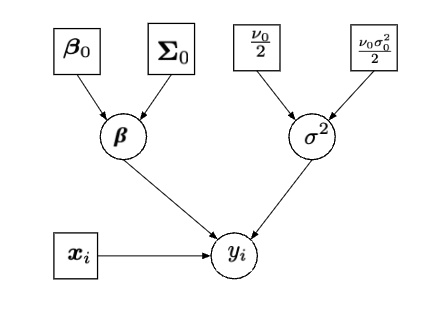
\includegraphics[scale=0.6]{Kap2/DAG_LRM.png}
    \caption{DAG Representation LRM}
    \label{fig:DAG_LRM}
\end{figure}

\subsubsection{Prior elicitation}

Prior elicitation plays a fundamental role in hierarchical linear regression, as it determines how much external information is incorporated into the posterior inference. According to \cite{SOSA}, two main strategies are commonly adopted depending on the availability of prior knowledge. When little or no external evidence is available, it is advisable to use weakly informative priors that contribute minimal influence, such as the \emph{unit information prior} of \cite{KassWasserman1995}. This choice encodes the information equivalent to a single observation and ensures that the prior does not dominate the likelihood, while still guaranteeing mathematical regularity for the posterior, \cite{HOFF} emphasizes that in regression settings, it is often convenient to center the prior mean at the ordinary least squares estimator, setting
\begin{equation}
    \bm{\beta}_0 = \hat{\bm{\beta}}_{\text{OLS}}, \qquad
    \bm{\Sigma}_0 = g \, \sigma^2 \left(\bm{X}^\top \bm{X}\right)^{-1},
\end{equation}
so that the prior on $\bm{\beta}$ represents the information of approximately one data point. Similarly, for the error variance we may use
\begin{equation}
    \nu_0 = 1, \qquad \sigma_0^2 = \hat{\sigma}^2_{\text{OLS}}.
\end{equation}
An alternative is to adopt a scale–invariant prior by setting
\begin{equation}
    \bm{\beta}_0 = \bm{0}, \qquad \bm{\Sigma}_0 = g \, \sigma^2 \left(\bm{X}^\top \bm{X}\right)^{-1},
\end{equation}
with $g=n$, leading to Zellner’s $g$‑prior \cite{Zellner1986}. Both approaches allow the researcher to encode weak or moderate prior information in a way that is consistent with model structure while remaining computationally tractable.


\subsection{Posterior Inference}

\subsubsection{Gibbs Sampling}

For this algorithm, the full conditional distributions (f.c.d.'s) of each parameter in the model $\bm{\Theta} = (\bm{\beta}, \sigma^2)$ are provided, where $p(\cdot \mid \textit{rest})$ denotes the full conditional distribution of each parameter given the remaining parameters, from the full posterior distribution as follows:

\begin{equation}
    \label{POST_LRM}
    \begin{split}
    p(\bm{\Theta} \mid \bm{y}, \bm{X}) 
    &\propto 
p(\bm{y} \mid \bm{X}, \bm{\beta}, \sigma^2) \,
p(\bm{\beta} ) \,
p(\sigma^2 )\\
&\propto\mathsf{N_n}\left(\bm{y}\mid\bm{X}\bm{\beta},\sigma^2\bm{I_n}\right)\times\mathsf{N_p}(\bm{\beta}\mid\bm{\beta}_0, \bm{\Sigma}_0)\times\mathsf{IG}\left(\sigma^2\mid\nu_0/ 2, \nu_0 \sigma_0^2 / 2\right)\\
&\propto (\sigma^2)^{-n/2} 
\exp\left\{ -\frac{1}{2\sigma^2}  (\bm{y} - \bm{X} \bm{\beta})^{\top}
(\bm{y} - \bm{X} \bm{\beta}) \right\} \\
&\quad \times \exp\left\{ -\frac{1}{2} (\bm{\beta} - \bm{\beta}_0)^{\top}
\bm{\Sigma}_0^{-1} (\bm{\beta} - \bm{\beta}_0) \right\} \\
&\quad \times (\sigma^2)^{-(\nu_0/2 + 1)} 
\exp\left\{ -\frac{\nu_0 \sigma_0^2}{2\sigma^2} \right\}
\end{split}
\end{equation}

so, the f.c.d.s are given by:

\begin{itemize}

\item f.c.d of $\bm{\beta}$

\begin{equation}
    \label{LRM_MCMC_Beta}
    \bm{\beta} \mid \text{rest} \sim \mathsf{N_p}\left(\left( \frac{1}{\sigma^2} \bm{X}^\top \bm{X} + \bm{\Sigma}_0^{-1} \right)^{-1}\left( \frac{1}{\sigma^2} \bm{X}^\top \bm{y} + \bm{\Sigma}_0^{-1} \bm{\beta}_0 \right), \left( \frac{1}{\sigma^2} \bm{X}^\top \bm{X} + \bm{\Sigma}_0^{-1} \right)^{-1}\right)
\end{equation}

\item  f.c.d of $\sigma^2$

\begin{equation}
    \label{LRM_MCMC_sigma2}
    \sigma^2 \mid \text{rest} \sim \mathsf{IG}\left( \frac{n + \nu_0}{2}, \frac{\nu_0 \sigma_0^2 + (\bm{y} - \bm{X} \bm{\beta})^\top (\bm{y} - \bm{X} \bm{\beta})}{2} \right)
\end{equation}

\end{itemize}

\begin{algorithm}[H]
\caption{Gibbs Sampling for LRM}
\begin{algorithmic}
\State \textbf{Input} Init values $\bm{\beta}^{(0)}, (\sigma^2)^{(0)}$, hyperparameters: $\bm{\beta}_0,\bm{\Sigma},\nu_0,\sigma_0^2$, data values $\bm{y},\bm{X}$
\For{$b = 1, \dots, B$}
    \State Sample $\bm{\beta}^{(b)} \sim p\left(\bm{\beta} \mid (\sigma^2)^{(b-1)},\bm{y},\bm{X}\right)$ from eq. \ref{LRM_MCMC_Beta}
    \State Sample $(\sigma^2)^{(b)} \sim p\left(\sigma^{2} \mid \bm{\beta}^{(b)},\bm{y},\bm{X}\right)$ from eq. \ref{LRM_MCMC_sigma2}
\EndFor
\State \textbf{Output} Draws $\{\bm{\beta}^{(b)}, (\sigma^2)^{(b)}\}_{b=1}^{B}$ 
\end{algorithmic}
\end{algorithm}

For detailed and explicit derivations, see Appendix \ref{Appendix_B}.


\subsubsection{CAVI}

For this algorithm, the coordinate ascent variational inference updates are presented for each parameter in the model $\bm{\Theta} = (\bm{\beta}, \sigma^2)$. Here, the updates are derived under a mean–field factorization, and each variational factor is optimized while holding the others fixed, as follows:

\begin{equation}
\label{Q_LRM}
q\left(\bm{\Theta}\right)=q(\bm{\beta})q(\sigma^2)
\end{equation}
    

\begin{itemize}

\item Factor $q(\bm{\beta}) = \mathsf{N_p}\left(\bm{\mu}_{\bm{\beta}},\bm{\Sigma}_{\bm{\beta}}\right)$, whit

\begin{equation}
\label{LRM_CAVI_Mu_Beta}
\bm{\mu}_{\bm{\beta}}=\left(\mathsf{E}_{\sigma^2}\left[ \frac{1}{\sigma^2} \right]\bm{X}^\top \bm{X} + \bm{\Sigma}_0^{-1} \right)^{-1}\left(\mathsf{E}_{\sigma^2}\left[ \frac{1}{\sigma^2}\right] \bm{X}^\top \bm{y} + \bm{\Sigma}_0^{-1} \bm{\beta}_0 \right),
\end{equation}

\begin{equation}
\label{LRM_CAVI_sigma2_Beta}
\bm{\Sigma}_{\bm{\beta}} = \left(\mathsf{E}_{\sigma^2}\left[ \frac{1}{\sigma^2} \right]\bm{X}^\top \bm{X} + \bm{\Sigma}_0^{-1} \right)^{-1}
\end{equation}

\item Factor $q(\sigma^2) = \mathsf{IG}\left( a, b \right)$, whit

\begin{equation}
\label{LRM_CAVI_a_sigma2}
a = \frac{n + \nu_0}{2},
\end{equation}

\begin{equation}
\label{LRM_CAVI_b_sigma2}
b = \frac{\nu_0 \sigma_0^2 + \mathsf{E}_{\bm{\beta}}\left[(\bm{y} - \bm{X} \bm{\beta})^{\top}
(\bm{y} - \bm{X} \bm{\beta})  \right]}{2}
\end{equation}

\item ELBO $\mathcal{L}(q(\bm{\Theta}))$

\begin{equation}
\label{LRM_CAVI_ELBO}
\begin{split}
\mathcal{L}(q(\bm{\Theta}))
&=\mathsf{E}_{\bm{\Theta}}\left[\log p(\bm{\Theta},\bm{y}, \bm{X})\right]-\mathsf{E}_{\bm{\Theta}}\left[\log q(\bm{\Theta})\right]\\
&=\mathsf{E}_{\bm{\Theta}}\left[\log p(\bm{y} \mid \bm{X}, \bm{\beta}, \sigma^2)\right] + \left(\mathsf{E}_{\bm{\Theta}}\left[\log  p(\bm{\beta})\right] -\mathsf{E}_{\bm{\beta}}\left[\log q(\bm{\beta})\right]\right)+
\left(\mathsf{E}_{\bm{\Theta}}\left[\log p(\sigma^2 )\right]-\mathsf{E}_{\sigma^2}\left[\log q(\sigma^2)\right]\right)
\end{split}
\end{equation}

\newpage

where:

\begin{itemize}
    \item $\mathsf{E}_{\bm{\Theta}}\left[\log p(\bm{y} \mid \bm{X}, \bm{\beta}, \sigma^2)\right]=-\frac{n}{2}\log(2\pi) - \frac{n}{2}\left(\log b -\psi(a)\right)
- \frac{1}{2}\left(\frac{a}{b}\right)\left((\bm{y} - \bm{X}  \bm\mu_{\bm{\beta}})^{\top}
(\bm{y} - \bm{X} \bm\mu_{\bm{\beta}}) + \operatorname{tr}\left(\bm{X}^{\top}\bm{X}\bm{\Sigma}_{\bm{\beta}}\right)\right)$
\item  $\mathsf{E}_{\bm{\Theta}}\left[\log  p(\bm{\beta})\right]=- \frac{p}{2}\log(2\pi) + \frac{1}{2}\log|\bm\Sigma_{0}|
- \frac{1}{2}
\left((\bm\mu_{\bm\beta}-\bm\beta_{0})^{\top}
\bm\Sigma_{0}^{-1}(\bm\mu_{\bm\beta}-\bm\beta_{0})+\operatorname{tr}(\bm\Sigma_0^{-1}\bm\Sigma_{\bm{\beta}})\right)$
\item $\mathsf{E}_{\bm{\beta}}\left[\log q(\bm{\beta})\right]=-\frac{d}{2}\log(2\pi e)-\frac{1}{2}\log|\bm{\Sigma}_{\bm{\beta}}|$
\item$\mathsf{E}_{\bm{\Theta}}\left[\log p(\sigma^2 )\right]=\frac{\nu_{0}}{2}\log \left(\frac{\nu_0\sigma_{0}^2}{2}\right) - \log\Gamma\left(\frac{\nu_{0}}{2}\right)
- \left(\frac{\nu_{0}}{2}+1\right)\left(\log b -\psi(a)\right)
- \frac{\nu_0\sigma_{0}^2}{2}\left(\frac{a}{b}\right)$
\item$\mathsf{E}_{\sigma^2}\left[\log q(\sigma^2)\right]=-\log b-\log\Gamma(a)+(a+1)\psi(a)-a$
\end{itemize}

\end{itemize}

\begin{algorithm}[H]
\caption{CAVI for LRM}
\begin{algorithmic}
\State \textbf{Input} Init values $\bm{\mu}_{\bm{\beta}}^{(0)}, \bm{\Sigma}_{\bm{\beta}}^{(0)}, a^{(0)}, b^{(0)}$, data values $\bm{y},\bm{X}$
\While{ELBO has not converged}
\State Update $q(\bm{\beta})$ setting $\bm{\mu}_{\bm{\beta}}$ (eq. \ref{LRM_CAVI_Mu_Beta}) and $\bm{\Sigma}_{\bm{\beta}}$ (eq. \ref{LRM_CAVI_sigma2_Beta}).
\State Update $q(\sigma^2)$ setting $a$ (eq. \ref{LRM_CAVI_a_sigma2} ) and $b$ (eq. \ref{LRM_CAVI_b_sigma2}).
\State Calculate ELBO $\mathcal{L}(q(\bm{\Theta}))$ (eq. \ref{LRM_CAVI_ELBO})
\EndWhile
\State \textbf{Output} Optimal parameters $\bm{\mu}_{\bm{\beta}}, \bm{\Sigma}_{\bm{\beta}}, a, b$
\end{algorithmic}
\end{algorithm}

For detailed and explicit derivations of these results, see Appendix \ref{Appendix_C}.



\subsection{Illustration}
\subsubsection{Iris Dataset}
To illustrate the implementation of MCMC and VI methods, we rely on a widely used benchmark dataset in statistics and machine learning: Fisher’s \textit{Iris} dataset. This dataset consists of $150$ observations of iris flowers, each described by four morphological measurements (sepal length, sepal width, petal length, and petal width), together with the species label. For the purpose of this study, we restrict attention to the relationship between petal length and sepal length. 

\begin{figure}[H]
    \centering
    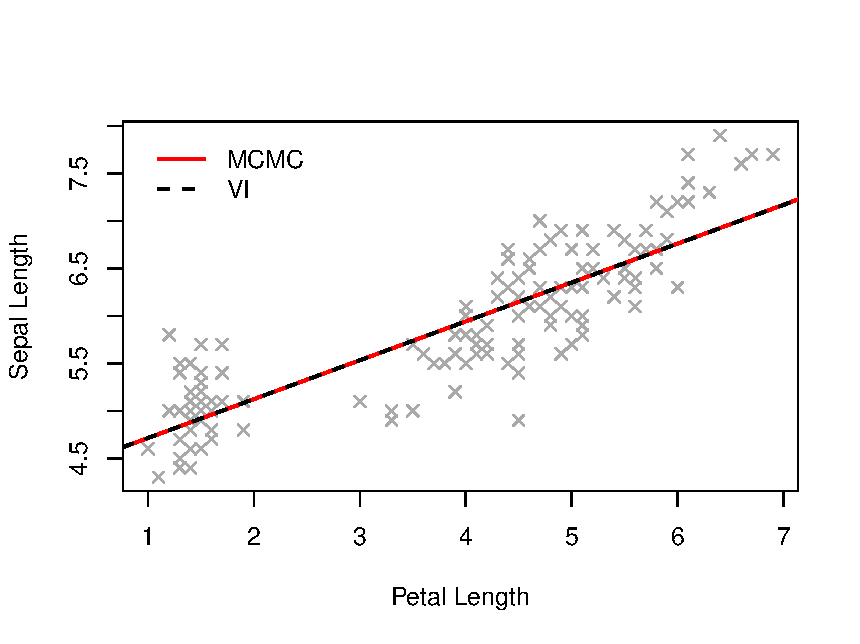
\includegraphics[scale=0.8]{Kap3/lrm_scatter.pdf}
    \caption{Scatterplot of sepal length (y-axis) against petal length (x-axis) for the \textit{Iris} dataset with estimated regression lines obtained via MCMC and VI.}
    \label{fig:lrm_scatter}
\end{figure}


Figure \ref{fig:lrm_scatter} shows similar results under both methodologies, and Table \ref{tab:fit_lr} provides a quantitative comparison of their performance. In particular, both MCMC and VI yield almost identical values for the information criteria (WAIC and DIC), as well as for the predictive accuracy metrics ($R^2$ and MSE). This confirms that the variational approximation provides an accurate posterior representation in this simple regression setting. However, a substantial difference arises in terms of computational efficiency: while MCMC requires approximately 21 seconds to complete, the VI method converges in about 1 second. This highlights one of the main advantages of variational inference, namely its ability to deliver results of comparable quality to MCMC but at a fraction of the computational cost.
 
\begin{table}[ht]
\centering
\caption{Goodness of fit and runtime (LRM, 1000 posterior samples), Iris Dataset.}
\label{tab:fit_lr}
\begin{tabular}{lrr}
\toprule
Metric & MCMC & VI \\
\midrule
WAIC & 160.061 & 160.259 \\
DIC & 160.028 & 160.215 \\
$R^2$ & 0.760 & 0.760 \\
MSE & 0.164 & 0.164 \\
Time (sec) & 21.184 & 1.008 \\
\bottomrule
\end{tabular}
\end{table}

\newpage

Figure \ref{fig:lrm_ELBO} illustrates the evolution of the Evidence Lower Bound (ELBO) as a function of execution time. The solid red curve corresponds to the VI optimization path, while the dashed blue line represents the posterior mean log-joint estimated via MCMC. As observed, the VI method rapidly increases the ELBO during the first iterations, reaching a stable plateau that closely approximates the MCMC benchmark within a fraction of a second. This behavior highlights the fast convergence properties of variational inference, which achieves a comparable approximation to the posterior distribution obtained by MCMC but with a substantially lower computational cost. In contrast, MCMC delivers a more robust estimate of the log-joint expectation, though at the expense of significantly longer execution time.


\begin{figure}[H]
    \centering
    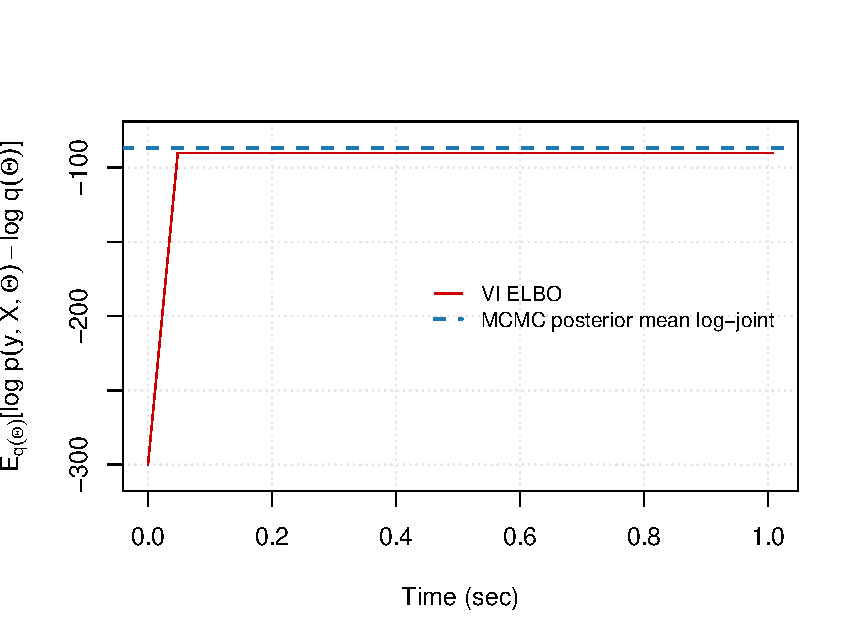
\includegraphics[scale=0.7]{Kap3/lrm_elbo_logjoint.pdf}
    \caption{Evolution of the ELBO compared with the posterior mean log-joint probability estimated via MCMC for LRM.}
    \label{fig:lrm_ELBO}
\end{figure}

Figure \ref{fig:lrm_betas_joint} presents the estimated joint posterior density for the regression coefficients 
$\bm{\beta} = (\beta_1, \beta_2)$ in the Iris dataset. The gray points correspond to MCMC draws, while the solid 
and dashed contours represent the $50\%$ and $95\%$ Mahalanobis credible regions obtained under MCMC and VI, 
respectively. Both methods yield highly consistent estimates of the joint distribution, with posterior means 
indicated by the vertical and horizontal lines. 

\vspace{0.5cm}

The overlap between the MCMC and VI contours indicates that the variational approximation is able to capture 
the main correlation structure between $\beta_1$ and $\beta_2$, as well as the shape and orientation of the 
joint posterior distribution. Moreover, the marginal credible intervals obtained from VI closely align with 
those derived from MCMC, demonstrating that in this setting the variational method achieves nearly the same 
precision as the MCMC approach, while offering substantial gains in computational efficiency.

\begin{figure}[H]
    \centering
    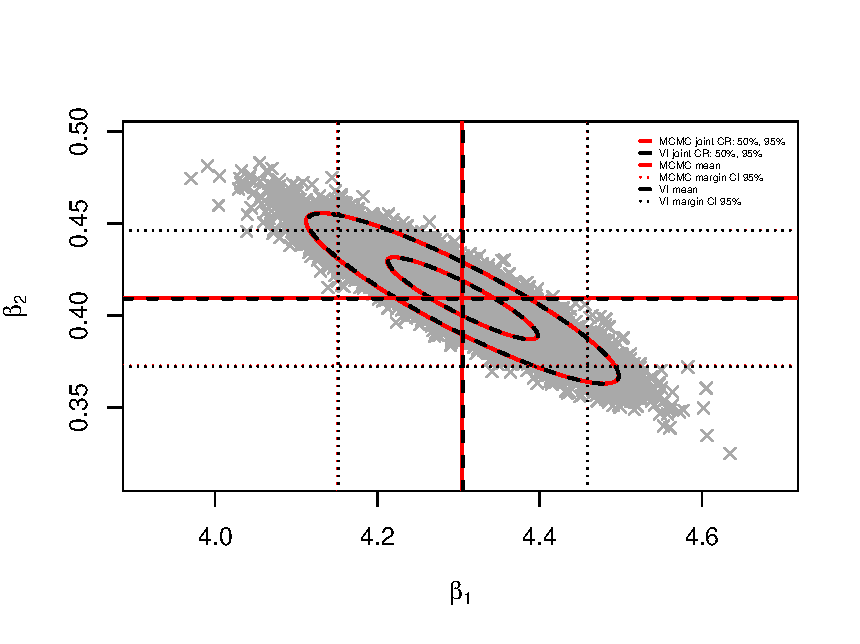
\includegraphics[scale=0.8]{Kap3/lrm_betas_joint.pdf}
    \caption{Joint posterior density estimates for $\bm{\beta} = (\beta_1, \beta_2)$ in the LRM using the Iris dataset, including Mahalanobis credible regions obtained via MCMC and VI and margin credible intervals.}
    \label{fig:lrm_betas_joint}
\end{figure}


\begin{figure}[H]
    \centering
    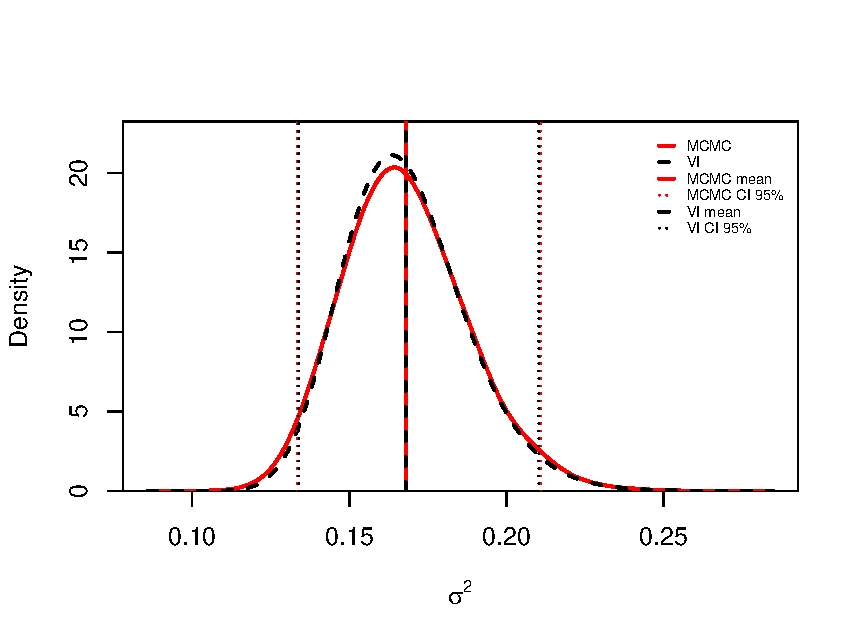
\includegraphics[scale=0.7]{Kap3/lrm_sigma2_density.pdf}
    \caption{Posterior density estimates for the error variance $\sigma^2$ in the LRM using the Iris dataset.}
    \label{fig:lrm_sigma2}
\end{figure}

\newpage

Figure \ref{fig:lrm_sigma2} shows the estimated posterior density of the error variance $\sigma^2$ under both 
MCMC and VI approaches. The two curves are nearly indistinguishable, with posterior means centered around 
$0.168$ and highly similar credible intervals. The vertical lines denote the posterior means, while the dotted 
lines correspond to the $95\%$ credible intervals under each method. Both approaches capture the uncertainty 
around $\sigma^2$ in a consistent manner, with VI closely approximating the posterior spread obtained from MCMC. 

\begin{table}[ht]
\centering
\caption{Posterior summaries LRM under MCMC and VI, Iris Dataset}
\label{tab:post_mcmc_vi}
\begin{tabular}{lcccccc}
\toprule
& \multicolumn{2}{c}{Mean} & \multicolumn{2}{c}{SD} & \multicolumn{2}{c}{CI} \\
\cmidrule(lr){2-3}\cmidrule(lr){4-5}\cmidrule(lr){6-7}
Parameter & MCMC & VI & MCMC & VI & MCMC & VI \\
\midrule
$\bm\beta_{1}$ & 4.305 & 4.306 & 0.079 & 0.078 & $[4.151, 4.458]$ & $[4.152, 4.459]$ \\
$\bm\beta_{2}$& 0.409 & 0.409 & 0.019 & 0.019 & $[0.373, 0.446]$ & $[0.372, 0.446]$ \\
$\sigma^2_{1}$ & 0.168 & 0.168 & 0.020 & 0.020 & $[0.133, 0.211]$ & $[0.134, 0.210]$ \\
\bottomrule
\end{tabular}
\end{table}

Table \ref{tab:post_mcmc_vi} further summarizes the posterior results. For $\sigma^2$, both methods report 
identical posterior means ($0.168$), standard deviations ($0.020$), and very similar $95\%$ credible intervals 
($[0.133,0.211]$ for MCMC versus $[0.134,0.210]$ for VI). These results confirm that, in this case, 
variational inference provides not only accurate point estimates but also a reliable approximation 
of posterior uncertainty relative to MCMC.

\subsubsection{Simulation}

With the purpose of assessing the performance of the proposed inference methodologies under controlled conditions, a simulation study was conducted in which each scenario is defined by the sample size $n$ and the number of predictors $p$, with true parameter values specified in the simulation design. For the case $p=3$, the regression coefficients were set to $\bm{\beta}=(25,10,-30)^\top$ with error variance $\sigma^2=100^2$, while for $p=2$ the coefficients were $\bm{\beta}=(2,-12)^\top$ with $\sigma^2=4^2$. Sample sizes $n=50,100,1000$ were considered for each configuration.

\vspace{0.5cm}

These configurations were chosen to evaluate the behavior of the inference methods across varying levels of model complexity and information content. In particular, increasing $n$ allows us to examine how the variational approximation improves as more data become available, while varying $p$ controls the dimensionality of the parameter space. Performance is assessed in terms of posterior mean accuracy, uncertainty quantification, and overall posterior approximation quality, using MCMC as a reference benchmark. Table~\ref{tab:method_quality} summarizes the performance of MCMC and VI across six simulation scenarios.

\begin{table}[ht]
\centering
\caption{Posterior zero coverage LRM under MCMC and VI in the $95\%$ CI, and runtime across simulation scenarios. }
\label{tab:method_quality}
\begin{tabular}{ccccccccc}
\toprule
 & & & \multicolumn{3}{c}{\textbf{MCMC}} & \multicolumn{3}{c}{\textbf{VI}} \\
\cmidrule(lr){4-6}\cmidrule(lr){7-9}
  n & p & \#params & $0 \in CI$ & Truth $\in $ CI & Time (s) & $0\in CI$ & Truth $\in$ CI & Time (s) \\

  50   & 3 & 4 & 3/4 (75.0\%)  & 4/4 (100.0\%) & 13.73 & 3/4 (75.0\%)  & 4/4 (100.0\%) & 0.59 \\
  100  & 3 & 4 & 3/4 (75.0\%)  & 4/4 (100.0\%) & 13.57 & 3/4 (75.0\%)  & 4/4 (100.0\%) & 0.59 \\
  1000 & 3 & 4 & 3/4 (75.0\%)  & 4/4 (100.0\%) & 14.67 & 3/4 (75.0\%)  & 4/4 (100.0\%) & 0.69 \\
  50   & 2 & 3 & 1/3 (33.3\%)  & 3/3 (100\%)  & 11.69 & 1/3 (33.3\%)  & 2/3 (66.7\%)  & 0.00 \\
  100  & 2 & 3 & 0/3 (0.0\%)   & 3/3 (100.0\%) & 11.80 & 0/3 (0.0\%)   & 3/3 (100.0\%) & 0.00 \\
  1000 & 2 & 3 & 0/3 (0.0\%)   & 3/3 (100.0\%) & 12.70 & 0/3 (0.0\%)   & 3/3 (100.0\%) & 0.00 \\
\bottomrule
\end{tabular}
\end{table}

\newpage

The metrics reported include (i) the proportion of parameters for which zero lies inside the $95\%$ posterior 
credible interval ($0 \in CI$), (ii) the proportion of true parameter values contained in the posterior 
credible interval (coverage), and (iii) the runtime in seconds. As expected, both methods exhibit perfect 
coverage of the true parameters across all scenarios ($100\%$ in almost all cases), while the presence of zero 
within the credible interval varies according to the underlying coefficients. This reflects the fact that the 
posterior distributions correctly exclude or include zero depending on whether the true effect is large or small. 

\vspace{0.5cm}

A striking difference appears in computational cost: MCMC requires between $11$ and $15$ seconds of execution 
time regardless of the sample size, while VI completes in less than one second for $p=3$ and virtually zero 
time for $p=2$. These results confirm that VI attains accuracy comparable to MCMC in terms of posterior 
coverage while offering substantial gains in computational efficiency, particularly in larger-scale settings.

\section{Hierarchical Normal Linear Regression Model}

The hierarchical linear models are extensions of linear regression models , where we can include a grouping structure present in data, as stated by
\cite{GELMAN}  , for examples persons within cities, students in schools, even repeated measures on the same individual. All of these cases present an hierarchical structure where the levels of these are taken as hierarchies, which implies that we can propose a linear regression where the regression coefficients can varying trough by group (Intercept and slopes). The inclusion of these structures can show a more accurately description and posterior inferences for the individuals, taking in account the specific information within the group and showing difference between groups.

\newpage

In \cite{HOFF} it describes the hierarchical linear model as a generalization of normal hierarchical model where we can compare multiple groups taking account the heterogeneity across several populations and  heterogeneity within the groups even including an specific behavior per group, to extend the results, the ordinary regression model is used to describe within-group heterogeneity of observations, then describe between-group heterogeneity using a sampling model for the group-specific regression parameters,as follows:

\begin{equation}
\label{HRLM}
y_{ij} \mid \bm{x}_{ij}, \bm{\beta}_j, \sigma_j^2 \stackrel{\text { ind }}{\sim} \mathsf{N}\left(\bm{x}_{ij}^{\bm{\top}} \bm{\beta}_j, \sigma_j^2\right), \quad i=1, \ldots, n_j, \quad j=1, \ldots, m
\end{equation}

Where $\bm{x}_{ij}$ is a $p \times 1$ vector of regressors for observation $i$ in group $j$,  $\bm{y}_j = \left[y_{1j}, \ldots, y_{n_j, j}\right]^\top$  is a $n_j \times 1$ vector of response variable values for group $j$  and $\mathbf{X}_j = \left[\bm{x}_{1j}, \ldots, \bm{x}_{n_j, j}\right]^\top$ a $n_j \times p$ matrix , the within-group sampling model can be expressed equivalently as $\bm{y}_j \sim$  $\mathsf{N_p}\left(\mathbf{X}_j \bm{\beta}_j, \sigma^2_j \mathbf{I}_p\right)$, with the group-specific data vectors $\bm{y}_1, \ldots, \bm{y}_m$ being conditionally independent given all $\bm{\beta}_j$ and $\sigma^2_j$.

\subsection{Prior Distributions}

In order to specify a Bayesian point of view to estimate the parameters   \cite{SOSA} propose define the priors distributions for the parameters vector $\bm{\Theta}=(\bm{\xi},\bm{\sigma^2},\bm{\beta},\bm{\Sigma},\xi^2)$ with $\bm{\xi}=(\bm{\beta}_1, \ldots, \bm{\beta}_m)$,    $\bm{\beta}_j=(\beta_{1j},\cdots,\beta_{pj})$ and $\bm{\sigma^2}=(\sigma_1^2,\cdots,\sigma_m^2)$  for model described in figure \ref{HRLM} represented by \ref{fig:DAG_HLRM}, as follows:

\begin{equation}
    \label{hyper_HRLM_1}
    \bm{\beta}_j \mid \bm{\beta}, \bm{\Sigma} \stackrel{\mathsf{iid}}{\sim} \mathsf{N}_p(\bm{\beta}, \bm{\Sigma}) \quad \text { and } \quad \sigma_j^2 \mid \xi^2 \stackrel{\mathsf{iid}}{\sim} \mathsf{IG}\left(\nu_0 / 2, \nu_0 \xi^2 / 2\right)
\end{equation}

\begin{equation}
    \label{hyper_HRLM_2}
    \bm{\beta} \sim \mathsf{N_p}\left(\bm{\mu}_0, \bm{\Lambda}_0\right), \quad \bm{\Sigma} \sim \mathsf{IW}\left(n_0, \mathbf{S}_0^{-1}\right), \quad \xi^2 \sim \mathsf{G}\left(a_0, b_0\right)
\end{equation}

with $\bm{\mu}_0, \bm{\Lambda}_0, n_0, \mathbf{S}_0, \nu_0, a_0, \text { and } b_0$ the hyperparameters of model.

\begin{figure}[H]
    \centering
    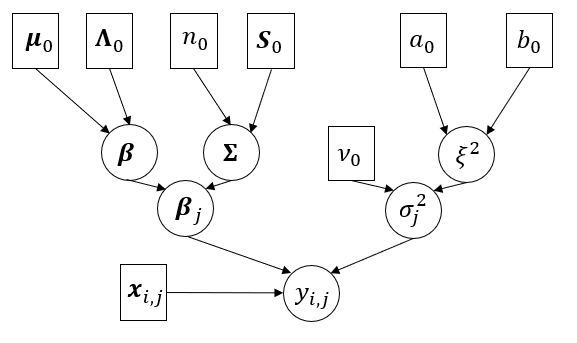
\includegraphics[scale=0.8]{Kap2/DAG_HLRM.png}
    \caption{DAG Representation HLRM}
    \label{fig:DAG_HLRM}
\end{figure}

\subsubsection{Prior Elicitation}

\cite{KassWasserman1995} and \cite{SOSA} adopt the unit–information–prior perspective, under which the hyperparameters for the HLRM are specified to yield a weak but coherent prior configuration. In particular, we define $g = \sum_{j=1}^{m} n_j$ and fix $\nu_0 = 1$, while the location parameter is taken as $\bm{\mu}_0 = \hat{\bm{\beta}}_{\text{OLS}}$. The scale matrix is set to $\bm{\Lambda}_0 = g\,\hat{\sigma}^2_{\text{OLS}}(\bm{X}^\top\bm{X})^{-1}$, with $\hat{\sigma}^2_{\text{OLS}}$ denoting the residual variance from the OLS fit. For the covariance hyperparameters, we choose $n_0 = p + 2$ and $\bm{S}_0 = \bm{\Lambda}_0$, a combination that produces a diffuse yet centered concentration around $\bm{\mu}_0$. Lastly, for the variance component, the settings $a_0 = 1$ and $b_0 = 1/\hat{\sigma}^2_{\text{OLS}}$ are adopted, ensuring that $\mathsf{E}(\xi^2) = \hat{\sigma}^2_{\text{OLS}}$, which produces a diffuse prior.

\subsection{Posterior Inference}

\subsubsection{Gibbs Sampling}

Once again we derivate the f.c.d's for each parameter in $\bm{\Theta}=(\bm{\zeta},\bm{\sigma^2},\bm{\beta},\bm{\Sigma},\xi^2)$ starting from the full posterior distribution, this is:

\begin{equation}
\begin{split}
    \label{POST_HLRM}
    p(\bm{\Theta} \mid\bm{y}, \bm{X}) 
    &\propto p(\bm{y} \mid \bm{X}, \bm{\zeta} ,\bm{\sigma^2}) 
p(\bm{\zeta} \mid \bm{\beta}, \bm{\Sigma}) 
p(\bm{\beta}) 
p(\bm{\Sigma}) 
p(\bm{\sigma^2}\mid 
\xi^2)
p(\xi)\\
&\propto \prod_{j=1}^{m}\mathsf{N}_{n_j}(\bm{y}_{j}\mid\bm{X}_{j} \bm{\beta}_j,{\sigma}_j^2)\times\prod_{j=1}^{m}\mathsf{N_p}(\bm{\beta}_j \mid \bm{\beta}, \bm{\Sigma})\times\mathsf{N_p}(\bm{\beta}\mid\bm{\mu}_0, \bm{\Lambda}_0)\\
&\quad\times\mathsf{IW}\left(\bm{\Sigma}\mid n_0, \mathbf{S}_0^{-1}\right)\times\prod_{j=1}^{m}\mathsf{IG}\left(\sigma_j^2 \mid\nu_0 / 2, \nu_0 \xi^2 / 2\right)\times\mathsf{G}\left(\xi^2 \mid a_0, b_0\right)\\
&\propto \prod_{j=1}^{m}  ({\sigma}_j^2)^{-n_j/2} 
\exp\left\{ -\frac{1}{2\sigma_j^2} (\bm{y}_{j} - \bm{X}_{j} \bm{\beta}_j)^\top(\bm{y}_{j} - \bm{X}_{j} \bm{\beta}_j) \right\} \\
&\quad\times \prod_{j=1}^{m} \left| \bm{\Sigma} \right|^{-1/2} 
\exp\left\{ -\frac{1}{2} (\bm{\beta}_j -  \bm{\beta})^\top \bm{\Sigma}^{-1} (\bm{\beta}_j - \bm{\beta}) \right\} \\
&\quad \times \exp\left\{ -\frac{1}{2} (\bm{\beta} - \bm{\mu}_0)^\top \bm{\Lambda}_0^{-1} (\bm{\beta} - \bm{\mu}_0) \right\}
\times |\bm{\Sigma}|^{-(n_0 + p + 1)/2} 
 \exp\left\{ -\frac{1}{2} \mathrm{tr}(\bm{S}_0 \bm{\Sigma}^{-1}) \right\} \\
&\quad \times \prod_{j=1}^{m} (\xi^2)^{\nu_0 / 2 - 1} 
(\sigma_j^2)^{-(\nu_0 / 2+1)} 
\exp\left\{ -\frac{\nu_0 \xi^2}{2 \sigma_j^2} \right\} 
\times (\xi^2)^{a_0 - 1} \exp\left\{ -b_0 \xi^2 \right\}
\end{split}
\end{equation}

then, the f.c.d.s for this model are:

\begin{itemize}
    \item f.c.d of $\bm{\beta}_j$ for $j=1,\dots,m$
    \begin{equation}
        \label{HLRM_MCMC_Betaj}
        \bm{\beta}_j \mid \text{rest} \sim \mathsf{N_p} \left( 
\left[ ({\sigma_j}^{-2}) \bm{X}_{j} \bm{X}_{j}^\top + \bm{\Sigma}^{-1} \right]^{-1}
\left[ ({\sigma_j}^{-2}) \bm{X}_{j}^\top \bm{y}_{j} + \bm{\Sigma}^{-1} \bm{\beta} \right], \ 
\left[ (\sigma_j^{-2}) \bm{X}_{j} \bm{X}_{j}^\top  + \bm{\Sigma}^{-1} \right]^{-1}
\right)
    \end{equation}
    \item f.c.d of $\bm{\beta}$
    \begin{equation}
        \label{HLRM_MCMC_Beta}
        \bm{\beta} \mid \text{rest} \sim \mathsf{N}_p \left(
\left( \bm{\Lambda}_0^{-1} + m \bm{\Sigma}^{-1} \right)^{-1}
\left( \bm{\Lambda}_0^{-1} \bm{\mu}_0 + \bm{\Sigma}^{-1} \sum_{j=1}^{m} \bm{\beta}_j \right),
\left( \bm{\Lambda}_0^{-1} + m \bm{\Sigma}^{-1} \right)^{-1}\right)
    \end{equation}
    \item f.c.d of $\bm{\Sigma}$
    \begin{equation}
        \label{HLRM_MCMC_Sigma}
        \bm{\Sigma} \mid \text{rest} \sim \mathsf{IW} \left( 
n_0 + m,\ 
\left( \bm{S}_0 + \sum_{j=1}^{m} (\bm{\beta}_j - \bm{\beta})(\bm{\beta}_j - \bm{\beta})^\top\right)^{-1}
\right)
    \end{equation}
    
\item f.c.d of $\sigma_j^2$ for $j=1,\dots,m$
    
    \begin{equation}
        \label{HLRM_MCMC_sigma2j}
        \sigma_j^2 \mid \text{rest} \sim \mathsf{IG} \left( 
\frac{n_j + \nu_0}{2},\ 
\frac{ \nu_0 \xi^2 +  (\bm{y}_{j} - \bm{X}_{j} \bm{\beta}_j)^\top(\bm{y}_{j} - \bm{X}_{j} \bm{\beta}_j)}{2} 
\right)
    \end{equation}
    \item f.c.d of $\xi^2$
    \begin{equation}
        \label{HLRM_MCMC_xi2}
        \xi^2 \mid \text{rest} \sim \mathsf{G} \left(
\frac{m \nu_0}{2} + a_0,\ 
b_0 + \frac{\nu_0}{2} \sum_{j=1}^{m} \sigma_j^{-2}
\right)
    \end{equation}
\end{itemize}

\begin{algorithm}[H]
\caption{Gibbs Sampling for HLRM}
\begin{algorithmic}
\State \textbf{Input} Init values $\{\bm{\beta}_j^{(0)}\}_{j=1}^m,\; \bm{\beta}^{(0)},\; \bm{\Sigma}^{(0)},\; \{\sigma_j^{2(0)}\}_{j=1}^m,\; \xi^{2(0)}$, hyperparameters $\bm{\mu}_0,\bm{\Lambda}_0, n_0,\bm{S}_0,a_0,b_0,\nu_0,\sigma_0^2$, data values $\{\bm{y}_j,\bm{X}_j\}_{j=1}^m$

\For{$b = 1, \dots, B$}
  \For{$j = 1, \dots, m$}
    \State Sample $\bm{\beta}_j^{(b)} \sim p\!\left(\bm{\beta}_j \mid \bm{\beta}^{(b-1)},\bm{\Sigma}^{(b-1)},(\sigma_j^2)^{(b-1)},\bm{y}_j,\bm{X}_j\right)$ from eq. \ref{HLRM_MCMC_Betaj}
    \State Sample $(\sigma_j^2)^{(b)} \sim p\!\left(\sigma_j^2 \mid \bm{\beta}_j^{(b)},(\xi^2)^{(b-1)},\bm{y}_j,\bm{X}_j\right)$ from eq. \ref{HLRM_MCMC_sigma2j}
  \EndFor
  \State Sample $\bm{\beta}^{(b)} \sim p\!\left(\bm{\beta} \mid \{\bm{\beta}_j^{(b)}\},\bm{\Sigma}^{(b-1)}\right)$ from eq. \ref{HLRM_MCMC_Beta}
  \State Sample $\bm{\Sigma}^{(b)} \sim p\!\left(\bm{\Sigma} \mid \{\bm{\beta}_j^{(b)}\},\bm{\beta}^{(b)}\right)$ from eq. \ref{HLRM_MCMC_Sigma}
  \State Sample $(\xi^2)^{(b)} \sim p\!\left(\xi^2 \mid \{(\sigma_j^2)^{(b)}\}\right)$ from eq. \ref{HLRM_MCMC_xi2}
\EndFor
\State \textbf{Output} Draws $\{\bm{\beta}_j^{(b)},(\sigma_j^2)^{(b)},\bm{\beta}^{(b)},\bm{\Sigma}^{(b)},(\xi^2)^{(b)}\}_{b=1}^B$
\end{algorithmic}
\end{algorithm}

For detailed and explicit derivations of these results, see Appendix \ref{Appendix_B}.

\subsubsection{CAVI}

As before, we define the variational distribution to approximate the posterior distribution under the mean–field assumption described in result \ref{MFA}. Using the CAVI results for exponential family models in \ref{NMVFB_opt}, we derive the variational parameters for each factor. It is important to note that these variational parameters can be decomposed into local parameters, which are specific to each group $j$, and global parameters, which correspond to latent variables shared across all groups.


\begin{equation}
\label{Q_HLRM}
\begin{split}
q(\bm{\Theta})&=\prod_{j=1}^{m}q(\bm{\beta}_j)q(\bm{\beta})q(\bm{\Sigma})\prod_{j=1}^{m}q(\sigma_j^2)q(\xi^2)\\
&= \left(\prod_{j=1}^{m}q(\bm{\beta}_j)q(\sigma_j^2)\right)\left(q(\bm{\beta})q(\bm{\Sigma})q(\xi^2)\right)
\end{split}
\end{equation}

\begin{itemize}
    \item Factor $q(\bm{\beta}_j)=\mathsf{N_p}(\bm{\mu}_{\bm{\beta}_j},\bm{\Sigma}_{\bm{\beta}_j})$  for $j=1,\dots,m$, with

\begin{equation}
\label{HLRM_CAVI_Sigma_Betaj}
\bm{\Sigma}_{\bm{\beta}_j} = \left[ \mathsf{E}_{\sigma^2_j}\left[{\sigma_j}^{-2}\right] \bm{X}_{j} \bm{X}_{j}^\top  + \mathsf{E}_{\bm{\Sigma}}\left[\bm{\Sigma}^{-1}\right]  \right]^{-1},
\end{equation}

\begin{equation}
\label{HLRM_CAVI_Mu_Betaj}
\bm{\mu}_{\bm{\beta}_j}= \left[ \mathsf{E}_{\sigma^2_j}\left[{\sigma_j}^{-2}\right] \bm{X}_{j} \bm{X}_{j}^\top  + \mathsf{E}_{\bm{\Sigma}}\left[\bm{\Sigma}^{-1}\right]  \right]^{-1}\left[\mathsf{E}_{\sigma^2_j}\left[{\sigma_j}^{-2}\right] \bm{X}_{j}^\top \bm{y}_{j} + \mathsf{E}_{\bm{\Sigma}}\left[\bm{\Sigma}^{-1}\right] \mathsf{E}_{\bm{\beta}}\left[\bm{\beta} \right] \right]
\end{equation}

\item Factor $q(\bm{\beta})=\mathsf{N_p}(\bm{\mu}_{\bm{\beta}},\bm{\Sigma}_{\bm{\beta}})$, with

\begin{equation}
\label{HLRM_CAVI_Sigma_Beta}
\bm{\Sigma}_{\bm{\beta}} = \left[\bm{\Lambda}_0^{-1}   + \sum_{j=1}^{m}\mathsf{E}_{\bm{\Sigma}}\left[\bm{\Sigma}^{-1}\right]  \right] ^{-1},
\end{equation}

\begin{equation}
\label{HLRM_CAVI_Mu_Beta}
\bm{\mu}_{\bm{\beta}}= \left[\bm{\Lambda}_0^{-1}   + \sum_{j=1}^{m}\mathsf{E}_{\bm{\Sigma}}\left[\bm{\Sigma}^{-1}\right]  \right]^{-1}\left[\bm{\Lambda}_0^{-1} \bm{\mu}_0 + \sum_{j=1}^{m}\mathsf{E}_{\bm{\Sigma}}\left[\bm{\Sigma}^{-1}\right] \mathsf{E}_{\bm{\beta}_j}\left[\bm{\beta}_j \right]\right]
\end{equation}

    \item Factor $q(\bm{\Sigma})=\mathsf{IW}(\nu_{\bm{\Sigma}},\bm{S}_{\bm{\Sigma}}^{-1})$, with

\begin{equation}
\label{HLRM_CAVI_nu_Sigma}
\nu_{\bm{\Sigma}} = n_0+m,
\end{equation}

\begin{equation}
\label{HLRM_CAVI_S_Sigma}
\bm{S}_{\bm{\Sigma}}=  \bm{S}_0 + \sum_{j=1}^{m} \mathsf{E}_{\bm{\beta}_j,\bm{\beta}}\left[\left(\bm{\beta}_j - \bm{\beta})(\bm{\beta}_j - \bm{\beta}\right)^\top\right]
\end{equation}
    
    \item Factor $q(\sigma_j^2)=\mathsf{IG}(a_{\sigma_j^2},b_{\sigma_j^2})$ for $j=1,\dots,m$, with

\begin{equation}
\label{HLRM_CAVI_a_sigma2j}
a_{\sigma_j^2}= \frac{n_j + \nu_0}{2},
\end{equation}

\begin{equation}
\label{HLRM_CAVI_b_sigma2j}
b_{\sigma_j^2}= \frac{ \nu_0 \mathsf{E}_{\xi^2}\left[\xi^2\right] +  \mathsf{E}_{\bm{\beta}_j}\left[\left(\bm{y}_{j} - \bm{X}_{j} \bm{\beta}_j)^\top(\bm{y}_{j} - \bm{X}_{j} \bm{\beta}_j\right)\right]}{2}
\end{equation}

    \item Factor $q(\xi^2)=\mathsf{G}(a_{\xi^2},b_{\xi^2})$, with

\begin{equation}
\label{HLRM_CAVI_a_xi2}
a_{\xi^2}=  a_0 +\frac{m \nu_0}{2},
\end{equation}

\begin{equation}
\label{HLRM_CAVI_b_xi2}
b_{\xi^2}= b_0 + \frac{\nu_0}{2} \sum_{j=1}^{m} \mathsf{E}_{\sigma^2_j}\left[\sigma_j^{-2}\right]
\end{equation}

\item ELBO $\mathcal{L}(q(\bm{\Theta}))$

\begin{equation}
\label{HLRM_CAVI_ELBO}
\begin{split}
\mathcal{L}(q(\bm{\Theta}))
&=\mathsf{E}_{\bm{\Theta}}\left[\log p(\bm{\Theta},\bm{y}, \bm{X})\right]-\mathsf{E}_{\bm{\Theta}}\left[\log q(\bm{\Theta})\right]\\
&= \sum_{j=1}^{m} \mathsf{E}_{\bm{\Theta}}\left[\log p\left(\bm{y}_j \mid \bm{\beta}_j, \sigma_j^2, \mathbf{X}_j \right)\right]+\sum_{j=1}^{m} \left(\mathsf{E}_{\bm{\Theta}}\left[\log p\left(\bm{\beta}_j \mid \bm{\beta}, \bm{\Sigma}\right)\right]-\mathsf{E}_{\bm{\beta}_j}\left[\log q(\bm{\beta}_j)\right]\right) \\ 
&\quad + \left(\mathsf{E}_{\bm{\Theta}}\left[\log p(\bm{\beta})\right]-\mathsf{E}_{\bm{\beta}}\left[\log q\left(\bm{\beta}\right)\right]\right)+\left(\mathsf{E}_{\bm{\Theta}}\left[\log p\left(\bm{\Sigma}\right)\right]- \mathsf{E}_{\bm{\Sigma}}\left[\log q(\bm{\Sigma})\right]\right) \\
&\quad + \sum_{j=1}^{m} \left(\mathsf{E}_{\bm{\Theta}}\left[\log p\left(\sigma^2_j\mid\xi^2\right)\right]-\mathsf{E}_{\sigma^2_j}\left[\log q\left(\sigma^2_j\right) \right]\right) + \left(\mathsf{E}_{\bm{\Theta}}\left[\log p(\xi^2)\right] - \mathsf{E}_{\xi^2}\left[\log q(\xi^2)\right]\right)
\end{split}
\end{equation}

where:

\begin{itemize}

\item
$
\begin{aligned}
\mathsf{E}_{\bm{\Theta}}\left[\log p\left(\bm{y}_j \mid \bm{\beta}_j, \sigma_j^2, \mathbf{X}_j \right)\right]
&= -\tfrac{n_j}{2}\log(2\pi)
-\tfrac{n_j}{2}\left(\log b_{\sigma_j^2}-\psi(a_{\sigma_j^2})\right) \\
&\quad -\tfrac{1}{2}\left(\tfrac{a_{\sigma_j^2}}{b_{\sigma_j^2}}\right)
\Big[
(\bm{y}_j-\mathbf{X}_j\bm{\mu}_{\bm{\beta}_j})^\top(\bm{y}_j-\mathbf{X}_j\bm{\mu}_{\bm{\beta}_j})
+\operatorname{tr}\!\left(\mathbf{X}_j^\top\mathbf{X}_j\,\bm{\Sigma}_{\bm{\beta}_j}\right)
\Big]
\end{aligned}
$

\item
$
\begin{aligned}
\mathsf{E}_{\bm{\Theta}}\left[\log p\left(\bm{\beta}_j \mid \bm{\beta}, \bm{\Sigma}\right)\right]
&= -\tfrac{p}{2}\log(2\pi)
-\tfrac{1}{2}\Bigg(
-\sum_{i=1}^{p}\psi\left(\tfrac{\nu_{\bm{\Sigma}}+1-i}{2}\right)
-p\log 2 + \log|\bm{S}_{\bm{\Sigma}}^{-1}|
\Bigg) \\
&\qquad -\tfrac{1}{2}\operatorname{tr}\left(\bm{S}_{\bm{\Sigma}}^{-1}\left[
(\bm{\mu}_{\bm{\beta}_j}-\bm{\mu}_{\bm{\beta}})
(\bm{\mu}_{\bm{\beta}_j}-\bm{\mu}_{\bm{\beta}})^\top
+\bm{\Sigma}_{\bm{\beta}_j}+\bm{\Sigma}_{\bm{\beta}}
\right]\right)
\end{aligned}
$

\item
$
\mathsf{E}_{\bm{\beta}_j}\left[\log q(\bm{\beta}_j)\right]
= -\tfrac{p}{2}\log(2\pi e)-\tfrac{1}{2}\log|\bm{\Sigma}_{\bm{\beta}_j}|
$

\item
$
\begin{aligned}
\mathsf{E}_{\bm{\Theta}}\left[\log p(\bm{\beta})\right]
&= -\tfrac{p}{2}\log(2\pi)-\tfrac{1}{2}\log|\bm{\Lambda}_0| -\tfrac{1}{2}\left[
(\bm{\mu}_{\bm{\beta}}-\bm{\mu}_0)^\top\bm{\Lambda}_0^{-1}(\bm{\mu}_{\bm{\beta}}-\bm{\mu}_0)
+\operatorname{tr}\!\left(\bm{\Lambda}_0^{-1}\bm{\Sigma}_{\bm{\beta}}\right)
\right]
\end{aligned}
$

\item
$
\mathsf{E}_{\bm{\beta}}\left[\log q\left(\bm{\beta}\right)\right]
= -\tfrac{p}{2}\log(2\pi e)-\tfrac{1}{2}\log|\bm{\Sigma}_{\bm{\beta}}|
$

\item
$
\begin{aligned}
\mathsf{E}_{\bm{\Theta}}\left[\log p\left(\bm{\Sigma}\right)\right]
&= \tfrac{n_0}{2}\log|\bm{S}_0|-\tfrac{n_0 p}{2}\log 2-\log\Gamma_p\left(\tfrac{n_0}{2}\right)  -\tfrac{n_0+p+1}{2}\Bigg(
-\sum_{i=1}^{p}\psi\!\left(\tfrac{\nu_{\bm{\Sigma}}+1-i}{2}\right)-p\log 2+\log|\bm{S}_{\bm{\Sigma}}^{-1}|
\Bigg) \\
&\quad -\tfrac{1}{2}\operatorname{tr}\left(\bm{S}_0\,\bm{S}_{\bm{\Sigma}}^{-1}\right)
\end{aligned}
$

\item
$
\begin{aligned}
\mathsf{E}_{\bm{\Sigma}}\left[\log q(\bm{\Sigma})\right]
&= \tfrac{\nu_{\bm{\Sigma}}}{2}\log|\mathbf{S}_{\bm{\Sigma}}|
- \tfrac{\nu_{\bm{\Sigma}} p}{2}\log 2
- \log\Gamma_p\left(\tfrac{\nu_{\bm{\Sigma}}}{2}\right)  - \tfrac{\nu_{\bm{\Sigma}}+p+1}{2}\left(
-\sum_{i=1}^{p}\psi\left(\tfrac{\nu_{\bm{\Sigma}}+1-i}{2}\right)-p\log 2+\log|\mathbf{S}_{\bm{\Sigma}}^{-1}|
\right) \\
&\quad - \tfrac{\nu_{\bm{\Sigma}}}{2}\operatorname{tr}\left(\mathbf{S}_{\bm{\Sigma}}^2\right)
\end{aligned}
$

\item
$
\begin{aligned}
\mathsf{E}_{\bm{\Theta}}\left[\log p\left(\sigma^2_j\mid\xi^2\right)\right]
&= \tfrac{\nu_0}{2}\log\left(\tfrac{\nu_0}{2}\right)
+\tfrac{\nu_0}{2}\left(\psi(a_{\xi^2})-\log b_{\xi^2}\right)
-\log\Gamma\!\left(\tfrac{\nu_0}{2}\right)-\left(\tfrac{\nu_0}{2}+1\right)\left(\log b_{\sigma_j^2}-\psi(a_{\sigma_j^2})\right) \\
&\quad -\tfrac{\nu_0}{2}\left(\tfrac{a_{\xi^2}}{b_{\xi^2}}\right)\left(\tfrac{a_{\sigma_j^2}}{b_{\sigma_j^2}}\right)
\end{aligned}
$

\item
$
\mathsf{E}_{\sigma^2_j}\left[\log q\left(\sigma^2_j\right) \right]
= -\log b_{\sigma_j^2}-\log\Gamma(a_{\sigma_j^2})+(a_{\sigma_j^2}+1)\psi(a_{\sigma_j^2})-a_{\sigma_j^2}
$

\item
$
\mathsf{E}_{\bm{\Theta}}\left[\log p(\xi^2)\right]
= a_0\log b_0-\log\Gamma(a_0)
+(a_0-1)\left(\psi(a_{\xi^2})-\log b_{\xi^2}\right)
-b_0\left(\tfrac{a_{\xi^2}}{b_{\xi^2}}\right)
$

\item
$
\mathsf{E}_{\xi^2}\left[\log q(\xi^2)\right]
= \log b_{\xi^2}-\log\Gamma(a_{\xi^2})+(a_{\xi^2}-1)\psi(a_{\xi^2})-a_{\xi^2}
$

\end{itemize}


\end{itemize}

\begin{algorithm}[H]
\caption{CAVI for HLRM}
\label{CAVI_HLRM_alg}
\begin{algorithmic}
\State \textbf{Input} Init values $\{\bm{\mu}_{\beta_j}^{(0)}, \bm{\Sigma}_{\beta_j}^{(0)}\}_{j=1}^m,\bm{\mu}_\beta^{(0)},\bm{\Sigma}_\beta^{(0)},\nu_{\bm{\Sigma}},\bm{S}_\Sigma^{(0)},a_\xi^{(0)}, b_\xi^{(0)},a_{\sigma_j^2}^{(0)}, b_{\sigma_j^2}^{(0)}$, hyperparameters $\bm{\mu}_0,\bm{\Lambda}_0,n_0,\bm{S}_0,a_0,b_0,\nu_0,\sigma_0^2$, data values $\{\bm{y}_j,\bm{X}_j\}_{j=1}^m$

\While{ELBO not converged}
  \For{$j = 1,\dots,m$}
  \State \textbf{\textit{Local updates}}
    \State Update $q (\bm{\beta}_j)$ setting $\bm{\Sigma}_{\bm{\beta}_j}$ (eq. \ref{HLRM_CAVI_Sigma_Betaj})  and $\bm{\mu}_{\bm{\beta}_j}$ (eq. \ref{HLRM_CAVI_Mu_Betaj}) .
\State Update $q(\sigma^2_j)$ setting $a_{\sigma_j^2}$ (eq. \ref{HLRM_CAVI_a_sigma2j}) and $b_{\sigma_j^2}$ (eq. \ref{HLRM_CAVI_a_sigma2j}).
  \EndFor
  \State \textbf{\textit{Global updates}}
    \State Update $q (\bm{\Sigma})$ setting $\bm{S}_{\bm{\Sigma}}$ (eq. \ref{HLRM_CAVI_S_Sigma}).
  \State Update $q (\bm{\beta})$ setting $\bm{\mu}_{\bm{\beta}}$ (eq. \ref{HLRM_CAVI_Mu_Beta}) and $\bm{\Sigma}_{\bm{\beta}}$ (eq. \ref{HLRM_CAVI_Sigma_Beta}) .
  \State Update $q (\xi^2)$ setting $a_{\xi^2}$ (eq. \ref{HLRM_CAVI_a_xi2}) and $b_{\xi^2}$ (eq. \ref{HLRM_CAVI_b_xi2}).
\State Calculate ELBO $\mathcal{L}(q(\bm{\Theta}))$ (eq. \ref{HLRM_CAVI_ELBO}).
\EndWhile
\State \textbf{Output} Optimal parameters $\{\bm{\mu}_{\beta_j}, \bm{\Sigma}_{\beta_j}\}_{j=1}^m,\bm{\mu}_\beta,\bm{\Sigma}_\beta,\nu_{\bm{\Sigma}},\bm{S}_\Sigma,a_{\xi^2}, b_{\xi^2},a_{\sigma_j^2}, b_{\sigma_j^2}$
\end{algorithmic}
\end{algorithm}

\subsubsection{SVI}

Since the hierarchical linear regression model  previously discussed satisfies the assumptions of
the stochastic variational inference algorithm (see subsection \ref{SVI}), it is straightforward to derive the required
updates via the Robbins–Monro optimization scheme (see \ref{Robbins-Monro}) from equations (\ref{HLRM_CAVI_Sigma_Betaj}) to (\ref{HLRM_CAVI_b_xi2}). The resulting algorithm is described below in \ref{SVI_HLRM_alg}.

\subsection{Illustration}
\subsubsection{Farms Dataset}
\label{farms}
The methodologies developed in this work are illustrated through an application 
to an agricultural dataset involving measurements of soil nitrogen and plant size. 
The dataset, originally discussed in \cite{Crawley2012}, consists of $m=24$ farms, 
each providing $n=5$ paired observations of local soil nitrogen concentration ($N$) 
and corresponding plant size. Thus, for each farm $j=1,\dots,24$, we observe 
$\{(N_{ij}, S_{ij}) : i=1,\dots,5\}$, where $S_{ij}$ denotes the plant size and $N_{ij}$ 
the soil nitrogen level. The scientific motivation underlying this study is the 
established role of nitrogen as an essential macro-nutrient for plant development, 
with higher levels typically associated with increased growth and yield, though 
excessive levels may have detrimental effects. 

\begin{algorithm}[H]
\caption{SVI for HLRM}
\begin{algorithmic}
\State \textbf{Input} Init values $
\bm{\mu}_{\bm{\beta}}^{(0)},\; \bm{\Sigma}_{\bm{\beta}}^{(0)},\nu_{\bm{\Sigma}}, \bm{S}_{\bm{\Sigma}}^{(0)},\; a_{\sigma_j^2}^{(0)}, b_{\sigma_j^2}^{(0)},\; a_{\xi^2}, b_{\xi^2}^{(0)}$, hyperparameters $\bm{\mu}_0,\bm{\Lambda}_0,n_0,\bm{S}_0,a_0,b_0,\nu_0,\sigma_0^2$, learning rate parameters $\tau,\chi$, minibatch size $|\mathcal{S}|$, number of iterations $T$

\For{$t = 1,\dots,T$}
    \State \textbf{\textit{Local updates}}
  \State Select a mini-batch of groups $\mathcal{S} \subset \{1,\dots,m\}$.

  \For{$j \in \mathcal{S}$}

    \State Update $q(\bm{\beta}_j)$ setting $\bm{\mu}_{\bm{\beta}_j}^{(t)}$ (eq. \ref{HLRM_CAVI_Mu_Betaj}) and $\bm{\Sigma}_{\bm{\beta}_j}^{(t)}$ (eq. \ref{HLRM_CAVI_Sigma_Betaj}).
\State Update $q(\sigma^2_j)$ setting $a_{\sigma_j^2}^{(t)}$ (eq. \ref{HLRM_CAVI_a_sigma2j} ) and $b_{\sigma_j^2}^{(t)}$ (eq. \ref{HLRM_CAVI_a_sigma2j}).
  \EndFor
  \State Calculate $\rho_t = (t+\tau)^{-\chi}$
   \State \textbf{\textit{Noisy Gradients}}
  \State Calculate Intermediate global parameters
   $$
  \hat{\bm{\Sigma}_{\bm{\beta}}}^{-1} =\bm{\Lambda}_0^{-1} + \tfrac{m}{|\mathcal{S}|}\sum_{j \in \mathcal{S}} \mathsf{E}_{\bm{\Sigma}}\left[\bm{\Sigma}^{-1}\right], \quad \hat{\bm{\mu}_{\bm{\beta}}} = \hat{\bm{\Sigma}_{\bm{\beta}}}\left(\bm{\Lambda}_0^{-1}\bm{\mu}_0 + \tfrac{m}{|\mathcal{S}|}\sum_{j \in \mathcal{S}}
  \mathsf{E}_{\bm{\Sigma}}\left[\bm{\Sigma}^{-1}\right]
  \mathsf{E}_{\bm{\beta}_j}\left[\bm{\beta}_j \right]\right) 
  $$
  
  $$
  \hat{\bm{S}_{\bm{\Sigma}}} = \bm{S}_0 +\tfrac{m}{|\mathcal{S}|}\sum_{j \in \mathcal{S}} \mathsf{E}_{\bm{\beta}_j,\bm{\beta}}\left[\left(\bm{\beta}_j - \bm{\beta})(\bm{\beta}_j - \bm{\beta}\right)^\top\right], \quad
  \hat{b_{\xi^2}} = b_0 + \tfrac{\nu_0}{2}\tfrac{m}{|\mathcal{S}|}\sum_{j \in \mathcal{S}} \mathbb{E}_{\sigma_j^2}[\sigma_j^{-2}]
  $$

   \State \textbf{\textit{Global updates}}

  \State Update $q (\bm{\beta})$ setting
  $$
  \left(\bm{\Sigma}_{\bm{\beta}}^{-1}\right)^{(t)} \leftarrow (1-\rho_t)\left(\bm{\Sigma}_{\bm{\beta}}^{-1}\right)^{(t-1)} + \rho_t \cdot \left(\hat{\bm{\Sigma}_{\bm{\beta}}}^{-1}\right)^{(t)}
  $$
  
  \State $$
  \bm{\mu}_{\bm{\beta}}^{(t)} \leftarrow (1-\rho_t)\,\bm{\mu}_{\bm{\beta}}^{(t-1)} + \rho_t \cdot\hat{\bm{\mu}_{\bm{\bm{\beta}}}}^{(t)}
  $$
  
  \State Update $q (\bm{\Sigma})$ setting
  $$
  \bm{S}_{\bm{\Sigma}}^{(t)} \leftarrow (1-\rho_t)\,\bm{S}_{\bm{\Sigma}}^{(t-1)} + \rho_t \cdot \hat{\bm{S}_{\bm{\bm{\Sigma}}}}^{(t)}
  $$
  
  \State Update $q (\xi^2)$ setting
  $$
  b_{\xi}^{(t)} \leftarrow (1-\rho_t)\,b_{\xi}^{(t-1)} + \rho_t \cdot \hat{b_{\xi^2}}^{(t)}
  $$
\EndFor
\State \textbf{Output} Optimal parameters $
\bm{\mu}_{\bm{\beta}},\; \bm{\Sigma}_{\bm{\beta}},\nu_{\bm{\Sigma}}, \bm{S}_{\bm{\Sigma}},\; a_{\sigma_j^2}, b_{\sigma_j^2},\; a_{\xi^2}, b_{\xi^2}$
\end{algorithmic}
\label{SVI_HLRM_alg}
\end{algorithm}

For detailed and explicit derivations of these updates, see Appendix \ref{Appendix_C}.

\newpage

This context provides a natural framework for hierarchical regression modeling: 
observations are grouped by farm, and variation arises both within and between farms. 
To capture this structure, we implement a Bayesian hierarchical linear regression 
model where the effect of nitrogen on plant size may vary across farms while 
sharing information through population-level priors. This empirical example allows us to evaluate the relative performance of MCMC, VI, 
and SVI in terms of estimation accuracy, computational efficiency, and predictive 
adequacy, while highlighting the trade-offs between exact and approximate Bayesian 
inference methods in hierarchical regression applications.

\vspace{0.5cm}

Figure~\ref{fig:hlrm_ols_farms} displays the relationship between soil nitrogen concentration and plant size for the 24 farms in the study. Each farm is represented by a distinct color and symbol, allowing the within– and between–farm variation to be visualized simultaneously. 
The global ordinary least squares (OLS) regression line is included to provide a baseline linear fit across all observations. 
This plot highlights the heterogeneity among farms and serves as a motivating example for applying hierarchical regression models that can capture both individual and group-level effects.

\begin{table}[!h]
\centering
\caption{Goodness of fit and runtime (HLRM, 1000 posterior samples), farms dataset.}
\label{tab:goodness}
\begin{tabular}{@{} l l r r r r r @{}}
\toprule
\textbf{Method} & \textbf{Settings} & \textbf{WAIC} & \textbf{DIC} & \textbf{MSE} & \textbf{$\bm{\mathsf{R}}^2$} & \textbf{Time (s)}\\
\midrule
MCMC &
\begin{tabular}{@{}l@{}}
samples: 20000\\
burn-in: 5000\\
thin: 10
\end{tabular}
& 545.867 & 528.309 & 2.741 & 0.962 & 480.170\\
\midrule
VI &
\begin{tabular}{@{}l@{}}
iterations: 50000\\
$\epsilon=1\times10^{-7}\%$
\end{tabular}
& 1315.767 & 1283.650 & 69.940 & 0.041 & 55.108\\
\midrule
SVI &
\begin{tabular}{@{}l@{}}
iterations: 50000\\
$\epsilon=1\times10^{-7}\%$\\
$|S| = 18,\ \chi = 0.7,\ \tau = 71,21$
\end{tabular}
& 1315.523 & 1283.411 & 70.257 & 0.037 & 52.017\\
\bottomrule
\end{tabular}
\end{table}

\begin{figure}[H]
    \centering
    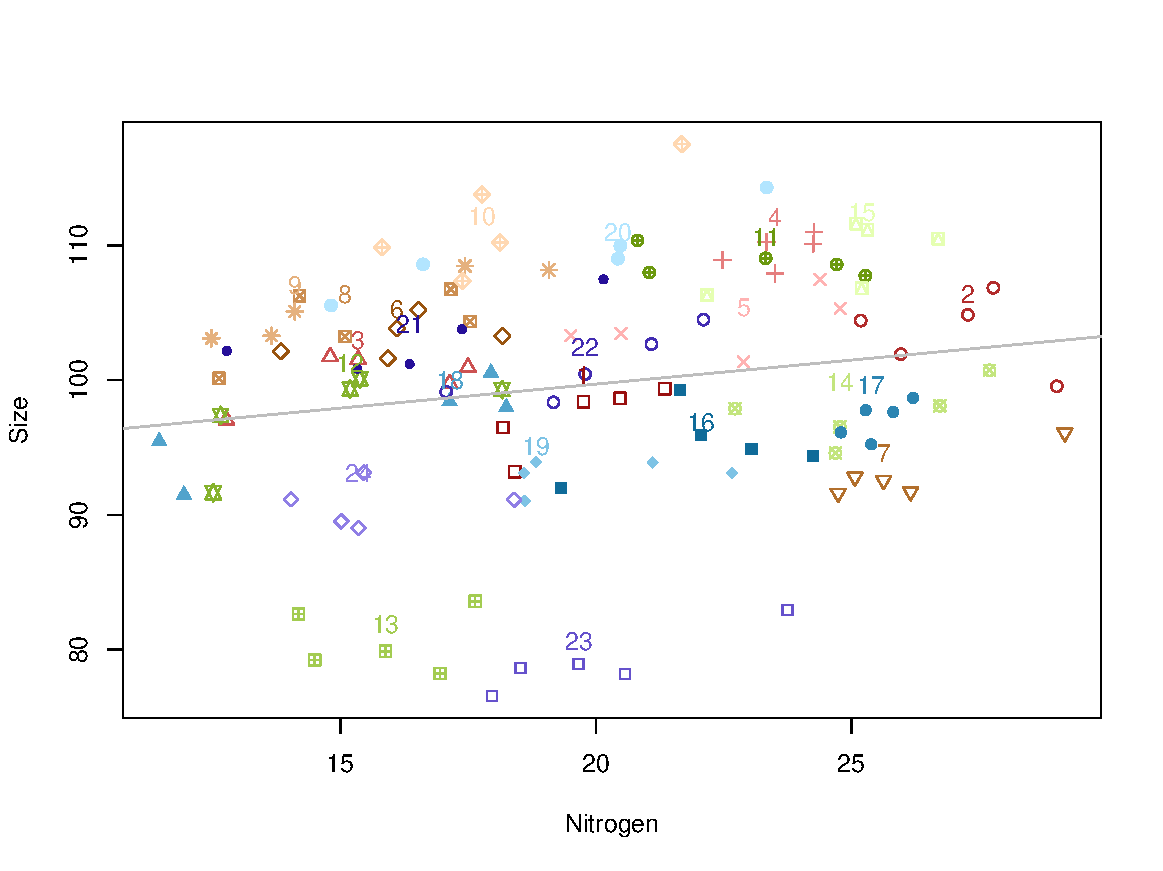
\includegraphics[scale=0.5]{Kap3/hlrm_ols_farms.pdf}
    \caption{Scatter plot of plant size against soil nitrogen concentration across 24 farms, with the global ordinary least squares fit.}
    \label{fig:hlrm_ols_farms}
\end{figure}


The results in Table~\ref{tab:goodness} highlight the trade-off between 
statistical accuracy and computational efficiency across inference methods. 
MCMC clearly outperforms both VI and SVI in terms of predictive adequacy, 
as reflected by substantially lower WAIC and DIC values, a smaller mean squared 
error (MSE), and an $R^2$ close to 1, indicating excellent fit. In contrast, 
the variational methods (VI and SVI) yield considerably poorer predictive 
performance, with WAIC and DIC values more than double those of MCMC, high MSE, 
and almost no explanatory power according to $R^2$.  

\vspace{0.5cm}

However, these improvements in accuracy come at a high computational cost: 
MCMC requires over 500 seconds of runtime, compared to roughly 55 seconds 
for both VI and SVI. This gap illustrates the typical precision–scalability 
trade-off in Bayesian computation: while MCMC provides reliable posterior 
estimates, it is less scalable to large or streaming datasets, where faster 
but approximate methods such as VI and SVI may be preferable despite their 
loss of accuracy. 

\begin{table}[ht]
\centering
\caption{Count of farm-specific $95\%$ credible intervals (CIs) containing zero for regression coefficients and variances under MCMC, VI, and SVI.}
\label{tab:ic_metodos}
\begin{tabular}{lccc}
\toprule
 & \textbf{MCMC} & \textbf{VI} & \textbf{SVI} \\
\midrule
$\beta_{1j}$   & $0/24$ & $0/24$ & $0/24$ \\
$\beta_{2j}$   & $1/24$ & $0/24$ & $0/24$ \\
$\sigma^{2}_{j}$ & $0/24$ & $0/24$ & $0/24$ \\
\bottomrule
\end{tabular}
\end{table}

\vspace{0.5cm}

Table~\ref{tab:ic_metodos} summarizes the number of credible intervals that include zero across farms for the regression coefficients and error variances. The results indicate that almost no intervals contain zero, with the only exception being $\beta_{2j}$ under MCMC in one farm. This finding is consistent with the strong signal observed in previous analyses, where nitrogen concentration showed a clear positive effect on plant size (Figure~\ref{fig:hlrm_ols_farms}) and predictive distributions concentrated around the global mean (Figure~\ref{fig:hlrm_y_density_farms}).

\begin{figure}[H]
    \centering
    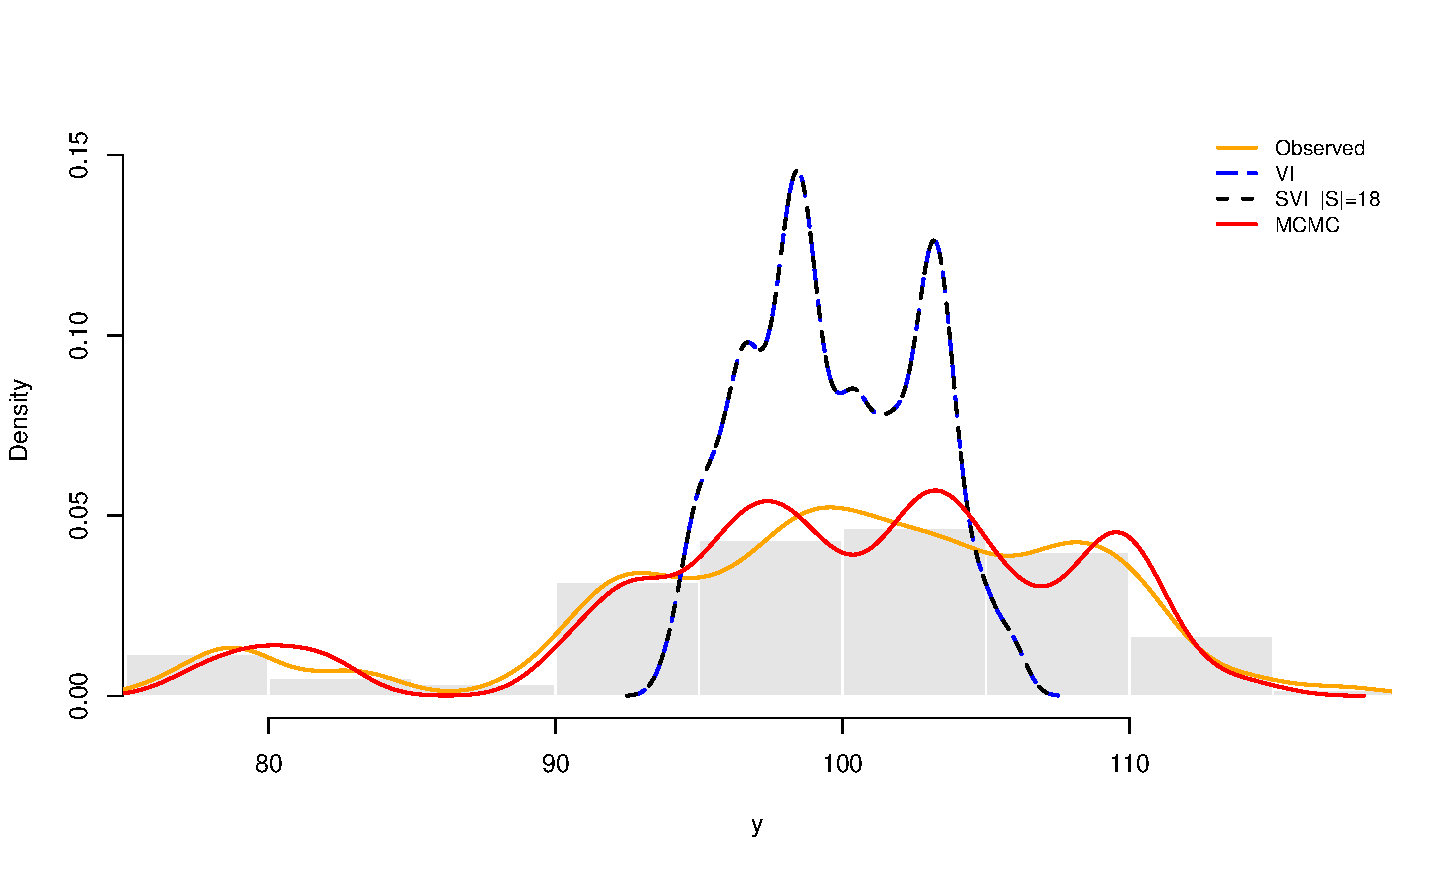
\includegraphics[scale=0.5]{Kap3/hlrm_y_density_farms.pdf}
    \caption{Posterior prediction density of plant size compared across methods.}
    \label{fig:hlrm_y_density_farms}
\end{figure}


An additional consideration is that the mean–field assumption underlying VI and SVI treats the regression coefficients and variance components as independent. This factorization simplifies computations but may overlook structural dependencies or correlations captured by MCMC. As a result, the variational methods can lose part of the joint posterior information, which may explain both the wider intervals for $\beta_{j,1}$ and the reduced sensitivity to farm-specific heterogeneity compared to MCMC.


\begin{table}[!h]
\centering
\caption{\label{tab:PPvalsHLRM}Posterior predictive $p$-values for HLRM (1000 replications), farms dataset.}
\centering
\begin{tabular}[t]{lrrrrrr}
\toprule
\textbf{Method} & \textbf{min} & \textbf{max} & \textbf{IQR} & \textbf{mean} & \textbf{median} & \textbf{sd} \\
\midrule
MCMC & 0.49 & 0.22 & 0.23 & 0.49 & 0.49 & 0.53\\
VI & 0.00 & 1.00 & 1.00 & 0.48 & 0.47 & 1.00\\
SVI & 0.00 & 1.00 & 1.00 & 0.47 & 0.46 & 1.00\\
\bottomrule
\end{tabular}
\end{table}

\newpage

Table~\ref{tab:PPvalsHLRM} reports the posterior predictive $p$-values for the hierarchical linear regression model fitted to the farms dataset. Under MCMC, the distribution of $p$-values appears well-calibrated, with values centered around 0.49 and moderate dispersion (sd = 0.53), suggesting an adequate fit that reflects both central and extreme features of the data. In contrast, both VI and SVI display degenerate behavior, with minimum and maximum values equal to 0 and 1, and an interquartile range (IQR) of 1.0. This indicates that the variational approximations are overly concentrated, yielding posterior predictive distributions that fail to capture the tails of the empirical distribution.  

\vspace{0.5cm}

The inflated posterior predictive $p$-values observed under VI and SVI are a direct consequence of the shrinkage effect introduced by the mean–field approximation. By pulling estimates toward the global mean, variational inference reduces variability and underrepresents extreme observations in the dataset. As a result, measures based on the extremes (min, max, and IQR) are poorly captured, highlighting the limitations of variational methods for fully characterizing uncertainty in hierarchical structures.

\vspace{0.5cm}

Figures~\ref{fig:hlrm_betas_pairs_farms} and \ref{fig:hlrm_sigma2j_farms} present the posterior estimates for the farm-specific intercepts, slopes, and error variances under MCMC, VI, and SVI. The most notable differences between methods appear in the intercepts $\beta_{j,1}$, where the variational approaches tend to produce wider credible intervals. In most cases, the variational intervals contain those obtained by MCMC, reflecting a conservative approximation. This pattern is consistent with the shrinkage effect observed in the predictive density results (Figure~\ref{fig:hlrm_y_density_farms}), where posterior mass accumulated around the global mean. 

\vspace{0.5cm}

Notably, the variational methods (VI and SVI) produce slightly wider intervals, as discussed earlier, but still avoid including zero, which suggests that the main direction of the effect is robust across inference methods. The difference lies in the treatment of uncertainty: while MCMC more accurately captures posterior variability, VI and SVI, due to their mean–field approximation, may underestimate potential dependencies and therefore simplify the structure of the credible intervals.

\vspace{0.5cm}

Figure~\ref{fig:hlrm_sigma2j_farms} presents the posterior means and 95\% credible intervals of the farm-specific error variances under MCMC, VI, and SVI. A systematic pattern is observed: while the posterior means of VI and SVI remain closely aligned with those of MCMC, their credible intervals are consistently wider. This inflation of uncertainty is a direct consequence of the mean–field factorization, which forces independence between regression coefficients and variance parameters, thereby discarding posterior correlations that MCMC naturally captures. As a result, the additional variability observed in VI and SVI should not be interpreted as genuine posterior uncertainty, but rather as an artifact of the variational approximation.  

\newpage

\begin{landscape}
\begin{figure}[H]
    \centering
    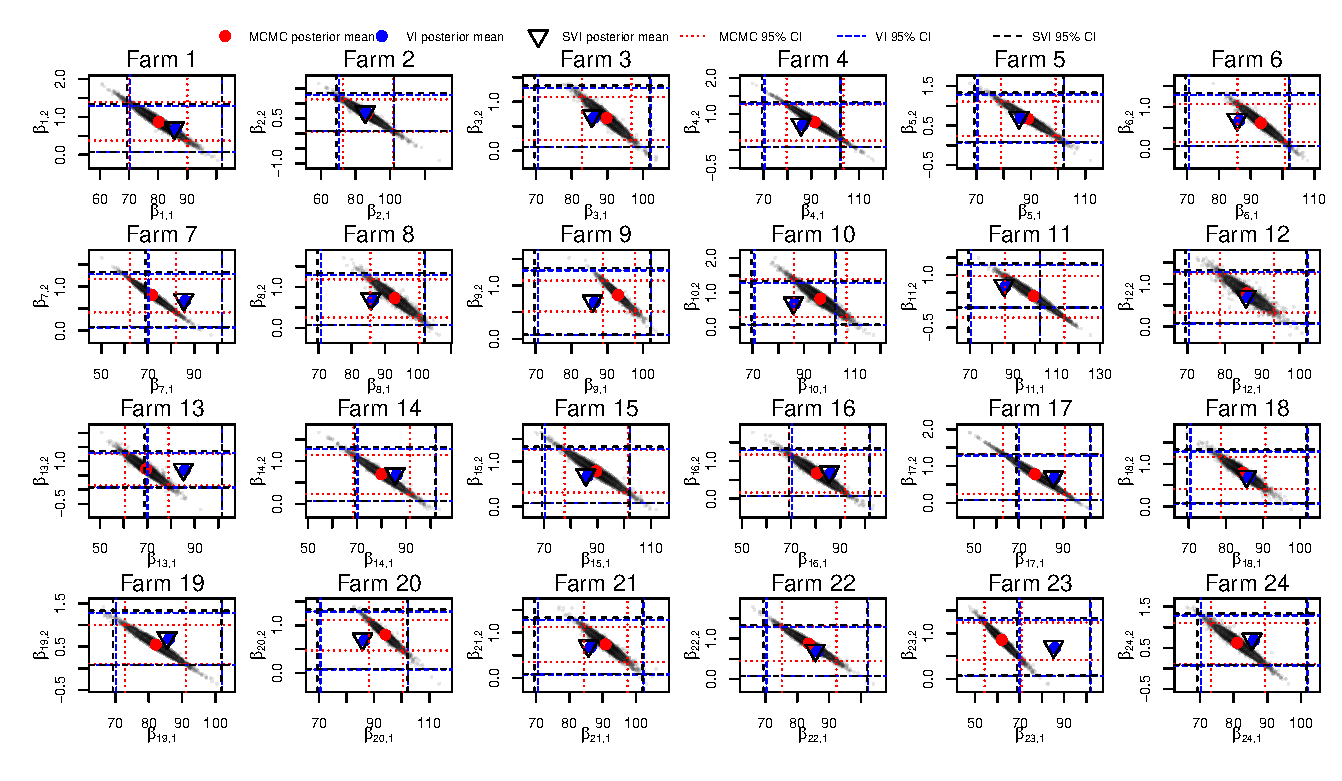
\includegraphics[scale=0.95]{Kap3/hlrm_betas_pairs_farms.pdf}
    \caption{Posterior means and 95\% credible intervals for farm-specific regression coefficients, comparing MCMC, VI, and SVI with $|S|=18$.}
    \label{fig:hlrm_betas_pairs_farms}
\end{figure}
\end{landscape}


\newpage
\begin{landscape}
\begin{figure}[H]
    \centering
    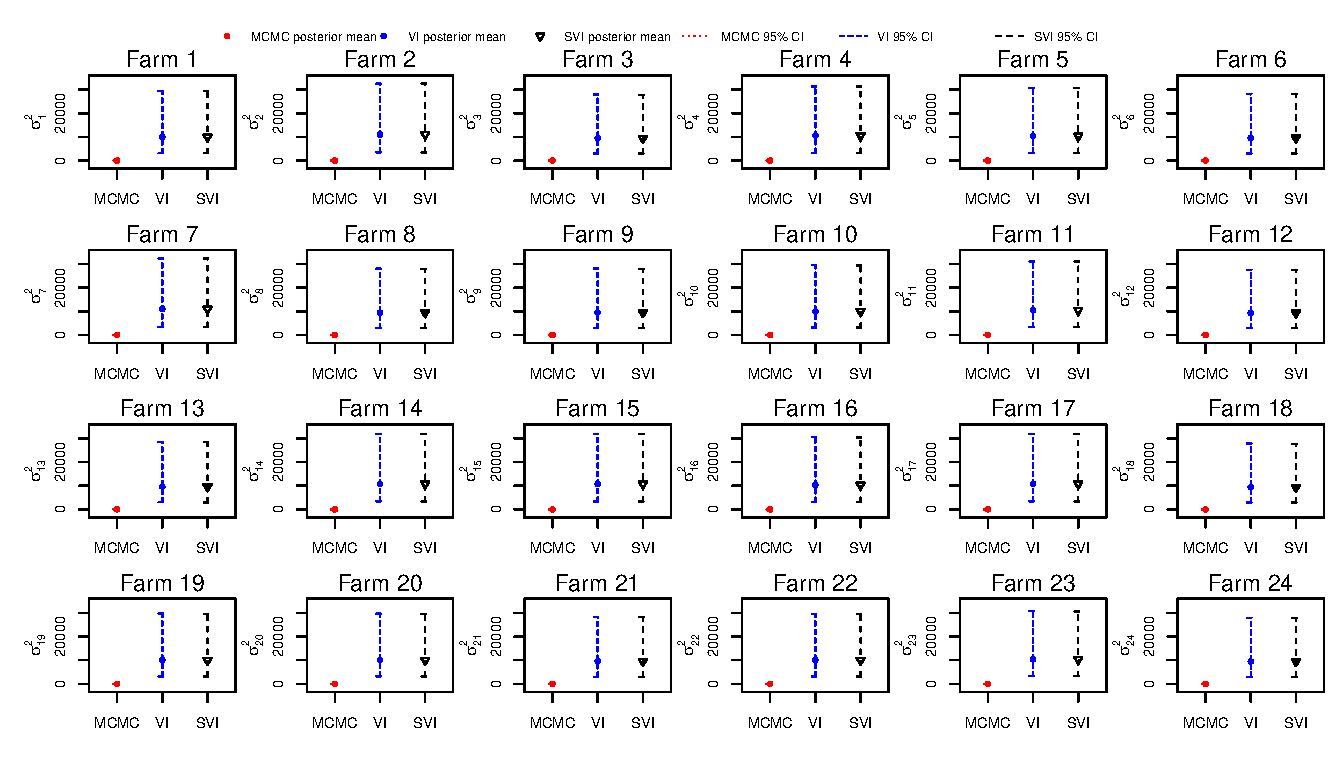
\includegraphics[scale=1]{Kap3/hlrm_sigma2j_farms.pdf}
    \caption{Posterior means and 95\% credible intervals for farm-specific error variances, comparing MCMC, VI, and SVI with $|S|=18$.}
    \label{fig:hlrm_sigma2j_farms}
\end{figure}
\end{landscape}

\begin{landscape}
\begin{figure}[H]
    \centering
    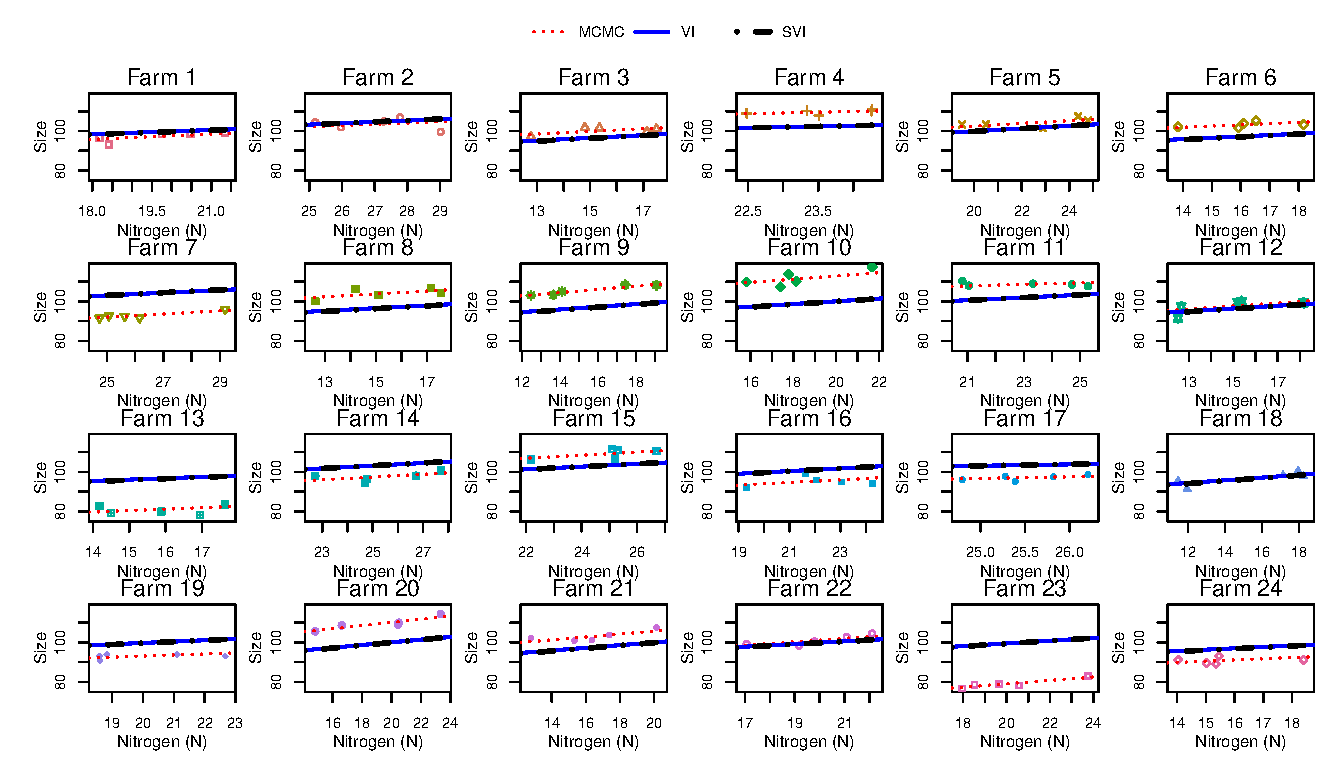
\includegraphics[scale=0.95]{Kap3/hlrm_lines_farms.pdf}
        \caption{Posterior regression lines of plant size on soil nitrogen concentration across farms, comparing MCMC, VI, and SVI with $|S|=18$.}
    \label{fig:hlrm_lines_farms}
\end{figure}
\end{landscape}

This behavior propagates into the regression lines displayed in Figure~\ref{fig:hlrm_lines_farms}. Across most farms, the three methods produce very similar fits, confirming that the dominant nitrogen effect is recovered regardless of the inference strategy. However, in some farms (e.g., 7, 10, 20, and 23), the lines obtained with SVI deviate slightly from those of MCMC and VI. These discrepancies stem from the larger credible intervals associated with the regression coefficients under SVI, which generate more dispersed predictions at the group level. Critically, this highlights a key trade-off: whereas MCMC preserves the full posterior dependence structure and provides more precise local inference, VI and SVI deliver faster approximations at the expense of overestimated variances and a loss of granularity in group-specific effects. Consequently, variational methods may suffice for global predictive purposes, but they are less reliable for fine-grained inference where local parameter dependence is essential.

\section{Clustering Hierarchical Normal Linear Regression Model}

As stated by  \cite{SOSA} an extension of Hierarchical Normal Linear Regression is use the model to capture existing but not explicit defined group structures changing the task of model the response for clustering task with the idea of generate clustering of the hierarchical levels thought as natural clusters and including all its individuals within itself in the cluster of clusters, specifyng the model like Gaussian Mixture to be able of capture this estructure mentioned before.


\vspace{0.5cm}

\cite{SOSA} propose specify the model relaxing the normal assumption representing the response as a finite Gaussian Mixture as follows:

\begin{equation}
\label{CHRLM}
y_{ij} \mid \bm{x}_{ij}, \lbrace\bm{\beta}_k\rbrace, \lbrace\sigma_k^2 \rbrace \stackrel{\text { ind }}{\sim} \sum_{k=1}^{K}\omega_k\mathsf{N}\left(y_{ij}\mid\bm{x}_{ij}^{\bm{\top}} \bm{\beta}_k, \sigma_k^2\right), \quad i=1, \ldots, n_j, \quad j=1, \ldots, m
\end{equation}

where $K$ is a positive fixed integer that represents the number of clusters, $\bm{\beta}_1\cdots\bm{\beta}_K$ and $\sigma^2_1\cdots\sigma^2_K$ are the cluster-specific regression parameters and the cluster-specific variances of the mixture, and $\omega_1,\cdots,\omega_K$ are the mixture probabilities satisfying $\sum_{k=1}^{K}\omega_k=1\text{ and }0<\omega_k<1$.

\vspace{0.5cm}

Another way of expressing the model in \ref{CHRLM} is reparametrize the model by assuming that $P(\gamma_j=k)=\omega_k\text{ for   }j=1, \ldots, m\text{ and }k=1, \ldots, K$ where $\gamma_j$ is a categorical variable that denotes the cluster assignment and takes values $k=1, \ldots, K$ with probabilities $\omega_1,\cdots,\omega_K$. So that the model in \ref{CHRLM} can be written as follows:

\begin{equation}
\label{CHRLM2}
y_{ij} \mid \bm{x}_{ij}, \gamma_j,\bm{\beta}_{\gamma_j},\sigma_{\gamma_j}^2\stackrel{\text { ind }}{\sim} \mathsf{N}\left(y_{ij}\mid\bm{x}_{ij}^{\bm{\top}} \bm{\beta}_{\gamma_j}, \sigma_{\gamma_j}^2\right), \quad i=1, \ldots, n_j, \quad j=1, \ldots, m
\end{equation}

\newpage

\subsection{Prior Distributions}

To continue with Bayesian methodology and propose the prior distributions for model in \ref{CHRLM2}, whit parameters vector $\bm{\Theta}=\left(\gamma, \bm{\omega}, \bm{\zeta}, \bm{\sigma}^2, \bm{\beta}, \bm{\Sigma}, \xi^2\right)$ where $\bm{\gamma}=\left(\gamma_1, \ldots, \gamma_m\right), \bm{\omega}=\left(\omega_1, \ldots, \omega_K\right), \bm{\zeta}=\left(\bm{\beta}_1, \ldots, \bm{\beta}_K\right), \bm{\sigma}^{\mathbf{2}}=\left(\sigma_1^2, \ldots, \sigma_K^2\right)$ represented by figure \ref{fig:DAG_CHLRM}, as follows:

\begin{equation}
    \label{hyper_CHRLM_1}
    \gamma\left|\bm{\omega} \sim \mathsf{Cat}(\bm{\omega}), \quad \bm{\beta}_k\right| \bm{\beta}, \bm{\Sigma} \stackrel{\mathsf{iid}}{\sim} \mathsf{N_p}(\bm{\beta}, \bm{\Sigma}) \quad \text { and } \quad \sigma_k^2 \mid \xi^2 \stackrel{\mathsf{iid}}{\sim} \mathsf{IG}\left(\nu_0 / 2, \nu_0 \xi^2 / 2\right)    
\end{equation}

\begin{equation}
    \label{hyper_CHRLM_2}
    \bm{\omega} \sim \mathsf{Dir}\left(\bm{\alpha}_0\right), \quad \bm{\beta} \sim \mathsf{N_p}\left(\bm{\mu}_0, \bm{\Lambda}_0\right), \quad \bm{\Sigma} \sim \mathsf{IW}\left(n_0, \mathbf{S}_0^{-1}\right), \quad \xi^2 \sim \mathsf{G}\left(a_0, b_0\right)
\end{equation}

with  $\bm{\mu}_0, \bm{\Lambda}_0, n_0, \mathbf{S}_0, \nu_0, a_0, b_0 \text { and } \bm{\alpha}_0$ the hyperparameters of model.

\begin{figure}[H]
    \centering
    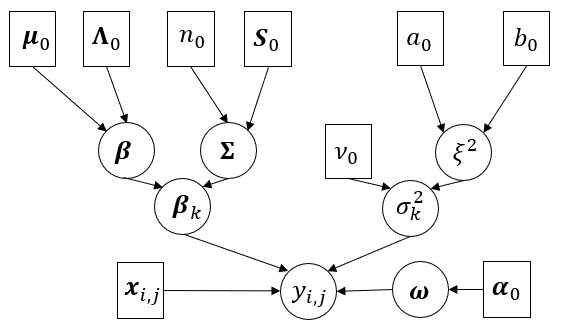
\includegraphics[scale=0.7]{Kap2/DAG_CHLRM.png}
    \caption{DAG Representation CHLRM}
    \label{fig:DAG_CHLRM}
\end{figure}

\subsubsection{Prior Elicitation}
To follow the prior elicitation strategy adopted in the previous models, we set the hyperparameters as follows. For the global regression coefficients $\bm{\beta}$, we set the prior mean as $\bm{\mu}_0 = \hat{\bm{\beta}}_{\text{OLS}}$ and the prior precision as $\bm{\Lambda}_0 = g\,\hat{\sigma}^2_{\text{OLS}}(\bm{X}^\top\bm{X})^{-1}$, where $g = \sum_{j=1}^{m} n_j$ is the total sample size. For the covariance matrix $\bm{\Sigma}$ of the cluster-level effects, we use an Inverse Wishart prior with degrees of freedom $n_0 = p + 2$ and scale matrix $\bm{S}_0 = \bm{\Lambda}_0$, inducing shrinkage consistent with the prior for $\bm{\beta}$. Each cluster-specific variance $\sigma_k^2$ is given an Inverse Gamma prior with shape $\nu_0 = 1$ and scale depending on $\xi^2$, which itself follows a Gamma prior with hyperparameters $a_0 = 1$ and $b_0 = 1/\hat{\sigma}^2_{\text{OLS}}$, allowing control over the overall variance level. Finally, the mixture weights $\bm{\omega}$ follow a Dirichlet prior with concentration parameters $\bm{\alpha}_0 = (1/K, \dots, 1/K)$, resulting in a diffuse prior that does not favor any particular cluster a priori.

\newpage

\subsection{Posterior Inference}

\subsubsection{Gibbs Sampling}

In the CHLRM framework, posterior inference will be conducted via Gibbs sampling. This allows for a straightforward sequential updating of group allocations, mixture proportions, cluster-specific parameters, and global-level variables, ultimately producing approximate samples from the joint posterior distribution, given by:

\begin{equation}
    \label{POST_CHLRM}
    \begin{split}
    p(\bm{\Theta} \mid\bm{y}, \bm{X}) 
&\propto p(\bm{y} \mid \bm{X}, \bm{\gamma}, \bm{\zeta}, \bm{\sigma}^2) 
\, p(\bm{\gamma} \mid \bm{\omega}) 
\, p(\bm{\omega}) 
\, p(\bm{\xi} \mid\bm{\beta},\bm{\Sigma}) \, p(\bm{\beta}) 
p(\bm{\Sigma}) 
\, p(\bm{\sigma}^2 \mid \xi^2) 
\, p(\xi^2)\\
&\propto \prod_{k=1}^{K}\prod_{j=1}^{m} \prod_{i=1}^{n_j} \mathsf{N}(y_{ij}\mid\bm{x}_{ij}^\top \bm{\beta}_{\gamma_j},\sigma_{\gamma_j}^2)^{[\gamma_j = k]}\times\prod_{j=1}^{m}\mathsf{Cat}(\gamma_j\mid\bm{\omega})\times\mathsf{Dir}(\bm{\omega}\mid\bm{\alpha}_0)\\
&\quad\times\prod_{k=1}^{K}\mathsf{N_p}(\bm{\beta}_k\mid\bm{\beta}, \bm{\Sigma})\times\mathsf{N_p}\left(\bm{\beta}\mid\bm{\mu}_0, \bm{\Lambda}_0\right)\times\mathsf{IW}\left(\bm{\Sigma}\mid n_0, \mathbf{S}_0^{-1}\right)\\
&\quad\times\prod_{k=1}^{K}\mathsf{IG}\left(\sigma_k^2 \mid\nu_0 / 2, \nu_0 \xi^2 / 2\right)\times\mathsf{G}\left(\xi^2 \mid a_0, b_0\right)\\
&\propto \prod_{j=1}^{m} \prod_{i=1}^{n_j} (\sigma_{\gamma_j}^2)^{-1/2} 
\exp\left\{ -\frac{1}{2\sigma_{\gamma_j}^2} (y_{ij} - \bm{x}_{ij}^\top \bm{\beta}_{\gamma_j})^2 \right\}  \times\prod_{j=1}^{m} \prod_{k=1}^{K} \omega_k ^{[\gamma_j = k]}\times\prod_{k=1}^{K}\omega_k^{\alpha_{0k}-1}\\
&\quad \times \prod_{j=1}^{m} |\bm{\Sigma}|^{-1/2} 
\exp\left\{ -\frac{1}{2} (\bm{\beta}_j - \bm{\beta})^\top \bm{\Sigma}^{-1} (\bm{\beta}_j - \bm{\beta}) \right\}  \times \prod_{k=1}^{K} |\bm{\Sigma}|^{-1/2} 
\exp\left\{ -\frac{1}{2} (\bm{\beta}_k - \bm{\mu}_0)^\top \bm{\Sigma}^{-1} (\bm{\beta}_k - \bm{\mu}_0) \right\} \\
&\quad \times |\bm{\Sigma}|^{-(n_0 + p + 1)/2} 
\exp\left\{ -\frac{1}{2} \operatorname{tr}(\bm{S}_0 \bm{\Sigma}^{-1}) \right\}  \times \prod_{j=1}^{m} (\sigma_j^2)^{-\left(\nu_0 / 2 + 1\right)} 
\exp\left\{ -\frac{\nu_0 \xi^2}{2\sigma_j^2} \right\} \times \prod_{j=1}^{m} (\xi^2)^{a_0 - 1} 
\exp\left\{ -b_0 \xi^2 \right\}
\end{split}
\end{equation}

then, the f.c.d.s for this model are:

\begin{itemize}
    \item f.c.d of $\gamma_j$ for $j=1,\cdots,m$.
    
    \begin{equation}
        \label{CHLRM_MCMC_gammaj}
        \gamma_j\mid \text{rest}\sim \mathsf{Cat}\left(\left\lbrace p(\gamma_j = 1 \mid \text{rest}),\dots,p(\gamma_j = K \mid \text{rest}\right) \rbrace\right)
    \end{equation}

    with $p(\gamma_j = k \mid \text{rest}) \propto \omega_k \prod_{i=1}^{n_j} (\sigma_k^2)^{-1/2} 
\exp\left\{ -\frac{1}{2\sigma_k^2} (y_{ij} - \bm{x}_{ij}^\top \bm{\beta}_k)^2 \right\}$

    \item f.c.d of $\bm{\omega}$

    \begin{equation}
    \label{CHLRM_MCMC_Omega}
    \bm{\omega} \mid \text{rest} \sim \mathsf{Dir}(\alpha_{01} + n_1,\,  \dots,\, \alpha_{0K} + n_K)\\
    \end{equation}

with $n_k=\#\left\lbrace j : \gamma_j=k\right\rbrace$

\item f.c.d of $\bm{\beta}_k$ for $k=1,\cdots,K$

\begin{equation}
\label{CHLRM_MCMC_Betak}
\bm{\beta}_k \mid \text{rest} \sim \mathsf{N_p}\left((\sigma_k^{-2}\bm{X}_{k}^\top\bm{X}_{k}+\bm{\Sigma}^{-1})^{-1}(\sigma_k^{-2}\bm{X}_{k}^\top\bm{y}_{k}+\bm{\Sigma}^{-1}\bm{\beta}) , (\sigma_k^{-2}\bm{X}_{k}^\top\bm{X}_{k}+\bm{\Sigma}^{-1})^{-1}\right)
\end{equation}

note that if cluster $k$ is empty, then the f.c.d of $\bm{\beta}_k$ is just $\bm{\beta}_k \mid \text{rest} \sim \mathsf{N_p}(\bm{\beta}, \bm{\Sigma})$, with $\bm{X}_{k} = [\bm{X}_j^\top : \gamma_j = k]^\top$ , where $\bm{X}_j = \left[\bm{x}_{1, j}, \ldots, \bm{x}_{n_j, j}\right]^\top$ a $n_j \times p$ matrix and $\bm{x}_{ij}$ is a $p \times 1$ vector of regressors for observation $i$ in group $j$ and $\bm{y}_{k} = [\bm{y}_j^\top : \gamma_j = k]^\top$ where $\bm{y}_j = \left[y_{1, j}, \ldots, y_{n_j, j}\right]^\top$  is a $n_j \times 1$ vector of response variable values for group $j$.

\item f.c.d of $\sigma_k^2$ for $k=1,\cdots,K$

\begin{equation}
\label{CHLRM_MCMC_sigma2k}
\sigma_k^2 \mid \text{rest} \sim\mathsf{IG} \left( 
\frac{\nu_0 + \sum_{\left\lbrace j : \gamma_j = k\right\rbrace}n_j}{2},\ 
\frac{ \nu_0 \xi^2 + (\bm{y}_{k} - \bm{X}_{k} \bm{\beta}_k)^\top(\bm{y}_{k} - \bm{X}_{k} \bm{\beta}_k) }{2} 
\right)
\end{equation}

note that if cluster $k$ is empty, then the f.c.d of $\sigma_k^2$ is just $\sigma_k^2 \mid \text{rest} \sim\mathsf{IG}\left(\frac{\nu_0}{2},\frac{ \nu_0 \xi^2}{2}\right) $.

\item f.c.d of $\xi^2$

\begin{equation}
\label{CHLRM_MCMC_xi2}
\xi^2 \mid \text{rest} \sim \mathsf{G} \left(
\frac{\kappa \nu_0}{2} + a_0,\ 
\frac{\nu_0}{2} \sum_{\left\lbrace k : n_k > 0\right\rbrace} \sigma_k^{-2} + b_0
\right)
\end{equation}

where $\kappa = \#\left\lbrace k : n_k > 0\right\rbrace$ is the number of non empty clusters.

\item f.c.d of $\bm{\beta}$

\begin{equation}
\label{CHLRM_MCMC_Beta}
\bm{\beta} \mid \text{rest} \sim  \mathsf{N_p}\left(\left( \kappa \bm{\Sigma}^{-1} + \bm{\Lambda}_0^{-1} \right)^{-1}\left( \bm{\Lambda}_0^{-1} \bm{\mu}_0 + \bm{\Sigma}^{-1} \sum_{\left\lbrace k : n_k > 0\right\rbrace} \bm{\beta}_k \right), \left( \kappa \bm{\Sigma}^{-1} + \bm{\Lambda}_0^{-1} \right)^{-1}\right)
\end{equation}

\item f.c.d of $\bm{\Sigma}$

\begin{equation}
\label{CHLRM_MCMC_Sigma}
\bm{\Sigma} \mid \text{rest} \sim \mathsf{IW} \left(
\kappa + n_0,\ 
\left(\bm{S}_0 + \sum_{\left\lbrace k : n_k > 0\right\rbrace} (\bm{\beta}_k - \bm{\beta})(\bm{\beta}_k - \bm{\beta})^\top
\right)^{-1}\right)
\end{equation}


\end{itemize}

\begin{algorithm}[H]
\caption{Gibbs Sampling for CHLRM}
\begin{algorithmic}
\State \textbf{Input} Initial values $\{\gamma_j^{(0)}\}_{j=1}^m$, $\bm{\omega}^{(0)}$, $\{\bm{\beta}_k^{(0)}\}_{k=1}^K$, $\bm{\beta}^{(0)}$, $\bm{\Sigma}^{(0)}$, $\{(\sigma_k^2)^{(0)}\}_{k=1}^K$, $\xi^{2(0)}$, hyperparameters $\bm{\mu}_0, \bm{\Lambda}_0, n_0, \bm{S}_0, a_0, b_0, \nu_0$, data values $\{\bm{y}_j,\bm{X}_j\}_{j=1}^m$
\For{$b = 1, \dots, B$}
  \For{$j = 1, \dots, m$}
    \State Sample $\gamma_j^{(b)} \sim p\!\left(\gamma_j \mid \bm{\omega}^{(b-1)}, \{\bm{\beta}_k^{(b-1)}, (\sigma_k^2)^{(b-1)}\}_{k=1}^K, \bm{y}_j, \bm{X}_j \right)$ from eq.\ref{CHLRM_MCMC_gammaj}
  \EndFor
  \State Sample $\bm{\omega}^{(b)} \sim p\!\left(\bm{\omega} \mid \{\gamma_j^{(b)}\}_{j=1}^m \right)$ from eq.~\ref{CHLRM_MCMC_Omega}
  \For{$k = 1, \dots, K$}
    \State Sample $\bm{\beta}_k^{(b)} \sim p\!\left(\bm{\beta}_k \mid \bm{\beta}^{(b-1)}, \bm{\Sigma}^{(b-1)}, (\sigma_k^2)^{(b-1)}, \{\bm{y}_j, \bm{X}_j, \gamma_j^{(b)}\}_{j=1}^m \right)$ from eq.~\ref{CHLRM_MCMC_Betak}
    \State Sample $(\sigma_k^2)^{(b)} \sim p\!\left(\sigma_k^2 \mid \bm{\beta}_k^{(b)}, (\xi^2)^{(b-1)}, \{\bm{y}_j, \bm{X}_j, \gamma_j^{(b)}\}_{j=1}^m \right)$ from eq.~\ref{CHLRM_MCMC_sigma2k}
  \EndFor
  \State Sample $\bm{\beta}^{(b)} \sim p\!\left(\bm{\beta} \mid \{\bm{\beta}_k^{(b)}\}_{k=1}^K, \bm{\Sigma}^{(b-1)} \right)$ from eq.~\ref{CHLRM_MCMC_Beta}
  \State Sample $\bm{\Sigma}^{(b)} \sim p\!\left(\bm{\Sigma} \mid \{\bm{\beta}_k^{(b)}\}_{k=1}^K, \bm{\beta}^{(b)} \right)$ from eq.~\ref{CHLRM_MCMC_Sigma}
  \State Sample $(\xi^2)^{(b)} \sim p\!\left(\xi^2 \mid \{(\sigma_k^2)^{(b)}\}_{k=1}^K \right)$ from eq.~\ref{CHLRM_MCMC_xi2}
\EndFor
\State \textbf{Output} Draws $\{\gamma_j^{(b)},\bm{\omega}^{(b)},\bm{\beta}_k^{(b)},(\sigma_k^2)^{(b)},\bm{\beta}^{(b)},\bm{\Sigma}^{(b)},(\xi^2)^{(b)}\}_{b=1}^B$
\end{algorithmic}
\end{algorithm}


For detailed and explicit derivations of these results, see Appendix \ref{Appendix_B}.

\subsubsection{CAVI}

As before, we specify a variational distribution to approximate the posterior distribution under the mean--field assumption described in result \ref{MFA}. Leveraging the CAVI framework for conditionally conjugate models presented in \ref{NMVFB_opt}, we derive the update rules for each variational factor in the CHLRM. It is important to highlight that these variational factors naturally decompose into local parameters, which are specific to each group assignment variable and its associated cluster-level effects, and global parameters, which correspond to latent variables shared across all clusters.

\begin{equation}
\label{Q_CHLRM}
\begin{split}
q(\bm{\Theta})&=\prod_{k=1}^{K}q(\bm{\beta}_k)q(\bm{\beta})q(\bm{\Sigma})\prod_{k=1}^{K}q(\sigma_k^2)q(\xi^2)\prod_{j=1}^{m}q(\gamma_j)q(\bm{\omega})\\
&= \left(q(\bm{\omega})q(\bm{\beta})q(\bm{\Sigma})q(\xi^2)\prod_{k=1}^{K}q(\bm{\beta}_k)q(\sigma_k^2)\right)\left(\prod_{j=1}^{m}q(\gamma_j)\right)
\end{split}
\end{equation}

\begin{itemize}
    \item Factor  $q(\gamma_j)=\mathsf{Cat}(\lbrace{\rho_{j1},\dots,\rho_{jK}\rbrace})$, with

\begin{equation}
\label{CHLRM_CAVI_rhojk_gamma}
\log \rho_{jk} \propto -\tfrac{n_j}{2}\mathsf{E}_{\sigma^2_k}\left[\log\sigma^2_{k}\right]
-\tfrac{1}{2}\mathsf{E}_{\sigma^2_k}\left[\frac{1}{\sigma^2_{k}}\right]\mathsf{E}_{\bm{\beta}_k}\left[\left(\bm{y}_{j}-\bm{X}_{j}\bm{\beta}_{k}\right)^\top\left(\bm{y}_{j}-\bm{X}_{j}\bm{\beta}_{k}\right)\right]+\mathsf{E}_{\omega}\left[\log\omega_k\right]
\end{equation}

\item Factor $q(\bm{\omega})=\mathsf{Dir}\left(\left\lbrace \alpha_{\bm{\omega}1},\dots,\alpha_{\bm{\omega}K}\right\rbrace\right)$, with

\begin{equation}
    \label{CHLRM_CAVI_Alpha_Omega}
    \alpha_{\bm{\omega}k}=\alpha_{0k}+\sum_{j=1}^{m}\mathsf{E}_{\gamma_j}\left[[\gamma_j=k]\right]
\end{equation}

\item Factor $q(\bm{\beta}_k)=\mathsf{N_p}(\bm{\mu}_{\bm{\beta}_k},\bm{\Sigma}_{\bm{\beta}_k})$, with

\begin{equation}
\label{CHLRM_CAVI_Sigma_Betak}
\bm{\Sigma}_{\bm{\beta}_k}^{-1} = \mathsf{E}_{\sigma^2_k}\left[{\sigma_k}^{-2}\right] \sum_{j=1}^{m}\mathsf{E}_{\gamma_j}\left[[\gamma_j=k\right]]\bm{X}_{j}^\top \bm{X}_{j}  + \mathsf{E}_{\bm{\Sigma}}\left[\bm{\Sigma}^{-1}\right] ,
\end{equation}

\begin{equation}
\label{CHLRM_CAVI_Mu_Betak}
\bm{\mu}_{\bm{\beta}_k}= \bm{\Sigma}_{\bm{\beta}_k}\left[\mathsf{E}_{\sigma^2_k}\left[{\sigma_k}^{-2}\right] \sum_{j=1}^{m}\mathsf{E}_{\gamma_j}\left[[\gamma_j=k\right]]\bm{X}_{j}^\top \bm{y}_{j} + \mathsf{E}_{\bm{\Sigma}}\left[\bm{\Sigma}^{-1}\right] \mathsf{E}_{\bm{\beta}}\left[\bm{\beta} \right] \right]
\end{equation}

\item Factor $q(\bm{\beta})=\mathsf{N_p}(\bm{\mu}_{\bm{\beta}},\bm{\Sigma}_{\bm{\beta}})$, with

\begin{equation}
\label{CHLRM_CAVI_Sigma_Beta}
\bm{\Sigma}_{\bm{\beta}} = \left[\bm{\Lambda}_0^{-1}   + \sum_{k=1}^{K}\mathsf{E}_{\bm{\Sigma}}\left[\bm{\Sigma}^{-1}\right]  \right] ^{-1},
\end{equation}

\begin{equation}
\label{CHLRM_CAVI_Mu_Beta}
\bm{\mu}_{\bm{\beta}}= \left[\bm{\Lambda}_0^{-1}   + \sum_{k=1}^{K}\mathsf{E}_{\bm{\Sigma}}\left[\bm{\Sigma}^{-1}\right]  \right]^{-1}\left[\bm{\Lambda}_0^{-1} \bm{\mu}_0 + \sum_{k=1}^{K}\mathsf{E}_{\bm{\Sigma}}\left[\bm{\Sigma}^{-1}\right] \mathsf{E}_{\bm{\beta}_k}\left[\bm{\beta}_k \right]\right]
\end{equation}

\item Factor $q(\bm{\Sigma})=\mathsf{IW}(\nu_{\bm{\Sigma}},\bm{S}_{\bm{\Sigma}}^{-1})$, with

\begin{equation}
\label{CHLRM_CAVI_nu_Sigma}
\nu_{\bm{\Sigma}} = n_0+K,
\end{equation}

\begin{equation}
\label{CHLRM_CAVI_S_Sigma}
\bm{S}_{\bm{\Sigma}}=  \bm{S}_0 + \sum_{k=1}^{K} \mathsf{E}_{\bm{\beta}_k,\bm{\beta}}\left[\left(\bm{\beta}_k - \bm{\beta})(\bm{\beta}_k - \bm{\beta}\right)^\top\right]
\end{equation}

\item Factor $q(\sigma_k^2)=\mathsf{IG}(a_{\sigma_k^2},b_{\sigma_k^2})$, with

\begin{equation}
\label{CHLRM_CAVI_a_sigma2k}
a_{\sigma_k^2}= \frac{\nu_0 + \sum_{j=1}^{m}\mathsf{E}_{\gamma_j}\left[[\gamma_j=k]\right]n_j}{2},
\end{equation}

\begin{equation}
\label{CHLRM_CAVI_b_sigma2k}
b_{\sigma_k^2}= \frac{ \nu_0 \mathsf{E}_{\xi^2}\left[\xi^2\right] +  \sum_{j=1}^{m}\mathsf{E}_{\gamma_j}\left[[\gamma_j=k]\right]\mathsf{E}_{\bm{\beta}_k}\left[\left(\bm{y}_{j} - \bm{X}_{j} \bm{\beta}_k)^\top(\bm{y}_{j} - \bm{X}_{j} \bm{\beta}_k\right)\right]}{2}
\end{equation}

\item Factor $q(\xi^2)=\mathsf{G}(a_{\xi^2},b_{\sigma_j^2})$, with

\begin{equation}
\label{CHLRM_CAVI_a_xi2}
a_{\xi^2}=  a_0 +\sum_{k=1}^{K}\frac{\nu_0}{2},
\end{equation}

\begin{equation}
\label{CHLRM_CAVI_b_xi2}
b_{\xi^2}= b_0 + \frac{\nu_0}{2} \sum_{k=1}^{K} \mathsf{E}_{\sigma^2_k}\left[\sigma_k^{-2}\right]
\end{equation}

\item ELBO $\mathcal{L}(q(\bm{\Theta}))$

\begin{equation}
\label{CHLRM_CAVI_ELBO}
\begin{split}
\mathcal{L}(q(\bm{\Theta}))
&=\mathsf{E}_{\bm{\Theta}}\left[\log p(\bm{\Theta},\bm{y}, \bm{X})\right]-\mathsf{E}_{\bm{\Theta}}\left[\log q(\bm{\Theta})\right]\\
&= \mathsf{E}_{\bm{\Theta}}\left[\log p(\bm{y}\mid\bm{X},\bm{\gamma},\bm{\zeta},\bm{\sigma}^2)\right] + \sum_{j=1}^{m}\left(\mathsf{E}_{\bm{\Theta}}\left[\log p(\gamma_j\mid\bm{\omega})\right] -\mathsf{E}_{\gamma_j}\left[\log q(\gamma_j)\right]\right) \\
&\quad + \left(\mathsf{E}_{\bm{\Theta}}\left[\log p(\bm{\omega})\right]- \mathsf{E}_{\bm{\omega}}\left[\log q(\bm{\omega})\right]\right)+ \sum_{k=1}^{K}\left(\mathsf{E}_{\bm{\Theta}}\left[\log p(\bm{\beta}_k\mid\bm{\beta},\bm{\Sigma})\right] -\mathsf{E}_{\bm{\beta}_k}\left[\log q(\bm{\beta}_k)\right]\right)\\
&\quad + \left(\mathsf{E}_{\bm{\Theta}}\left[\log p(\bm{\beta})\right]- \mathsf{E}_{\bm{\beta}}\left[\log q(\bm{\beta})\right]\right) + \left(\mathsf{E}_{\bm{\Theta}}\left[\log p(\bm{\Sigma})\right]-\mathsf{E}_{\bm{\Sigma}}\left[\log q(\bm{\Sigma})\right] \right)\\
&\quad + \sum_{k=1}^{K}\left(\mathsf{E}_{\bm{\Theta}}\left[\log p(\sigma_k^2 \mid \xi^2)\right]-\mathsf{E}_{\sigma_k^2}\!\left[\log q(\sigma_k^2)\right]\right) + \left(\mathsf{E}_{\bm{\Theta}}\left[\log p(\xi^2)\right]- \mathsf{E}_{\xi^2}\!\left[\log q(\xi^2)\right]\right) 
\end{split}
\end{equation}

where

\begin{itemize}
    \item 
    $
    \begin{aligned}
       \mathsf{E}_{\bm{\Theta}}\left[\log p(\bm{y}\mid\bm{X},\bm{\gamma},\bm{\zeta},\bm{\sigma}^2)\right]&=\sum_{j=1}^{m}\sum_{k=1}^{K}\Bigg[\rho_{jk}\Bigg(
-\tfrac{n_j}{2}\log(2\pi)
-\tfrac{n_j}{2}\left(\log b_{\sigma_k^2}-\psi(a_{\sigma_k^2})\right) \\
&\qquad
-\tfrac{1}{2}\left(\tfrac{a_{\sigma_k^2}}{b_{\sigma_k^2}}\right)
\Big[
(\bm{y}_j-\mathbf{X}_j\bm{\mu}_{\bm{\beta}_k})^\top(\bm{y}_j-\mathbf{X}_j\bm{\mu}_{\bm{\beta}_k})
+\operatorname{tr}\left(\mathbf{X}_j^\top\mathbf{X}_j\,\bm{\Sigma}_{\bm{\beta}_k}\right)
\Big]
\Bigg)\Bigg] \\ 
    \end{aligned}
    $

    \item 
    $
    \mathsf{E}_{\bm{\Theta}}\left[\log p(\gamma_j\mid\bm{\omega})\right]=\sum_{k=1}^{K}\rho_{jk}
\Bigg[
\psi\left(\alpha_{0k}+\sum_{j=1}^{m}\rho_{jk}\right) -\psi\left(\sum_{k=1}^{K}\left[\alpha_{0k}+\sum_{j=1}^{m}\rho_{jk} \right]\right)
\Bigg]
    $

    \item 
    $
      \mathsf{E}_{\gamma_j}\left[\log q(\gamma_j)\right]=\sum_{k=1}^{K}\rho_{jk}\log\rho_{jk}  
    $

    \item 
    $
        \mathsf{E}_{\bm{\Theta}}\left[\log p(\bm{\omega})\right]=\log\Gamma\left( \sum_{k=1}^{K} \alpha_{0k} \right)-\sum_{k=1}^{K} \log\Gamma\left(\alpha_{0k}\right)+\sum_{k=1}^{K}\left(\alpha_{0k}-1\right)\left[\psi\left(\alpha_{0k}\right) -\psi\left(\sum_{k=1}^{K}\alpha_{0k}\right)\right] 
    $

        \item 
    $
    \begin{aligned}
    \mathsf{E}_{\bm{\omega}}\left[\log q(\bm{\omega})\right]
    &=\log\Gamma\left( \sum_{k=1}^{K} \left[\alpha_{0k}+\sum_{j=1}^{m}\rho_{jk} \right]\right)-\sum_{k=1}^{K} \log\Gamma\left(\alpha_{0k}+\sum_{j=1}^{m}\rho_{jk}\right)\\
        &\quad+\sum_{k=1}^{K}\left(\alpha_{0k}+\sum_{j=1}^{m}\rho_{jk} -1\right)\left[\psi\left(\alpha_{0k}+\sum_{j=1}^{m}\rho_{jk}\right) -\psi\left(\sum_{k=1}^{K}\left[\alpha_{0k}+\sum_{j=1}^{m}\rho_{jk} \right]\right)\right]
    \end{aligned}
    $

        \item

    $
        \begin{aligned}
        \mathsf{E}_{\bm{\Theta}}\left[\log p(\bm{\beta}_k\mid\bm{\beta},\bm{\Sigma})\right]=&
    -\tfrac{p}{2}\log(2\pi)
    -\tfrac{1}{2}\Bigg(
    -\sum_{i=1}^{p}\psi\!\!\left(\tfrac{\nu_{\bm{\Sigma}}+1-i}{2}\right)-p\log 2+\log|\bm{S}_{\bm{\Sigma}}^{-1}|
    \Bigg) \\
    &\qquad
    -\tfrac{1}{2}\operatorname{tr}\left(\bm{S}_{\bm{\Sigma}}^{-1}\!\!\left[
    (\bm{\mu}_{\bm{\beta}_k}-\bm{\mu}_{\bm{\beta}})
    (\bm{\mu}_{\bm{\beta}_k}-\bm{\mu}_{\bm{\beta}})^\top
    +\bm{\Sigma}_{\bm{\beta}_k}+\bm{\Sigma}_{\bm{\beta}}
    \right]\right)\\
        \end{aligned}
    $

        \item

    $
    \mathsf{E}_{\bm{\beta}_k}\left[\log q(\bm{\beta}_k)\right]=-\tfrac{p}{2}\log(2\pi e)-\tfrac{1}{2}\log|\bm{\Sigma}_{\bm{\beta}_k}|
    $

        \item 

    $
    \begin{aligned}
        \mathsf{E}_{\bm{\Theta}}\left[\log p(\bm{\beta})\right]=-\tfrac{p}{2}\log(2\pi)-\tfrac{1}{2}\log|\bm{\Lambda}_0|
-\tfrac{1}{2}\Big[
(\bm{\mu}_{\bm{\beta}}-\bm{\mu}_0)^\top\bm{\Lambda}_0^{-1}(\bm{\mu}_{\bm{\beta}}-\bm{\mu}_0)
+\operatorname{tr}\!\!\left(\bm{\Lambda}_0^{-1}\bm{\Sigma}_{\bm{\beta}}\right)
\Big]
    \end{aligned}
    $

        \item 

    $
    \begin{aligned}
        \mathsf{E}_{\bm{\beta}}\left[\log q(\bm{\beta})\right]=-\tfrac{p}{2}\log(2\pi e)-\tfrac{1}{2}\log|\bm{\Sigma}_{\bm{\beta}}|
    \end{aligned}
    $

            \item 

    $
    \begin{aligned}
\mathsf{E}_{\bm{\Theta}}\left[\log p(\bm{\Sigma})\right] &=
\tfrac{n_0}{2}\log|\bm{S}_0|-\tfrac{n_0 p}{2}\log 2-\log\Gamma_p\!\!\left(\tfrac{n_0}{2}\right)
-\tfrac{n_0+p+1}{2}\Bigg(
-\sum_{i=1}^{p}\psi\!\!\left(\tfrac{\nu_{\bm{\Sigma}}+1-i}{2}\right)-p\log 2+\log|\bm{S}_{\bm{\Sigma}}^{-1}|
\Bigg) \\
&\qquad
-\tfrac{\nu_{\bm{\Sigma}}}{2}\operatorname{tr}\left(\bm{S}_0\,\bm{S}_{\bm{\Sigma}}^{-1}\right)
    \end{aligned}
    $

        \item 

    $
    \begin{aligned}
        \mathsf{E}_{\bm{\Sigma}}\left[\log q(\bm{\Sigma})\right]&=\tfrac{\nu_{\bm{\Sigma}}}{2}\log|\mathbf{S}_{\bm{\Sigma}}|
- \tfrac{\nu_{\bm{\Sigma}} p}{2}\log 2
- \log\Gamma_p\left(\tfrac{\nu_{\bm{\Sigma}}}{2}\right) - \tfrac{\nu_{\bm{\Sigma}}+p+1}{2}\left(
-\sum_{i=1}^{p}\psi\left(\tfrac{\nu_{\bm{\Sigma}}+1-i}{2}\right)-p\log 2+\log|\mathbf{S}_{\bm{\Sigma}}^{-1}|
\right) \\ 
&\quad - \tfrac{\nu_{\bm{\Sigma}}}{2}\operatorname{tr}\left(\mathbf{S}_{\bm{\Sigma}}^2\right)
    \end{aligned}
    $

            \item 

    $
    \begin{aligned}
    \mathsf{E}_{\bm{\Theta}}\left[\log p(\bm{\sigma}_k^2 \mid \xi^2)\right]&=\tfrac{\nu_0}{2}\log\left(\tfrac{\nu_0}{2}\right)
+\tfrac{\nu_0}{2}\left(\psi(a_{\xi^2})-\log b_{\xi^2}\right)-\log\Gamma\left(\tfrac{\nu_0}{2}\right)-\tfrac{\nu_0\sigma^2_0}{2}\left(\tfrac{a_{\xi^2}}{b_{\xi^2}}\right)\left(\tfrac{a_{\sigma_k^2}}{b_{\sigma_k^2}}\right)\\
&\quad -\left(\tfrac{\nu_0}{2}+1\right)\left(\log b_{\sigma_k^2}-\psi(a_{\sigma_k^2})\right)
    \end{aligned}
    $

            \item 

    $
    \begin{aligned}
    \mathsf{E}_{\sigma_k^2}\!\left[\log q(\sigma_k^2)\right]&=-\log b_{\sigma_k^2}-\log\Gamma(a_{\sigma_k^2})+(a_{\sigma_k^2}+1)\psi(a_{\sigma_k^2})-a_{\sigma_k^2}
    \end{aligned}
    $

            \item 

    $
    \begin{aligned}
    \mathsf{E}_{\bm{\Theta}}\left[\log p(\xi^2)\right]=a_0\log b_0-\log\Gamma(a_0)
+(a_0-1)\left(\psi(a_{\xi^2})-\log b_{\xi^2}\right)
-b_0\left(\tfrac{a_{\xi^2}}{b_{\xi^2}}\right)
    \end{aligned}
    $

            \item 

    $
    \begin{aligned}
    \mathsf{E}_{\xi^2}\left[\log q(\xi^2)\right]=\log b_{\xi^2}-\log\Gamma(a_{\xi^2})+(a_{\xi^2}-1)\psi(a_{\xi^2})-a_{\xi^2}
    \end{aligned}
    $

    
\end{itemize}

\end{itemize}


\begin{algorithm}[H]
\caption{CAVI for CHLRM}
\label{CAVI_CHLRM_alg}
\begin{algorithmic}
\State \textbf{Input} Init values $\{\bm{\mu}_{\bm{\beta}_k}^{(0)}, \bm{\Sigma}_{\bm{\beta}_k}^{(0)}\}_{k=1}^K,\;\bm{\mu}_{\bm{\beta}}^{(0)},\bm{\Sigma}_{\bm{\beta}}^{(0)},\nu_{\bm{\Sigma}},\bm{S}_{\bm{\Sigma}}^{(0)},\;a_{\xi^2},\; b_{\xi^2}^{(0)},\;\{a_{\sigma_k^2}^{(0)}, b_{\sigma_k^2}^{(0)}\}_{k=1}^K,\;\{\rho_{jk}^{(0)}\}_{j=1}^m,\;\bm{\alpha}^{(0)}$, hyperparameters $\bm{\mu}_0,\bm{\Lambda}_0,n_0,\bm{S}_0,a_0,b_0,\nu_0$, data values $\{\bm{y}_j,\bm{X}_j\}_{j=1}^m$

\While{ELBO not converged}
  \State \textbf{\textit{Local updates}}
  \For{$j = 1,\dots,m$}
    \State Update $q(\gamma_j)$ setting $\rho_{jk}$ (eq. \ref{CHLRM_CAVI_rhojk_gamma}).
  \EndFor
  \State \textbf{\textit{Global updates}}
  \State Update $q(\bm{\omega})$ setting $\bm{\alpha}_{\bm\omega}$ (eq. \ref{CHLRM_CAVI_Alpha_Omega}).
  \For{$k = 1,\dots,K$}
    \State Update $q(\bm{\beta}_k)$ setting $\bm{\mu}_{\bm{\beta}_k}$ (eq. \ref{CHLRM_CAVI_Mu_Betak}) and $\bm{\Sigma}_{\bm{\beta}_k}$ (eq. \ref{CHLRM_CAVI_Sigma_Betak}).
    \State Update $q(\sigma_k^2)$ setting $a_{\sigma_k^2}$ (eq. \ref{CHLRM_CAVI_a_sigma2k}) and $b_{\sigma_k^2}$ (eq. \ref{CHLRM_CAVI_b_sigma2k}).
  \EndFor
  \State Update $q(\bm{\beta})$ setting $\bm{\mu}_{\bm{\beta}}$ (eq. \ref{CHLRM_CAVI_Mu_Beta}) and $\bm{\Sigma}_{\bm{\beta}}$ (eq. \ref{CHLRM_CAVI_Sigma_Beta}).
  \State Update $q(\bm{\Sigma})$ setting $\bm{S}_{\bm{\Sigma}}$ (eq. \ref{CHLRM_CAVI_S_Sigma}).
  \State Update $q(\xi^2)$ setting $a_{\xi^2}$ (eq. \ref{CHLRM_CAVI_a_xi2}) and $b_{\xi^2}$ (eq. \ref{CHLRM_CAVI_b_xi2})
\EndWhile
\State Calculate ELBO $\mathcal{L}\left(q(\bm{\Theta})\right)$  (eq. \ref{CHLRM_CAVI_ELBO})
\State \textbf{Output} Optimal parameters $
\{\bm{\mu}_{\bm{\beta}_k},\bm{\Sigma}_{\bm{\beta}_k}\}_{k=1}^K,
\bm{\mu}_{\bm{\beta}},\bm{\Sigma}_{\bm{\beta}},\nu_{\bm{\Sigma}},
\bm{S}_{\bm{\Sigma}},
a_{\sigma_k^2}, b_{\sigma_k^2},
a_{\xi^2}, b_{\xi^2},
\{\rho_{jk}\}_{j=1}^m,\bm{\alpha}$
\end{algorithmic}
\end{algorithm}

For detailed and explicit derivations of these updates, see Appendix \ref{Appendix_C}.

\subsubsection{SVI}

In the case of the CHLRM, the conjugacy of the prior structure ensures that the updates of the local variational factors can be obtained in closed form, thus satisfying the conditions required for the application of Stochastic Variational Inference (see subsection \ref{SVI}). Specifically, local parameters are updated through a single CAVI step, while the global parameters are refined by means of Robbins--Monro stochastic approximation, as described in the previous subsection. The resulting procedure leading to the iterative algorithm detailed below in \ref{SVI_CHLRM_alg}.


\subsection{Illustration}
\subsubsection{Simulation}
We assess the performance of MCMC, VI, and SVI under a controlled simulation scenario generated from a clustered hierarchical linear regression model (CHLRM) with $K=3$  latent regression components, $p=3$ covariates (including an intercept), $m=15$ groups, and $n_j=20$ observations per group, with mixing weights  \\  $\bm{\omega}=(0.4,\,0.3,\,0.3)$. The component parameters are set to induce heterogeneous linear effects across clusters:
$$
\bm{\beta}_1=\left(-5,\ 8,\ 3\right)^\top,\quad 
\bm{\beta}_2=\left(10,\ -1,\ -2\right)^\top,\quad
\bm{\beta}_3=\left(35,\ -8,\ -2\right)^\top,
$$
with within–component error variances
$$
\sigma_1^2=16,\qquad \sigma_2^2=9,\qquad \sigma_3^2=4.
$$


\begin{figure}[H]
    \centering
    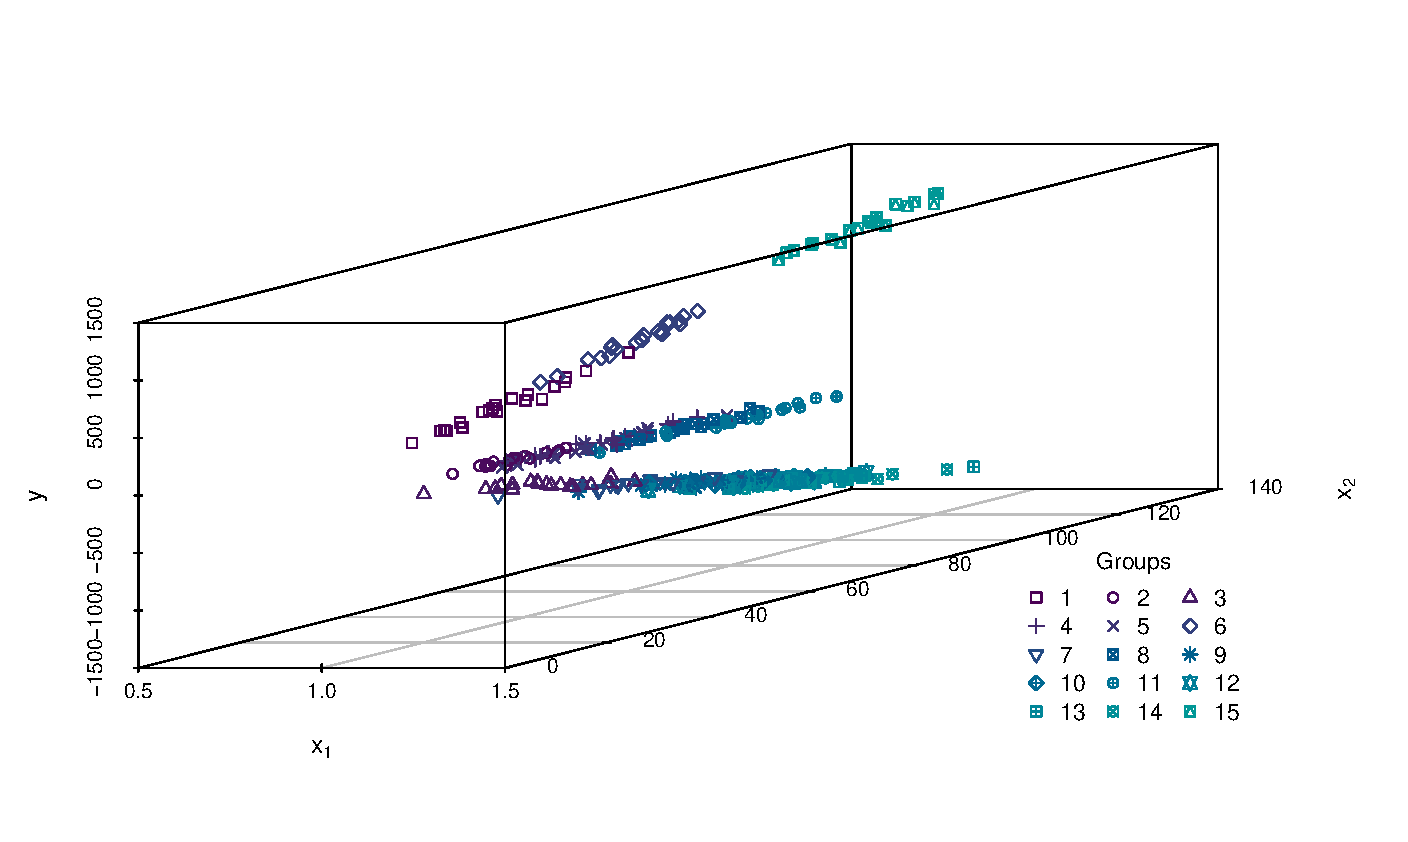
\includegraphics[scale=0.5]{Kap3/chlrm_scatter.pdf}
    \caption{Scatterplot of simulated CHLRM data: response $y$ vs.\ covariates $x_1$ and $x_2$, with group colors.}
    \label{fig:chlrm_scatter}
\end{figure}

Figure~\ref{fig:chlrm_scatter} illustrates the separation of the simulated groups in covariate–response space. This geometric heterogeneity facilitates identifiability of cluster–specific coefficients $(\bm{\beta}_k,\sigma_k^2)$ and underpins the subsequent parameter recovery.


\begin{figure}[H]
    \centering
    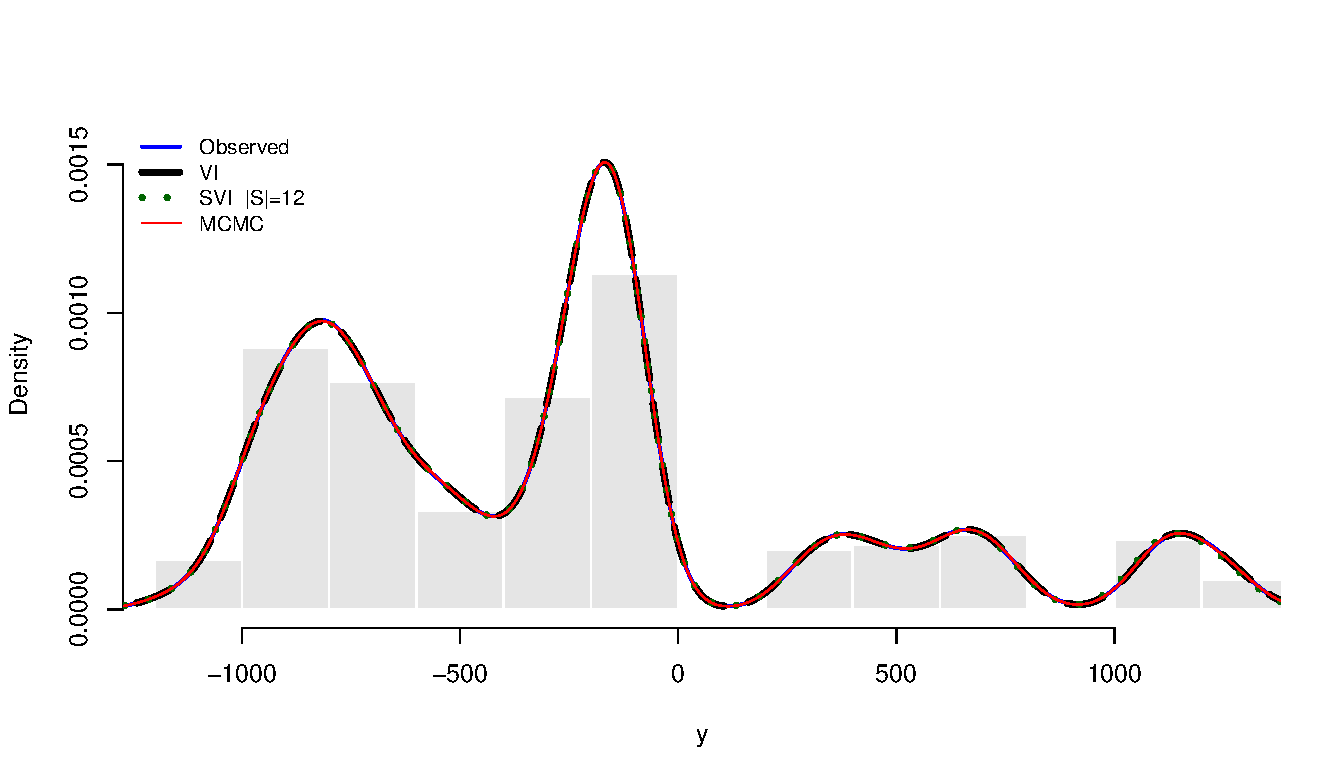
\includegraphics[scale=0.55]{Kap3/chlrm_y_density_sim.pdf}
    \caption{Observed $y$ and posterior predictive densities (MCMC, VI, SVI), simulated data.}
    \label{fig:chlrm_y_density_sim}
\end{figure}

Figure~\ref{fig:chlrm_y_density_sim} shows the multimodal distribution induced by the three regression components. The posterior predictive densities of MCMC, VI, and SVI recover the bulk of the distribution, although VI and SVI display slightly lighter tails, a feature consistent with the mean–field approximation. This predictive fit is consistent with the evidence in Table~\ref{tab:fit_chlrm}, where the MSE and $\mathsf{R}^2$ are broadly comparable across methods. The only notable deviation is the MSE under SVI, which is elevated owing to inflated variability for cluster 1 induced by the mean-field factorization (i.e., the approximation’s neglect of posterior dependencies)..

\begin{figure}[H]
    \centering
    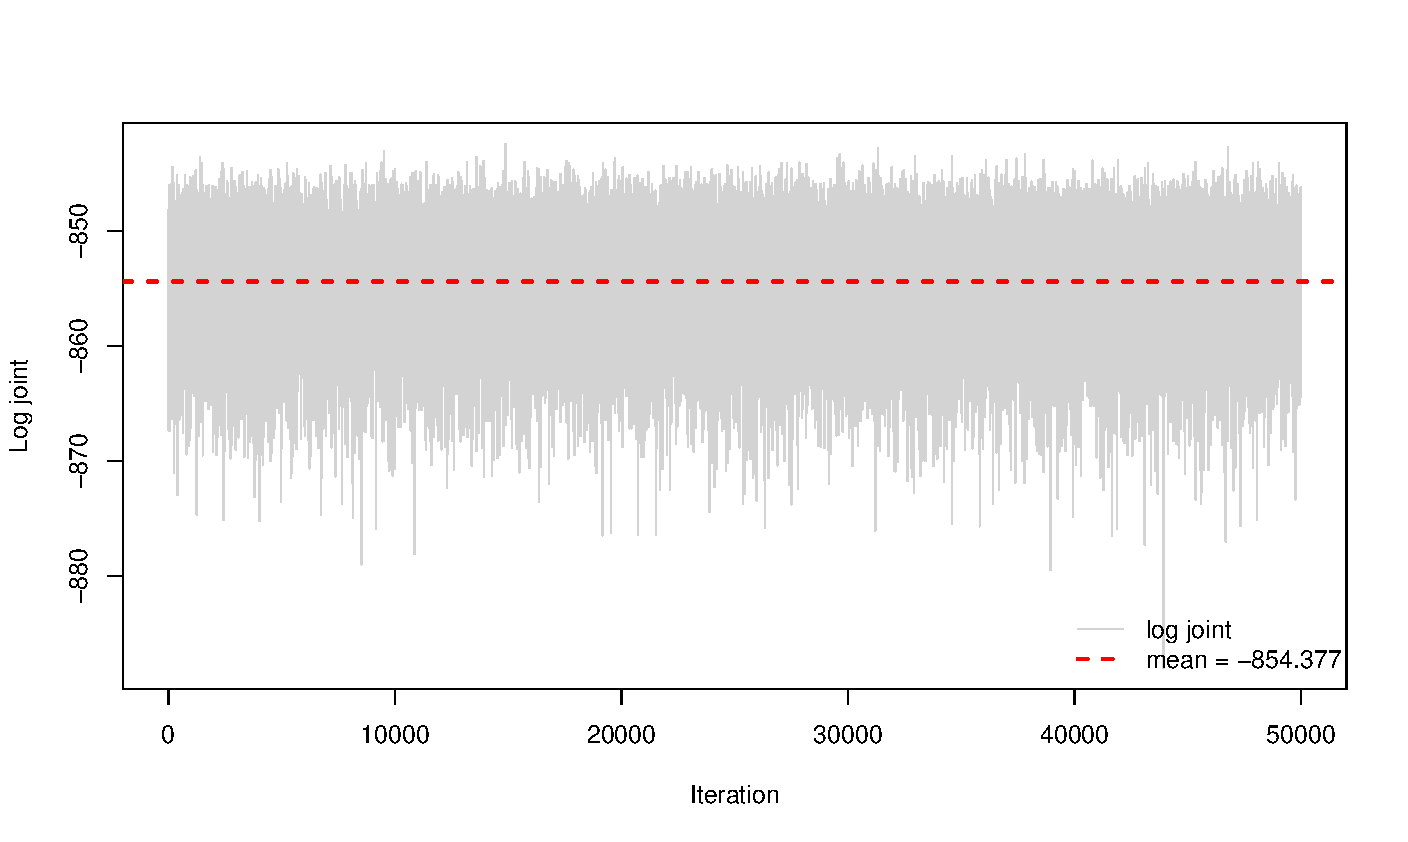
\includegraphics[scale=0.45]{Kap3/chlrm_logjoint_chain.pdf}
    \caption{Trace of the log-joint distribution under MCMC estimation, simulated data.}
    \label{fig:chlrm_logjoint_chain}
\end{figure}

\begin{algorithm}[H]
\scriptsize 
\caption{SVI for CHLRM}
\label{SVI_CHLRM_alg}
\begin{algorithmic}
\State \textbf{Input} Init values $
\{\bm{\mu}_{\bm{\beta}_k}^{(0)},\bm{\Sigma}_{\bm{\beta}_k}^{(0)}\}_{k=1}^K,\;
\bm{\mu}_{\bm{\beta}}^{(0)},\;\bm{\Sigma}_{\bm{\beta}}^{(0)},\;
\nu_{\bm{\Sigma}},\bm{S}_{\bm{\Sigma}}^{(0)},\;
a_{\xi^2}, b_{\xi^2}^{(0)},\;
\{a_{\sigma_k^2}^{(0)}, b_{\sigma_k^2}^{(0)}\}_{k=1}^K,\;
\{\rho_{jk}^{(0)}\}_{j=1}^m,\;
\bm{\alpha}^{(0)}_{\bm{\omega}}$, hyperparameters $\bm{\mu}_0,\bm{\Lambda}_0,n_0,\bm{S}_0,a_0,b_0,\nu_0,\bm{\alpha}_0$, learning rate parameters $\tau,\chi$, minibatch size $|\mathcal{S}|$, number of iterations $T$

\For{$t = 1,\dots,T$}
\State \textbf{\textit{Local updates}}
  \State Select a mini-batch of groups $\mathcal{S} \subset \{1,\dots,m\}$.
  \For{$j \in \mathcal{S}$}
    \State Update $q(\gamma_j)$ setting $\rho_{jk}^{(t)}$ (eq. \ref{CHLRM_CAVI_rhojk_gamma}).
  \EndFor
  \State  Calculate step size  $\rho_t = (t+\tau)^{-\chi}$
  \State \textbf{\textit{Noisy Gradients}}
  \State Calculate Intermediate global parameters
  $$
    \hat{\bm{\Sigma}_{\bm{\beta}_k}}^{-1} =  \mathsf{E}_{\bm{\Sigma}}\left[\bm{\Sigma}^{-1}\right]+\mathsf{E}_{\sigma^2_k}\left[{\sigma_k}^{-2}\right] \tfrac{m}{|\mathcal{S}|}\sum_{j \in \mathcal{S}} \mathsf{E}_{\gamma_j}\left[[\gamma_j=k]\right]\bm{X}_{j}^\top \bm{X}_{j}
  ,\quad
  \hat{\bm{\mu}_{\bm{\beta}_k}} =\hat{\bm{\Sigma}_{\bm{\beta}_k}}\left( \bm{\Lambda}_0^{-1} \bm{\mu}_0 +\tfrac{m}{|\mathcal{S}|}\sum_{j \in \mathcal{S}} \sum_{k=1}^K  \mathsf{E}_{\bm{\Sigma}}\left[\bm{\Sigma}^{-1}\right] \mathsf{E}_{\bm{\beta}_k}\!\left[\bm{\beta}_k \right]\right)
  $$
    $$
    \hat{a_{\sigma^2_k}} =  \frac{\nu_0}{2} + \frac{1}{2}\tfrac{m}{|\mathcal{S}|}\sum_{j \in \mathcal{S}}\mathsf{E}_{\gamma_j}\left[[\gamma_j=k]\right]n_j
  ,\quad
  \hat{b_{\sigma_k^2}} =\frac{ \nu_0 }{2}\mathsf{E}_{\xi^2}\left[\xi^2\right] +  \frac{1}{2}\tfrac{m}{|\mathcal{S}|}\sum_{j \in \mathcal{S}}\mathsf{E}_{\gamma_j}\left[[\gamma_j=k]\right]\mathsf{E}_{\bm{\beta}_k}\left[\left(\bm{y}_{j} - \bm{X}_{j} \bm{\beta}_k\right)^\top\left(\bm{y}_{j} - \bm{X}_{j} \bm{\beta}_k\right)\right]
  $$
    $$
    \hat{\bm{\Sigma}_{\bm{\beta}}}^{-1} = \bm{\Lambda}_0^{-1} + \sum_{k=1}^K 
  \mathsf{E}_{\bm{\Sigma}}\left[\bm{\Sigma}^{-1}\right]
  ,\quad
  \hat{\bm{\mu}_{\bm{\beta}}} =\hat{\bm{\Sigma}_{\bm{\beta}}}\left( \bm{\Lambda}_0^{-1} \bm{\mu}_0 +\sum_{k=1}^K  \mathsf{E}_{\bm{\Sigma}}\left[\bm{\Sigma}^{-1}\right] \mathsf{E}_{\bm{\beta}_k}\!\left[\bm{\beta}_k \right]\right)
  $$
  $$
  \hat{\bm{S}_{\bm{\Sigma}}} = \bm{S}_0+ \sum_{k=1}^K  \mathsf{E}_{\bm{\beta}_k,\bm{\beta}}\!\left[(\bm{\beta}_k-\bm{\beta})(\bm{\beta}_k-\bm{\beta})^\top\right],
  \quad 
  \hat{b_{\xi^2}} =b_0 + \tfrac{\nu_0}{2} \sum_{k=1}^K 
  \mathsf{E}_{\sigma_k^2}\left[\sigma_k^{-2}\right]
  $$
  $$
  \hat{\bm{\alpha}_{\bm{\omega}}} = \bm{\alpha}_0+\tfrac{m}{|\mathcal{S}|}\sum_{j \in \mathcal{S}}\left(\mathsf{E}_{\gamma_j}\left[[\gamma_j=1]\right],\cdots,\mathsf{E}_{\gamma_j}\left[[\gamma_j=K]\right]\right)^\top
  $$

  \State \textbf{\textit{Global updates}}

  \For{$k=1,\dots,K$}
  \State Update $q(\bm{\beta}_k)$ setting 
  $$
  \left(\bm{\Sigma}_{\bm{\beta}_k}^{-1}\right)^{(t)} \leftarrow (1-\rho_t)\left(\bm{\Sigma}_{\bm{\beta}_k}^{-1}\right)^{(t-1)} + \rho_t\left(\hat{\bm{\Sigma}_{\bm{\beta}_k}}^{-1}\right)^{(t)}
  $$
  \State
  $$
  \bm{\mu}_{\bm{\beta}_k}^{(t)} \leftarrow (1-\rho_t)\,\bm{\mu}_{\bm{\beta}_k}^{(t-1)} + \rho_t   \hat{\bm{\mu}_{\bm{\beta}_k}}^{(t)}
  $$
    \State Update $q(\sigma^2_k)$ setting 
  $$
  {a_{\sigma_k^2}}^{(t)} \leftarrow (1-\rho_t){a_{\sigma_k^2}}^{(t-1)} + \rho_t\hat{{a_{\sigma_k^2}}}^{(t)}
  $$
  \State
  $$
  {b_{\sigma_k^2}}^{(t)} \leftarrow (1-\rho_t){b_{\sigma_k^2}}^{(t-1)} + \rho_t   \hat{{b_{\sigma_k^2}}}^{(t)}
  $$
    \EndFor
    \State Update $q(\bm{\omega})$ setting 
  $$
  \bm{\alpha}_{\bm{\omega}}^{(t)} \leftarrow (1-\rho_t)\, \bm{\alpha}_{\bm{\omega}}^{(t-1)} + \rho_t \hat{\bm{\alpha}_{\bm{\omega}}}^{(t)}
  $$
  
  \State Update $q (\bm{\beta})$ setting
  $$
  \left(\bm{\Sigma}_{\bm{\beta}}^{-1}\right)^{(t)} \leftarrow (1-\rho_t)\left(\bm{\Sigma}_{\bm{\beta}}^{-1}\right)^{(t-1)} + \rho_t  \left(\hat{\bm{\Sigma}_{\bm{\beta}}}^{-1}\right)^{(t)}
  $$
  \State
  $$
  \bm{\mu}_{\bm{\beta}}^{(t)} \leftarrow (1-\rho_t)\,\bm{\mu}_{\bm{\beta}}^{(t-1)} + \rho_t   \hat{\bm{\mu}_{\bm{\beta}}}^{(t)}
  $$
  \State Update $q (\bm{\Sigma})$ setting
  $$
  \bm{S}_{\bm{\Sigma}}^{(t)} \leftarrow (1-\rho_t)\,\bm{S}_{\bm{\Sigma}}^{(t-1)} + \rho_t \hat{\bm{S}_{\bm{\Sigma}}}^{(t)}
  $$
  \State Update $q (\xi^2)$ setting
  $$
  b_{\xi^2}^{(t)} \leftarrow (1-\rho_t)\,b_{\xi^2}^{(t-1)} + \rho_t \hat{b_{\xi^2}}^{(t)}
  $$
\EndFor
\State \textbf{Output}  Optimal parameters $
\{\bm{\mu}_{\bm{\beta}_k},\bm{\Sigma}_{\bm{\beta}_k}\}_{k=1}^K,
\bm{\mu}_{\bm{\beta}},\bm{\Sigma}_{\bm{\beta}},
\bm{S}_{\bm{\Sigma}},
\{a_{\sigma_k^2}, b_{\sigma_k^2}\}_{k=1}^K,
a_{\xi^2}, b_{\xi^2},
\{\rho_{jk}\}_{j=1}^m,\bm{\alpha}_{\bm{\omega}}$
\end{algorithmic}
\end{algorithm}

\begin{figure}[H]
    \centering
    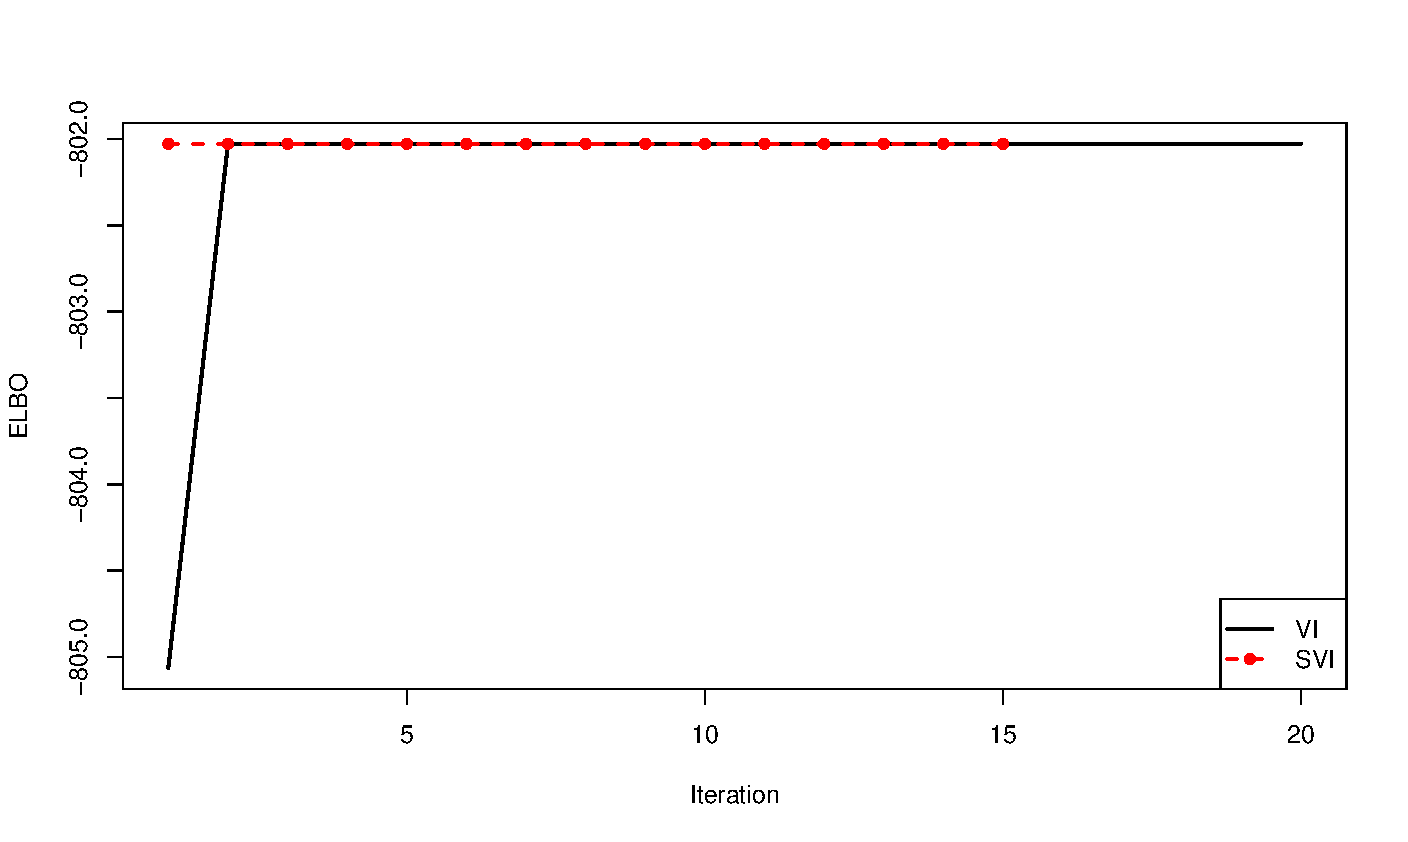
\includegraphics[scale=0.45]{Kap3/chlrm_elbo_vi_svi.pdf}
    \caption{ELBO across iterations: VI  vs.\ SVI $|S|=12$, $\epsilon=1\times10^{-7}\%,\ \chi = 0.7,\ \tau = 71.2$, simulated data.}
    \label{fig:chlrm_elbo_vi_svi}
\end{figure}

Figures~\ref{fig:chlrm_logjoint_chain}–\ref{fig:chlrm_elbo_vi_svi} assess convergence. The MCMC chain stabilizes after burn–in with a stationary mean around $-854$, evidencing satisfactory mixing. VI exhibits a smooth ascent of the ELBO, while SVI converges more erratically but to a similar bound. Together with the runtimes reported in Table~\ref{tab:fit_chlrm}, these plots highlight the trade–off: MCMC provides faithful posterior sampling but at high cost (466s), while VI and SVI achieve similar predictive performance in fractions of a second.

\begin{figure}[H]
    \centering
    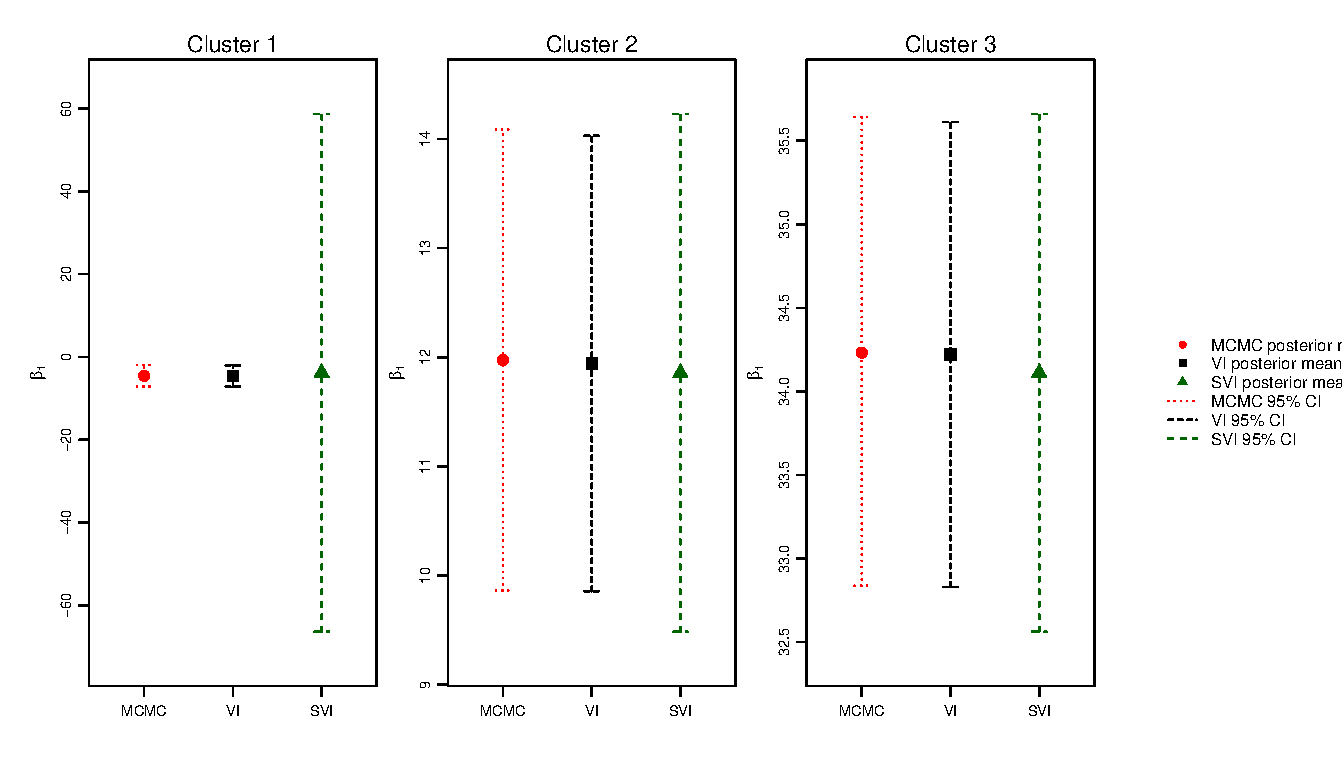
\includegraphics[scale=0.7]{Kap3/chlrm_beta1.pdf}
    \caption{Posterior summaries of $\beta_{1}$ across clusters, simulated data.}
    \label{fig:chlrm_beta1}
\end{figure}

\begin{figure}[H]
    \centering
    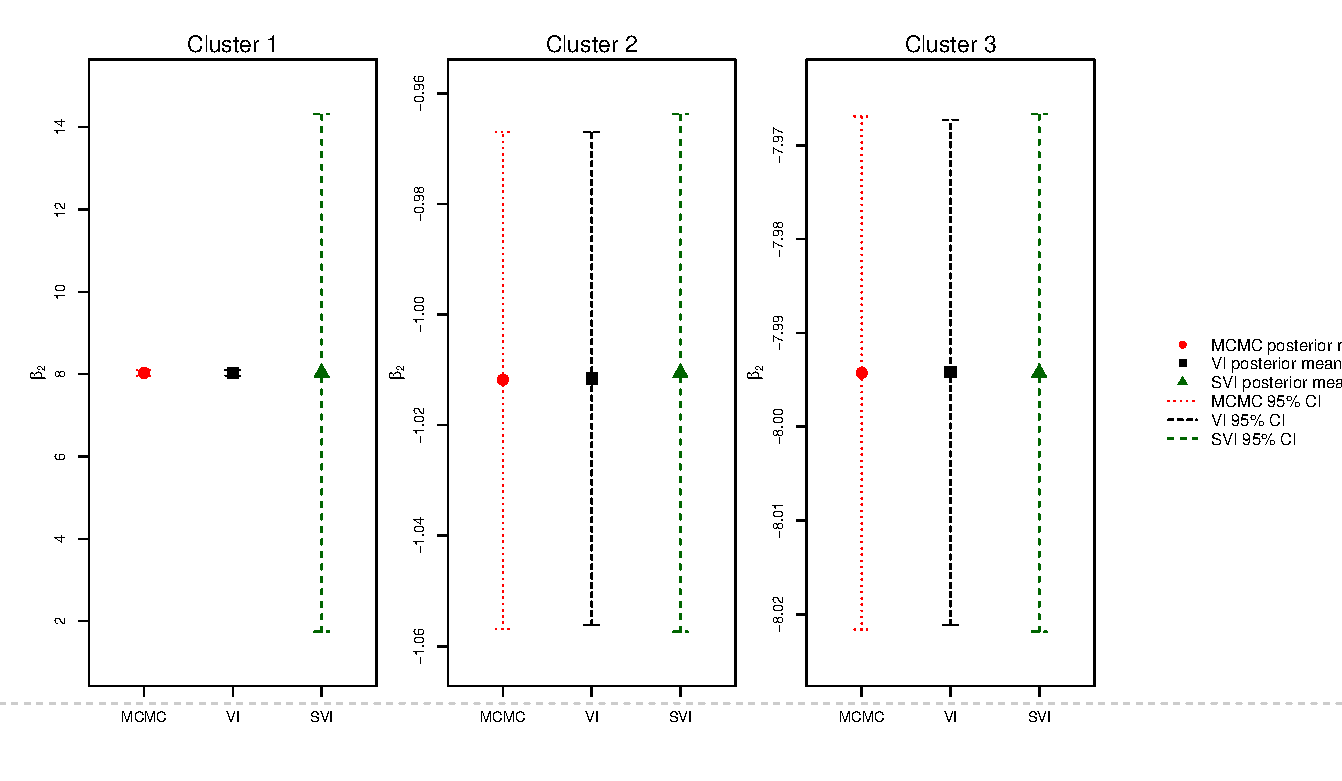
\includegraphics[scale=0.7]{Kap3/chlrm_beta2.pdf}
    \caption{Posterior summaries of $\beta_{2}$ across clusters, simulated data.}
    \label{fig:chlrm_beta2}
\end{figure}

Figures~\ref{fig:chlrm_beta1}–\ref{fig:chlrm_sigma2} confirm accurate recovery of regression slopes and error variances. Posterior means align closely with the true values, while credible intervals differ across methods: MCMC provides wider and better–calibrated intervals, whereas VI and SVI underestimate uncertainty, a known limitation of factorized approximations. This discrepancy is particularly evident for Cluster~1, where higher variability amplifies uncertainty. Nevertheless, the accuracy metrics in Table~\ref{tab:fit_chlrm} confirm the adequacy of all three methods.



\begin{table}[!h]
\centering
\caption{Goodness of fit and runtime (CHLRM, 1000 posterior samples), simulated data.}
\label{tab:fit_chlrm}
\begin{tabular}{@{} l l r r r r r @{}}
\toprule
\textbf{Method} & \textbf{Settings} & \textbf{WAIC} & \textbf{DIC} & \textbf{MSE} & \textbf{$\bm{\mathsf{R}}^2$} & \textbf{Time (s)}\\
\midrule
MCMC &
\begin{tabular}{@{}l@{}}
samples: 50000\\
burn-in: 10000\\
thin: 10
\end{tabular}
& 1453.311 & 1453.671 & 8.023 & 1 & 466.055\\
\midrule
VI &
\begin{tabular}{@{}l@{}}
iterations: 20\\
$\epsilon=1\times10^{-7}\%$
\end{tabular}
& 1453.323 & 1453.570 & 8.022 & 1 & 0.198\\
\midrule
SVI &
\begin{tabular}{@{}l@{}}
iterations: 15\\
$\epsilon=1\times10^{-7}\%$\\
$|S| = 12,\ \chi = 0.7,\ \tau = 25.8$
\end{tabular}
& 1983.810 & 2028.781 & 11.344 & 1 & 0.02\\
\bottomrule
\end{tabular}
\end{table}


\begin{figure}[H]
    \centering
    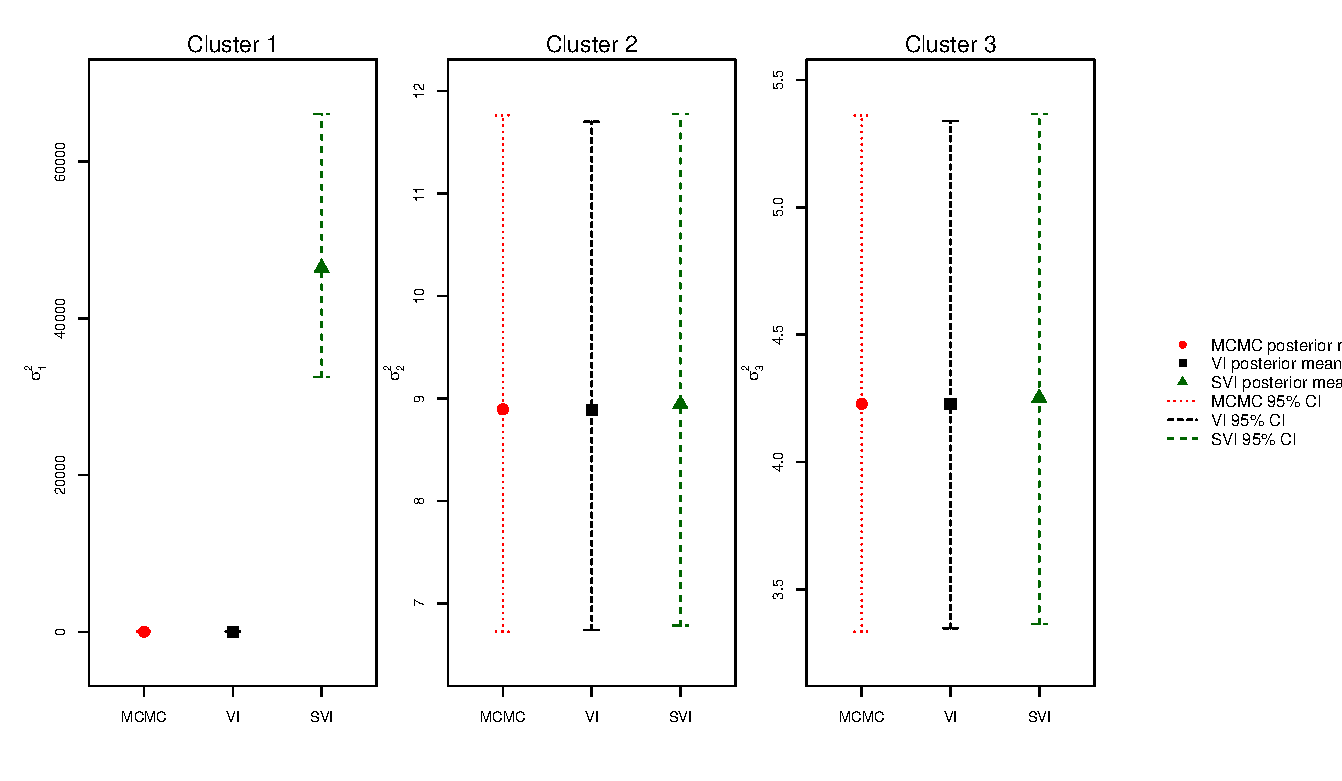
\includegraphics[scale=0.7]{Kap3/chlrm_sigma2.pdf}
    \caption{Posterior summaries of $\sigma^2_k$ across clusters , simulated data.}
    \label{fig:chlrm_sigma2}
\end{figure}



\noindent Taken together, Tables~\ref{tab:fit_chlrm} and~\ref{tab:ppp} indicate that the three inference strategies achieve nearly identical predictive accuracy. WAIC and DIC values remain virtually the same across MCMC, VI, and SVI, while MSE and $R^2$ confirm that the fitted models explain almost all of the variability in the simulated data. The posterior predictive $p$-values further reinforce this agreement: all methods yield values close to 0.5, reflecting replicated data that is statistically consistent with the observed outcomes. The combination of stable information criteria, negligible predictive error, and balanced $p_{pp}$ values demonstrates that even though VI and SVI operate under stronger approximating assumptions and achieve dramatic computational savings their predictive adequacy is not compromised relative to the gold standard provided by MCMC.

\begin{table}[!h]
\centering
\caption{\label{tab:ppp}Posterior predictive $p$-values for CHLRM (1000 replications), simulated data.}
\begin{tabular}{@{} lrrrrrr @{}}
\toprule
\textbf{Method} & \textbf{min} & \textbf{max} & \textbf{IQR} & \textbf{mean} & \textbf{median} & \textbf{sd} \\
\midrule
MCMC &  0.75 & 0.79 & 0.37 & 0.48 & 0.65 & 0.48\\
VI   & 0.73 & 0.78 & 0.35 & 0.48 & 0.65 & 0.50\\
SVI  & 0.73 & 0.79 & 0.23 & 0.50 & 0.61 & 0.53\\
\bottomrule
\end{tabular}
\end{table}


\begin{figure}[H]
    \centering
    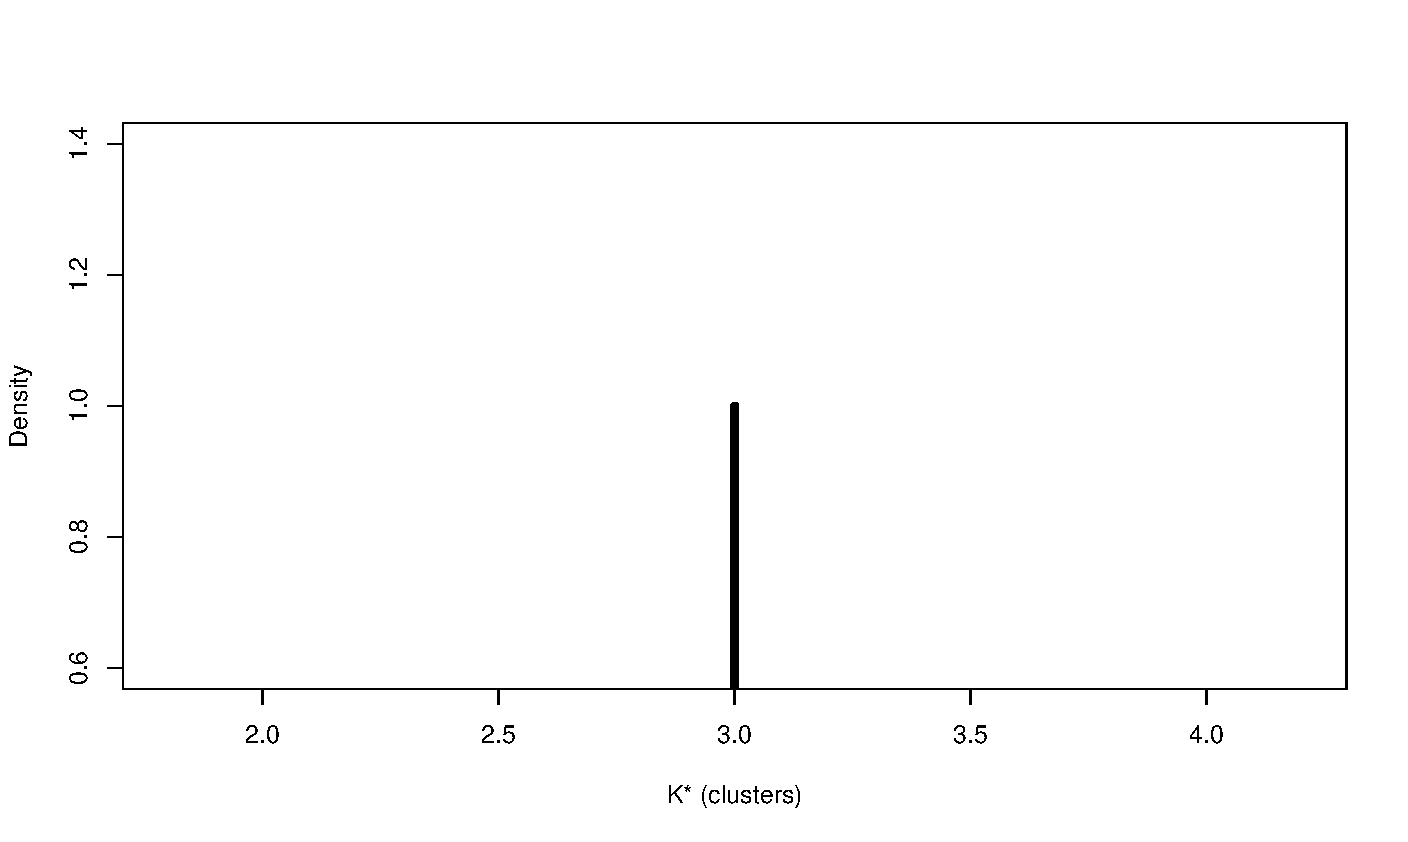
\includegraphics[scale=0.55]{Kap3/chlrm_mcmc_k.pdf}
    \caption{Posterior density of the number of non–empty clusters under MCMC with $K=14$, 50000 samples, 10000 burn-in iterations and thinned each 10 iterations, simulated data.}
    \label{fig:chlrm_mcmc_k}
\end{figure}

To get the partition size, two complementary analyses were performed. First, an MCMC run with $K=14$ estimated the posterior distribution of the number of non empty clusters (Figure~\ref{fig:chlrm_mcmc_k}), which concentrated its mass on $K=3$. Second, VI was run varying $K=1,\dots,14$ under the settings of Table~\ref{tab:fit_chlrm}; Figure~\ref{fig:chlrm_vi_k} shows that the ELBO is maximized at $K=3$, degrading for larger values. Both diagnostics consistently support the true number of clusters.

\begin{figure}[H]
    \centering
    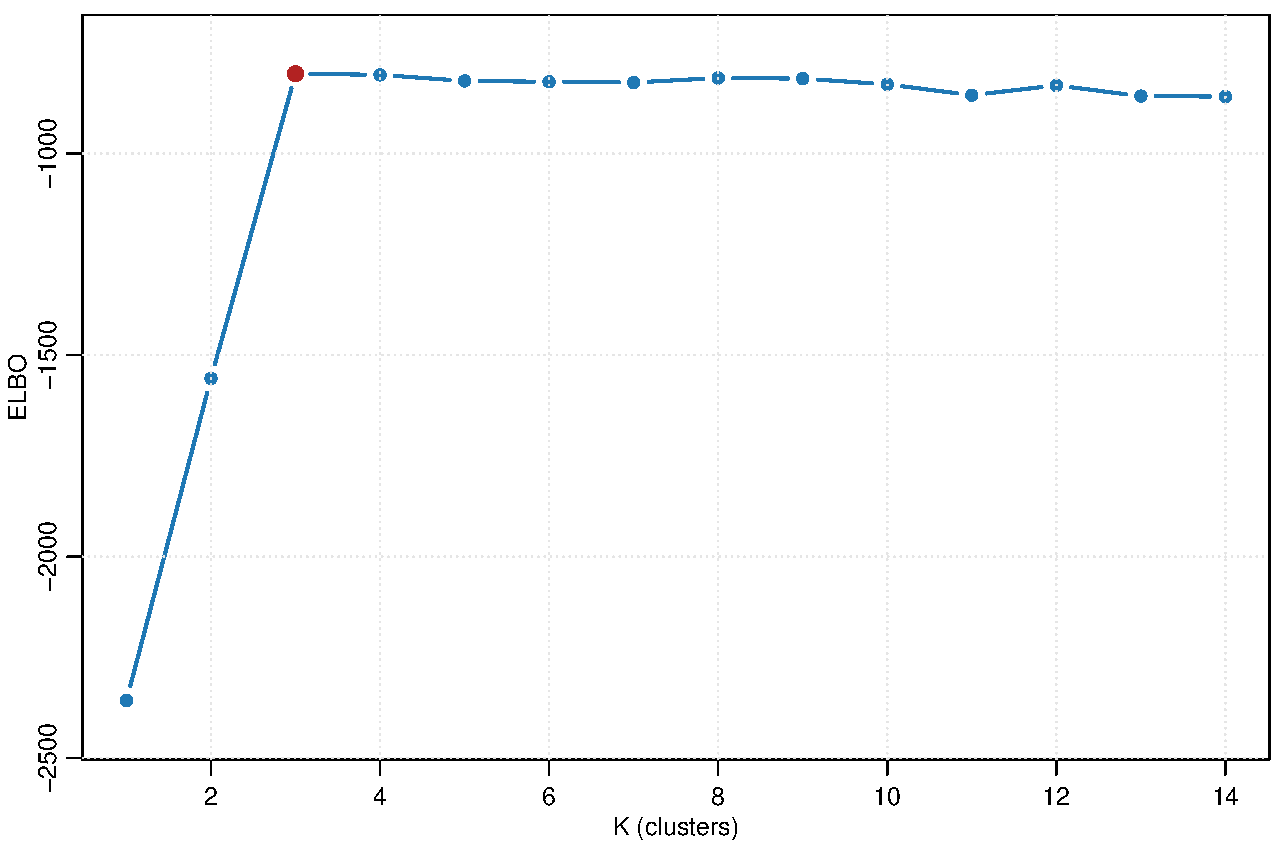
\includegraphics[scale=0.55]{Kap3/chlrm_vi_k.pdf}
    \caption{ELBO values vs.\ $K$ , simulated data.}
    \label{fig:chlrm_vi_k}
\end{figure}

The adjacency matrices in Figure~\ref{fig:chlrm_adjacency_compare} illustrate the evolution from a diffuse initialization to a clear block–diagonal structure, evidencing recovery of the true $K=3$ partition. This structural evidence complements the density fit in Figure~\ref{fig:chlrm_y_density_sim}, the parameter recovery in Figures~\ref{fig:chlrm_beta1}–\ref{fig:chlrm_sigma2}, and the metrics in Table~\ref{tab:fit_chlrm}, confirming that all methods converge to the same clustering solution, with MCMC providing the most reliable uncertainty quantification and VI/SVI offering substantial computational efficiency.

\begin{figure}[H]
    \centering
    \begin{minipage}{0.48\textwidth}
        \centering
        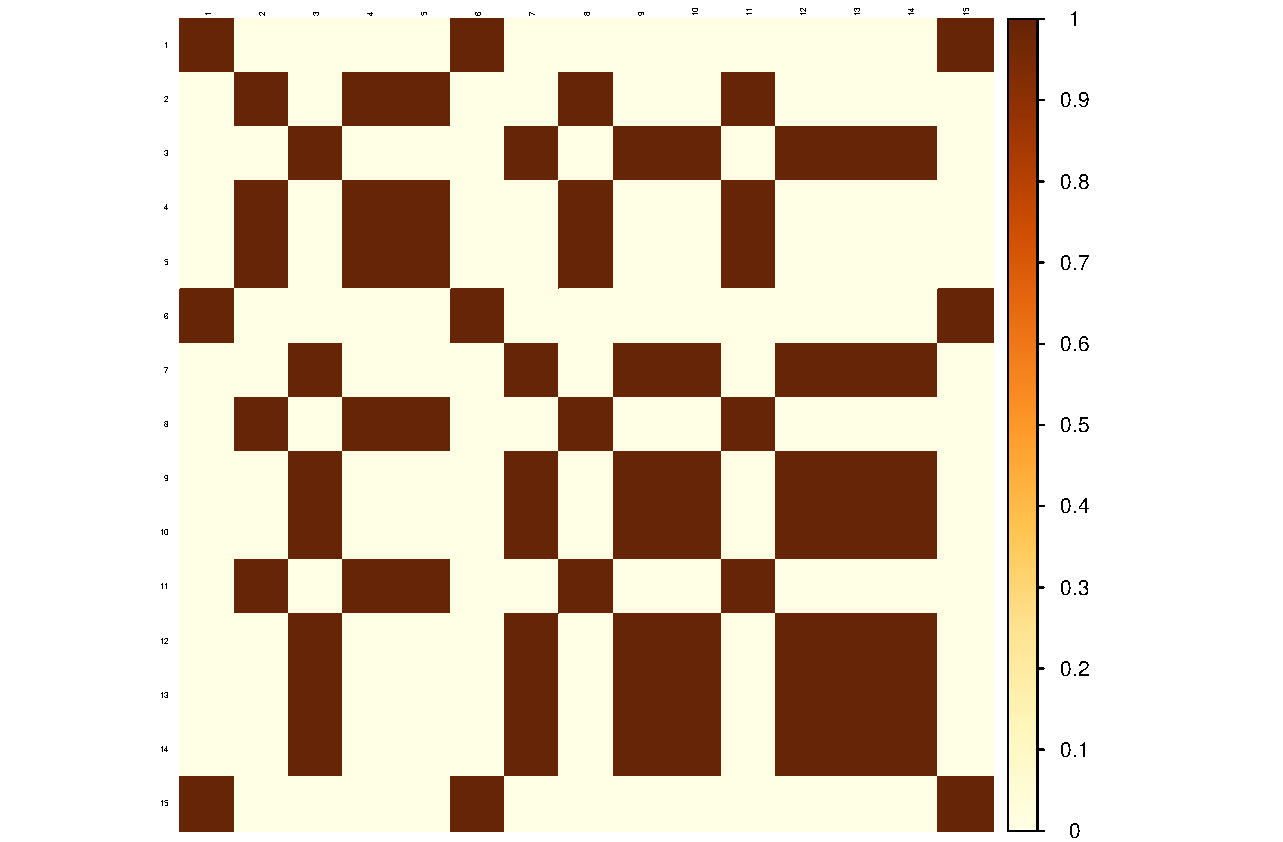
\includegraphics[width=\textwidth]{Kap3/chlrm_adjacency_init.pdf}
        \caption*{(a) Initial adjacency}
    \end{minipage}\hfill
    \begin{minipage}{0.48\textwidth}
        \centering
        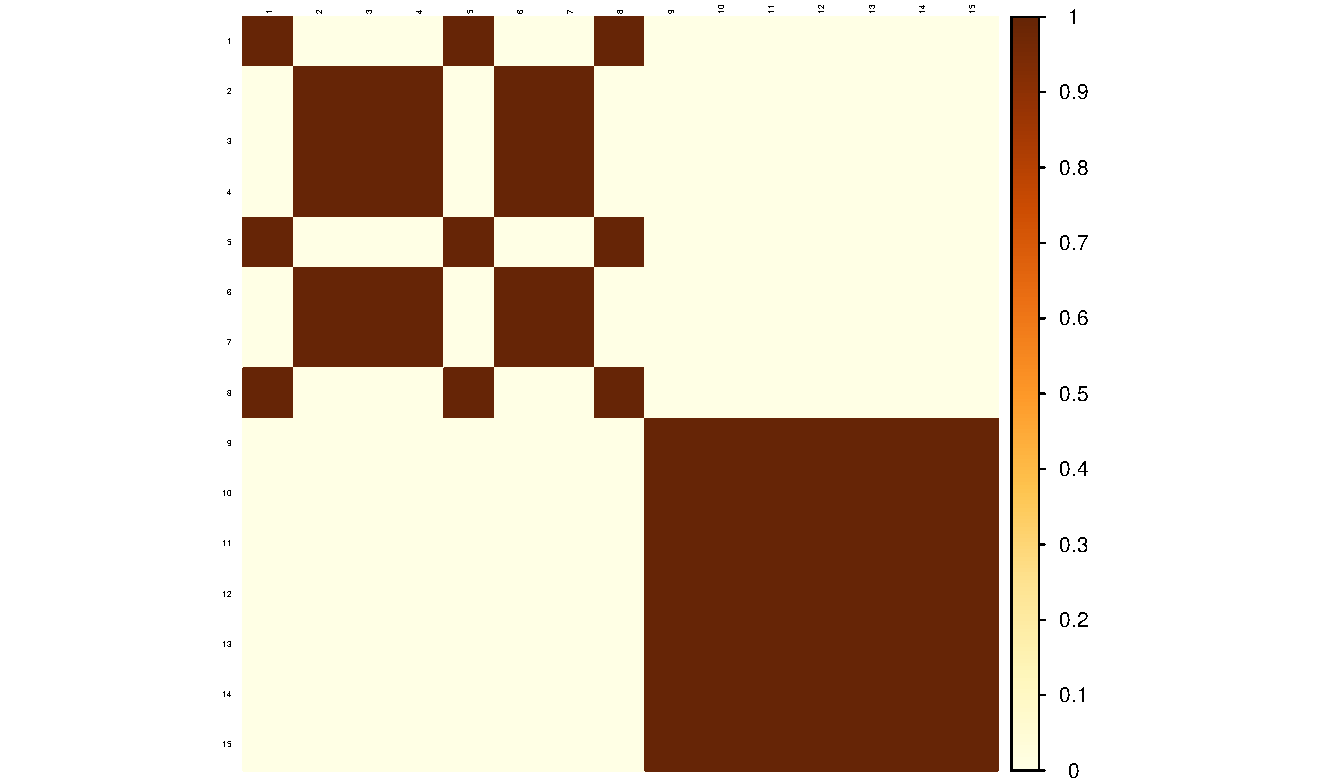
\includegraphics[width=\textwidth]{Kap3/chlrm_adjacency_final.pdf}
        \caption*{(b) Final adjacency}
    \end{minipage}
    \caption{Adjacency matrices: co–assignment probabilities between groups, simulated data.}
    \label{fig:chlrm_adjacency_compare}
\end{figure}

\subsubsection{Farms Dataset}

Returning to the farms dataset example (see Subsubsection \ref{farms}), we apply MCMC, VI, and SVI to the CHLRM with the aim of adjusting the posterior density to assess the modeling performance of these methodologies when the cluster separation is not evident. The primary goal is to obtain an optimal partition that explains farm clustering around plant sizes adjusted by soil nitrogen concentration.

\begin{figure}[H]
    \centering
    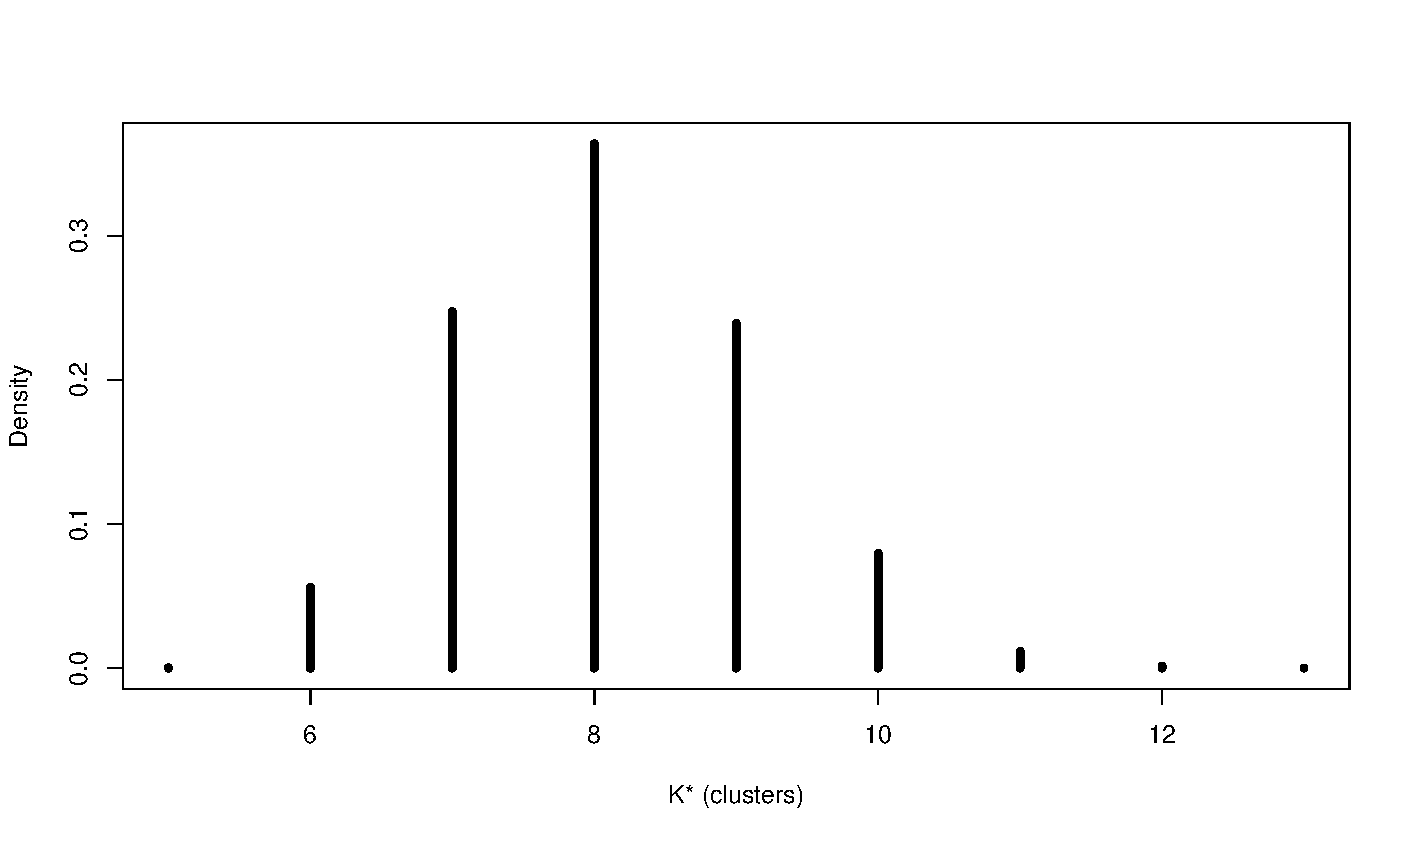
\includegraphics[scale=0.4]{Kap3/chlrm_mcmc_k_farms.pdf}
    \caption{Posterior density of the number of non–empty clusters under MCMC with $K=23$, 50000 samples, 10000 burn–in iterations, and thinning every 10 iterations, farms dataset.}
    \label{fig:chlrm_mcmc_k_farms}
\end{figure}

Figure \ref{fig:chlrm_mcmc_k_farms} shows the posterior density of the number of non–empty clusters, where the most probable values are concentrated around $K \in \{7,8,9\}$. This behavior reflects MCMC’s tendency to favor richer cluster structures, even when empirical separation is not strong. The posterior distribution remains diffuse, suggesting substantial uncertainty in the partitioning. While MCMC is asymptotically exact, its computational burden is considerable, and stabilization of the number of clusters requires long chains and careful thinning. This limitation becomes evident in runtime comparisons later in Table \ref{tab:fit_chlrm_farms}, where MCMC requires several orders of magnitude more time than VI and SVI.

\begin{figure}[H]
    \centering
    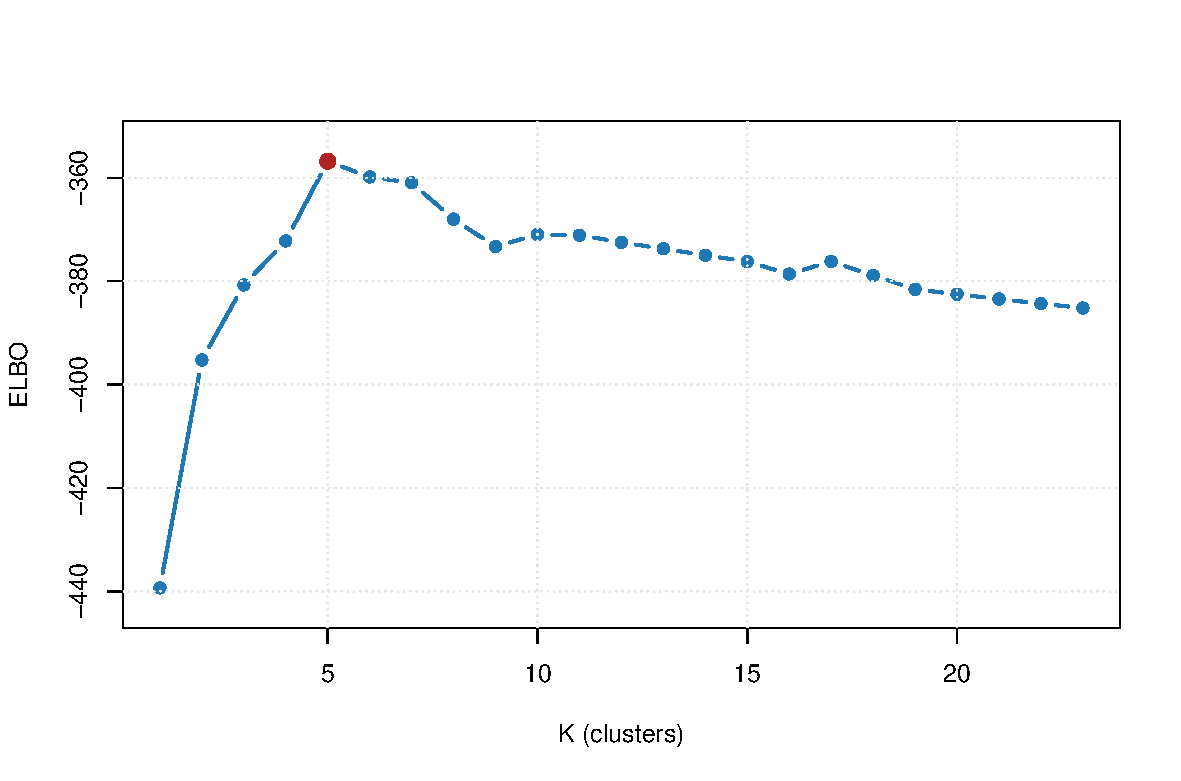
\includegraphics[scale=0.55]{Kap3/chlrm_vi_elbo_k_farms.pdf}
    \caption{ELBO values versus $K$ under SVI ($|S|=18$, $\epsilon=1\times10^{-7}\%$, $\chi = 0.7$, $\tau = 71.2$), farms dataset.}
    \label{fig:chlrm_vi_elbo_k_farms}
\end{figure}

Figure \ref{fig:chlrm_vi_elbo_k_farms} depicts the evolution of the Evidence Lower Bound (ELBO) across different $K$ values. The bound is maximized at $K=5$, favoring a more parsimonious partition compared to the higher cluster counts suggested by MCMC. The smooth trajectory of the ELBO illustrates the deterministic optimization underlying VI and SVI, which converge quickly and with reduced sensitivity to sampling noise. However, it is important to highlight that maximizing ELBO does not guarantee perfect recovery of the true number of clusters. Instead, it balances model complexity and predictive adequacy, providing computational efficiency but often underestimating posterior variance and uncertainty in cluster assignment.

\begin{figure}[H]
    \centering
    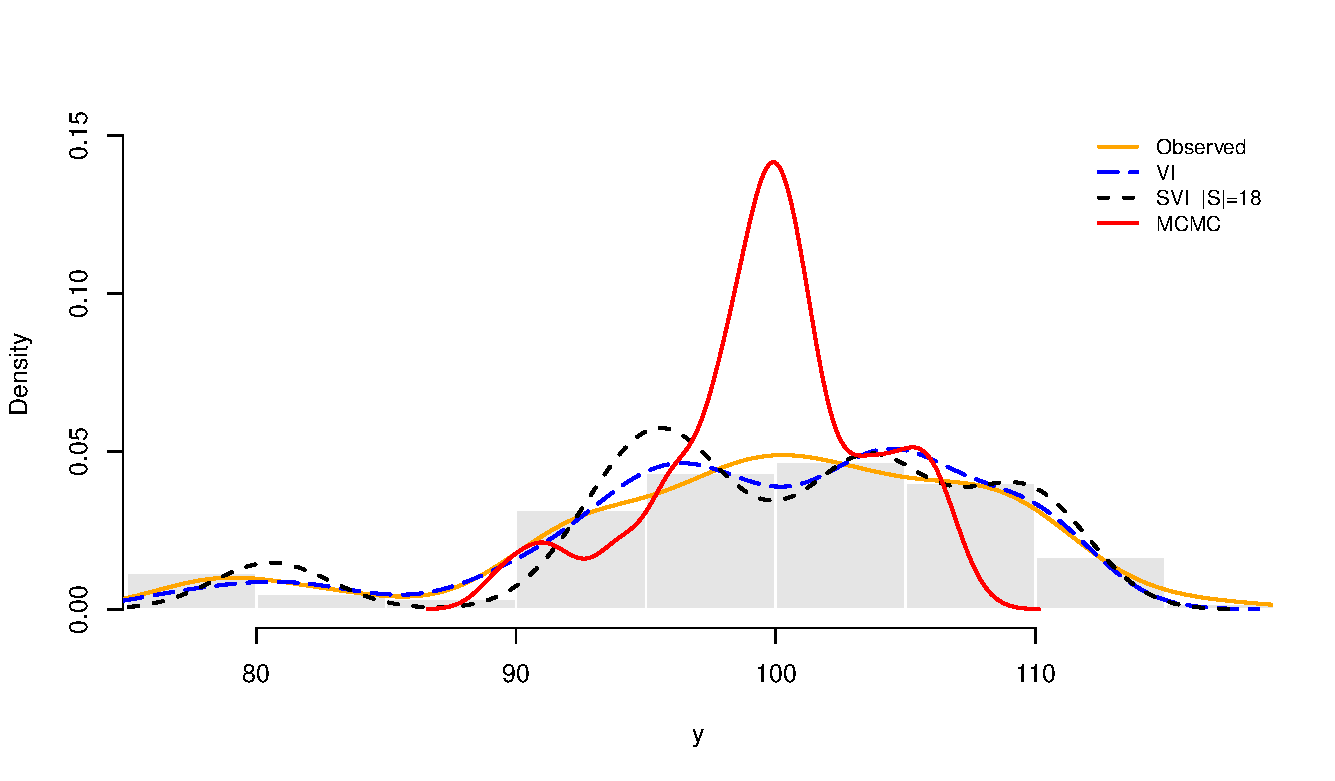
\includegraphics[scale=0.55]{Kap3/chlrm_y_density_farms.pdf}
    \caption{Observed $y$ and posterior predictive densities under MCMC, VI, and SVI with $K=5$ clusters, farms dataset.}
    \label{fig:chlrm_y_density_farms}
\end{figure}

The posterior predictive densities in Figure \ref{fig:chlrm_y_density_farms} show that all three methodologies adequately capture the global shape of the observed $y$. Nonetheless, clear differences emerge. VI and SVI produce sharper and more concentrated predictive distributions, which align more closely with the empirical data. This improved alignment is reflected in their lower MSE and higher $\mathsf{R}^2$ values reported in Table \ref{tab:fit_chlrm_farms}. By contrast, MCMC retains wider tails and higher dispersion, more faithfully representing posterior uncertainty but yielding less precise predictions. This contrast reflects the fundamental methodological trade–off: MCMC excels in posterior fidelity, whereas VI and SVI prioritize computational efficiency and predictive sharpness.

\begin{table}[!h]
\centering
\caption{\label{tab:ppp_farms}Posterior predictive $p$–values for CHLRM (1000 replications), farms dataset.}
\begin{tabular}[t]{llrrrrrr}
\toprule
\textbf{Method} & \textbf{min} & \textbf{max} & \textbf{IQR} & \textbf{mean} & \textbf{median} & \textbf{sd} \\
\midrule
MCMC & 0.34 & 0.33 & 0.23 & 0.50 & 0.46 & 0.56\\
VI & 0.12 & 0.31 & 0.33 & 0.50 & 0.52 & 0.56\\
SVI & 0.13 & 0.19 & 0.30 & 0.56 & 0.58 & 0.64\\
\bottomrule
\end{tabular}
\end{table}

Posterior predictive $p$–values in Table \ref{tab:ppp_farms} reinforce the adequacy of all three methods, as mean and median values are close to 0.5, indicating good calibration of predictive distributions. SVI exhibits slightly higher central values, suggesting an optimistic fit to the observed statistics, consistent with \cite{HOFF}. MCMC produces more balanced values across discrepancy measures, though with greater variability, whereas VI delivers stable but slightly conservative predictive outcomes.

\newpage

\begin{table}[!h]
\centering
\caption{Goodness of fit and runtime (CHLRM, 1000 posterior samples), farms dataset.}
\label{tab:fit_chlrm_farms}
\begin{tabular}{@{} l l r r r r r @{}}
\toprule
\textbf{Method} & \textbf{Settings} & \textbf{WAIC} & \textbf{DIC} & \textbf{MSE} & \textbf{$\bm{\mathsf{R}}^2$} & \textbf{Time (s)}\\
\midrule
MCMC &
\begin{tabular}{@{}l@{}}
samples: 120000\\
burn–in: 30000\\
thin: 20
\end{tabular}
& 570.278 & 583.640 & 30.711 & 0.579 & 3039.362\\
\midrule
VI &
\begin{tabular}{@{}l@{}}
iterations: 11\\
$\epsilon=1\times10^{-7}\%$
\end{tabular}
& 574.070 & 579.002 & 6.330 & 0.913 & 0.020\\
\midrule
SVI &
\begin{tabular}{@{}l@{}}
iterations: 2496\\
$\epsilon=1\times10^{-1}\%$\\
$|S| = 18,\ \chi = 0.7,\ \tau = 71.2$
\end{tabular}
& 615.305 & 624.503 & 5.948 & 0.918 & 3.848\\
\bottomrule
\end{tabular}
\end{table}

Table \ref{tab:fit_chlrm_farms} summarizes the explicit trade–offs. MCMC achieves the lowest WAIC and DIC, underscoring its stronger posterior adherence, but incurs prohibitive runtime (over 3000 seconds). VI and SVI, on the other hand, drastically reduce runtime to fractions of a second or a few seconds, while achieving superior $\mathsf{R}^2$ and lower MSE. Their information criteria values, however, are slightly inflated, reflecting the bias introduced by variational approximations. These results show that the variational algorithms, while highly scalable, may sacrifice posterior fidelity when cluster separation is weak.

\begin{figure}[H]
    \centering
    \begin{minipage}{0.5\textwidth}
        \centering
        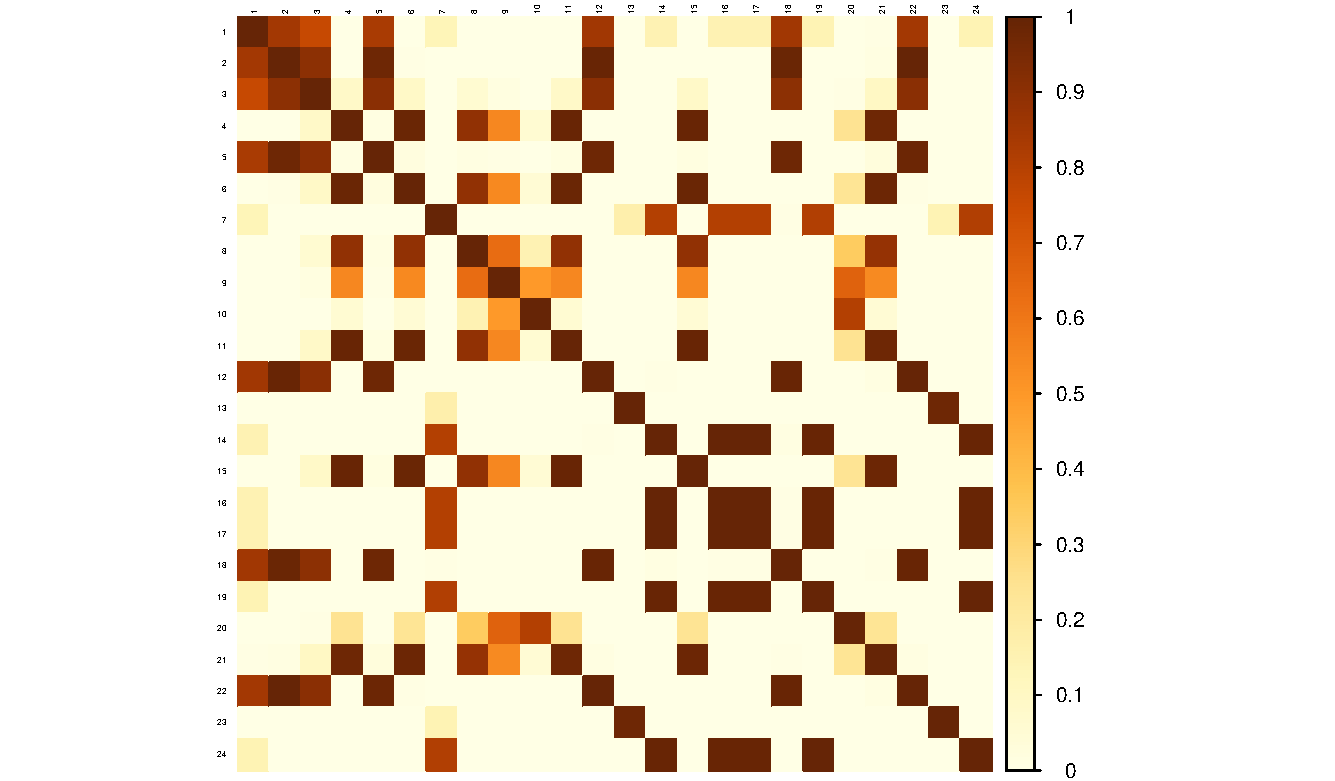
\includegraphics[width=\textwidth]{Kap3/chlrm_mcmc_A_init.pdf}
        \caption*{(a) Initial adjacency}
    \end{minipage}\hfill
    \begin{minipage}{0.5\textwidth}
        \centering
        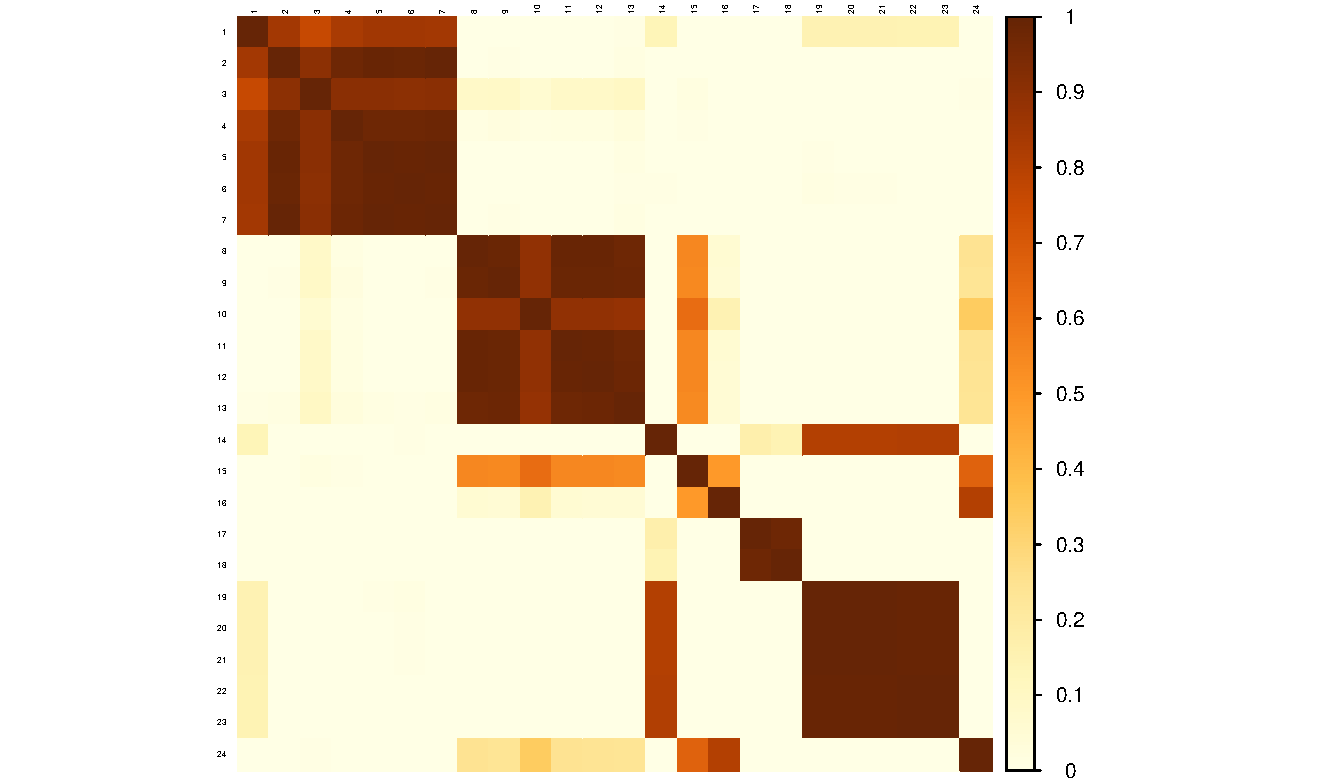
\includegraphics[width=\textwidth]{Kap3/chlrm_mcmc_A_fin.pdf}
        \caption*{(b) Final adjacency}
    \end{minipage}
    \caption{Adjacency matrices: co–assignment probabilities between groups under MCMC, farms dataset.}
    \label{fig:chlrm_mcmc_A_compare}
\end{figure}

\begin{figure}[H]
    \centering
    \begin{minipage}{0.5\textwidth}
        \centering
        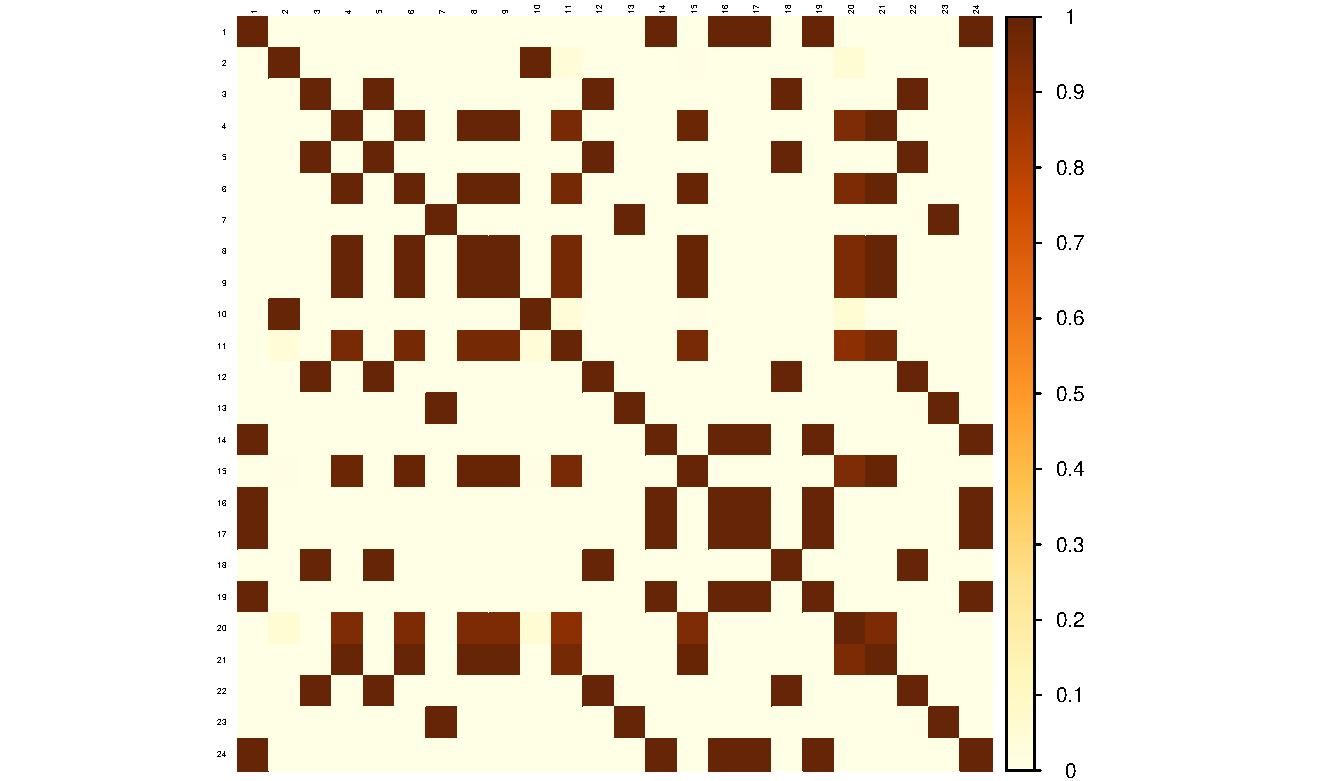
\includegraphics[width=\textwidth]{Kap3/chlrm_vi_A_init.pdf}
        \caption*{(a) Initial adjacency}
    \end{minipage}\hfill
    \begin{minipage}{0.5\textwidth}
        \centering
        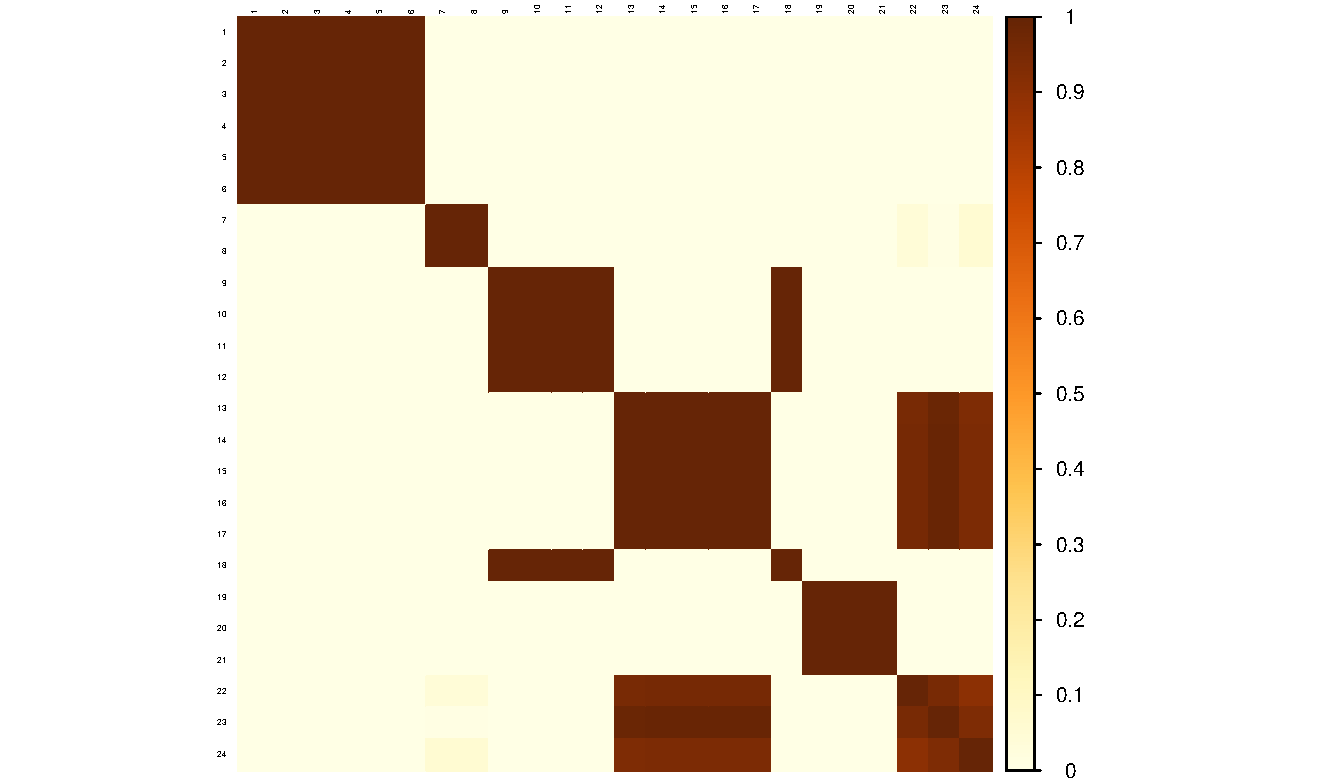
\includegraphics[width=\textwidth]{Kap3/chlrm_vi_A_fin.pdf}
        \caption*{(b) Final adjacency}
    \end{minipage}
    \caption{Adjacency matrices: co–assignment probabilities between groups under VI, farms dataset.}
    \label{fig:chlrm_vi_A_compare}
\end{figure}

\begin{figure}[H]
    \centering
    \begin{minipage}{0.5\textwidth}
        \centering
        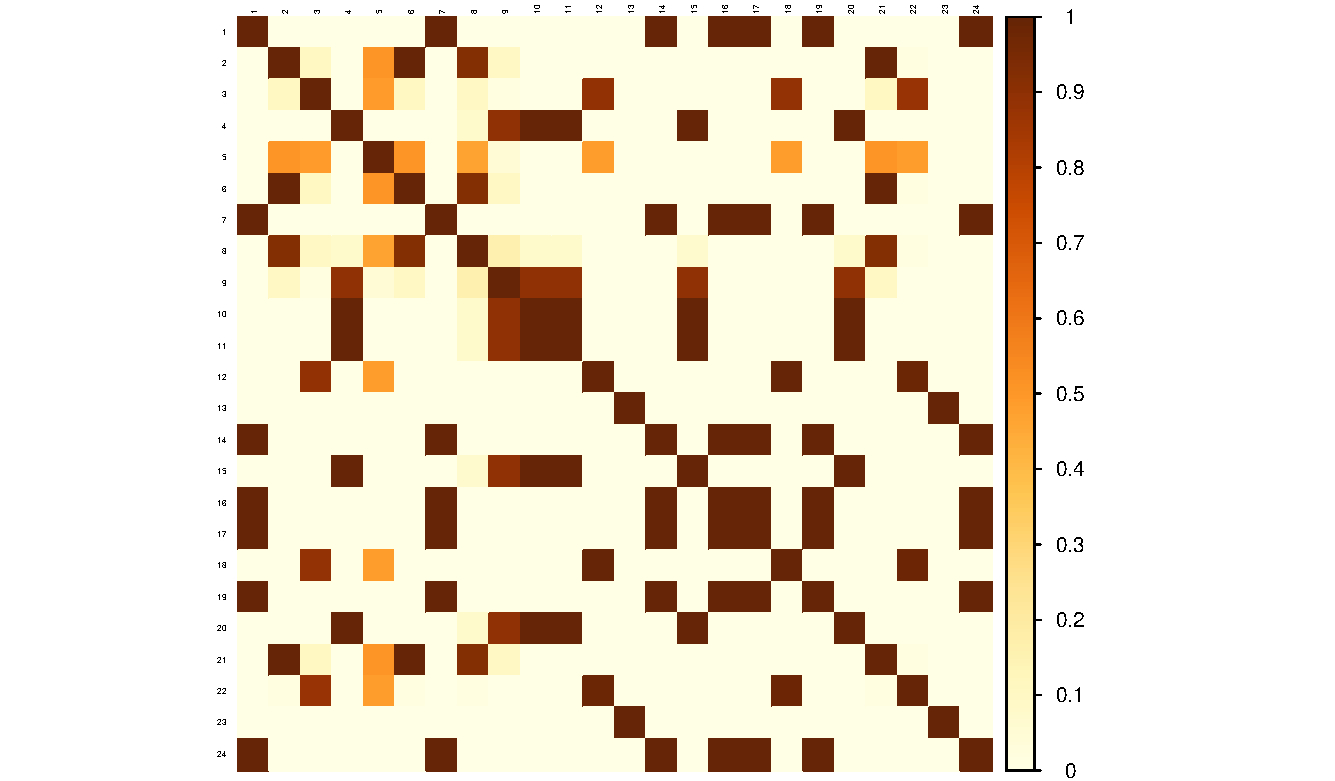
\includegraphics[width=\textwidth]{Kap3/chlrm_svi_A_init.pdf}
        \caption*{(a) Initial adjacency}
    \end{minipage}\hfill
    \begin{minipage}{0.5\textwidth}
        \centering
        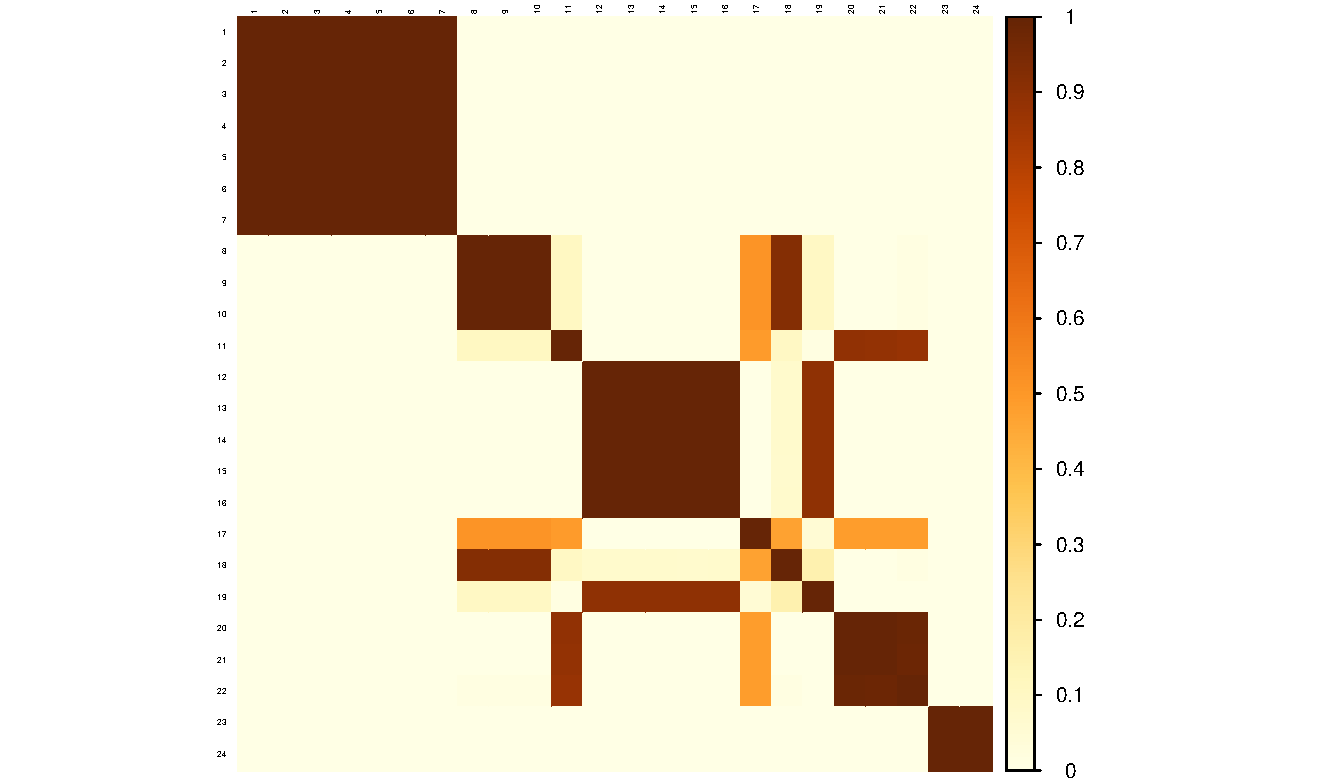
\includegraphics[width=\textwidth]{Kap3/chlrm_svi_A_fin.pdf}
        \caption*{(b) Final adjacency}
    \end{minipage}
    \caption{Adjacency matrices: co–assignment probabilities between groups under SVI, farms dataset.}
    \label{fig:chlrm_svi_A_compare}
\end{figure}

The adjacency matrices in Figures \ref{fig:chlrm_mcmc_A_compare}, \ref{fig:chlrm_vi_A_compare}, and \ref{fig:chlrm_svi_A_compare} provide a qualitative assessment of co–assignment probabilities. MCMC gradually transitions from diffuse initial states to sharper block structures, reflecting its ability to capture fine–grained posterior co–clustering. VI converges more quickly to rigid partitions, but with reduced representation of uncertainty. SVI strikes a balance: its final adjacency matrices show clear cluster delineation achieved in shorter time, though with additional stochastic variability introduced by mini–batch updates. 

\vspace{0.5cm}

In summary, the farms dataset highlights the core trade–offs of MCMC, VI, and SVI in clustered hierarchical regression. MCMC provides the most faithful posterior inference, as reflected in lower information criteria and richer adjacency structures, but at prohibitive computational cost. VI offers speed and stable convergence, producing sharp predictive fits at the expense of underestimating posterior variance. SVI emerges as a middle ground: it scales efficiently, delivers predictive accuracy close to VI, and produces adjacency structures that capture cluster patterns more robustly than VI alone, but it inherits stochastic noise and some bias in posterior uncertainty. Thus, while MCMC remains the gold standard in terms of posterior fidelity, VI and SVI provide practical alternatives when runtime and scalability are critical, particularly in datasets with weak cluster separation.

\chapter{Discussion \& Conclusions}

This thesis has examined Bayesian inference for regression models of increasing complexity, ranging from the Linear Regression Model (LRM), through the Hierarchical Linear Regression Model (HLRM), to the Clustered Hierarchical Linear Regression Model (CHLRM). Across these settings, we contrasted the gold standard of Markov Chain Monte Carlo (MCMC) with two deterministic alternatives: Variational Inference (VI) and Stochastic Variational Inference (SVI). Our central objective was to assess the trade-off between computational scalability and statistical fidelity, clarifying when optimization-based approximations can stand in for simulation-based inference and when their limitations become decisive.

\vspace{0.3cm}

The analysis of the LRM demonstrated that, under simple model structures, VI and SVI yield posterior summaries and predictive distributions that are nearly indistinguishable from those obtained by MCMC. Performance metrics such as WAIC, DIC, $R^2$, and MSE all indicated minimal loss in statistical accuracy, while computation times were reduced by an order of magnitude. This reinforces the growing consensus in the literature \cite{Ormerod2010-bc, Blei2016VariationalIA, zhang2018advancesvariationalinference} that in low-dimensional or conjugate models, variational methods provide a reliable and efficient surrogate for MCMC.

\vspace{0.3cm}

The hierarchical case highlighted the limitations of variational approximations. As shown in Table~\ref{tab:goodness}, MCMC clearly outperformed VI and SVI in information criteria, achieving $\mathsf{WAIC}=545.1$ and $\mathsf{DIC}=545.8$, while VI and SVI yielded substantially higher values ($\mathsf{WAIC}\approx 1316$--$1327$, $\mathsf{DIC}\approx 1333$--$1338$). This gap underscores MCMC’s ability to preserve group-level heterogeneity and parameter dependencies. By contrast, VI and SVI systematically underestimated variance components, especially for the group intercepts $\beta_{j,1}$ and $\sigma_j^2$. This pattern, illustrated in figure \ref{fig:hlrm_y_density_farms}, reflects the mean–field assumption: by factorizing the posterior into independent marginals, posterior correlations are lost and credible intervals are distorted. Nonetheless, both VI and SVI correctly recovered the main regression effects and displayed the expected shrinkage of group-level estimates. Their runtime advantage remained considerable, converging in seconds compared to hundreds of seconds for MCMC.

\vspace{0.3cm}

This phenomenon has been extensively discussed in the literature \cite{Blei2006-kd, Wainwright2007-ul, wang22g}, and arises from the mean–field assumption at the core of standard variational methods: by factorizing the posterior into independent components, these algorithms reduce dependencies and consequently shrink posterior variances. Our results confirmed this theoretical expectation, with Figure and ~\ref{fig:hlrm_sigma2j_farms} clearly 

\vspace{0.3cm}

An important perspective is offered in \cite{Blei2016VariationalIA}, who emphasize that variational inference, while computationally appealing, systematically underestimates posterior variances due to the asymmetric nature of the Kullback–Leibler divergence employed in its optimization objective. This theoretical insight directly resonates with our empirical findings in the hierarchical and clustered settings: both VI and SVI tended to deliver credible intervals narrower than those produced by MCMC, particularly for variance components. The underestimation is not an artifact of our implementation but a structural limitation of mean–field variational methods, which penalize allocating mass to regions of low posterior density more strongly than they reward covering regions of high posterior support. In practice, this results in posterior approximations that reproduce central tendencies effectively but attenuate dispersion. Our results confirm this behavior across increasingly complex models. 

\vspace{0.3cm}

The clustered extension posed a more balanced scenario. As reported in Table~\ref{tab:fit_chlrm_farms}, MCMC achieved $\mathsf{WAIC}=570.3$ and $\mathsf{DIC}=583.6$, while VI and SVI produced values of similar order ($\mathsf{WAIC}=574.1$ and $615.3$, $\mathsf{DIC}=579.0$ and $624.5$, respectively). Unlike the hierarchical case, the performance gap was narrower: although MCMC retained the best fit, VI and SVI approximated it reasonably well. More importantly, all three methods recovered the same clustering partition, as shown in the adjacency matrices of Figure~\ref{fig:chlrm_mcmc_A_compare}. This suggests that, despite limitations in variance estimation, this suggests that although VI and SVI distort posterior uncertainty, they still succeed in identifying global structures such as clusters, corroborating findings by \cite{Blei2006-kd, HOFFMAN,beal2003variational}. For applied contexts where clustering accuracy outweighs exact posterior calibration, this robustness is of practical significance.

\vspace{0.3cm}

A striking empirical result is the similarity between VI and SVI across all models. Both methods optimize the same Evidence Lower Bound (ELBO) under the same mean–field family; the only difference is that SVI employs stochastic natural gradients and mini-batching \cite{HOFFMAN, VAE}. In the moderate sample sizes of our experiments, gradient noise was small, and both approaches converged to virtually identical solutions. This explains why SVI did not show a marked advantage over VI in our study, though it remains essential for large-scale or streaming data.

\vspace{0.3cm}

Taken together, these results illustrate the core trade-off of Bayesian computation. MCMC remains unparalleled in preserving dependencies and delivering calibrated posterior intervals, but incurs heavy computational costs. VI and SVI, in contrast, deliver drastic computational gains by recasting inference as optimization over restricted families, at the cost of underestimating posterior uncertainty and producing unreliable information criteria. This duality echoes the theoretical accounts of \cite{Wainwright2007-ul, Blei2016VariationalIA, zhang2018advancesvariationalinference}, which highlight both the appeal and the risks of variational methods. Our empirical findings align with this literature, but add clarity by showing how these trade-offs manifest concretely in hierarchical and clustered regression contexts.

\vspace{0.3cm}

From a methodological standpoint, the strengths and weaknesses of each algorithm can now be summarized. MCMC is statistically reliable and broadly applicable, but slow. VI and SVI are fast and scalable, but variance underestimation and distorted posteriors are intrinsic limitations of the mean–field framework. The pedagogical contribution of this work lies in making these contrasts explicit through derivations, simulations, and reproducible implementations. Computationally, the development of VI and SVI algorithms required careful derivation of natural gradients and coordinate updates, with practical challenges in initialization and convergence monitoring. These hurdles underscore the importance of strong mathematical foundations in implementing scalable Bayesian inference.

\vspace{0.3cm}

Looking forward, the limitations observed here point to clear avenues for future research. Richer variational families, such as structured VI \cite{wang22g} or flow-based approximations, offer the promise of mitigating variance underestimation while retaining scalability. Hybrid methods, where VI provides rapid initialization and MCMC refines the posterior, are another promising direction \cite{Blei2016VariationalIA, zhang2018advancesvariationalinference}. Finally, applying these algorithms to large-scale educational or biomedical data would test their practical limits, validating whether the patterns observed in simulations extend to complex real-world settings.

\vspace{0.3cm}

In conclusion, this thesis has clarified the comparative performance of MCMC, VI, and SVI for hierarchical and clustered regression models, highlighting both the contexts where variational methods are reliable and the domains where their limitations are critical. By bridging theoretical insights with computational practice and empirical evaluation, the work contributes not only to the methodological literature but also to the accessibility of advanced Bayesian computation for applied researchers. The open-source implementation ensures reproducibility and fosters further development, supporting the broader dissemination of Bayesian methods in the statistical community.


%\include{Kap5/Kap5}
%\include{Kap6/Kap6}
\begin{appendix}
\chapter{Notation}
\label{Appendix_A}

\section{ Natural Exponential Family}

\cite{ML_MURPHY} A pdf or pmf $p(\bm{x} \mid \bm{\theta})$,  belongs to the \emph{natural exponential family} it is $\bm{x}\sim \mathsf{NEF}(\bm{\eta})$, if its density (or mass) function can be written as:

\begin{equation}
\label{NEF}
p(\bm{x} \mid \bm{\eta}) = h(\bm{x})\, \exp\left\{ \bm{\eta}^\top \bm{t}(\bm{x}) - a(\bm{\eta}) \right\} 
\end{equation}

where:

\begin{itemize}
\item $\bm{\eta} = g(\bm{\theta})  \ \leftrightarrow \ \bm{\theta} = g^{-1}(\bm{\eta})$, with $g(\cdot)$ is a function that maps the parameters $\bm{\theta}$ to the natural parameters $\bm{\eta}$.
\item $h(\bm{x})$ is the base measure (e.g. Lebesgue measure).
\item $\bm{t}(\bm{x})$ is the sufficient statistic.
\item $a(\bm{\eta})$ is the log-partition function (log normalizer), such that:

$$
\int h(\bm{x}) \exp\left\{ \bm{\eta}^\top \bm{t}(\bm{x}) - a(\bm{\eta}) \right\} d\bm{x} = 1
$$

That is:

\begin{equation}
a(\bm{\eta}) = \log\left( \int h(\bm{x}) \exp\left\{ \bm{\eta}^\top \bm{t}(\bm{x}) \right\} d\bm{x} \right)
\end{equation}

And satisfies:

\begin{itemize}
\item[a)] $\nabla_{\bm{\eta}} a(\bm{\eta}) = \mathsf{E}_{\bm{\eta}}\left[\bm{t}(\bm{x})\right]$
\item[b)] $\nabla_{\bm{\eta}}^2 a(\bm{\eta}) = \mathsf{Var}_{\bm{\eta}}\left[\bm{t}(\bm{x})\right]$
\end{itemize}
\end{itemize}

\section{ Distributions}

\begin{itemize}

\item \textbf{Multivariate normal:}

A $d \times 1$ random vector $\bm{X} = (X_1, \dots, X_d)^\top$ has a multivariate Normal distribution with parameters $\bm{\mu}$ and $\bm{\Sigma}$, denoted by $\bm{X} \mid \bm{\mu}, \bm{\Sigma} \sim \mathsf{N}_d(\bm{\mu}, \bm{\Sigma})$, if its density function is:

$$
p(\bm{x} \mid \bm{\mu}, \bm{\Sigma}) = (2\pi)^{-d/2} |\bm{\Sigma}|^{-1/2} \exp\left\{ -\frac{1}{2} (\bm{x} - \bm{\mu})^\top \bm{\Sigma}^{-1} (\bm{x} - \bm{\mu}) \right\}
$$

\begin{itemize}
\item \textit{Sufficient statistics:} $\bm{t}(\bm{x}) = \left(\bm{x},\ \bm{x}^\top\bm{x}\right)^\top$
\item \textit{Natural parameter:} $
\bm{\eta} = \left( \bm{\Sigma}^{-1} \bm{\mu},\ -\frac{1}{2} \bm{\Sigma}^{-1} \right)^\top
$
\item \textit{Inverse mapping:} Given $\bm{\eta} = \left(\bm{\eta}_1,\ \bm{\eta}_2\right)^\top$, 
$$
\bm{\Sigma} = -\tfrac{1}{2}\bm{\eta}_2^{-1}, \qquad \bm{\mu} = -\tfrac{1}{2}\bm{\eta}_2^{-1}\bm{\eta}_1.
$$
\item \textit{Key Expectations:} 
\begin{itemize}
\item $\mathsf{E}[\bm{X}] = \bm{\mu}$
\item  $\mathsf{E}[\bm{X}^\top\bm{X}] = \bm{\Sigma} + \bm{\mu}^\top\bm{\mu}$
\item $\mathsf{E}[\log p(\bm{X} \mid \bm{\mu}, \bm{\Sigma})]=-\frac{d}{2}\log(2\pi e)-\frac{1}{2}\log|\bm{\Sigma}|$
\end{itemize}
\end{itemize}

\item \textbf{Gamma:}

A random variable $X$ has a Gamma distribution with parameters $\alpha, \beta > 0$, denoted by $X \mid \alpha, \beta \sim \mathsf{G}(\alpha, \beta)$, if its density function is:

$$
p(x \mid \alpha, \beta) = \frac{\beta^\alpha}{\Gamma(\alpha)} x^{\alpha - 1} \exp\{-\beta x\} \footnote{The the gamma function $\Gamma(\cdot)$:

$$
\Gamma(z) = \int_0^\infty t^{z-1}e^{-t}dt
$$
}, \quad x > 0
$$

\begin{itemize}
\item \textit{Sufficient statistics:} $\bm{t}(x) = \left(\log x,\ x\right)^\top$
\item \textit{Natural parameter:} $\bm{\eta} = (\alpha - 1,\ -\beta)^\top$
\item \textit{Inverse mapping :} Given $\bm{\eta} = (\eta_1,\ \eta_2)^\top$, 
$$
\alpha = \eta_1 + 1, \qquad \beta = -\eta_2.
$$
\item \textit{Key Expectations:}
\begin{itemize}
\item $\mathsf{E}[X] = \dfrac{\alpha}{\beta}$
\item $\mathsf{E}[\log X] = \psi(\alpha) - \log \beta$ \footnote{The digamma function $\psi(\cdot)$ is defined as the logarithmic derivative of the Gamma function:
$$
\psi(z) = \frac{d}{dz} \log \Gamma(z) = \frac{\Gamma'(z)}{\Gamma(z)}
$$}
\item $\mathsf{E}[\log p(X \mid \alpha, \beta) ]=\log\beta-\log\Gamma(\alpha)+(\alpha-1)\psi(\alpha)-\alpha$
\end{itemize}
\end{itemize}

\item \textbf{Inverse Gamma:}

A random variable $X$ has an Inverse Gamma distribution with parameters $\alpha, \beta > 0$, denoted by $X \mid \alpha, \beta \sim \mathsf{IG}(\alpha, \beta)$, if its density function is:

$$
p(x \mid \alpha, \beta) = \frac{\beta^\alpha}{\Gamma(\alpha)} x^{-(\alpha + 1)} \exp\left\{ -\frac{\beta}{x} \right\}, \quad x > 0
$$

\begin{itemize}
\item \textit{Sufficient statistics:} $\bm{t}(x) = \left(\log x,\ \dfrac{1}{x}\right)^\top$
\item \textit{Natural Parameter:} $\bm{\eta} = (-\alpha - 1,\ -\beta)^\top$
\item \textit{Inverse mapping:} Given $\bm{\eta} = (\eta_1,\ \eta_2)^\top$, 
$$
\alpha = -\eta_1 - 1, \qquad \beta = -\eta_2.
$$
\item \textit{Key Expectations:} 
\begin{itemize}
\item $\mathsf{E}[X] = \dfrac{\beta}{\alpha-1}$, for $\alpha>1$
\item $\mathsf{E}[\frac{1}{X}] = \dfrac{\alpha}{\beta}$
\item $\mathsf{E}[\log X] = \log \beta - \psi(\alpha)$
\item $\mathsf{E}[\log p(X \mid \alpha, \beta)] =-\log\beta-\log\Gamma(\alpha)+(\alpha+1)\psi(\alpha)-\alpha$
\end{itemize}
\end{itemize}

\newpage

\item \textbf{Inverse Wishart:}

A $d \times d$ random matrix $\bm{W}$ has an Inverse Wishart distribution with parameters $\nu$ and $\bm{S}^{-1}$, denoted by $\bm{W}\mid\nu, \bm{S}^{-1} \sim \mathsf{IW}(\nu, \bm{S}^{-1})$, if its density function is:

$$
p(\bm{W}\mid\nu, \bm{S}^{-1}) =\dfrac{|\bm{S}|^{\frac{\nu}{2}}}{2^{\frac{d\nu}{2}}\Gamma_d{(\frac{\nu}{2})}}|\bm{W}|^{-(\nu + d + 1)/2} \exp\left\{ -\frac{1}{2} \operatorname{tr}(\bm{S} \bm{W}^{-1}) \right\}\footnote{The multivariate gamma function $\Gamma_d(\cdot)$: $$\Gamma_d(\alpha) = \pi^{d(d-1)/4} \prod_{j=1}^{d} \Gamma(\alpha - (j-1)/2)$$} , \quad \nu > 0, \quad \bm{S} > 0
$$

\begin{itemize}
\item \textit{Sufficient statistics:}  $\bm{t}(\bm{W}) = \left(\bm{W}^{-1},\ \log|\bm{W}|\right)^\top$
\item \textit{Natural parameter:} $
\bm{\eta} = \left( -\frac{1}{2} \bm{S},\ -\frac{\nu + d + 1}{2} \right)
$
\item \textit{Inverse mapping:} Given $\bm{\eta} = \left(\bm{\eta}_1,\ \eta_2\right)$,
$$
\bm{S} = -2\,\bm{\eta}_1, \qquad \nu = -2\,\eta_2 - d - 1.
$$
\item \textit{Key Expectations:} 
\begin{itemize}
\item $\mathsf{E}[\bm{W}^{-1}] = \nu\bm{S}$
\item $\mathsf{E}[\bm{W}] = \dfrac{\bm{S}^{-1}}{\nu - d - 1}$
\item   $\mathbb{E}[\log|\bm{W}|] = -\sum_{i=1}^{d}\psi\left(\tfrac{\nu+1-i}{2}\right)-d\log 2+\log|\bm{S}^{-1}|$
\item 
\[
\begin{split}
\mathsf{E}[\log p(\bm{W}\mid\nu, \bm{S}^{-1}) ] =
&\tfrac{\nu}{2}\log|\mathbf{S}| - \tfrac{\nu d}{2}\log 2 - \log\Gamma_d\left(\tfrac{\nu}{2}\right) \\
&-\tfrac{\nu+d+1}{2}\left[
-\sum_{i=1}^{d}\psi\left(\tfrac{\nu+1-i}{2}\right)-d\log 2+\log|\mathbf{S}^{-1}|
\right] \\
&-\tfrac{1}{2}\nu\operatorname{tr}\left(\mathbf{S}^{2}\right)
\end{split}
\]
\end{itemize}
\end{itemize}

\item \textbf{Dirichlet:}

A $K \times 1$ random vector $\bm{X} = (X_1, \dots, X_K)$ has a Dirichlet distribution with parameter vector $\bm{\alpha} = (\alpha_1, \dots, \alpha_K)$, where $\alpha_k > 0$, denoted by $\bm{X}\mid\bm{\alpha} \sim \mathsf{Dir}(\bm{\alpha})$, with density function:

$$
p(\bm{x} \mid \bm{\alpha}) = 
\begin{cases}
\frac{\Gamma\left( \sum_{k=1}^{K} \alpha_k \right)}{\prod_{k=1}^{K} \Gamma(\alpha_k)} \prod_{k=1}^{K} x_k^{\alpha_k - 1}, & \text{if } \sum_{k=1}^{K} x_k = 1 \\
0, & \text{otherwise}
\end{cases}
$$

\begin{itemize}
\item \textit{Sufficient statistics:} $\bm{t}(\bm{x}) = (\log x_1, \dots, \log x_K)^\top$
\item \textit{Natural parameter:} $\bm{\eta}=(\alpha_1 - 1,\cdots,\alpha_K - 1)^\top$
\item \textit{Inverse mapping:} Given $\bm{\eta} = (\eta_1,\dots,\eta_K)^\top$,
$$
\alpha_k = \eta_k + 1,\quad k=1,\dots,K.
$$
\item \textit{Key Expectations:} 
\begin{itemize}
\item $\mathsf{E}[X_k] = \dfrac{\alpha_k}{\sum_{k=1}^{K}\alpha_k}$.
\item $\mathsf{E}[\log X_k] = \psi(\alpha_k) - \psi(\sum_{k=1}^{K}\alpha_k)$
\item $\mathsf{E}[\log p(\bm{X} \mid \bm{\alpha})] = \log\Gamma\left( \sum_{k=1}^{K} \alpha_k \right)-\sum_{k=1}^{K} \log\Gamma(\alpha_k)+\sum_{k=1}^{K}(\alpha_k-1)\left(\psi(\alpha_k) - \psi(\sum_{k=1}^{K}\alpha_k)\right)$
\end{itemize}
\end{itemize}

\item \textbf{Categorical:}

A $K \times 1$ random vector $\bm{X} = (X_1, \dots, X_K)$ has a categorical distribution with parameter vector $\bm{p} = (p_1, \dots, p_K)$, where $\sum_{k=1}^{K} p_k = 1$, denoted by $\bm{X}\mid\bm{p} \sim \mathsf{Cat}(\bm{p})$, with mass function:

$$
p(\bm{x} \mid \bm{p}) = 
\begin{cases}
\prod_{k=1}^{K} p_k^{[x_k = k]}, & \text{if } \sum_{k=1}^{K} x_k = 1 \\
0, & \text{otherwise}
\end{cases}
$$

\begin{itemize}
\item \textit{Sufficient statistics:} $\bm{t}(\bm{x}) = \left([x = 1 ], \dots, [x = K]\right)^\top$\footnote{The Inversion Bracket $[\cdot]$:
\[
[x=k]=\begin{cases}
1, & \text{if } x=k\\
0, & \text{otherwise }
\end{cases}
\]}
\item \textit{Natural parameter:}  $\bm{\eta}=(\log p_1,\cdots,\log p_k)^\top$
\item \textit{Inverse mapping:} Given $\bm{\eta} = (\eta_1,\dots,\eta_K)^\top$, 
$$
p_k = \exp(\eta_k), \quad k=1,\dots,K.
$$
\item \textit{Key Expectations:} 
\begin{itemize}
\item  $\mathsf{E}[X_k] = p_k$
\item $\mathsf{E}[\log p(\bm{X} \mid \bm{p})] = \sum_{k=1}^{K}p_k\log p_k $
\end{itemize}
\end{itemize}

\newpage

\item \textbf{Multinomial:}

A $K \times 1$ random vector $\bm{X} = (X_1, \dots, X_K)^\top$ with $\sum_{k=1}^{K} X_k = n$ has a multinomial distribution with parameter vector $\bm{p} = (p_1, \dots, p_K)$, where $\sum_{k=1}^{K} p_k = 1$, denoted by $\bm{X}\mid n,\bm{p} \sim \mathsf{Mult}(n,\bm{p})$, with mass function:

$$
p(\bm{x} \mid n, \bm{p}) = \frac{n!}{x_1!\,x_2!\cdots x_K!}\prod_{k=1}^{K} p_k^{x_k}, \quad \text{such that } \sum_{k=1}^{K} x_k = n.
$$

\begin{itemize}
\item \textit{Sufficient statistics:} $\bm{t}(\bm{x}) = \left(x_1, x_2, \dots, x_K\right)^\top$
\item \textit{Natural parameter:}  $\bm{\eta} = \left(\log p_1,\ \log p_2,\ \dots,\ \log p_K \right)^\top$
\item \textit{Inverse mapping:} Given $\bm{\eta} = (\eta_1,\dots,\eta_K)^\top$, 
$$
p_k = \exp(\eta_k), \quad k=1,\dots,K.
$$
\item \textit{Key Expectations:} 
\begin{itemize}
\item $\mathsf{E}[X_k] = n\,p_k$
\item $\mathsf{E}[\log p(\bm{X} \mid n,\bm{p})] = \log(n!) - \sum_{k=1}^{K}\mathsf{E}[\log(X_k!)] + n\sum_{k=1}^{K} p_k \log p_k$
\end{itemize}
\end{itemize}
\end{itemize}

\chapter{MCMC Details}
\label{Appendix_B}

This section presents the explicit derivation of full conditional distributions \ref{fcd} ,for linear regression models considered in this work, here $p(\cdot\mid\textsf{rest})$ denotes the f.c.d.

\section{Linear Regression Model (LRM)}

\begin{itemize}
\item Full Posterior Distribution

\begin{equation}
\begin{split}
p(\bm{\Theta} \mid \bm{y}, \bm{X}) &\propto 
p(\bm{y} \mid \bm{X}, \bm{\beta}, \sigma^2) \,
p(\bm{\beta} \mid \bm{\beta}_0, \bm{\Sigma}_0) \,
p(\sigma^2 \mid \nu_0, \sigma_0^2) \\
&\propto \frac{1}{|\sigma^2 \bm{I_n}|^{1/2}}
\exp\left\{ -\frac{1}{2} (\bm{y} - \bm{X} \bm{\beta})^{\top}
(\sigma^2 \bm{I_n})^{-1} (\bm{y} - \bm{X} \bm{\beta}) \right\} \\
&\quad \times \frac{1}{|\bm{\Sigma}_0|^{1/2}} 
\exp\left\{ -\frac{1}{2} (\bm{\beta} - \bm{\beta}_0)^{\top}
\bm{\Sigma}_0^{-1} (\bm{\beta} - \bm{\beta}_0) \right\} \\
&\quad \times \frac{(\nu_0 \sigma_0^2 / 2)^{\nu_0 / 2}}{\Gamma(\nu_0 / 2)} \,
(\sigma^2)^{-(\nu_0/2 + 1)} 
\exp\left\{ -\frac{\nu_0 \sigma_0^2}{2\sigma^2} \right\} \\
&\propto (\sigma^2)^{-n/2} 
\exp\left\{ -\frac{1}{2} (\sigma^2)^{-1} (\bm{y} - \bm{X} \bm{\beta})^{\top}
(\bm{y} - \bm{X} \bm{\beta}) \right\} \\
&\quad \times \exp\left\{ -\frac{1}{2} (\bm{\beta} - \bm{\beta}_0)^{\top}
\bm{\Sigma}_0^{-1} (\bm{\beta} - \bm{\beta}_0) \right\} \\
&\quad \times (\sigma^2)^{-(\nu_0/2 + 1)} 
\exp\left\{ -\frac{\nu_0 \sigma_0^2}{2\sigma^2} \right\} \\
&\propto (\sigma^2)^{-\left( \frac{\nu_0 + n}{2} + 1 \right)}
\exp\left\{ -\frac{1}{2\sigma^2} (\bm{y} - \bm{X} \bm{\beta})^{\top}
(\bm{y} - \bm{X} \bm{\beta}) \right\} \\
&\quad \times \exp\left\{ -\frac{\nu_0 \sigma_0^2}{2\sigma^2} \right\}
\exp\left\{ -\frac{1}{2} (\bm{\beta} - \bm{\beta}_0)^{\top}
\bm{\Sigma}_0^{-1} (\bm{\beta} - \bm{\beta}_0) \right\}
\end{split}
\end{equation}

\newpage

\item f.c.d of $\bm{\beta}$ 

\begin{equation}
\begin{split}
p(\bm{\beta} \mid \text{rest})&\propto 
p(\bm{y} \mid \bm{X}, \bm{\beta}, \sigma^2)
p(\bm{\beta} \mid \bm{\beta}_0, \bm{\Sigma}_0) \\
&\propto \exp\left\{ -\frac{1}{2\sigma^2} (\bm{y}^\top \bm{y} - \bm{y}^\top \bm{X} \bm{\beta} - \bm{\beta}^\top\bm{X}^\top \bm{y} + \bm{\beta}^\top \bm{X}^\top \bm{X} \bm{\beta}) \right\} \\
&\quad \times \exp\left\{ -\frac{1}{2} \left( \bm{\beta}^\top \bm{\Sigma}_0^{-1} \bm{\beta} -  \bm{\beta}^\top \bm{\Sigma}_0^{-1} \bm{\beta}_0 - \bm{\beta}_0^\top \bm{\Sigma}_0^{-1} \bm{\beta} + \bm{\beta}_0^\top \bm{\Sigma}_0^{-1} \bm{\beta}_0 \right) \right\} \\
&\propto \exp\left\{ -\frac{1}{2\sigma^2} (\bm{\beta}^\top \bm{X}^\top \bm{X} \bm{\beta} - 2 \bm{\beta}^\top \bm{X}^\top \bm{y}) \right\} \times \exp\left\{ -\frac{1}{2} (\bm{\beta}^\top \bm{\Sigma}_0^{-1} \bm{\beta} - 2 \bm{\beta}^\top \bm{\Sigma}_0^{-1} \bm{\beta}_0) \right\} \\
&\propto \exp\left\{ -\frac{1}{2} \left( \bm{\beta}^\top \left( \frac{1}{\sigma^2} \bm{X}^\top \bm{X} + \bm{\Sigma}_0^{-1} \right) \bm{\beta} - 2 \bm{\beta}^\top \left( \frac{1}{\sigma^2} \bm{X}^\top \bm{y} + \bm{\Sigma}_0^{-1} \bm{\beta}_0 \right) \right) \right\} \\
\bm{\beta} \mid \text{rest} &\sim \mathsf{N_p}\left(\left( \frac{1}{\sigma^2} \bm{X}^\top \bm{X} + \bm{\Sigma}_0^{-1} \right)^{-1}\left( \frac{1}{\sigma^2} \bm{X}^\top \bm{y} + \bm{\Sigma}_0^{-1} \bm{\beta}_0 \right), \left( \frac{1}{\sigma^2} \bm{X}^\top \bm{X} + \bm{\Sigma}_0^{-1} \right)^{-1}\right)
\end{split}
\end{equation}

\item f.c.d of $\sigma^2$

\begin{equation}
\begin{split}
p(\sigma^2 \mid \text{rest})&\propto 
p(\bm{y} \mid \bm{X}, \bm{\beta}, \sigma^2)
p(\sigma^2 \mid \nu_0, \sigma_0^2) \\
&\propto (\sigma^2)^{-\left(\frac{n + \nu_0}{2} + 1\right)} 
\exp\left\{ -\frac{1}{2} (\sigma^2)^{-1} (\bm{y} - \bm{X} \bm{\beta})^\top (\bm{y} - \bm{X} \bm{\beta}) \right\} \\
&\quad \times \exp\left\{ -\frac{1}{2} (\sigma^2)^{-1} \nu_0 \sigma_0^2 \right\} \\
&\propto (\sigma^2)^{-\left(\frac{n + \nu_0}{2} + 1\right)} 
\exp\left\{ - \frac{\nu_0 \sigma_0^2 + (\bm{y} - \bm{X} \bm{\beta})^\top (\bm{y} - \bm{X} \bm{\beta})}{2\sigma^2} \right\} \\
\sigma^2 \mid \text{rest} &\sim \mathsf{IG}\left( \frac{n + \nu_0}{2}, \frac{\nu_0 \sigma_0^2 + (\bm{y} - \bm{X} \bm{\beta})^\top (\bm{y} - \bm{X} \bm{\beta})}{2} \right)
\end{split}
\end{equation}

\end{itemize}

\newpage

\section{Hierarchical Linear Regression Model (HLRM)}

\begin{itemize}

\item Full Posterior Distribution

\begin{equation}
\begin{split}
p(\bm{\Theta} \mid\bm{y}, \bm{X}) 
&\propto p(\bm{y} \mid \bm{X}, \bm{\zeta} ,\bm{\sigma^2}) 
p(\bm{\zeta} \mid \bm{\beta}, \bm{\Sigma}) 
p(\bm{\beta}) 
p(\bm{\Sigma}) 
p(\bm{\sigma^2}\mid 
\xi^2)
p(\xi) \\
&\propto \prod_{j=1}^{m}  ({\sigma}_j^2)^{-n_j/2} 
\exp\left\{ -\frac{1}{2\sigma_j^2} (\bm{y}_{j} - \bm{X}_{j} \bm{\beta}_j)^\top(\bm{y}_{j} - \bm{X}_{j} \bm{\beta}_j) \right\} \\
&\quad\times \prod_{j=1}^{m} \left| \bm{\Sigma} \right|^{-1/2} 
\exp\left\{ -\frac{1}{2} (\bm{\beta}_j -  \bm{\beta})^\top \bm{\Sigma}^{-1} (\bm{\beta}_j - \bm{\beta}) \right\} \\
&\quad \times \exp\left\{ -\frac{1}{2} (\bm{\beta} - \bm{\mu}_0)^\top \bm{\Lambda}_0^{-1} (\bm{\beta} - \bm{\mu}_0) \right\}
\times |\bm{\Sigma}|^{-(n_0 + p + 1)/2} 
 \exp\left\{ -\frac{1}{2} \mathrm{tr}(\bm{S}_0 \bm{\Sigma}^{-1}) \right\} \\
&\quad \times \prod_{j=1}^{m} (\xi^2)^{\nu_0 / 2 - 1} 
(\sigma_j^2)^{-(\nu_0 / 2+1)} 
\exp\left\{ -\frac{\nu_0 \xi^2}{2 \sigma_j^2} \right\} 
\times (\xi^2)^{a_0 - 1} \exp\left\{ -b_0 \xi^2 \right\}
\end{split}
\end{equation}

\item f.c.d of $\bm{\beta}_j$ for $j=1,\cdots,m$

\begin{equation}
\begin{split}
p(\bm{\beta}_j \mid \text{rest}) 
&\propto p(\bm{y} \mid \bm{X}, \bm{\zeta} ,\bm{\sigma^2}) 
p(\bm{\zeta} \mid \bm{\beta}, \bm{\Sigma}) \\
&\propto 
\prod_{j=1}^{m} \exp \left\{ -\frac{1}{2\sigma_j^2} (\bm{y}_{j} - \bm{X}_{j} \bm{\beta}_j)^\top(\bm{y}_{j} - \bm{X}_{j} \bm{\beta}_j)  \right\} \times\exp \left\{ -\frac{1}{2} \sum_{j=1}^{m} (\bm{\beta}_j - \bm{\beta})^\top \bm{\Sigma}^{-1} (\bm{\beta}_j - \bm{\beta}) \right\} \\
&\propto \exp \left\{ -\frac{1}{2} \sum_{j=1}^{m}  \left[\sigma_{j}^{-2}\left( \bm{y}_j^\top\bm{y}_j - 2 \bm{\beta}_j^\top \bm{X}_j^\top  \bm{y}_{j} \bm{\beta}_j + \bm{\beta}_j^\top \bm{X}_{j}^{\top} \bm{X}_{j} \bm{\beta}_j \right) \right]\right\} \\
&\quad \times \exp \left\{ -\frac{1}{2} \sum_{j=1}^{m} (\bm{\beta}_j - \bm{\beta})^\top \bm{\Sigma}^{-1} (\bm{\beta}_j - \bm{\beta}) \right\} \\
&\propto \exp \left\{ -\frac{1}{2} \left[ \sum_{j=1}^{m} {\sigma}_j^{-2} \left( \bm{\beta}_j^\top \bm{X}_{j}^\top \bm{X}_{j} \bm{\beta}_j - 2 \bm{\beta}_j^\top \bm{X}_{j}^\top \bm{y}_{j} \right) \right. \right. \\
&\quad + \left. \left. \sum_{j=1}^{m} \left( \bm{\beta}_j^\top \bm{\Sigma}^{-1} \bm{\beta}_j - \bm{\beta}_j^\top \bm{\Sigma}^{-1} \bm{\beta} - \bm{\beta}^\top \bm{\Sigma}^{-1} \bm{\beta}_j + \bm{\beta}^\top \bm{\Sigma}^{-1} \bm{\beta} \right) \right] \right\} \\
&\propto \exp \left\{ -\frac{1}{2} \sum_{j=1}^{m} 
\left( 
\bm{\beta}_j^\top \left[ ({\sigma_j}^{-2})\bm{X}_{j}^\top \bm{X}_{j} + \bm{\Sigma}^{-1} \right] \bm{\beta}_j 
- 2 \bm{\beta}_j^\top \left[ ({\sigma_j}^{-2}) \bm{X}_{j}^\top \bm{y}_{j} + \bm{\Sigma}^{-1} \bm{\beta} \right]
\right) \right\} \\
\bm{\beta}_j \mid \text{rest} &\sim \mathsf{N_p} \left( 
\left[ ({\sigma_j}^{-2}) \bm{X}_{j}^\top \bm{X}_{j} + \bm{\Sigma}^{-1} \right]^{-1}
\left[ ({\sigma_j}^{-2}) \bm{X}_{j}^\top \bm{y}_{j} + \bm{\Sigma}^{-1} \bm{\beta} \right], \ 
\left[ (\sigma_j^{-2}) \bm{X}_{j}^\top \bm{X}_{j}  + \bm{\Sigma}^{-1} \right]^{-1}
\right)
\end{split}
\end{equation}

\newpage

\item f.c.d of $\bm{\beta}$

\begin{equation}
\begin{split}
p(\bm{\beta} \mid \text{rest})
&\propto p(\bm{\zeta} \mid \bm{\beta}, \bm{\Sigma}) 
p(\bm{\beta}) \\
&\propto \prod_{j=1}^{m}  \exp\left\{ -\frac{1}{2} (\bm{\beta}_j - \bm{\beta})^\top \bm{\Sigma}^{-1} (\bm{\beta}_j - \bm{\beta}) \right\} \\
&\quad \times \exp\left\{ -\frac{1}{2} (\bm{\beta} - \bm{\mu}_0)^\top \bm{\Lambda}_0^{-1} (\bm{\beta} - \bm{\mu}_0) \right\} \\
&\propto \exp\left\{ -\frac{1}{2} \sum_{j=1}^{m} (\bm{\beta}_j - \bm{\beta})^\top \bm{\Sigma}^{-1} (\bm{\beta}_j - \bm{\beta}) \right\}\\
&\quad\times\exp\left\{ -\frac{1}{2} (\bm{\beta} - \bm{\mu}_0)^\top \bm{\Lambda}_0^{-1} (\bm{\beta} - \bm{\mu}_0) \right\} \\
&\propto \exp\left\{ -\frac{1}{2}  \sum_{j=1}^{m} \left( \bm{\beta}_j^\top \bm{\Sigma}^{-1} \bm{\beta}_j + \bm{\beta}^\top \bm{\Sigma}^{-1} \bm{\beta} - 2 \bm{\beta}_j^\top \bm{\Sigma}^{-1} \bm{\beta} \right) \right\} \\
&\quad \times \exp\left\{ -\frac{1}{2} \left( \bm{\beta}^\top \bm{\Lambda}_0^{-1} \bm{\beta} - 2 \bm{\mu}_0^\top \bm{\Lambda}_0^{-1} \bm{\beta} + \bm{\mu}_0^\top \bm{\Lambda}_0^{-1} \bm{\mu}_0 \right) \right\}\\
&\propto \exp\left\{ -\frac{1}{2} \left[ 
\bm{\beta}^\top \left( \bm{\Lambda}_0^{-1} + m \bm{\Sigma}^{-1} \right) \bm{\beta}
- 2 \bm{\beta}^\top \left( \sum_{j=1}^{m} \bm{\Sigma}^{-1} \bm{\beta}_j + \bm{\Lambda}_0^{-1} \bm{\mu}_0 \right)
\right] \right\}\\
\bm{\beta} \mid \text{rest} &\sim \mathsf{N}_p \left(
\left( \bm{\Lambda}_0^{-1} + m \bm{\Sigma}^{-1} \right)^{-1}
\left( \bm{\Lambda}_0^{-1} \bm{\mu}_0 + \bm{\Sigma}^{-1} \sum_{j=1}^{m} \bm{\beta}_j \right),
\left( \bm{\Lambda}_0^{-1} + m \bm{\Sigma}^{-1} \right)^{-1}\right)
\end{split}
\end{equation}

\item f.c.d of $\bm{\Sigma}$

\begin{equation}
\begin{split}
p(\bm{\Sigma} \mid \text{rest}) 
&\propto  p(\bm{\zeta} \mid \bm{\beta}, \bm{\Sigma}) 
p(\bm{\Sigma}) \\
&\propto |\bm{\Sigma}|^{-m/2} \exp\left\{ -\frac{1}{2} \sum_{j=1}^{m} (\bm{\beta}_j - \bm{\beta})^\top \bm{\Sigma}^{-1} (\bm{\beta}_j - \bm{\beta}) \right\} \\
&\quad \times |\bm{\Sigma}|^{-(n_0 + p + 1)/2} \exp\left\{ -\frac{1}{2} \operatorname{tr}(\bm{S}_0 \bm{\Sigma}^{-1}) \right\} \\[6pt]
&\propto |\bm{\Sigma}|^{-(n_0 + m + p + 1)/2} 
\exp\left\{ -\frac{1}{2} \operatorname{tr} \left(\left[ \bm{S}_0 + \sum_{j=1}^{m} (\bm{\beta}_j - \bm{\beta})(\bm{\beta}_j - \bm{\beta})^\top\right]  \bm{\Sigma}^{-1} \right)\right\}\\
\bm{\Sigma} \mid \text{rest} &\sim \mathsf{IW} \left( 
n_0 + m,\ 
\left( \bm{S}_0 + \sum_{j=1}^{m} (\bm{\beta}_j - \bm{\beta})(\bm{\beta}_j - \bm{\beta})^\top\right)^{-1}
\right)
\end{split}
\end{equation}

\newpage

\item f.c.d of $\sigma_j^2$ for $j=1,\cdots,m$

\begin{equation}
\begin{split}
p(\sigma_j^2 \mid \text{rest}) 
&\propto p(\bm{y} \mid \bm{X}, \bm{\zeta} ,\bm{\sigma^2}) 
p(\bm{\sigma^2}\mid 
\xi^2) \\
&\propto  ( \sigma_j^2)^{-n_j/2} 
\exp \left\{ -\frac{1}{2\sigma_j^2} (\bm{y}_{j} - \bm{X}_{j} \bm{\beta}_j)^\top(\bm{y}_{j} - \bm{X}_{j} \bm{\beta}_j)  \right\} \\
&\quad \times  (\sigma_j^2)^{-(\nu_0 / 2 + 1)} 
\exp\left\{ -\frac{\nu_0 \xi}{2\sigma_j^2} \right\}\\
&\propto  (\sigma_j^2)^{-\left( \frac{n_j + \nu_0}{2} + 1 \right)} 
\exp\left\{ -\frac{1}{2\sigma_j^2} \left( \nu_0 \xi^2 +  (\bm{y}_{j} - \bm{X}_{j} \bm{\beta}_j)^\top(\bm{y}_{j} - \bm{X}_{j} \bm{\beta}_j) \right) \right\}\\
\sigma_j^2 \mid \text{rest} &\sim \mathsf{IG} \left( 
\frac{n_j + \nu_0}{2},\ 
\frac{ \nu_0 \xi^2 +  (\bm{y}_{j} - \bm{X}_{j} \bm{\beta}_j)^\top(\bm{y}_{j} - \bm{X}_{j} \bm{\beta}_j)}{2} 
\right)
\end{split}
\end{equation}


\item f.c.d of $\xi^2$

\begin{equation}
\begin{split}
p(\xi^2 \mid \text{rest}) 
&\propto  p(\bm{\sigma^2}\mid 
\xi^2)
p(\xi) \\
&\propto \prod_{j=1}^{m} (\xi^2)^{\nu_0/2} 
\exp\left\{ -\frac{\nu_0 \xi^2 / 2}{\sigma_j^2} \right\}
\times (\xi^2)^{a_0 - 1} \exp\left\{ -b_0 \xi^2 \right\} \\[6pt]
&\propto (\xi^2)^{m \nu_0/2 + a_0 - 1} 
\exp\left\{ -\xi^2 \left( \frac{\nu_0}{2} \sum_{j=1}^{m} \sigma_j^{-2} + b_0 \right) \right\}\\
\xi^2 \mid \text{rest} &\sim \mathsf{G} \left(
\frac{m \nu_0}{2} + a_0,\ 
b_0 + \frac{\nu_0}{2} \sum_{j=1}^{m} \sigma_j^{-2}
\right)
\end{split}
\end{equation}

\end{itemize}

\newpage

\section{Clustering Hierarchical Linear Regression Model (CHLRM)}

\begin{itemize}

\item Full Posterior Distribution

\begin{equation}
\begin{split}
p(\bm{\Theta} \mid\bm{y}, \bm{X}) 
&\propto p(\bm{y} \mid \bm{X}, \bm{\gamma}, \bm{\zeta}, \bm{\sigma}^2) 
\, p(\bm{\gamma} \mid \bm{\omega}) 
\, p(\bm{\omega}) 
\, p(\bm{\xi} \mid\bm{\beta},\bm{\Sigma}) \, p(\bm{\beta}) 
p(\bm{\Sigma}) 
\, p(\bm{\sigma}^2 \mid \xi^2) 
\, p(\xi^2) \\
&\propto \prod_{j=1}^{m}\prod_{k=1}^{K} \left(\prod_{i=1}^{n_j} (\sigma_{\gamma_j}^2)^{-1/2} 
\exp\left\{ -\frac{1}{2\sigma_{\gamma_j}^2} (y_{ij} - \bm{x}_{ij}^\top \bm{\beta}_{\gamma_j})^2 \right\} \right)^{[\gamma_j = k]}\\
&\quad \times\prod_{j=1}^{m} \prod_{k=1}^{K} \omega_k ^{[\gamma_j = k]}\times\prod_{k=1}^{K}\omega_k^{\alpha_{0k}-1}\\
&\quad \times \prod_{j=1}^{m} |\bm{\Sigma}|^{-1/2} 
\exp\left\{ -\frac{1}{2} (\bm{\beta}_j - \bm{\beta})^\top \bm{\Sigma}^{-1} (\bm{\beta}_j - \bm{\beta}) \right\} \\
&\quad \times \prod_{k=1}^{K} |\bm{\Sigma}|^{-1/2} 
\exp\left\{ -\frac{1}{2} (\bm{\beta}_k - \bm{\mu}_0)^\top \bm{\Sigma}^{-1} (\bm{\beta}_k - \bm{\mu}_0) \right\} \\
&\quad \times |\bm{\Sigma}|^{-(n_0 + p + 1)/2} 
\exp\left\{ -\frac{1}{2} \operatorname{tr}(\bm{S}_0 \bm{\Sigma}^{-1}) \right\} \\
&\quad \times \prod_{j=1}^{m} (\sigma_j^2)^{-\left(\nu_0 / 2 + 1\right)} 
\exp\left\{ -\frac{\nu_0 \xi^2}{2\sigma_j^2} \right\} \\
&\quad \times \prod_{j=1}^{m} (\xi^2)^{a_0 - 1} 
\exp\left\{ -b_0 \xi^2 \right\}
\end{split}
\end{equation}

\item f.c.d of $\gamma_j$ for $j=1,\cdots,m$

\begin{equation}
\begin{split}
p(\gamma_j \mid \text{rest}) 
&\propto p(\bm{y} \mid \bm{X}, \bm{\gamma}, \bm{\zeta}, \bm{\sigma}^2) 
\, p(\bm{\gamma} \mid \bm{\omega}) 
\\
&\propto \prod_{k=1}^{K} \left(\prod_{i=1}^{n_j} (\sigma_{\gamma_j}^2)^{-1/2} 
\exp\left\{ -\frac{1}{2\sigma_{\gamma_j}^2} (y_{ij} - \bm{x}_{ij}^\top \bm{\beta}_{\gamma_j})^2 \right\} \right)^{[\gamma_j = k]} \times \prod_{k=1}^{K} \omega_k^{[{\gamma}_j = k]}\\
\text{If } \gamma_j=k\quad p(\gamma_j = k \mid \text{rest}) 
&\propto \omega_k \prod_{i=1}^{n_j} (\sigma_k^2)^{-1/2} 
\exp\left\{ -\frac{1}{2\sigma_k^2} (y_{ij} - \bm{x}_{ij}^\top \bm{\beta}_k)^2 \right\}\\
\gamma_j\mid \text{rest}&\sim \mathsf{Cat}\left(\left\lbrace p(\gamma_j = 1 \mid \text{rest}),\dots,p(\gamma_j = K \mid \text{rest}\right) \rbrace\right)\\
\end{split}
\end{equation}

\newpage

\item f.c.d of $\bm{\omega}$

\begin{equation}
\begin{split}
p(\bm{\omega} \mid \text{rest}) 
&\propto  p(\bm{\gamma} \mid \bm{\omega}) 
\, p(\bm{\omega})\\
&\propto \prod_{j=1}^{m} \prod_{k=1}^{K} \omega_k^{[\gamma_j = k]} 
\times \prod_{k=1}^{K} \omega_k^{\alpha_{0k}-1} \\
&\propto\prod_{j=1}^{m} \prod_{k=1}^{K} \omega_k^{[\gamma_j = k]+{\alpha_{0k}-1}}\\
&\propto \prod_{k=1}^{K} \omega_k^{n_k + \alpha_{0k} - 1}\\
\bm{\omega} \mid \text{rest} \sim& \mathsf{Dir}(\alpha_{01} + n_1,\,  \dots,\, \alpha_{0K} + n_K)\\
\end{split}
\end{equation}

with $\sum_{k=1}^{K} \left(n_k+\alpha_{0k}\right) = 1$ and $n_k=\#\left\lbrace j : \gamma_j=k\right\rbrace$

\item f.c.d of $\bm{\beta}_k$ for $k=1,\cdots,K$

\begin{equation}
\begin{split}
p(\bm{\beta}_{\gamma_j} \mid \text{rest}) 
&\propto p(\bm{y} \mid \bm{X}, \bm{\gamma}, \bm{\zeta}, \bm{\sigma}^2) 
\, p(\bm{\xi} \mid\bm{\beta},\bm{\Sigma}) \\
&\propto \prod_{k=1}^{K}\prod_{j=1}^{m} \left(\prod_{i=1}^{n_j} (\sigma_{\gamma_j}^2)^{-1/2} 
\exp\left\{ -\frac{1}{2\sigma_{\gamma_j}^2} (y_{ij} - \bm{x}_{ij}^\top \bm{\beta}_{\gamma_j})^2 \right\} \right)^{[\gamma_j = k]}\\ 
&\quad \times \prod_{k=1}^{K} \exp\left\{ -\frac{1}{2} (\bm{\beta}_k - \bm{\beta})^\top \bm{\Sigma}^{-1} (\bm{\beta}_k - \bm{\beta}) \right\} \\
\text{if}\quad \gamma_j = k, \quad 
p(\bm{\beta}_k \mid \text{rest}) 
&\propto \prod_{\left\lbrace j : \gamma_j = k\right\rbrace} \prod_{i=1}^{n_j} (\sigma_k^2)^{-1/2} 
\exp\left\{ -\frac{1}{2\sigma_k^2} (y_{ij} - \bm{x}_{ij}^\top \bm{\beta}_k)^2 \right\} \\
&\quad \times \exp\left\{ -\frac{1}{2} (\bm{\beta}_k - \bm{\beta})^\top \bm{\Sigma}^{-1} (\bm{\beta}_k - \bm{\beta}) \right\} \\
&\propto \exp\left\{ - \sum_{\left\lbrace j : \gamma_j=k\right\rbrace}\sum_{i=1}^{n_j}\frac{1}{2\sigma_k^2}(y_{ij} - \bm{x}_{ij}^\top \bm{\beta}_k)^2\right\} \\
&\quad \times \exp\left\{ -\frac{1}{2}(\bm{\beta}_k - \bm{\beta})^\top \bm{\Sigma}^{-1}(\bm{\beta}_k - \bm{\beta})\right\} \\
&\propto \exp \left\{ -\frac{1}{2}\sigma_k^{-2} (\bm{y}_{k}-\bm{X}_{k}\bm{\beta}_k)^\top (\bm{y}_{k}-\bm{X}_{k}\bm{\beta}_k) \right\} \\
&\quad \times \exp \left\{ -\frac{1}{2}(\bm{\beta}_k-\bm{\beta})^\top\bm{\Sigma}^{-1}(\bm{\beta}_k-\bm{\beta}) \right\} \\
&\propto \exp\left\{ -\frac{1}{2}\left[\bm{\beta}_k^\top(\sigma_k^{-2}\bm{X}_{k}^\top\bm{X}_{k}+\bm{\Sigma}^{-1})\bm{\beta}_k-2\bm{\beta}_k^\top(\sigma_k^{-2}\bm{X}_{k}^\top\bm{y}_{k}+\bm{\Sigma}^{-1}\bm{\beta})\right]\right\} \\
\bm{\beta}_k \mid \text{rest} &\sim \mathsf{N_p}\left((\sigma_k^{-2}\bm{X}_{k}^\top\bm{X}_{k}+\bm{\Sigma}^{-1})^{-1}(\sigma_k^{-2}\bm{X}_{k}^\top\bm{y}_{k}+\bm{\Sigma}^{-1}\bm{\beta}) , (\sigma_k^{-2}\bm{X}_{k}^\top\bm{X}_{k}+\bm{\Sigma}^{-1})^{-1}\right)
\end{split}
\end{equation}

\newpage

\item f.c.d of $\sigma_k^2$ for $j=1,\cdots,m$

\begin{equation}
\begin{split}
p(\sigma_{\gamma_j}^2 \mid \text{rest}) 
&\propto p(\bm{y} \mid \bm{X}, \bm{\gamma}, \bm{\zeta}, \bm{\sigma}^2)
\, p(\bm{\sigma}^2 \mid \xi^2)  \\
&\propto \prod_{k=1}^{K}\prod_{j=1}^{m} \left(\prod_{i=1}^{n_j} (\sigma_{\gamma_j}^2)^{-1/2} 
\exp\left\{ -\frac{1}{2\sigma_{\gamma_j}^2} (y_{ij} - \bm{x}_{ij}^\top \bm{\beta}_{\gamma_j})^2 \right\} \right)^{[\gamma_j = k]}\\ 
&\quad \times \prod_{k=1}^{K} (\sigma_k^2)^{(-\nu_0/2)} 
\exp\left\{ -\frac{\nu_0 \xi^2}{2\sigma_k^2} \right\} \\
\text{If } \gamma_j = k,\quad 
p(\sigma_k^2 \mid \text{rest}) 
&\propto \prod_{\left\lbrace j : \gamma_j = k\right\rbrace} \prod_{i=1}^{n_j} (\sigma_k^2)^{-1/2} 
\exp\left\{ -\frac{1}{2\sigma_k^2} (y_{ij} - \bm{x}_{ij}^\top \bm{\beta}_k)^2 \right\} \\
&\quad \times (\sigma_k^2)^{-(\nu_0 / 2 + 1)} 
\exp\left\{ -\frac{\nu_0 \xi^2}{2\sigma_k^2} \right\} \\
&\propto  (\sigma_k^2)^{-\sum_{\left\lbrace j : \gamma_j = k\right\rbrace}n_j/2} 
\exp\left\{ -\frac{1}{2\sigma_k^2} 
\sum_{\left\lbrace j : \gamma_j = k\right\rbrace}\sum_{i=1}^{n_j} (y_{ij} - \bm{x}_{ij}^\top \bm{\beta}_k)^2 \right\}\\
&\quad \times (\sigma_k^2)^{-(\nu_0 / 2 + 1)} 
\exp\left\{ -\frac{\nu_0 \xi^2}{2\sigma_k^2} \right\}\\
&\propto (\sigma_k^2)^{-\left( \frac{\nu_0+\sum_{\left\lbrace j : \gamma_j = k\right\rbrace}n_j}{2} + 1 \right)} 
\times \exp\left\{ -\frac{ \nu_0 \xi^2 +  (\bm{y}_{k} - \bm{X}_{k} \bm{\beta}_k)^\top(\bm{y}_{k} - \bm{X}_{k} \bm{\beta}_k) }{2\sigma_k^2} \right\}\\
\sigma_k^2 \mid \text{rest} \sim&\mathsf{IG} \left( 
\frac{\nu_0 + \sum_{\left\lbrace j : \gamma_j = k\right\rbrace}n_j}{2},\ 
\frac{ \nu_0 \xi^2 + (\bm{y}_{k} - \bm{X}_{k} \bm{\beta}_k)^\top(\bm{y}_{k} - \bm{X}_{k} \bm{\beta}_k) }{2} 
\right)
\end{split}
\end{equation}

\item f.c.d of $\bm{\Sigma}$

\begin{equation}
\begin{split}
p(\bm{\Sigma} \mid \text{rest}) 
&\propto 
\, p(\bm{\xi} \mid\bm{\beta},\bm{\Sigma}) \, p(\bm{\Sigma})  \\
&\propto \prod_{\left\lbrace k : n_k > 0\right\rbrace} |\bm{\Sigma}|^{-1/2} 
\exp\left\{ -\frac{1}{2} (\bm{\beta}_k - \bm{\beta})^\top \bm{\Sigma}^{-1} (\bm{\beta}_k - \bm{\beta}) \right\} \\
&\quad \times |\bm{\Sigma}|^{-(n_0 + p + 1)/2} 
\exp\left\{ -\frac{1}{2} \operatorname{tr}(\bm{S}_0 \bm{\Sigma}^{-1}) \right\} \\
&\propto |\bm{\Sigma}|^{-(\kappa + n_0 + p + 1)/2} 
\exp\left\{ 
-\frac{1}{2} \operatorname{tr} \left( 
\bm{S}_0 + \sum_{\left\lbrace k : n_k > 0\right\rbrace} (\bm{\beta}_k - \bm{\beta})(\bm{\beta}_k - \bm{\beta})^\top 
\right) \bm{\Sigma}^{-1} 
\right\}\\
\bm{\Sigma} \mid \text{rest} &\sim \mathsf{IW} \left(
\kappa + n_0,\ 
\left(\bm{S}_0 + \sum_{\left\lbrace k : n_k > 0\right\rbrace} (\bm{\beta}_k - \bm{\beta})(\bm{\beta}_k - \bm{\beta})^\top
\right)^{-1}\right)
\end{split}
\end{equation}

where $\kappa = \#\left\lbrace k : n_k > 0\right\rbrace$ is the number of non empty clusters.

\newpage

\item f.c.d of $\bm{\beta}$

\begin{equation}
\begin{split}
p(\bm{\beta} \mid \text{rest}) 
&\propto  p(\bm{\xi} \mid\bm{\beta},\bm{\Sigma}) p(\bm{\beta}) \\
&\propto \prod_{\left\lbrace k : n_k > 0\right\rbrace} 
\exp\left\{ -\frac{1}{2} (\bm{\beta}_k - \bm{\beta})^\top \bm{\Sigma}^{-1} (\bm{\beta}_k - \bm{\beta}) \right\}
\times 
\exp\left\{ -\frac{1}{2} (\bm{\beta} - \bm{\mu}_0)^\top \bm{\Lambda}_0^{-1} (\bm{\beta} - \bm{\mu}_0) \right\} \\
&\propto \exp\left\{ -\frac{1}{2} \sum_{\left\lbrace k : n_k > 0\right\rbrace}
(\bm{\beta}_k - \bm{\beta})^\top \bm{\Sigma}^{-1} (\bm{\beta}_k - \bm{\beta}) \right\}
\times 
\exp\left\{ -\frac{1}{2} (\bm{\beta} - \bm{\mu}_0)^\top \bm{\Lambda}_0^{-1} (\bm{\beta} - \bm{\mu}_0) \right\} \\
&\propto \exp\left\{ 
-\frac{1}{2} \left[
\kappa \bm{\beta}^\top \bm{\Sigma}^{-1} \bm{\beta}
- 2 \bm{\beta}^\top \bm{\Sigma}^{-1} \sum_{\left\lbrace k : n_k > 0\right\rbrace} \bm{\beta}_k
\right]
\right\} \\
&\quad \times 
\exp\left\{ 
-\frac{1}{2} \left[
\bm{\beta}^\top \bm{\Lambda}_0^{-1} \bm{\beta}
- 2 \bm{\beta}^\top \bm{\Lambda}_0^{-1} \bm{\mu}_0
\right]
\right\} \\
&\propto \exp\left\{ 
-\frac{1}{2} \left[\bm{\beta}^\top 
\left( \kappa \bm{\Sigma}^{-1} + \bm{\Lambda}_0^{-1} \right) \bm{\beta} 
+ \bm{\beta}^\top 
\left( \bm{\Lambda}_0^{-1} \bm{\mu}_0 + \bm{\Sigma}^{-1} \sum_{\left\lbrace k : n_k > 0\right\rbrace} \bm{\beta}_k \right)\right]
\right\}\\
\bm{\beta} \mid \text{rest} \sim & \mathsf{N_p}\left(\left( \kappa \bm{\Sigma}^{-1} + \bm{\Lambda}_0^{-1} \right)^{-1}\left( \bm{\Lambda}_0^{-1} \bm{\mu}_0 + \bm{\Sigma}^{-1} \sum_{\left\lbrace k : n_k > 0\right\rbrace} \bm{\beta}_k \right), \left( \kappa \bm{\Sigma}^{-1} + \bm{\Lambda}_0^{-1} \right)^{-1}\right)
\end{split}
\end{equation}

\item f.c.d of $\xi^2$

\begin{equation}
\begin{split}
p(\xi^2 \mid \text{rest}) 
&\propto p(\bm{\sigma}^2 \mid \xi^2) 
\, p(\xi^2) \\
&\propto \prod_{\left\lbrace k : n_k > 0\right\rbrace} (\xi^2)^{\nu_0 / 2} 
\exp\left\{ -\frac{\nu_0 \xi^2 / 2}{\sigma_k^2} \right\}
\cdot (\xi^2)^{a_0 - 1} 
\exp\left\{ -b_0 \xi^2 \right\} \\[6pt]
&\propto (\xi^2)^{\kappa \nu_0 / 2 + a_0 - 1} 
\exp\left\{ -\xi^2 \left( \frac{\nu_0}{2} \sum_{\left\lbrace k : n_k > 0\right\rbrace} \sigma_k^{-2} + b_0 \right) \right\}\\
\xi^2 \mid \text{rest} &\sim \mathsf{G} \left(
\frac{\kappa \nu_0}{2} + a_0,\ 
\frac{\nu_0}{2} \sum_{\left\lbrace k : n_k > 0\right\rbrace} \sigma_k^{-2} + b_0
\right)
\end{split}
\end{equation}

\end{itemize}

\chapter{CAVI Details}
\label{Appendix_C}

This section presents the explicit variational formulation of linear regression models considered in this work, using the CAVI results provided in \ref{MVFB_opt} and \ref{NMVFB_opt}. These results assume the mean field factorization (\ref{MFA}) to obtain the optimal variational factor that approximates the true posterior distribution for each unknown parameter.

\section{Linear Regression Model (LRM)}

\begin{itemize}

\item Log Joint Distribution, with $\bm{\Theta}=(\bm{\beta},\sigma^2)$

\begin{equation}
\begin{split}
\log p(\bm{\Theta},\bm{y}, \bm{X})
&= 
\log p(\bm{y} \mid \bm{X}, \bm{\beta}, \sigma^2) +\,
\log  p(\bm{\beta}) +\,
\log p(\sigma^2 ) \\
&=-\frac{n}{2}\log(2\pi) - \frac{n}{2}\log\sigma^{2}
- \frac{1}{2\sigma^{2}}
(\bm y-\bm X\bm\beta)^{\top}
(\bm y-\bm X\bm\beta)\\
&\quad - \frac{p}{2}\log(2\pi) + \frac{1}{2}\log|\bm\Sigma_{0}|
- \frac{1}{2}
(\bm\beta-\bm\beta_{0})^{\top}
\bm\Sigma_{0}^{-1}(\bm\beta-\bm\beta_{0})\\
&\quad + \frac{\nu_{0}}{2}\log \left(\frac{\nu_0\sigma_{0}^2}{2}\right) - \log\Gamma\left(\frac{\nu_{0}}{2}\right)
- \left(\frac{\nu_{0}}{2}+1\right)\log\sigma^{2}
- \frac{\nu_0\sigma_{0}^2}{2\sigma^{2}}
\end{split}
\end{equation}

\item Variational Distribution

\begin{equation}
q\left(\bm{\Theta}\right)=q(\bm{\beta})q(\sigma^2)
\end{equation}

\item Factor $q(\bm{\beta})$

\begin{equation}
\begin{split}
\log q(\bm{\beta})
&\propto\mathsf{E}_{-\bm{\beta}}\left[\log p(\bm{\Theta},\bm{y}, \bm{X})\right]\\
&\propto\mathsf{E}_{-\bm{\beta}}\left[-\frac{1}{2\sigma^2}  \left((\bm{y} - \bm{X} \bm{\beta})^{\top}
(\bm{y} - \bm{X} \bm{\beta})\right) -\frac{1}{2}(\bm{\beta} - \bm{\beta}_0)^{\top}
\bm{\Sigma}_0^{-1} (\bm{\beta} - \bm{\beta}_0)\right]\\
&\propto \mathsf{E}_{-\bm{\beta}}\left[-\frac{1}{2} \left( \bm{\beta}^\top \left( \frac{1}{\sigma^2} \bm{X}^\top \bm{X} + \bm{\Sigma}_0^{-1} \right) \bm{\beta} - 2 \bm{\beta}^\top \left( \frac{1}{\sigma^2} \bm{X}^\top \bm{y} + \bm{\Sigma}_0^{-1} \bm{\beta}_0 \right) \right) \right] \\
&\propto -\frac{1}{2} \left( \bm{\beta}^\top \left(\mathsf{E}_{\sigma^2}\left[ \frac{1}{\sigma^2} \right]\bm{X}^\top \bm{X} + \bm{\Sigma}_0^{-1} \right) \bm{\beta} - 2 \bm{\beta}^\top \left(\mathsf{E}_{\sigma^2}\left[ \frac{1}{\sigma^2}\right] \bm{X}^\top \bm{y} + \bm{\Sigma}_0^{-1} \bm{\beta}_0 \right) \right)\\
q(\bm{\beta})
&= \mathsf{N_p}\left(\bm{\mu}_{\bm{\beta}},\bm{\Sigma}_{\bm{\beta}}\right)
\end{split}
\end{equation}

where

\begin{equation}
\bm{\mu}_{\bm{\beta}}=\left(\mathsf{E}_{\sigma^2}\left[ \frac{1}{\sigma^2} \right]\bm{X}^\top \bm{X} + \bm{\Sigma}_0^{-1} \right)^{-1}\left(\mathsf{E}_{\sigma^2}\left[ \frac{1}{\sigma^2}\right] \bm{X}^\top \bm{y} + \bm{\Sigma}_0^{-1} \bm{\beta}_0 \right)
\end{equation}

and

\begin{equation}
\bm{\Sigma}_{\bm{\beta}} = \left(\mathsf{E}_{\sigma^2}\left[ \frac{1}{\sigma^2} \right]\bm{X}^\top \bm{X} + \bm{\Sigma}_0^{-1} \right)^{-1}
\end{equation}

\item Factor $q(\sigma^2)$

\begin{equation}
\begin{split}
\log q(\sigma^2)
&\propto\mathsf{E}_{-\sigma^2}\left[\log p(\bm{\Theta},\bm{y}, \bm{X})\right]\\
&\propto\mathsf{E}_{-\sigma^2}\left[-\left( \frac{\nu_0 + n}{2} + 1 \right)\log (\sigma^2) -\frac{1}{2\sigma^2} \left( (\bm{y} - \bm{X} \bm{\beta})^{\top}
(\bm{y} - \bm{X} \bm{\beta})+\nu_0 \sigma_0^2\right)\right]\\
&\propto -\left( \frac{\nu_0 + n}{2} + 1 \right)\log (\sigma^2) - \frac{\mathsf{E}_{\bm{\beta}}\left[(\bm{y} - \bm{X} \bm{\beta})^{\top}
(\bm{y} - \bm{X} \bm{\beta})  \right] + \nu_0 \sigma_0^2 }{2\sigma^2}\\
q(\sigma^2)
&= \mathsf{IG}\left( a, b \right)
\end{split}
\end{equation}

where

\begin{equation}
a = \frac{n + \nu_0}{2}
\end{equation}

and

\begin{equation}
b = \frac{\nu_0 \sigma_0^2 + \mathsf{E}_{\bm{\beta}}\left[(\bm{y} - \bm{X} \bm{\beta})^{\top}
(\bm{y} - \bm{X} \bm{\beta})  \right]}{2}
\end{equation}

\item ELBO

\begin{equation}
\begin{split}
\mathcal{L}(q(\bm{\Theta})) 
&=\mathsf{E}_{\bm{\Theta}}\left[\log p(\bm{\Theta},\bm{y}, \bm{X})\right]-\mathsf{E}_{\bm{\beta}}\left[\log q(\bm{\beta})\right]-\mathsf{E}_{\sigma^2}\left[\log q(\sigma^2)\right]\\
&=-\frac{n}{2}\log(2\pi) - \frac{n}{2}\mathsf{E}_{\sigma^2}\left[\log\sigma^{2}\right]
- \frac{1}{2}\mathsf{E}_{\sigma^2}\left[\frac{1}{\sigma^{2}}\right]\mathsf{E}_{\bm{\beta}}\left[
(\bm y-\bm X\bm\beta)^{\top}
(\bm y-\bm X\bm\beta)\right]\\
&\quad - \frac{p}{2}\log(2\pi) + \frac{1}{2}\log|\bm\Sigma_{0}|
- \frac{1}{2}
\mathsf{E}_{\bm{\beta}}\left[(\bm\beta-\bm\beta_{0})^{\top}
\bm\Sigma_{0}^{-1}(\bm\beta-\bm\beta_{0})\right]\\
&\quad + \frac{\nu_{0}}{2}\log \left(\frac{\nu_0\sigma_{0}^2}{2}\right) - \log\Gamma\left(\frac{\nu_{0}}{2}\right)
- \left(\frac{\nu_{0}}{2}+1\right)\mathsf{E}_{\sigma^2}\left[\log\sigma^{2}\right]
- \frac{\nu_0\sigma_{0}^2}{2}\mathsf{E}_{\sigma^2}\left[\frac{1}{\sigma^{2}}\right]\\
&\quad+\frac{d}{2}\log(2\pi e)+\frac{1}{2}\log|\bm{\Sigma}_{\bm{\beta}}|+\log b+\log\Gamma(a)-(a+1)\psi(a)+a
\end{split}
\end{equation}

\begin{equation}
\begin{split}
\mathcal{L}(q(\bm{\Theta})) 
&=-\frac{n}{2}\log(2\pi) - \frac{n}{2}\left(\log b -\psi(a)\right)
- \frac{1}{2}\left(\frac{a}{b}\right)\left((\bm{y} - \bm{X}  \bm\mu_{\bm{\beta}})^{\top}
(\bm{y} - \bm{X} \bm\mu_{\bm{\beta}}) + \operatorname{tr}\left(\bm{X}^{\top}\bm{X}\bm{\Sigma}_{\bm{\beta}}\right)\right)\\
&\quad - \frac{p}{2}\log(2\pi) + \frac{1}{2}\log|\bm\Sigma_{0}|
- \frac{1}{2}
\left((\bm\mu_{\bm\beta}-\bm\beta_{0})^{\top}
\bm\Sigma_{0}^{-1}(\bm\mu_{\bm\beta}-\bm\beta_{0})+\operatorname{tr}(\bm\Sigma_0^{-1}\bm\Sigma_{\bm{\beta}})\right)\\
&\quad + \frac{\nu_{0}}{2}\log \left(\frac{\nu_0\sigma_{0}^2}{2}\right) - \log\Gamma\left(\frac{\nu_{0}}{2}\right)
- \left(\frac{\nu_{0}}{2}+1\right)\left(\log b -\psi(a)\right)
- \frac{\nu_0\sigma_{0}^2}{2}\left(\frac{a}{b}\right)\\
&\quad+\frac{d}{2}\log(2\pi e)+\frac{1}{2}\log|\bm{\Sigma}_{\bm{\beta}}|+\log b+\log\Gamma(a)-(a+1)\psi(a)+a\\
\end{split}
\end{equation}

\end{itemize}

\newpage

\section{Hierarchical Linear Regression Model (HLRM)}

\begin{itemize}

\item Log Joint Distribution, with $\bm{\Theta}=(\bm{\zeta},\bm{\sigma^2},\bm{\beta},\bm{\Sigma},\xi^2)$ where $\bm{\zeta}=(\bm{\beta}_1, \ldots, \bm{\beta}_m)$,    $\bm{\beta}_j=(\beta_{1j},\cdots,\beta_{pj})$ and $\bm{\sigma^2}=(\sigma_1^2,\cdots,\sigma_m^2)$

\begin{equation}
\begin{split}
\log p(\bm{\Theta},\bm{y}, \bm{X})
&= \sum_{j=1}^{m} \log p\left(\bm{y}_j \mid \bm{\beta}_j, \sigma_j^2, \mathbf{X}_j \right) + \sum_{j=1}^{m} \log p\left(\bm{\beta}_j \mid \bm{\beta}, \bm{\Sigma}\right) + \log p(\bm{\beta})+\log p\left(\bm{\Sigma}\right) \\
&\quad + \sum_{j=1}^{m} \log p\left(\sigma^2_j\mid\xi^2\right) + \log p(\xi^2) \\
&= \sum_{j=1}^{m} \Bigg[
-\tfrac{n_j}{2}\log(2\pi) - \tfrac{n_j}{2}\log\sigma_j^2  -\tfrac{1}{2\sigma_j^2}
\big(\bm{y}_j-\mathbf{X}_j\bm{\beta}_j\big)^{\top}
\big(\bm{y}_j-\mathbf{X}_j\bm{\beta}_j\big)
\Bigg] \\
&\quad + \sum_{j=1}^{m} \Bigg[
-\tfrac{p}{2}\log(2\pi) -\tfrac{1}{2}\log|\bm{\Sigma}| -\tfrac{1}{2}\big(\bm{\beta}_j-\bm{\beta}\big)^{\top}\bm{\Sigma}^{-1}\big(\bm{\beta}_j-\bm{\beta}\big)
\Bigg] \\
&\quad + \Bigg[
-\tfrac{p}{2}\log(2\pi) -\tfrac{1}{2}\log|\bm{\Lambda_0}| -\tfrac{1}{2}\big(\bm{\beta}-\bm{\mu}_0\big)^{\top}\bm{\Lambda}_0^{-1}\big(\bm{\beta}-\bm{\mu}_0\big)
\Bigg]\\
&\quad + \Bigg[
\tfrac{n_0}{2}\log|\mathbf{S}_0| - \tfrac{n_0 p}{2}\log 2 - \log\Gamma_p\left(\tfrac{n_0}{2}\right)  -\tfrac{n_0+p+1}{2}\log|\bm{\Sigma}| -\tfrac{1}{2}\operatorname{tr}\left(\mathbf{S}_0\bm{\Sigma}^{-1}\right)
\Bigg] \\
&\quad + \sum_{j=1}^{m} \left[ \frac{\nu_0}{2}\log \frac{\nu_0\xi^2}{2} - \log\Gamma\left(\frac{\nu_0}{2}\right)  -\left(\frac{\nu_0}{2}+1\right)\log\sigma_j^2 - \tfrac{\nu_0\xi^2}{2\sigma_j^2}\right] \\
&\quad + \left[a_0\log b_0+(a_0-1)\log\xi^2-b_0\xi^2\right]
\end{split}
\end{equation}

\item Variational Distribution

\begin{equation}
\begin{split}
q(\bm{\Theta})&=\prod_{j=1}^{m}q(\bm{\beta}_j)q(\bm{\beta})q(\bm{\Sigma})\prod_{j=1}^{m}q(\sigma_j^2)q(\xi^2)\\
&= \left(\prod_{j=1}^{m}q(\bm{\beta}_j)q(\sigma_j^2)\right)\left(q(\bm{\beta})q(\bm{\Sigma})q(\xi^2)\right)
\end{split}
\end{equation}

\newpage

\item Factor $q(\bm{\beta_j})$

The natural parameter of $p(\bm{\beta}_j \mid \text{rest}) $ is:

\begin{equation}
\bm{\eta}(\bm{\beta}_j \mid \text{rest})=\left(\left[ ({\sigma_j}^{-2}) \bm{X}_{j}^\top \bm{y}_{j} + \bm{\Sigma}^{-1} \bm{\beta} \right],-\frac{1}{2}\left[ (\sigma_j^{-2}) \bm{X}_{j}^\top \bm{X}_{j}  + \bm{\Sigma}^{-1} \right]\right)^\top
\end{equation}

then, the natural parameter of factor is:

\begin{equation}
\mathsf{E}_{-\bm{\beta}_j}\left[\bm{\eta}(\bm{\beta}_j \mid \text{rest})\right]=\left(\left[\mathsf{E}_{\sigma^2_j}\left[{\sigma_j}^{-2}\right] \bm{X}_{j}^\top \bm{y}_{j} + \mathsf{E}_{\bm{\Sigma}}\left[\bm{\Sigma}^{-1}\right] \mathsf{E}_{\bm{\beta}}\left[\bm{\beta} \right] \right],-\frac{1}{2}\left[ \mathsf{E}_{\sigma^2_j}\left[{\sigma_j}^{-2}\right] \bm{X}_{j}^\top \bm{X}_{j}  + \mathsf{E}_{\bm{\Sigma}}\left[\bm{\Sigma}^{-1}\right]  \right]\right)^\top
\end{equation}

therefore using the inverse mapping from natural to canonical parameters, we have $q(\bm{\beta}_j)=\mathsf{N_p}(\bm{\mu}_{\bm{\beta}_j},\bm{\Sigma}_{\bm{\beta}_j})$, where:

\begin{equation}
\bm{\Sigma}_{\bm{\beta}_j} = \left[ \mathsf{E}_{\sigma^2_j}\left[{\sigma_j}^{-2}\right] \bm{X}_{j} ^\top\bm{X}_{j}  + \mathsf{E}_{\bm{\Sigma}}\left[\bm{\Sigma}^{-1}\right]  \right]^{-1}
\end{equation}

and

\begin{equation}
\bm{\mu}_{\bm{\beta}_j}= \left[ \mathsf{E}_{\sigma^2_j}\left[{\sigma_j}^{-2}\right] \bm{X}_{j}^\top \bm{X}_{j}  + \mathsf{E}_{\bm{\Sigma}}\left[\bm{\Sigma}^{-1}\right]  \right]^{-1}\left[\mathsf{E}_{\sigma^2_j}\left[{\sigma_j}^{-2}\right] \bm{X}_{j}^\top \bm{y}_{j} + \mathsf{E}_{\bm{\Sigma}}\left[\bm{\Sigma}^{-1}\right] \mathsf{E}_{\bm{\beta}}\left[\bm{\beta} \right] \right]
\end{equation}

\item Factor $q(\bm{\beta})$

The natural parameter of $p(\bm{\beta}\mid \text{rest}) $ is:

\begin{equation}
\bm{\eta}(\bm{\beta}\mid \text{rest})=\left(\left[ \bm{\Lambda}_0^{-1} \bm{\mu}_0 + \bm{\Sigma}^{-1} \sum_{j=1}^{m} \bm{\beta}_j \right],-\frac{1}{2}\left( \bm{\Lambda}_0^{-1} + \sum_{j=1}^{m}\bm{\Sigma}^{-1} \right)\right)^\top
\end{equation}

then, the natural parameter of factor is:

\begin{equation}
\mathsf{E}_{-\bm{\beta}}\left[\bm{\eta}(\bm{\beta}\mid \text{rest})\right]=\left( \bm{\Lambda}_0^{-1} \bm{\mu}_0 + \sum_{j=1}^{m}\mathsf{E}_{\bm{\Sigma}}\left[\bm{\Sigma}^{-1}\right] \mathsf{E}_{\bm{\beta}_j}\left[\bm{\beta}_j \right],-\frac{1}{2}\left[\bm{\Lambda}_0^{-1}   + \sum_{j=1}^{m}\mathsf{E}_{\bm{\Sigma}}\left[\bm{\Sigma}^{-1}\right]  \right]\right)^\top
\end{equation}

therefore using the inverse mapping from natural to canonical parameters, we have $q(\bm{\beta})=\mathsf{N_p}(\bm{\mu}_{\bm{\beta}},\bm{\Sigma}_{\bm{\beta}})$, where:

\begin{equation}
\bm{\Sigma}_{\bm{\beta}} = \left[\bm{\Lambda}_0^{-1}   + \sum_{j=1}^{m}\mathsf{E}_{\bm{\Sigma}}\left[\bm{\Sigma}^{-1}\right]  \right] ^{-1}
\end{equation}

and

\begin{equation}
\bm{\mu}_{\bm{\beta}}= \left[\bm{\Lambda}_0^{-1}   + \sum_{j=1}^{m}\mathsf{E}_{\bm{\Sigma}}\left[\bm{\Sigma}^{-1}\right]  \right]^{-1}\left[\bm{\Lambda}_0^{-1} \bm{\mu}_0 +\sum_{j=1}^{m}\mathsf{E}_{\bm{\Sigma}}\left[\bm{\Sigma}^{-1}\right] \mathsf{E}_{\bm{\beta}_j}\left[\bm{\beta}_j \right]\right]
\end{equation}

\item Factor $q(\bm{\Sigma})$

The natural parameter of $p(\bm{\Sigma}\mid \text{rest}) $ is:

\begin{equation}
\bm{\eta}(\bm{\Sigma}\mid \text{rest})=\left(-\frac{1}{2}\left[ \bm{S}_0 + \sum_{j=1}^{m} (\bm{\beta}_j - \bm{\beta})(\bm{\beta}_j - \bm{\beta})^\top\right],-\left[\frac{n_0 + m + p + 1}{2}\right]\right)^\top
\end{equation}

then, the natural parameter of factor is:

\begin{equation}
\mathsf{E}_{-\bm{\Sigma}}\left[\bm{\eta}(\bm{\Sigma}\mid \text{rest})\right]=\left(-\frac{1}{2}\left[ \bm{S}_0 + \sum_{j=1}^{m} \mathsf{E}_{\bm{\beta}_j,\bm{\beta}}\left[\left(\bm{\beta}_j - \bm{\beta})(\bm{\beta}_j - \bm{\beta}\right)^\top\right]\right],-\left[\frac{n_0 + m + p + 1}{2}\right]\right)^\top
\end{equation}

therefore using the inverse mapping from natural to canonical parameters, we have $q(\bm{\beta})=\mathsf{IW}(\nu_{\bm{\Sigma}},\bm{S}_{\bm{\Sigma}}^{-1})$, where:

\begin{equation}
\nu_{\bm{\Sigma}} = n_0+m
\end{equation}

and

\begin{equation}
\bm{S}_{\bm{\Sigma}}= \left[ \bm{S}_0 + \sum_{j=1}^{m} \mathsf{E}_{\bm{\beta}_j,\bm{\beta}}\left[\left(\bm{\beta}_j - \bm{\beta})(\bm{\beta}_j - \bm{\beta}\right)^\top\right]\right]
\end{equation}

\item Factor $q(\sigma_j^2)$

The natural parameter of $p(\sigma_j^2\mid \text{rest}) $ is:

\begin{equation}
\bm{\eta}(\sigma_j^2\mid \text{rest})=\left(-\left[\frac{n_j + \nu_0}{2}+1\right],-\left[ \frac{ \nu_0 \xi^2 +  (\bm{y}_{j} - \bm{X}_{j} \bm{\beta}_j)^\top(\bm{y}_{j} - \bm{X}_{j} \bm{\beta}_j)}{2}\right]\right)^\top
\end{equation}

then, the natural parameter of factor is:

\begin{equation}
\mathsf{E}_{-\sigma_j^2}\left[\bm{\eta}(\sigma_j^2 \mid \text{rest})\right]=\left(-\left[\frac{n_j + \nu_0}{2}+1\right],-\left[ \frac{ \nu_0 \mathsf{E}_{\xi^2}\left[\xi^2\right] +  \mathsf{E}_{\bm{\beta}_j}\left[\left(\bm{y}_{j} - \bm{X}_{j} \bm{\beta}_j)^\top(\bm{y}_{j} - \bm{X}_{j} \bm{\beta}_j\right)\right]}{2}\right]\right)^\top
\end{equation}

therefore using the inverse mapping from natural to canonical parameters, we have $q(\sigma_j^2)=\mathsf{IG}(a_{\sigma_j^2},b_{\sigma_j^2})$, where:

\begin{equation}
a_{\sigma_j^2}= \frac{n_j + \nu_0}{2}
\end{equation}

and

\begin{equation}
b_{\sigma_j^2}= \frac{ \nu_0 \mathsf{E}_{\xi^2}\left[\xi^2\right] +  \mathsf{E}_{\bm{\beta}_j}\left[\left(\bm{y}_{j} - \bm{X}_{j} \bm{\beta}_j)^\top(\bm{y}_{j} - \bm{X}_{j} \bm{\beta}_j\right)\right]}{2}
\end{equation}

\item Factor $q(\xi^2)$

The natural parameter of $p(\xi^2\mid \text{rest}) $ is:

\begin{equation}
\bm{\eta}(\xi^2\mid \text{rest})=\left(\left[ a_0 +\frac{m \nu_0}{2} -1\right],-\left[ b_0 + \frac{\nu_0}{2} \sum_{j=1}^{m} \sigma_j^{-2}\right]\right)^\top
\end{equation}

then, the natural parameter of factor is:

\begin{equation}
\mathsf{E}_{-\xi^2}\left[\bm{\eta}(\xi^2\mid \text{rest})\right]=\left(\left[ a_0 +\frac{m \nu_0}{2} -1\right],-\left[ b_0 + \frac{\nu_0}{2} \sum_{j=1}^{m} \mathsf{E}_{\sigma^2_j}\left[\sigma_j^{-2}\right]\right]\right)^\top
\end{equation}

therefore using the inverse mapping from natural to canonical parameters, we have $q(\xi^2)=\mathsf{G}(a_{\xi^2},b_{\sigma_j^2})$, where:

\begin{equation}
a_{\xi^2}=  a_0 +\frac{m \nu_0}{2}
\end{equation}

and

\begin{equation}
b_{\xi^2}= b_0 + \frac{\nu_0}{2} \sum_{j=1}^{m} \mathsf{E}_{\sigma^2_j}\left[\sigma_j^{-2}\right]
\end{equation}

\item ELBO
\begin{equation}
\begin{split}
\mathcal{L}\left(q(\bm{\Theta})\right)
&= \mathsf{E}_{\bm{\Theta}}\!\left[\log p(\bm{\Theta},\bm{y},\bm{X})\right]
- \sum_{j=1}^{m}\mathsf{E}_{\bm{\beta}_j}\left[\log q(\bm{\beta}_j)\right]
- \mathsf{E}_{\bm{\beta}}\left[\log q(\bm{\beta})\right] \\
&\quad - \mathsf{E}_{\bm{\Sigma}}\left[\log q(\bm{\Sigma})\right]
- \sum_{j=1}^{m}\mathsf{E}_{\sigma_j^2}\left[\log q(\sigma_j^2)\right]
- \mathsf{E}_{\xi^2}\left[\log q(\xi^2)\right] \\
&= \sum_{j=1}^{m}\Bigg[
-\tfrac{n_j}{2}\log(2\pi)
-\tfrac{n_j}{2}\mathsf{E}_{\sigma_j^2}\!\left[\log\sigma_j^2\right]
-\tfrac{1}{2}\mathsf{E}_{\sigma_j^2}\!\left[\tfrac{1}{\sigma_j^2}\right]
\,\mathsf{E}_{\bm{\beta}_j}\!\!\left[(\bm{y}_j-\mathbf{X}_j\bm{\beta}_j)^{\top}(\bm{y}_j-\mathbf{X}_j\bm{\beta}_j)\right]
\Bigg] \\
&\quad + \sum_{j=1}^{m}\Bigg[
-\tfrac{p}{2}\log(2\pi)
-\tfrac{1}{2}\mathsf{E}_{\bm{\Sigma}}\!\left[\log|\bm{\Sigma}|\right]
-\tfrac{1}{2}\mathsf{E}_{\bm{\Sigma},\bm{\beta}_j,\bm{\beta}}\!\!\left[(\bm{\beta}_j-\bm{\beta})^{\top}\bm{\Sigma}^{-1}(\bm{\beta}_j-\bm{\beta})\right]
\Bigg] \\
&\quad + \Bigg[
-\tfrac{p}{2}\log(2\pi)
-\tfrac{1}{2}\log|\bm{\Lambda}_0|
-\tfrac{1}{2}\mathsf{E}_{\bm{\beta}}\!\!\left[(\bm{\beta}-\bm{\mu}_0)^{\top}\bm{\Lambda}_0^{-1}(\bm{\beta}-\bm{\mu}_0)\right]
\Bigg] \\
&\quad + \Bigg[
\tfrac{n_0}{2}\log|\mathbf{S}_0|-\tfrac{n_0p}{2}\log 2-\log\Gamma_p\!\!\left(\tfrac{n_0}{2}\right)
-\tfrac{n_0+p+1}{2}\mathsf{E}_{\bm{\Sigma}}\!\left[\log|\bm{\Sigma}|\right]
-\tfrac{1}{2}\operatorname{tr}\!\!\left(\mathbf{S}_0\,\mathsf{E}_{\bm{\Sigma}}\!\!\left[\bm{\Sigma}^{-1}\right]\right)
\Bigg] \\
&\quad + \sum_{j=1}^{m}\Bigg[
\tfrac{\nu_0}{2}\log\!\left(\tfrac{\nu_0}{2}\right)+\tfrac{\nu_0}{2}\mathsf{E}_{\xi^2}\!\!\left[\log\xi^2\right]-\log\Gamma\!\left(\tfrac{\nu_0}{2}\right)
-\left(\tfrac{\nu_0}{2}+1\right)\mathsf{E}_{\sigma_j^2}\!\!\left[\log\sigma_j^2\right]
-\tfrac{\nu_0}{2}\mathsf{E}_{\xi^2}\!\!\left[\xi^2\right]\mathsf{E}_{\sigma_j^2}\!\!\left[\tfrac{1}{\sigma_j^2}\right]
\Bigg] \\
&\quad + \Bigg[
a_0\log b_0-\log\Gamma(a_0)
+(a_0-1)\mathsf{E}_{\xi^2}\!\!\left[\log\xi^2\right]
-b_0\mathsf{E}_{\xi^2}\!\!\left[\xi^2\right]
\Bigg] \\
&\quad + \sum_{j=1}^{m}\Bigg[
\tfrac{p}{2}\log(2\pi e)+\tfrac{1}{2}\log|\bm{\Sigma}_{\bm{\beta}_j}|
\Bigg] + \left[\tfrac{p}{2}\log(2\pi e)+\tfrac{1}{2}\log|\bm{\Sigma}_{\bm{\beta}}|\right] +\left[\tfrac{p}{2}\log(2\pi e)+\tfrac{1}{2}\log|\bm{S}_{\bm{\Sigma}}|\right]\\
&\quad +\sum_{j=1}^{m}\Bigg[\log b_{\sigma_j^2}+\log\Gamma(a_{\sigma_j^2})-(a_{\sigma_j^2}+1)\psi(a_{\sigma_j^2})+a_{\sigma_j^2}\Bigg] \\
&\quad \left[-\log b_{\xi^2}+\log\Gamma(a_{\xi^2})-(a_{\xi^2}-1)\psi(a_{\xi^2})+a_{\xi^2}\right]
\end{split}
\end{equation}

\begin{equation}
\begin{split}
\mathcal{L}\left(q(\bm{\Theta})\right)
&= \sum_{j=1}^{m}\Bigg[
-\tfrac{n_j}{2}\log(2\pi)
-\tfrac{n_j}{2}\left(\log b_{\sigma_j^2}-\psi(a_{\sigma_j^2})\right) \\
&\qquad
-\tfrac{1}{2}\left(\tfrac{a_{\sigma_j^2}}{b_{\sigma_j^2}}\right)
\Big[
(\bm{y}_j-\mathbf{X}_j\bm{\mu}_{\bm{\beta}_j})^\top(\bm{y}_j-\mathbf{X}_j\bm{\mu}_{\bm{\beta}_j})
+\operatorname{tr}\!\left(\mathbf{X}_j^\top\mathbf{X}_j\,\bm{\Sigma}_{\bm{\beta}_j}\right)
\Big]
\Bigg] \\
&\quad + \sum_{j=1}^{m}\Bigg[
-\tfrac{p}{2}\log(2\pi)
-\tfrac{1}{2}\Bigg(
-\sum_{i=1}^{p}\psi\!\left(\tfrac{\nu_{\bm{\Sigma}}+1-i}{2}\right)
-p\log 2 + \log|\bm{S}_{\bm{\Sigma}}^{-1}|
\Bigg) \\
&\qquad
-\tfrac{1}{2}\operatorname{tr}\!\!\left(\bm{S}_{\bm{\Sigma}}^{-1}\!\!\left[
(\bm{\mu}_{\bm{\beta}_j}-\bm{\mu}_{\bm{\beta}})
(\bm{\mu}_{\bm{\beta}_j}-\bm{\mu}_{\bm{\beta}})^\top
+\bm{\Sigma}_{\bm{\beta}_j}+\bm{\Sigma}_{\bm{\beta}}
\right]\right)
\Bigg] \\
&\quad + \Bigg[
-\tfrac{p}{2}\log(2\pi)-\tfrac{1}{2}\log|\bm{\Lambda}_0|
-\tfrac{1}{2}\left[
(\bm{\mu}_{\bm{\beta}}-\bm{\mu}_0)^\top\bm{\Lambda}_0^{-1}(\bm{\mu}_{\bm{\beta}}-\bm{\mu}_0)
+\operatorname{tr}\!\left(\bm{\Lambda}_0^{-1}\bm{\Sigma}_{\bm{\beta}}\right)
\right]
\Bigg] \\
&\quad + \Bigg[
\tfrac{n_0}{2}\log|\bm{S}_0|-\tfrac{n_0 p}{2}\log 2-\log\Gamma_p\left(\tfrac{n_0}{2}\right)
-\tfrac{n_0+p+1}{2}\Bigg(
-\sum_{i=1}^{p}\psi\left(\tfrac{\nu_{\bm{\Sigma}}+1-i}{2}\right)-p\log 2+\log|\bm{S}_{\bm{\Sigma}}^{-1}|
\Bigg) \\
&\qquad
-\tfrac{1}{2}\operatorname{tr}\!\!\left(\bm{S}_0\,\bm{S}_{\bm{\Sigma}}^{-1}\right)
\Bigg] \\
&\quad + \sum_{j=1}^{m}\Bigg[
\tfrac{\nu_0}{2}\log\left(\tfrac{\nu_0}{2}\right)
+\tfrac{\nu_0}{2}\left(\psi(a_{\xi^2})-\log b_{\xi^2}\right)
-\log\Gamma\!\left(\tfrac{\nu_0}{2}\right) 
-\left(\tfrac{\nu_0}{2}+1\right)\left(\log b_{\sigma_j^2}-\psi(a_{\sigma_j^2})\right)\\
&\quad -\tfrac{\nu_0}{2}\left(\tfrac{a_{\xi^2}}{b_{\xi^2}}\right)\left(\tfrac{a_{\sigma_j^2}}{b_{\sigma_j^2}}\right)
\Bigg] \\
&\quad + \Bigg[
a_0\log b_0-\log\Gamma(a_0)
+(a_0-1)\left(\psi(a_{\xi^2})-\log b_{\xi^2}\right)
-b_0\left(\tfrac{a_{\xi^2}}{b_{\xi^2}}\right)
\Bigg] \\
&\quad +  \sum_{j=1}^{m}\Bigg[
\tfrac{p}{2}\log(2\pi e)+\tfrac{1}{2}\log|\bm{\Sigma}_{\bm{\beta}_j}|
\Bigg]  +\Bigg[
\tfrac{p}{2}\log(2\pi e)+\tfrac{1}{2}\log|\bm{\Sigma}_{\bm{\beta}}|
\Bigg]  + \Bigg[
\tfrac{p}{2}\log(2\pi e)+\tfrac{1}{2}\log|\bm{\Lambda}_{0}|
\Bigg] \\
&\quad +\Bigg[-\tfrac{\nu_{\bm{\Sigma}}}{2}\log|\mathbf{S}_{\bm{\Sigma}}|
+ \tfrac{\nu_{\bm{\Sigma}} p}{2}\log 2
+ \log\Gamma_p\left(\tfrac{\nu_{\bm{\Sigma}}}{2}\right) + \tfrac{\nu_{\bm{\Sigma}}+p+1}{2}\left(
-\sum_{i=1}^{p}\psi\left(\tfrac{\nu_{\bm{\Sigma}}+1-i}{2}\right)-p\log 2+\log|\mathbf{S}_{\bm{\Sigma}}^{-1}|
\right) \\ 
&\quad + \tfrac{\nu_{\bm{\Sigma}}}{2}\operatorname{tr}\left(\mathbf{S}_{\bm{\Sigma}}^2\right)\Bigg]\\
&\quad + \sum_{j=1}^{m}\Bigg[
\log b_{\sigma_j^2}+\log\Gamma(a_{\sigma_j^2})-(a_{\sigma_j^2}+1)\psi(a_{\sigma_j^2})+a_{\sigma_j^2}
\Bigg] \\
&\quad + \Bigg[
-\log b_{\xi^2}+\log\Gamma(a_{\xi^2})-(a_{\xi^2}-1)\psi(a_{\xi^2})+a_{\xi^2}
\Bigg].
\end{split}
\end{equation}

\end{itemize}

\newpage

\section{Clustering Hierarchical Linear Regression Model (CHLRM)}

\begin{itemize}

\item Log Joint Distribution, with $\bm{\Theta}=\left(\gamma, \bm{\omega}, \bm{\zeta}, \bm{\sigma}^2, \bm{\beta}, \bm{\Sigma}, \xi^2\right)$ where $\bm{\gamma}=\left(\gamma_1, \ldots, \gamma_m\right), \bm{\omega}=\left(\omega_1, \ldots, \omega_K\right), \bm{\zeta}=\left(\bm{\beta}_1, \ldots, \bm{\beta}_K\right), \bm{\sigma}^{\mathbf{2}}=\left(\sigma_1^2, \ldots, \sigma_K^2\right)$

\begin{equation}
\begin{split}
\log p(\bm{\Theta} , \bm{y},\bm{X})
&= \log p(\bm{y}\mid\bm{X},\bm{\gamma},\bm{\zeta},\bm{\sigma}^2) + \sum_{j=1}^{m}\log p(\gamma_j\mid\bm{\omega}) + \log p(\bm{\omega}) \\
&\quad + \sum_{k=1}^{K}\log p(\bm{\beta}_k\mid\bm{\beta},\bm{\Sigma}) + \log p(\bm{\beta}) + \log p(\bm{\Sigma}) + \sum_{k=1}^{K}\log p(\bm{\sigma}_k^2 \mid \xi^2) + \log p(\xi^2) \\
&=\sum_{j=1}^{m}\sum_{k=1}^{K}\Bigg[[\gamma_j=k]\Bigg[
-\tfrac{n_j}{2}\log(2\pi)-\tfrac{n_j}{2}\log\sigma^2_{k}
-\tfrac{1}{2\sigma^2_{j}}\left(\bm{y}_{j}-\bm{X}_{j}\bm{\beta}_{k}\right)^\top\left(\bm{y}_{j}-\bm{X}_{j}\bm{\beta}_{k}\right)
\Bigg]\Bigg] \\
&\quad + \sum_{j=1}^{m}\sum_{k=1}^{K}\left[[\gamma_j=k]\log\omega_k\right] 
+ \left[\log \frac{\Gamma\left( \sum_{k=1}^{K} \alpha_{0k} \right)}{\prod_{k=1}^{K} \Gamma(\alpha_{0k})} + \sum_{k=1}^{K}\left[(\alpha_{0k}-1)\log\omega_k\right] \right] \\
&\quad + \sum_{k=1}^{K}\Bigg[
-\tfrac{p}{2}\log(2\pi)-\tfrac{1}{2}\log|\bm{\Sigma}|
-\tfrac{1}{2}(\bm{\beta}_k-\bm{\beta})^{\top}\bm{\Sigma}^{-1}(\bm{\beta}_k-\bm{\beta})
\Bigg] \\
&\quad +\Bigg[
-\tfrac{p}{2}\log(2\pi)-\tfrac{1}{2}\log|\bm{\Lambda}_0|
-\tfrac{1}{2}(\bm{\beta}-\bm{\mu}_0)^{\top}\bm{\Lambda}_0^{-1}(\bm{\beta}-\bm{\mu}_0)
\Bigg] \\
&\quad + \Bigg[
\tfrac{n_0}{2}\log|\bm{S}_0|-\tfrac{n_0p}{2}\log 2-\log\Gamma_p\!\!\left(\tfrac{n_0}{2}\right)
-\tfrac{n_0+p+1}{2}\log|\bm{\Sigma}|
-\tfrac{1}{2}\operatorname{tr}\!\!\left(\bm{S}_0\bm{\Sigma}^{-1}\right)
\Bigg] \\
&\quad + \sum_{k=1}^{K}\Bigg[
-\left(\tfrac{\nu_0}{2}+1\right)\log\sigma_k^2
-\tfrac{\nu_0\xi^2}{2\sigma_k^2}
+\tfrac{\nu_0}{2}\log\!\left(\tfrac{\nu_0\xi^2}{2}\right)
-\log\Gamma\left(\tfrac{\nu_0}{2}\right)
\Bigg] \\
&\quad + \Bigg[
(a_0-1)\log\xi^2 - b_0\xi^2 + a_0\log b_0 - \log\Gamma(a_0)
\Bigg].
\end{split}
\end{equation}

\item Variational Distribution 

\begin{equation}
\begin{split}
q(\bm{\Theta})&=\prod_{k=1}^{K}q(\bm{\beta}_k)q(\bm{\beta})q(\bm{\Sigma})\prod_{k=1}^{K}q(\sigma_k^2)q(\xi^2)\prod_{j=1}^{m}q(\gamma_j)q(\bm{\omega})\\
&= \left(q(\bm{\omega})q(\bm{\beta})q(\bm{\Sigma})q(\xi^2)\prod_{k=1}^{K}q(\bm{\beta}_k)q(\sigma_k^2)\right)\left(\prod_{j=1}^{m}q(\gamma_j)\right)
\end{split}
\end{equation}

to determine the optimal factors, we make use of the results in \ref{NMVFB_opt}, \ref{MVFB_opt} and the f.c.d in \ref{Appendix_B} to derive the variational parameters  and its respective distributions for each factor . It is important to note that these variational parameters can be decomposed into local parameters, which are specific to each group $j$, and global parameters, which correspond to the overall latent variables shared across clusters and for each cluster.

\newpage

\item Update Factor for $\gamma_j$

\begin{equation}
\begin{split}
\log q(\bm{\gamma})
&\propto\mathsf{E}_{-\bm{\gamma}}\left[\log p(\bm{\Theta},\bm{y}, \bm{X})\right]\\
&\propto\mathsf{E}_{-\bm{\gamma}}\Bigg[\sum_{j=1}^{m}\sum_{k=1}^{K} [\gamma_j=k]\Bigg[
-\tfrac{n_j}{2}\log(2\pi)-\tfrac{n_j}{2}\log\sigma^2_{k}
-\tfrac{1}{2\sigma^2_{k}}\left(\bm{y}_{j}-\bm{X}_{j}\bm{\beta}_{k}\right)^\top\left(\bm{y}_{j}-\bm{X}_{j}\bm{\beta}_{k}\right)
\Bigg] \\
&\quad + \sum_{j=1}^{m}\sum_{k=1}^{K}\left[[\gamma_j=k]\log\omega_k\right]\Bigg]\\
&\propto\sum_{j=1}^{m}\sum_{k=1}^{K}[\gamma_j=k]\mathsf{E}_{-\bm{\gamma}_j}\Bigg[
-\tfrac{n_j}{2}\log(2\pi)-\tfrac{n_j}{2}\log\sigma^2_{k}
-\tfrac{1}{2\sigma^2_{k}}\left(\bm{y}_{j}-\bm{X}_{j}\bm{\beta}_{k}\right)^\top\left(\bm{y}_{j}-\bm{X}_{j}\bm{\beta}_{k}\right)+\log\omega_k
\Bigg] \\
&\propto\sum_{j=1}^{m}\sum_{k=1}^{K}[\gamma_j=k]\Bigg[
-\tfrac{n_j}{2}\mathsf{E}_{\sigma^2_k}\left[\log\sigma^2_{k}\right]
-\tfrac{1}{2}\mathsf{E}_{\sigma^2_k}\left[\frac{1}{\sigma^2_{k}}\right]\mathsf{E}_{\bm{\beta}_k}\left[\left(\bm{y}_{j}-\bm{X}_{j}\bm{\beta}_{k}\right)^\top\left(\bm{y}_{j}-\bm{X}_{j}\bm{\beta}_{k}\right)\right]+\mathsf{E}_{\omega}\left[\log\omega_k\right]
\Bigg] \\
&\propto\sum_{j=1}^{m}\sum_{k=1}^{K}[\gamma_j=k]\log\rho_{jk} \\
&\propto\sum_{j=1}^{m}\log q(\gamma_j)
\end{split}
\end{equation}

then:

\begin{equation}
\begin{split}
\log q(\gamma_j)&=\sum_{k=1}^{K}[\gamma_j=k]\log\rho_{jk}\\
q(\gamma_j)&=\mathsf{Cat}(\lbrace{\rho_{j1},\dots,\rho_{jK}\rbrace})
\end{split}
\end{equation}

with:

\begin{equation}
\log \rho_{jk} \propto -\tfrac{n_j}{2}\mathsf{E}_{\sigma^2_k}\left[\log\sigma^2_{k}\right]
-\tfrac{1}{2}\mathsf{E}_{\sigma^2_k}\left[\frac{1}{\sigma^2_{k}}\right]\mathsf{E}_{\bm{\beta}_k}\left[\left(\bm{y}_{j}-\bm{X}_{j}\bm{\beta}_{k}\right)^\top\left(\bm{y}_{j}-\bm{X}_{j}\bm{\beta}_{k}\right)\right]+\mathsf{E}_{\omega}\left[\log\omega_k\right]
\end{equation}

\item Update Factor for $\omega$

\begin{equation}
\begin{split}
\log q(\omega) &\propto \mathsf{E}_{-\omega}\Bigg[\sum_{j=1}^{m}\sum_{k=1}^{K}\left[[\gamma_j=k]\log\omega_k\right] 
+ \sum_{k=1}^{K}\left[(\alpha_{0k}-1)\log\omega_k\right] \Bigg]\\
&\propto \sum_{k=1}^{K}\left(\alpha_{0k}+\sum_{j=1}^{m}\mathsf{E}_{\gamma_j}\left[[\gamma_j=k]\right]-1\right)\log\omega_k\\
q(\omega)&=\mathsf{Dir}\left(\left\lbrace \alpha_{01}+\sum_{j=1}^{m}\mathsf{E}_{\gamma_j}\left[[\gamma_j=1]\right],\dots,\alpha_{0k}+\sum_{j=1}^{m}\mathsf{E}_{\gamma_j}\left[[\gamma_j=k]\right]\right\rbrace\right)
\end{split}
\end{equation}

\newpage

\item Update Factor for $\bm{\beta}_k$

The natural parameter of $p(\bm{\beta}_k \mid \text{rest}) $ is:
\begin{equation}
\bm{\eta}(\bm{\beta}_k \mid \text{rest})=\left(\left[ ({\sigma_k}^{-2}) \bm{X}_{k}^\top \bm{y}_{k} + \bm{\Sigma}^{-1} \bm{\beta} \right],-\frac{1}{2}\left[ (\sigma_k^{-2}) \bm{X}_{k}^\top \bm{X}_{k}  + \bm{\Sigma}^{-1} \right]\right)^\top
\end{equation}

note that $\bm{X}_{k}^\top \bm{X}_{k}=\sum_{j=1}^{m}[\gamma_j=k]\bm{X}_{j}^\top \bm{X}_{j}$ and $\bm{X}_{k}^\top \bm{y}_{k}=\sum_{j=1}^{m}[\gamma_j=k]\bm{X}_{j}^\top \bm{y}_{j}$, then the natural parameter of factor is:

\begin{equation}
\begin{split}
\mathsf{E}_{-\bm{\beta}_k}\left[\bm{\eta}(\bm{\beta}_k \mid \text{rest})\right]=&\Bigg(\mathsf{E}_{\sigma^2_k}\left[{\sigma_k}^{-2}\right] \sum_{j=1}^{m}\mathsf{E}_{\gamma_j}\left[[\gamma_j=k\right]]\bm{X}_{j}^\top \bm{y}_{j} + \mathsf{E}_{\bm{\Sigma}}\left[\bm{\Sigma}^{-1}\right] \mathsf{E}_{\bm{\beta}}\left[\bm{\beta} \right],\\
&\quad -\frac{1}{2}\left[\mathsf{E}_{\sigma^2_k}\left[{\sigma_k}^{-2}\right] \sum_{j=1}^{m}\mathsf{E}_{\gamma_j}\left[[\gamma_j=k\right]]\bm{X}_{j}^\top \bm{X}_{j}  + \mathsf{E}_{\bm{\Sigma}}\left[\bm{\Sigma}^{-1}\right]  \right]\Bigg)^\top
\end{split}
\end{equation}

therefore using the inverse mapping from natural to canonical parameters, we have $q(\bm{\beta}_k)=\mathsf{N_p}(\bm{\mu}_{\bm{\beta}_k},\bm{\Sigma}_{\bm{\beta}_k})$, where:

\begin{equation}
\bm{\Sigma}_{\bm{\beta}_k}^{-1} = \mathsf{E}_{\sigma^2_k}\left[{\sigma_k}^{-2}\right] \sum_{j=1}^{m}\mathsf{E}_{\gamma_j}\left[[\gamma_j=k\right]]\bm{X}_{j}^\top \bm{X}_{j}  + \mathsf{E}_{\bm{\Sigma}}\left[\bm{\Sigma}^{-1}\right] 
\end{equation}

and

\begin{equation}
\bm{\mu}_{\bm{\beta}_k}= \bm{\Sigma}_{\bm{\beta}_k}\left[\mathsf{E}_{\sigma^2_k}\left[{\sigma_k}^{-2}\right] \sum_{j=1}^{m}\mathsf{E}_{\gamma_j}\left[[\gamma_j=k\right]]\bm{X}_{j}^\top \bm{y}_{j} + \mathsf{E}_{\bm{\Sigma}}\left[\bm{\Sigma}^{-1}\right] \mathsf{E}_{\bm{\beta}}\left[\bm{\beta} \right] \right]
\end{equation}

\item Update Factor for $\bm{\beta}$

The natural parameter of $p(\bm{\beta}\mid \text{rest}) $ is:

\begin{equation}
\bm{\eta}(\bm{\beta}\mid \text{rest})=\left(\left[ \bm{\Lambda}_0^{-1} \bm{\mu}_0 + \bm{\Sigma}^{-1} \sum_{k=1}^{K}\bm{\beta}_k \right],-\frac{1}{2}\left( \bm{\Lambda}_0^{-1} + \sum_{k=1}^{K}\bm{\Sigma}^{-1} \right)\right)^\top
\end{equation}

then, the natural parameter of factor is:

\begin{equation}
\mathsf{E}_{-\bm{\beta}}\left[\bm{\eta}(\bm{\beta}\mid \text{rest})\right]=\left( \bm{\Lambda}_0^{-1} \bm{\mu}_0 +  \sum_{k=1}^{K}\mathsf{E}_{\bm{\Sigma}}\left[\bm{\Sigma}^{-1}\right]\mathsf{E}_{\bm{\beta}_k}\left[\bm{\beta}_k \right],-\frac{1}{2}\left[\bm{\Lambda}_0^{-1}   + \sum_{k=1}^{K}\mathsf{E}_{\bm{\Sigma}}\left[\bm{\Sigma}^{-1}\right]  \right]\right)^\top
\end{equation}

therefore using the inverse mapping from natural to canonical parameters, we have $q(\bm{\beta})=\mathsf{N_p}(\bm{\mu}_{\bm{\beta}},\bm{\Sigma}_{\bm{\beta}})$, where:

\begin{equation}
\bm{\Sigma}_{\bm{\beta}} = \left[\bm{\Lambda}_0^{-1}   + \sum_{k=1}^{K}\mathsf{E}_{\bm{\Sigma}}\left[\bm{\Sigma}^{-1}\right]  \right] ^{-1}
\end{equation}

and

\begin{equation}
\bm{\mu}_{\bm{\beta}}= \left[\bm{\Lambda}_0^{-1}   + \sum_{k=1}^{K}\mathsf{E}_{\bm{\Sigma}}\left[\bm{\Sigma}^{-1}\right]  \right]^{-1}\left[\bm{\Lambda}_0^{-1} \bm{\mu}_0 + \sum_{k=1}^{K}\mathsf{E}_{\bm{\Sigma}}\left[\bm{\Sigma}^{-1}\right] \mathsf{E}_{\bm{\beta}_k}\left[\bm{\beta}_k \right]\right]
\end{equation}

\item Update Factor for $\bm{\Sigma}$

The natural parameter of $p(\bm{\Sigma}\mid \text{rest}) $ is:

\begin{equation}
\bm{\eta}(\bm{\Sigma}\mid \text{rest})=\left(-\frac{1}{2}\left[ \bm{S}_0 + \sum_{k=1}^{K} (\bm{\beta}_k - \bm{\beta})(\bm{\beta}_k - \bm{\beta})^\top\right],-\left[\frac{n_0 + K + p + 1}{2}\right]\right)^\top
\end{equation}

then, the natural parameter of factor is:

\begin{equation}
\mathsf{E}_{-\bm{\Sigma}}\left[\bm{\eta}(\bm{\Sigma}\mid \text{rest})\right]=\left(-\frac{1}{2}\left[ \bm{S}_0 + \sum_{k=1}^{K} \mathsf{E}_{\bm{\beta}_k,\bm{\beta}}\left[\left(\bm{\beta}_k - \bm{\beta})(\bm{\beta}_k - \bm{\beta}\right)^\top\right]\right],-\left[\frac{n_0 + K + p + 1}{2}\right]\right)^\top
\end{equation}

therefore using the inverse mapping from natural to canonical parameters, we have $q(\bm{\beta})=\mathsf{IW}(\nu_{\bm{\Sigma}},\bm{S}_{\bm{\Sigma}}^{-1})$, where:

\begin{equation}
\nu_{\bm{\Sigma}} = n_0+K
\end{equation}

and

\begin{equation}
\bm{S}_{\bm{\Sigma}}= \bm{S}_0 + \sum_{k=1}^{K} \mathsf{E}_{\bm{\beta}_k,\bm{\beta}}\left[\left(\bm{\beta}_k - \bm{\beta})(\bm{\beta}_k - \bm{\beta}\right)^\top\right]
\end{equation}

\item Update Factor for $\sigma_k^2$

The natural parameter of $p(\sigma_k^2\mid \text{rest}) $ is:

\begin{equation}
\bm{\eta}(\sigma_k^2\mid \text{rest})=\left(-\left[\frac{\nu_0+\sum_{\left\lbrace j : \gamma_j = k\right\rbrace}n_j }{2}+1\right],-\left[ \frac{ \nu_0 \xi^2 +  (\bm{y}_{k} - \bm{X}_{k} \bm{\beta}_k)^\top(\bm{y}_{k} - \bm{X}_{k} \bm{\beta}_k)}{2}\right]\right)^\top
\end{equation}

note that $(\bm{y}_{k} - \bm{X}_{k} \bm{\beta}_k)^\top(\bm{y}_{k} - \bm{X}_{k} \bm{\beta}_k)=\sum_{j=1}^{m}[\gamma_j=k](\bm{y}_{j} - \bm{X}_{j} \bm{\beta}_k)^\top(\bm{y}_{j} - \bm{X}_{j} \bm{\beta}_k)$ and\\ $\sum_{\left\lbrace j : \gamma_j = k\right\rbrace}n_j=\sum_{j=1}^{m}[\gamma_j=k]n_j$ then, the natural parameter of factor is:

\begin{equation}
\begin{split}
\mathsf{E}_{-\sigma_k^2}\left[\bm{\eta}(\sigma_k^2 \mid \text{rest})\right]=&\Bigg(-\left[\frac{\sum_{j=1}^{m}\mathsf{E}_{\gamma_j}\left[[\gamma_j=k]\right]n_j + \nu_0}{2}+1\right],\\
&\quad-\left[ \frac{ \nu_0 \mathsf{E}_{\xi^2}\left[\xi^2\right] +  \sum_{j=1}^{m}\mathsf{E}_{\gamma_j}\left[[\gamma_j=k]\right]\mathsf{E}_{\bm{\beta}_k}\left[\left(\bm{y}_{j} - \bm{X}_{j} \bm{\beta}_k)^\top(\bm{y}_{j} - \bm{X}_{j} \bm{\beta}_k\right)\right]}{2}\right]\Bigg)^\top
\end{split}
\end{equation}

therefore using the inverse mapping from natural to canonical parameters, we have $q(\bm{\beta})=\mathsf{IG}(a_{\sigma_k^2},b_{\sigma_k^2})$, where:

\begin{equation}
a_{\sigma_k^2}= \frac{\nu_0 + \sum_{j=1}^{m}\mathsf{E}_{\gamma_j}\left[[\gamma_j=k]\right]n_j}{2}
\end{equation}

and

\begin{equation}
b_{\sigma_k^2}= \frac{ \nu_0 \mathsf{E}_{\xi^2}\left[\xi^2\right] +  \sum_{j=1}^{m}\mathsf{E}_{\gamma_j}\left[[\gamma_j=k]\right]\mathsf{E}_{\bm{\beta}_k}\left[\left(\bm{y}_{j} - \bm{X}_{j} \bm{\beta}_k)^\top(\bm{y}_{j} - \bm{X}_{j} \bm{\beta}_k\right)\right]}{2}
\end{equation}

\item Update Factor for $\xi^2$

The natural parameter of $p(\xi^2\mid \text{rest}) $ is:

\begin{equation}
\bm{\eta}(\xi^2\mid \text{rest})=\left(\left[ a_0 +\sum_{k=1}^{K}\frac{\nu_0}{2} -1\right],-\left[ b_0 + \frac{\nu_0}{2} \sum_{k=1}^{K}\sigma_k^{-2}\right]\right)^\top
\end{equation}

then, the natural parameter of factor is:

\begin{equation}
\mathsf{E}_{-\xi^2}\left[\bm{\eta}(\xi^2\mid \text{rest})\right]=\left(\left[ a_0 +\sum_{k=1}^{K}\frac{\nu_0}{2} -1\right],-\left[ b_0 + \frac{\nu_0}{2} \sum_{k=1}^{K} \mathsf{E}_{\sigma^2_k}\left[\sigma_k^{-2}\right]\right]\right)^\top
\end{equation}

therefore using the inverse mapping from natural to canonical parameters, we have $q(\xi^2)=\mathsf{G}(a_{\xi^2},b_{\sigma_j^2})$, where:

\begin{equation}
a_{\xi^2}=  a_0 +\sum_{k=1}^{K}\frac{\nu_0}{2}
\end{equation}

and

\begin{equation}
b_{\xi^2}= b_0 + \frac{\nu_0}{2} \sum_{k=1}^{K} \mathsf{E}_{\sigma^2_k}\left[\sigma_k^{-2}\right]
\end{equation}

\item ELBO
\begin{equation}
\begin{split}
\mathcal{L}\left(q(\bm{\Theta})\right)
&= \mathsf{E}_{\bm{\Theta}}\!\left[\log p(\bm{\Theta},\bm{y},\bm{X})\right]
- \sum_{k=1}^{K}\mathsf{E}_{\bm{\beta}_k}\!\left[\log q(\bm{\beta}_k)\right]
- \mathsf{E}_{\bm{\beta}}\!\left[\log q(\bm{\beta})\right] \\
&\quad - \mathsf{E}_{\bm{\Sigma}}\!\left[\log q(\bm{\Sigma})\right]
- \sum_{k=1}^{K}\mathsf{E}_{\sigma_k^2}\!\left[\log q(\sigma_k^2)\right]
- \mathsf{E}_{\xi^2}\!\left[\log q(\xi^2)\right]
- \sum_{j=1}^{m}\mathsf{E}_{\gamma_j}\!\left[\log q(\gamma_j)\right]
- \mathsf{E}_{\bm{\omega}}\!\left[\log q(\bm{\omega})\right] \\
&= \sum_{j=1}^{m}\sum_{k=1}^{K}\mathsf{E}_{\gamma_j}\!\big[[\gamma_j=k]\big]\Bigg[
-\tfrac{n_j}{2}\log(2\pi)
-\tfrac{n_j}{2}\mathsf{E}_{\sigma_k^2}\!\left[\log\sigma_k^2\right] \\
&\qquad
-\tfrac{1}{2}\mathsf{E}_{\sigma_k^2}\!\left[\tfrac{1}{\sigma_k^2}\right]
\,\mathsf{E}_{\bm{\beta}_k}\!\!\left[\left(\bm{y}_j-\mathbf{X}_j\bm{\beta}_k\right)^\top\left(\bm{y}_j-\mathbf{X}_j\bm{\beta}_k\right)\right]
+\mathsf{E}_{\bm{\omega}}\!\left[\log\omega_k\right]
\Bigg] \\
&\quad + \sum_{k=1}^{K}\Bigg[
-\tfrac{p}{2}\log(2\pi)
-\tfrac{1}{2}\mathsf{E}_{\bm{\Sigma}}\!\left[\log|\bm{\Sigma}|\right] 
-\tfrac{1}{2}\mathsf{E}_{\bm{\Sigma},\bm{\beta}_k,\bm{\beta}}\!\!\left[(\bm{\beta}_k-\bm{\beta})^\top\bm{\Sigma}^{-1}(\bm{\beta}_k-\bm{\beta})\right]
\Bigg] \\
&\quad + \Bigg[
-\tfrac{p}{2}\log(2\pi)
-\tfrac{1}{2}\log|\bm{\Lambda}_0|
-\tfrac{1}{2}\mathsf{E}_{\bm{\beta}}\!\!\left[(\bm{\beta}-\bm{\mu}_0)^\top\bm{\Lambda}_0^{-1}(\bm{\beta}-\bm{\mu}_0)\right]
\Bigg] \\
&\quad + \Bigg[
\tfrac{n_0}{2}\log|\mathbf{S}_0|
-\tfrac{n_0p}{2}\log 2
-\log\Gamma_p\!\!\left(\tfrac{n_0}{2}\right)
-\tfrac{n_0+p+1}{2}\mathsf{E}_{\bm{\Sigma}}\!\left[\log|\bm{\Sigma}|\right]
-\tfrac{1}{2}\operatorname{tr}\!\!\left(\mathbf{S}_0\,\mathsf{E}_{\bm{\Sigma}}\!\!\left[\bm{\Sigma}^{-1}\right]\right)
\Bigg] \\
&\quad + \sum_{k=1}^{K}\Bigg[
\tfrac{\nu_0}{2}\log\!\left(\tfrac{\nu_0}{2}\right)
+\tfrac{\nu_0}{2}\mathsf{E}_{\xi^2}\!\!\left[\log\xi^2\right]
-\log\Gamma\!\!\left(\tfrac{\nu_0}{2}\right) -\left(\tfrac{\nu_0}{2}+1\right)\mathsf{E}_{\sigma_k^2}\!\!\left[\log\sigma_k^2\right]
-\tfrac{\nu_0}{2}\mathsf{E}_{\xi^2}\!\!\left[\xi^2\right]\mathsf{E}_{\sigma_k^2}\!\!\left[\tfrac{1}{\sigma_k^2}\right]
\Bigg] \\
&\quad + \Bigg[
a_0\log b_0-\log\Gamma(a_0)
+(a_0-1)\mathsf{E}_{\xi^2}\left[\log\xi^2\right]
-b_0\mathsf{E}_{\xi^2}\left[\xi^2\right]
\Bigg] + \Bigg[ \log \frac{\Gamma\left( \sum_{k=1}^{K} \alpha_{0k} \right)}{\prod_{k=1}^{K} \Gamma(\alpha_{0k})}\\  
&\quad + \sum_{k=1}^{K}(\alpha_{0k}-1)\mathsf{E}_{\bm{\omega}}\left[\log\omega_k\right]\Bigg]
- \sum_{k=1}^{K}\Bigg[
-\tfrac{p}{2}\log(2\pi e)-\tfrac{1}{2}\log|\bm{\Sigma}_{\bm{\beta}_k}|
\Bigg] - \Bigg[
-\tfrac{p}{2}\log(2\pi e)-\tfrac{1}{2}\log|\bm{\Sigma}_{\bm{\beta}}|
\Bigg]\\
&\quad -\Bigg[\tfrac{\nu_{\bm{\Sigma}}}{2}\log|\mathbf{S}_{\bm{\Sigma}}|
- \tfrac{\nu_{\bm{\Sigma}} p}{2}\log 2
- \log\Gamma_p\left(\tfrac{\nu_{\bm{\Sigma}}}{2}\right) - \tfrac{\nu_{\bm{\Sigma}}+p+1}{2}\left(
-\sum_{i=1}^{p}\psi\left(\tfrac{\nu_{\bm{\Sigma}}+1-i}{2}\right)-p\log 2+\log|\mathbf{S}_{\bm{\Sigma}}^{-1}|
\right) \\ 
&\quad - \tfrac{\nu_{\bm{\Sigma}}}{2}\operatorname{tr}\left(\mathbf{S}_{\bm{\Sigma}}^2\right)\Bigg]- \sum_{k=1}^{K}\Bigg[
-\log b_{\sigma_k^2}-\log\Gamma(a_{\sigma_k^2})+(a_{\sigma_k^2}+1)\psi(a_{\sigma_k^2})-a_{\sigma_k^2}
\Bigg] \\
&\quad - \Bigg[
\log b_{\xi^2}-\log\Gamma(a_{\xi^2})+(a_{\xi^2}-1)\psi(a_{\xi^2})-a_{\xi^2}
\Bigg]  - \sum_{j=1}^{m}\sum_{k=1}^{K}\rho_{jk}\log\rho_{jk} \\
&\quad- \Bigg[
\log\frac{\Gamma\left( \sum_{k=1}^{K} \left[\alpha_{0k}+\sum_{j=1}^{m}\rho_{jk} \right]\right)}{\prod_{k=1}^{K} \Gamma\left(\alpha_{0k}+\sum_{j=1}^{m}\rho_{jk}\right)}-\sum_{k=1}^{K}\left(\alpha_{0k}+\sum_{j=1}^{m}\rho_{jk} -1\right)\Bigg[\psi\left(\alpha_{0k}+\sum_{j=1}^{m}\rho_{jk}\right) \\
&\quad-\psi\left(\sum_{k=1}^{K}\left[\alpha_{0k}+\sum_{j=1}^{m}\rho_{jk} \right]\right)\Bigg]\Bigg]
\end{split}
\end{equation}

\begin{equation}
\begin{split}
\mathcal{L}\left(q(\bm{\Theta})\right)
&= \sum_{j=1}^{m}\sum_{k=1}^{K}\Bigg[\rho_{jk}\Bigg(
-\tfrac{n_j}{2}\log(2\pi)
-\tfrac{n_j}{2}\left(\log b_{\sigma_k^2}-\psi(a_{\sigma_k^2})\right) \\
&\qquad
-\tfrac{1}{2}\left(\tfrac{a_{\sigma_k^2}}{b_{\sigma_k^2}}\right)
\Big[
(\bm{y}_j-\mathbf{X}_j\bm{\mu}_{\bm{\beta}_k})^\top(\bm{y}_j-\mathbf{X}_j\bm{\mu}_{\bm{\beta}_k})
+\operatorname{tr}\left(\mathbf{X}_j^\top\mathbf{X}_j\,\bm{\Sigma}_{\bm{\beta}_k}\right)
\Big]
\Bigg)\Bigg] \\
&\quad + \sum_{j=1}^{m}\sum_{k=1}^{K}\rho_{jk}
\Bigg[
\psi\left(\alpha_{0k}+\sum_{j=1}^{m}\rho_{jk}\right) -\psi\left(\sum_{k=1}^{K}\left[\alpha_{0k}+\sum_{j=1}^{m}\rho_{jk} \right]\right)
\Bigg] \\
&\quad + \sum_{k=1}^{K}\Bigg[
-\tfrac{p}{2}\log(2\pi)
-\tfrac{1}{2}\Bigg(
-\sum_{i=1}^{p}\psi\!\!\left(\tfrac{\nu_{\bm{\Sigma}}+1-i}{2}\right)-p\log 2+\log|\bm{S}_{\bm{\Sigma}}^{-1}|
\Bigg) \\
&\qquad
-\tfrac{1}{2}\operatorname{tr}\left(\bm{S}_{\bm{\Sigma}}^{-1}\!\!\left[
(\bm{\mu}_{\bm{\beta}_k}-\bm{\mu}_{\bm{\beta}})
(\bm{\mu}_{\bm{\beta}_k}-\bm{\mu}_{\bm{\beta}})^\top
+\bm{\Sigma}_{\bm{\beta}_k}+\bm{\Sigma}_{\bm{\beta}}
\right]\right)
\Bigg] \\
&\quad + \Bigg[
-\tfrac{p}{2}\log(2\pi)-\tfrac{1}{2}\log|\bm{\Lambda}_0|
-\tfrac{1}{2}\Big[
(\bm{\mu}_{\bm{\beta}}-\bm{\mu}_0)^\top\bm{\Lambda}_0^{-1}(\bm{\mu}_{\bm{\beta}}-\bm{\mu}_0)
+\operatorname{tr}\!\!\left(\bm{\Lambda}_0^{-1}\bm{\Sigma}_{\bm{\beta}}\right)
\Big]
\Bigg] \\
&\quad + \Bigg[
\tfrac{n_0}{2}\log|\bm{S}_0|-\tfrac{n_0 p}{2}\log 2-\log\Gamma_p\!\!\left(\tfrac{n_0}{2}\right)
-\tfrac{n_0+p+1}{2}\Bigg(
-\sum_{i=1}^{p}\psi\!\!\left(\tfrac{\nu_{\bm{\Sigma}}+1-i}{2}\right)-p\log 2+\log|\bm{S}_{\bm{\Sigma}}^{-1}|
\Bigg) \\
&\qquad
-\tfrac{1}{2}\operatorname{tr}\!\!\left(\bm{S}_0\,\bm{S}_{\bm{\Sigma}}^{-1}\right)
\Bigg]  + \sum_{k=1}^{K}\Bigg[
\tfrac{\nu_0}{2}\log\!\left(\tfrac{\nu_0}{2}\right)
+\tfrac{\nu_0}{2}\left(\psi(a_{\xi^2})-\log b_{\xi^2}\right)
-\log\Gamma\!\!\left(\tfrac{\nu_0}{2}\right) -\left(\tfrac{\nu_0}{2}+1\right)\left(\log b_{\sigma_k^2}-\psi(a_{\sigma_k^2})\right)\\
&\quad-\tfrac{\nu_0}{2}\left(\tfrac{a_{\xi^2}}{b_{\xi^2}}\right)\left(\tfrac{a_{\sigma_k^2}}{b_{\sigma_k^2}}\right)
\Bigg] + \Bigg[
a_0\log b_0-\log\Gamma(a_0)
+(a_0-1)\left(\psi(a_{\xi^2})-\log b_{\xi^2}\right)
-b_0\left(\tfrac{a_{\xi^2}}{b_{\xi^2}}\right)
\Bigg] \\
&\quad + \Bigg[\log \frac{\Gamma\left( \sum_{k=1}^{K} \alpha_{0k} \right)}{\prod_{k=1}^{K} \Gamma(\alpha_{0k})} + \sum_{k=1}^{K}(\alpha_{0k}-1)\left[\psi\left(\alpha_{0k}\right) -\psi\left(\sum_{k=1}^{K}\alpha_{0k}\right)\right]\Bigg]  - \sum_{k=1}^{K}\Bigg[
-\tfrac{p}{2}\log(2\pi e)-\tfrac{1}{2}\log|\bm{\Sigma}_{\bm{\beta}_k}|
\Bigg]\\  
&\quad- \Bigg[
-\tfrac{p}{2}\log(2\pi e)- \tfrac{1}{2}\log|\bm{\Sigma}_{\bm{\beta}}|
\Bigg] -\Bigg[\tfrac{\nu_{\bm{\Sigma}}}{2}\log|\mathbf{S}_{\bm{\Sigma}}|
- \tfrac{\nu_{\bm{\Sigma}} p}{2}\log 2
- \log\Gamma_p\left(\tfrac{\nu_{\bm{\Sigma}}}{2}\right) \\
&\quad - \tfrac{\nu_{\bm{\Sigma}}+p+1}{2}\left(
-\sum_{i=1}^{p}\psi\left(\tfrac{\nu_{\bm{\Sigma}}+1-i}{2}\right)-p\log 2+\log|\mathbf{S}_{\bm{\Sigma}}^{-1}|
\right)  -\tfrac{\nu_{\bm{\Sigma}}}{2}\operatorname{tr}\left(\mathbf{S}_{\bm{\Sigma}}^2\right)\Bigg]\\
&\quad - \sum_{k=1}^{K}\Bigg[
-\log b_{\sigma_k^2}-\log\Gamma(a_{\sigma_k^2})+(a_{\sigma_k^2}+1)\psi(a_{\sigma_k^2})-a_{\sigma_k^2}
\Bigg]  - \Bigg[
\log b_{\xi^2}-\log\Gamma(a_{\xi^2})\\
&\quad +(a_{\xi^2}-1)\psi(a_{\xi^2})-a_{\xi^2}
\Bigg]-\sum_{j=1}^{m}\sum_{k=1}^{K}\rho_{jk}\log\rho_{jk} - \Bigg[
\log\frac{\Gamma\left( \sum_{k=1}^{K} \left[\alpha_{0k}+\sum_{j=1}^{m}\rho_{jk} \right]\right)}{\prod_{k=1}^{K} \Gamma\left(\alpha_{0k}+\sum_{j=1}^{m}\rho_{jk}\right)}\\
&\quad-\sum_{k=1}^{K}\left(\alpha_{0k}+\sum_{j=1}^{m}\rho_{jk} -1\right)\left[\psi\left(\alpha_{0k}+\sum_{j=1}^{m}\rho_{jk}\right) -\psi\left(\sum_{k=1}^{K}\left[\alpha_{0k}+\sum_{j=1}^{m}\rho_{jk} \right]\right)\right]\Bigg]
\end{split}
\end{equation}


\end{itemize}


\end{appendix}
\addcontentsline{toc}{chapter}{References}
\bibliographystyle{apalike}
\bibliography{BibliMSc}
\end{document}